% Options for packages loaded elsewhere
% Options for packages loaded elsewhere
\PassOptionsToPackage{unicode}{hyperref}
\PassOptionsToPackage{hyphens}{url}
\PassOptionsToPackage{dvipsnames,svgnames,x11names}{xcolor}
%
\documentclass[
  letterpaper,
  enabledeprecatedfontcommands]{report}
\usepackage{xcolor}
\usepackage[top=2cm,left=2cm,right=5cm]{geometry}
\usepackage{amsmath,amssymb}
\setcounter{secnumdepth}{5}
\usepackage{iftex}
\ifPDFTeX
  \usepackage[T1]{fontenc}
  \usepackage[utf8]{inputenc}
  \usepackage{textcomp} % provide euro and other symbols
\else % if luatex or xetex
  \usepackage{unicode-math} % this also loads fontspec
  \defaultfontfeatures{Scale=MatchLowercase}
  \defaultfontfeatures[\rmfamily]{Ligatures=TeX,Scale=1}
\fi
\usepackage{lmodern}
\ifPDFTeX\else
  % xetex/luatex font selection
  \setmainfont[]{Helvetica}
\fi
% Use upquote if available, for straight quotes in verbatim environments
\IfFileExists{upquote.sty}{\usepackage{upquote}}{}
\IfFileExists{microtype.sty}{% use microtype if available
  \usepackage[]{microtype}
  \UseMicrotypeSet[protrusion]{basicmath} % disable protrusion for tt fonts
}{}
\makeatletter
\@ifundefined{KOMAClassName}{% if non-KOMA class
  \IfFileExists{parskip.sty}{%
    \usepackage{parskip}
  }{% else
    \setlength{\parindent}{0pt}
    \setlength{\parskip}{6pt plus 2pt minus 1pt}}
}{% if KOMA class
  \KOMAoptions{parskip=half}}
\makeatother
% Make \paragraph and \subparagraph free-standing
\makeatletter
\ifx\paragraph\undefined\else
  \let\oldparagraph\paragraph
  \renewcommand{\paragraph}{
    \@ifstar
      \xxxParagraphStar
      \xxxParagraphNoStar
  }
  \newcommand{\xxxParagraphStar}[1]{\oldparagraph*{#1}\mbox{}}
  \newcommand{\xxxParagraphNoStar}[1]{\oldparagraph{#1}\mbox{}}
\fi
\ifx\subparagraph\undefined\else
  \let\oldsubparagraph\subparagraph
  \renewcommand{\subparagraph}{
    \@ifstar
      \xxxSubParagraphStar
      \xxxSubParagraphNoStar
  }
  \newcommand{\xxxSubParagraphStar}[1]{\oldsubparagraph*{#1}\mbox{}}
  \newcommand{\xxxSubParagraphNoStar}[1]{\oldsubparagraph{#1}\mbox{}}
\fi
\makeatother

\usepackage{color}
\usepackage{fancyvrb}
\newcommand{\VerbBar}{|}
\newcommand{\VERB}{\Verb[commandchars=\\\{\}]}
\DefineVerbatimEnvironment{Highlighting}{Verbatim}{commandchars=\\\{\}}
% Add ',fontsize=\small' for more characters per line
\usepackage{framed}
\definecolor{shadecolor}{RGB}{241,243,245}
\newenvironment{Shaded}{\begin{snugshade}}{\end{snugshade}}
\newcommand{\AlertTok}[1]{\textcolor[rgb]{0.68,0.00,0.00}{#1}}
\newcommand{\AnnotationTok}[1]{\textcolor[rgb]{0.37,0.37,0.37}{#1}}
\newcommand{\AttributeTok}[1]{\textcolor[rgb]{0.40,0.45,0.13}{#1}}
\newcommand{\BaseNTok}[1]{\textcolor[rgb]{0.68,0.00,0.00}{#1}}
\newcommand{\BuiltInTok}[1]{\textcolor[rgb]{0.00,0.23,0.31}{#1}}
\newcommand{\CharTok}[1]{\textcolor[rgb]{0.13,0.47,0.30}{#1}}
\newcommand{\CommentTok}[1]{\textcolor[rgb]{0.37,0.37,0.37}{#1}}
\newcommand{\CommentVarTok}[1]{\textcolor[rgb]{0.37,0.37,0.37}{\textit{#1}}}
\newcommand{\ConstantTok}[1]{\textcolor[rgb]{0.56,0.35,0.01}{#1}}
\newcommand{\ControlFlowTok}[1]{\textcolor[rgb]{0.00,0.23,0.31}{\textbf{#1}}}
\newcommand{\DataTypeTok}[1]{\textcolor[rgb]{0.68,0.00,0.00}{#1}}
\newcommand{\DecValTok}[1]{\textcolor[rgb]{0.68,0.00,0.00}{#1}}
\newcommand{\DocumentationTok}[1]{\textcolor[rgb]{0.37,0.37,0.37}{\textit{#1}}}
\newcommand{\ErrorTok}[1]{\textcolor[rgb]{0.68,0.00,0.00}{#1}}
\newcommand{\ExtensionTok}[1]{\textcolor[rgb]{0.00,0.23,0.31}{#1}}
\newcommand{\FloatTok}[1]{\textcolor[rgb]{0.68,0.00,0.00}{#1}}
\newcommand{\FunctionTok}[1]{\textcolor[rgb]{0.28,0.35,0.67}{#1}}
\newcommand{\ImportTok}[1]{\textcolor[rgb]{0.00,0.46,0.62}{#1}}
\newcommand{\InformationTok}[1]{\textcolor[rgb]{0.37,0.37,0.37}{#1}}
\newcommand{\KeywordTok}[1]{\textcolor[rgb]{0.00,0.23,0.31}{\textbf{#1}}}
\newcommand{\NormalTok}[1]{\textcolor[rgb]{0.00,0.23,0.31}{#1}}
\newcommand{\OperatorTok}[1]{\textcolor[rgb]{0.37,0.37,0.37}{#1}}
\newcommand{\OtherTok}[1]{\textcolor[rgb]{0.00,0.23,0.31}{#1}}
\newcommand{\PreprocessorTok}[1]{\textcolor[rgb]{0.68,0.00,0.00}{#1}}
\newcommand{\RegionMarkerTok}[1]{\textcolor[rgb]{0.00,0.23,0.31}{#1}}
\newcommand{\SpecialCharTok}[1]{\textcolor[rgb]{0.37,0.37,0.37}{#1}}
\newcommand{\SpecialStringTok}[1]{\textcolor[rgb]{0.13,0.47,0.30}{#1}}
\newcommand{\StringTok}[1]{\textcolor[rgb]{0.13,0.47,0.30}{#1}}
\newcommand{\VariableTok}[1]{\textcolor[rgb]{0.07,0.07,0.07}{#1}}
\newcommand{\VerbatimStringTok}[1]{\textcolor[rgb]{0.13,0.47,0.30}{#1}}
\newcommand{\WarningTok}[1]{\textcolor[rgb]{0.37,0.37,0.37}{\textit{#1}}}

\usepackage{longtable,booktabs,array}
\usepackage{calc} % for calculating minipage widths
% Correct order of tables after \paragraph or \subparagraph
\usepackage{etoolbox}
\makeatletter
\patchcmd\longtable{\par}{\if@noskipsec\mbox{}\fi\par}{}{}
\makeatother
% Allow footnotes in longtable head/foot
\IfFileExists{footnotehyper.sty}{\usepackage{footnotehyper}}{\usepackage{footnote}}
\makesavenoteenv{longtable}
\usepackage{graphicx}
\makeatletter
\newsavebox\pandoc@box
\newcommand*\pandocbounded[1]{% scales image to fit in text height/width
  \sbox\pandoc@box{#1}%
  \Gscale@div\@tempa{\textheight}{\dimexpr\ht\pandoc@box+\dp\pandoc@box\relax}%
  \Gscale@div\@tempb{\linewidth}{\wd\pandoc@box}%
  \ifdim\@tempb\p@<\@tempa\p@\let\@tempa\@tempb\fi% select the smaller of both
  \ifdim\@tempa\p@<\p@\scalebox{\@tempa}{\usebox\pandoc@box}%
  \else\usebox{\pandoc@box}%
  \fi%
}
% Set default figure placement to htbp
\def\fps@figure{htbp}
\makeatother





\setlength{\emergencystretch}{3em} % prevent overfull lines

\providecommand{\tightlist}{%
  \setlength{\itemsep}{0pt}\setlength{\parskip}{0pt}}



 


\makeatletter
\@ifpackageloaded{tcolorbox}{}{\usepackage[skins,breakable]{tcolorbox}}
\@ifpackageloaded{fontawesome5}{}{\usepackage{fontawesome5}}
\definecolor{quarto-callout-color}{HTML}{909090}
\definecolor{quarto-callout-note-color}{HTML}{0758E5}
\definecolor{quarto-callout-important-color}{HTML}{CC1914}
\definecolor{quarto-callout-warning-color}{HTML}{EB9113}
\definecolor{quarto-callout-tip-color}{HTML}{00A047}
\definecolor{quarto-callout-caution-color}{HTML}{FC5300}
\definecolor{quarto-callout-color-frame}{HTML}{acacac}
\definecolor{quarto-callout-note-color-frame}{HTML}{4582ec}
\definecolor{quarto-callout-important-color-frame}{HTML}{d9534f}
\definecolor{quarto-callout-warning-color-frame}{HTML}{f0ad4e}
\definecolor{quarto-callout-tip-color-frame}{HTML}{02b875}
\definecolor{quarto-callout-caution-color-frame}{HTML}{fd7e14}
\makeatother
\makeatletter
\@ifpackageloaded{bookmark}{}{\usepackage{bookmark}}
\makeatother
\makeatletter
\@ifpackageloaded{caption}{}{\usepackage{caption}}
\AtBeginDocument{%
\ifdefined\contentsname
  \renewcommand*\contentsname{Table of contents}
\else
  \newcommand\contentsname{Table of contents}
\fi
\ifdefined\listfigurename
  \renewcommand*\listfigurename{List of Figures}
\else
  \newcommand\listfigurename{List of Figures}
\fi
\ifdefined\listtablename
  \renewcommand*\listtablename{List of Tables}
\else
  \newcommand\listtablename{List of Tables}
\fi
\ifdefined\figurename
  \renewcommand*\figurename{Figure}
\else
  \newcommand\figurename{Figure}
\fi
\ifdefined\tablename
  \renewcommand*\tablename{Table}
\else
  \newcommand\tablename{Table}
\fi
}
\@ifpackageloaded{float}{}{\usepackage{float}}
\floatstyle{ruled}
\@ifundefined{c@chapter}{\newfloat{codelisting}{h}{lop}}{\newfloat{codelisting}{h}{lop}[chapter]}
\floatname{codelisting}{Listing}
\newcommand*\listoflistings{\listof{codelisting}{List of Listings}}
\makeatother
\makeatletter
\makeatother
\makeatletter
\@ifpackageloaded{caption}{}{\usepackage{caption}}
\@ifpackageloaded{subcaption}{}{\usepackage{subcaption}}
\makeatother
\makeatletter
\@ifpackageloaded{sidenotes}{}{\usepackage{sidenotes}}
\@ifpackageloaded{marginnote}{}{\usepackage{marginnote}}
\makeatother
\usepackage{bookmark}
\IfFileExists{xurl.sty}{\usepackage{xurl}}{} % add URL line breaks if available
\urlstyle{same}
\hypersetup{
  colorlinks=true,
  linkcolor={blue},
  filecolor={Maroon},
  citecolor={Blue},
  urlcolor={Blue},
  pdfcreator={LaTeX via pandoc}}


\author{}
\date{}
\begin{document}

\renewcommand*\contentsname{Table of contents}
{
\hypersetup{linkcolor=}
\setcounter{tocdepth}{2}
\tableofcontents
}

\bookmarksetup{startatroot}

\chapter*{Welcome to the Complex Disordered Matter
Course!}\label{welcome-to-the-complex-disordered-matter-course}
\addcontentsline{toc}{chapter}{Welcome to the Complex Disordered Matter
Course!}

\markboth{Welcome to the Complex Disordered Matter Course!}{Welcome to
the Complex Disordered Matter Course!}

\pandocbounded{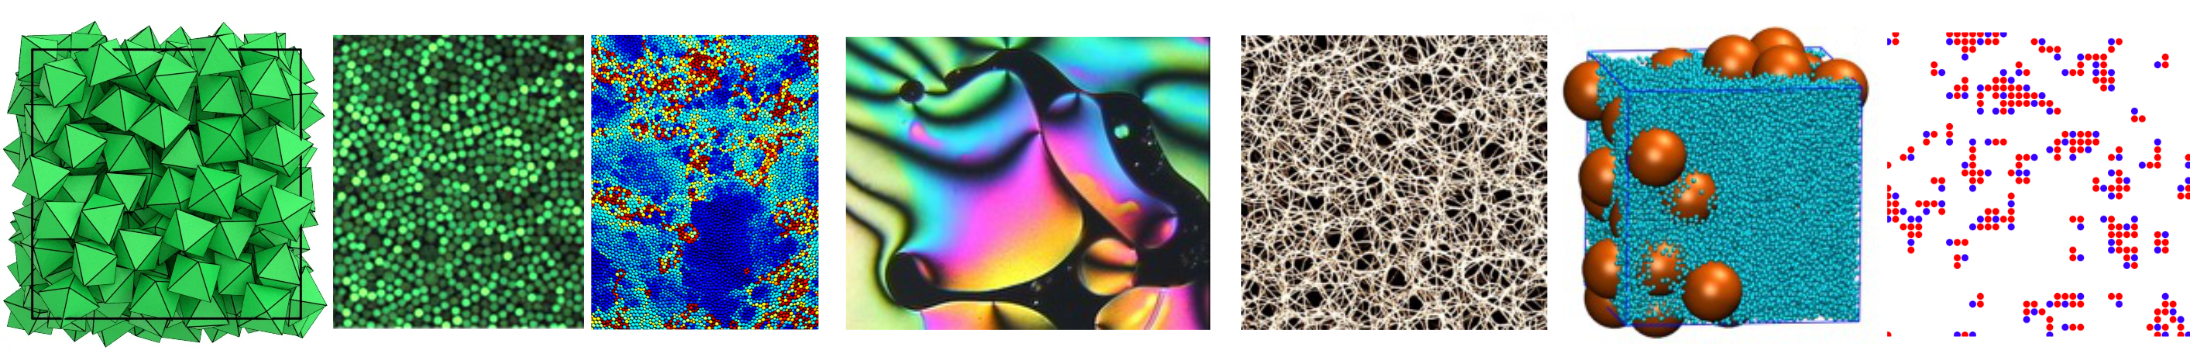
\includegraphics[keepaspectratio]{placeholder_figure_long.png}}\hfill

\section*{Overview}\label{overview}
\addcontentsline{toc}{section}{Overview}

\markright{Overview}

This course introduces your to the theoretical, computational and
experimental aspects of the physics of complex disordered matter.

Complex disordered matter is the study of wide range of systems like
\textbf{polymers}, \textbf{colloids}, \textbf{glasses}, \textbf{gels},
and \textbf{emulsions}, which lack long-range order but exhibit
intricate behaviour. Colloids, suspensions of microscopic particles in a
fluid, are useful for studying disordered structures due to their
observable dynamics. Similarly, polymer systems can form amorphous
solids or glasses when densely packed or cooled, showing solid-like
rigidity despite their disordered structure. These materials often
undergo phase transitions, such as demixing and crystallisation, and
near these transitions, they can display critical phenomena with
extensive fluctuations and correlations.

These various are examples of \textbf{soft matter}. systems In soft
matter systems, the interplay between disorder, softness, and phase
behavior leads to rich physical phenomena, particularly near critical
points where even small changes in external conditions can trigger
large-scale reorganizations and universal behaviour. Glasses, for
instance, exhibit slow relaxation and memory effects, while colloidal
systems may crystallize, phase separate, or become jammed depending on
particle interactions and concentration. Understanding such behaviors
involves studying how microscopic interactions and thermal fluctuations
influence macroscopic properties, especially in non-equilibrium
conditions. Through techniques like scattering, microscopy, rheology,
and simulation, one can explore how disordered soft materials respond to
stress, age, or undergo transitions---insights that are vital for
applications in materials design, biotechnology, and beyond.

This course is organized into three interconnected parts, each offering
a distinct perspective on the study of complex disordered matter.

\begin{itemize}
\tightlist
\item
  \textbf{Part 1: Unifying concepts} (Nigel Wilding) introduces the
  theoretical framework for rationalising complex disordered matter
  which is grounded in statistical mechanics and thermodynamics. We
  emphasize the theory of phase transitions, thermal fluctuations,
  critical phenomena, and stochastic dynamics---providing the essential
  theoretical tools needed to describe and predict the behavior of soft
  and disordered systems.\\
\item
  \textbf{Part 2: Complex disordered matter} (Francesco Turci) explores
  the phenomenology of key examples of complex disordered soft matter
  systems, including colloids, polymers, liquid crystals, glasses, gels,
  and active matter. These systems will be analyzed using the
  theoretical concepts introduced in Part 1, highlighting how disorder,
  interactions, and fluctuations shape their macroscopic behavior.\\
\item
  \textbf{Part 3: Experimental techniques} (Adrian Barnes) focuses on
  the methods of microscopy, and scattering via x-rays, neutrons and
  light that are used to study complex disordered matter, offering
  insight into how their properties are measured and understood in
  real-world contexts.
\end{itemize}

In addition to theory and experiment, computer simulation plays a
central role in soft matter research. This course includes a substantial
coursework component consisting of two computational projects. These
exercises will allow you to apply state-of-the-art simulation techniques
to investigate the complex behavior of disordered systems, bridging
theory and observation through hands-on exploration.

\section*{Delivery and format}\label{delivery-and-format}
\addcontentsline{toc}{section}{Delivery and format}

\markright{Delivery and format}

\begin{itemize}
\item
  Detailed e-notes (accessible via Blackboard) can be viewed on a
  variety of devices. Pdf is also available.
\item
  We will give `traditional' lectures (Tuesdays, Wednesdays, Fridays) in
  which we use slides to summarise and explain the lecture content.
  Questions are welcome (within reason\ldots)
\item
  Try to read ahead in the notes, then come to lectures, listen to the
  explanations and then reread the notes.
\item
  Rewriting the notes or slides to express your own thoughts and
  understanding, or annotating a pdf copy can help wire the material
  into your own way of thinking.
\item
  There are problem classes (Thursdays) where you can try problem sheets
  and seek help. Lecturers may go over some problems with the class.
\item
  The navigation bar on the left will allow you to access the lecture
  notes and problem sets.
\end{itemize}

\section*{Intended learning outcomes}\label{intended-learning-outcomes}
\addcontentsline{toc}{section}{Intended learning outcomes}

\markright{Intended learning outcomes}

The course will

\begin{itemize}
\tightlist
\item
  Introduce you to the qualitative features of a range of complex and
  disordered systems and the experimental techniques used to study them.
\item
  Introduce you to a range of model systems and theoretical techniques
  used to elucidate the physics of complex disordered matter.
\item
  Provide you with elementary computational tools to model complex
  disordered systems numerically and predict their properties.
\item
  Allow you to apply your physics background to understand a variety of
  systems of inter-disciplinary relevance.
\item
  Connect with the most recent advances in the research on complex
  disordered matter.
\end{itemize}

\section*{Contact details}\label{contact-details}
\addcontentsline{toc}{section}{Contact details}

\markright{Contact details}

The course will be taught by

\begin{itemize}
\tightlist
\item
  Prof Nigel B. Wilding (unit director): nigel.wilding@bristol.ac.uk
\item
  Dr Francesco Turci: F.Turci@bristol.ac.uk
\item
  Dr Adrian Barnes: a.c.barnes@bristol.ac.uk
\end{itemize}

\section*{Questions and comments}\label{questions-and-comments}
\addcontentsline{toc}{section}{Questions and comments}

\markright{Questions and comments}

If you have any questions about the course, please don't hesitate to
contact the relevant lecturer, either by email (see above) or in a
problems class.

Finally, this is a new course for 2025/26. If you find any errors or
mistakes or something which isn't clear, please let us know by email, or
fill in this anonymous form:

\begin{tcolorbox}[enhanced jigsaw, breakable, colframe=quarto-callout-note-color-frame, colback=white, arc=.35mm, left=2mm, leftrule=.75mm, bottomrule=.15mm, rightrule=.15mm, toprule=.15mm, opacityback=0]

\href{https://forms.office.com/e/6uL2Bd5QGq}{Submit an
error/mistake/query}

\end{tcolorbox}

\bookmarksetup{startatroot}

\chapter*{Recommended texts and literature}\label{literature}
\addcontentsline{toc}{chapter}{Recommended texts and literature}

\markboth{Recommended texts and literature}{Recommended texts and
literature}

\emph{Needs to be tidied and unified.}

\emph{Experimental textbooks?}

One motivation for supplying you with detailed notes for this course
course is the absence of a wholly ideal text book. However, it should be
stressed that while these notes approach (in places) the detail of a
book, the notes are not fully comprehensive and should be regarded as
the `bare bones' of the course, to be fleshed out via your own reading
and supplementary note taking. To this end perhaps the most appropriate
textbooks are:

A good book at the right level for the phase transitions and critical
phenomena part of the course is

\begin{itemize}
\tightlist
\item
  \textbf{\href{https://bris.on.worldcat.org/search/detail/24699159?queryString=yeomans\%20statistical&clusterResults=true&stickyFacetsChecked=true&groupVariantRecords=false&newsArticles=off&bookReviews=off}{J.M.
  Yeomans: Statistical Mechanics of Phase Transitions}}
\end{itemize}

A good book covering all aspects of this part of the course including
non-equilibrium systems is

\begin{itemize}
\tightlist
\item
  \textbf{\href{https://bris.on.worldcat.org/search/detail/941821555?queryString=chandler\%20statistical&clusterResults=true&stickyFacetsChecked=true&groupVariantRecords=false&newsArticles=off&bookReviews=off}{D.
  Chandler: Introduction to Modern Statistical Mechanics}}
\end{itemize}

You might also wish to dip into the introductory chapters of the
following more advanced texts

\begin{itemize}
\item
  \textbf{\href{https://bris.on.worldcat.org/search/detail/25914535?queryString=Lectures\%20on\%20Phase\%20Transitions\%20and\%20the\%20Renormalization\%20Group&clusterResults=true&stickyFacetsChecked=true&groupVariantRecords=false&newsArticles=off&bookReviews=off}{N
  Goldenfeld: Lectures on Phase Transitions and the Renormalization
  Group}}
\item
  \textbf{\href{https://bris.on.worldcat.org/search/detail/861559276?queryString=\%20The\%20Theory\%20of\%20Critical\%20Phenomena&clusterResults=true&stickyFacetsChecked=true&groupVariantRecords=false&newsArticles=off&bookReviews=off}{J.J.
  Binney, N.J. Dowrick, A.J.Fisher and M.E.J. Newman: The Theory of
  Critical Phenomena}}
\end{itemize}

For revision on thermodynamics and statistical mechanics

\begin{itemize}
\tightlist
\item
  \textbf{\href{https://bris.on.worldcat.org/search/detail/15487191?queryString=F.\%20Mandl&clusterResults=true&stickyFacetsChecked=true&groupVariantRecords=false}{F.
  Mandl: Statistical Physics}}.
\end{itemize}

For Stochastic dynamics

\begin{itemize}
\tightlist
\item
  \textbf{\href{https://bris.on.worldcat.org/search/detail/162131511?queryString=Stochastic\%20Processes\%20in\%20Physics\%20and\%20Chemistry\%20by\%20N.G.\%20van\%20Kampen&clusterResults=true&stickyFacetsChecked=true&groupVariantRecords=false}{N.G.
  van Kampen: Stochastic processess in Physics and Chemistry}}
\end{itemize}

The best overall text for part 2 of the course is: R.A.L Jones, Soft
Condensed Matter, Oxford University Press.

Additionally, the following more specialised texts should also be
useful. They can be found in the University Library under the stated
shelfmark.

\subsection*{Colloids}\label{colloids}
\addcontentsline{toc}{subsection}{Colloids}

\begin{enumerate}
\def\labelenumi{(\arabic{enumi})}
\tightlist
\item
  D.F.Evans, H.Wennerström: The Colloidal Domain - Where Physics,
  Chemistry, Biology, and Technology Meet. VCH Publishers (1994).
\item
  R.J.Hunter: Introduction to Modern Colloid Science. Oxford University
  Press (1993).
\item
  W.B.Russel, D.A.Saville, W.R.Schowalter: Colloidal Dispersions
  Cambridge University Press (1989).
\item
  D.H.Everett: Basic Principles of Colloid Science.
\end{enumerate}

Royal Society of Chemistry Paperbacks (1988)

\subsection*{Polymers and surfactants}\label{polymers-and-surfactants}
\addcontentsline{toc}{subsection}{Polymers and surfactants}

\begin{enumerate}
\def\labelenumi{(\arabic{enumi})}
\tightlist
\item
  R.J. Young and P.A. Lovell: Introduction to polymers .
\item
  M. Doi: Introduction to polymer physics
\item
  J.Israelachvili, Intermolecular and Surface Forces, Academic Press
  (1992), Chs. 16 and 17
\end{enumerate}

\subsection*{Glasses}\label{glasses}
\addcontentsline{toc}{subsection}{Glasses}

\begin{enumerate}
\def\labelenumi{(\arabic{enumi})}
\tightlist
\item
  J. Zarzycki; Glasses and the vitreous state. Cambridge University
  Press (1991).
\end{enumerate}

\part{Unifying concepts}

\chapter{Introduction to phase behaviour and enhanced
fluctuations}\label{introduction-to-phase-behaviour-and-enhanced-fluctuations}

A phase transition can be defined as a macroscopic rearrangment of the
internal constituents of a system in response to a change in the
thermodynamic conditions to which they are subject. A wide variety of
physical systems undergo such transitions. Understanding the properties
of phase transitions is fundamental to the study of soft and complex
matter, as these systems often exhibit rich and subtle transformations
between different states of organization. Whether in colloidal
suspensions, polymer blends, liquid crystals, or biological materials,
phase transitions underpin a wide range of physical behaviours, from
self-assembly and pattern formation to critical phenomena and dynamical
arrest. By analysing how macroscopic phases emerge from microscopic
interactions and external conditions, one gains crucial insight into the
principles that govern structure, stability, and functionality in these
intricate systems. As such, an understanding of phase transitions not
only enriches theoretical understanding but also informs practical
applications across materials science, biophysics, and nanotechnology.
For these reasons we will devote a large proportion of this course to
the study of phase transitions.

Two classic examples of systems displaying phase transitions are the
ferromagnet and fluid systems. For the magnet, a key observable is the
magnetisation defined as the magnetic moment per spin, given by
\(m=M/N\), with \(N\) the number of spins. \(m\) can be positive or
negative, dependent on whether the spins are aligned `up' or `down'. As
the temperature of a ferromagnet is increased, its net magnetisation
\(|m|\) is observed to decrease smoothly, until at a certain temperature
known as the critical temperature, \(T_c\), it vanishes altogether (see
left part of Figure~\ref{fig-isingpd}). We define the magnetisation to
be the \emph{order parameter} of this phase transition.

One can also envisage applying a magnetic field \(H\) to the system
which, depending on its sign (i.e.~whether it is aligned (positive) or
anti-aligned (negative) relative to the magnetisation axis), favours up
or down spin states respectively, as shown schematically in
Figure~\ref{fig-isingpd} (right part). Changing the sign of the magnetic
field \(H\) for \(T<T_c\) leads to a phase transition chacterised by a
discontinuous jump in \(m\). We shall explore this behaviour in more
detail in section 6.

\begin{figure}

\centering{

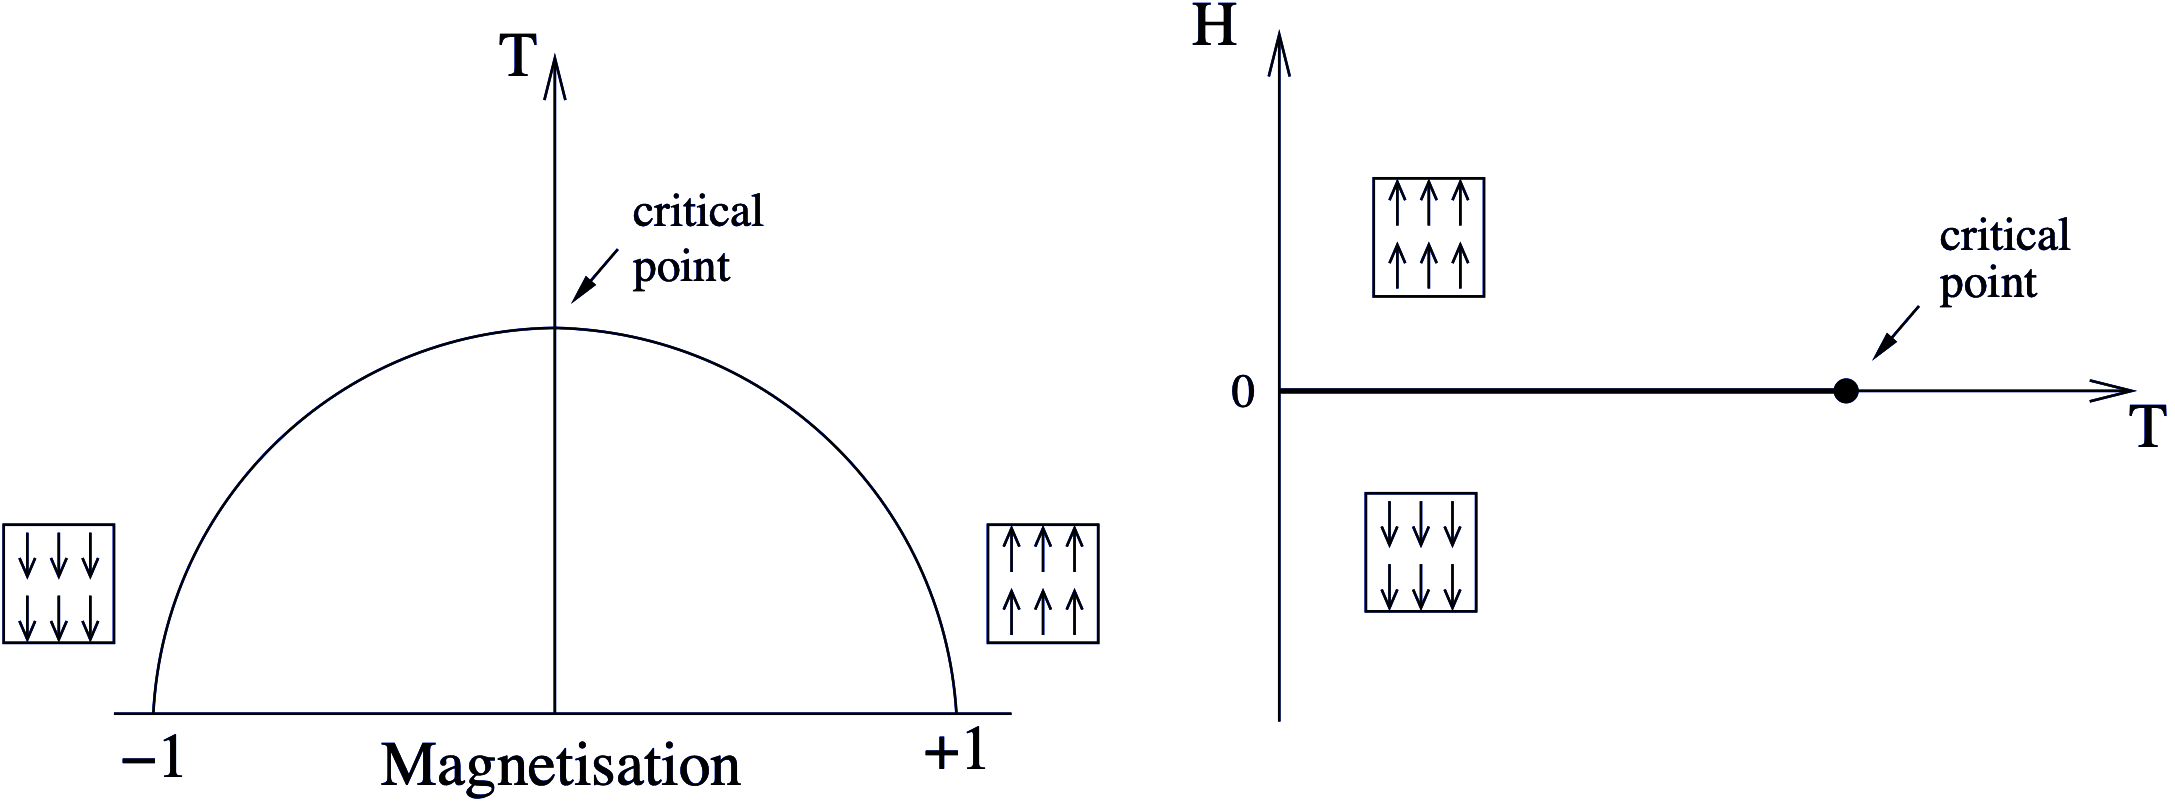
\includegraphics[width=0.8\linewidth,height=\textheight,keepaspectratio]{phase-transitions/Figs/isingpd_color.png}

}

\caption{\label{fig-isingpd}Phase diagram of a simple magnet
(schematic). Left: magnetisation as a function of temperature for zero
applied magnetic field, \(H=0\). Right: Applying a magnetic field that
is aligned or antialigned with the direction of the magnetisation leads
to a phase transition. The \(H=0\) axis at \(T<T_c\) is the coexistence
curve for which positive and negative magnetisations are equally
likely.}

\end{figure}%

Similarly, a change of state from liquid to gas can be induced in a
fluid system (though not in an ideal gas) simply by raising the
temperature. Typically the liquid-vapour transition is abrupt,
reflecting the large number density difference between the states either
side of the transition. However the abruptness of this transition can be
reduced by applying pressure. At one particular pressure and temperature
the discontinuity in the density difference between the two states
vanishes and the two phases coalesce. These conditions of pressure and
temperature serve to locate the critical point for the fluid. We define
the density difference \(\rho_{liq}-\rho_{vap}\) to be the order
parameter for the liquid-gas phase transition. We shall meet order
parameters for other, more complex, systems in
Section~\ref{sec-landau-theory},

\begin{figure}

\centering{

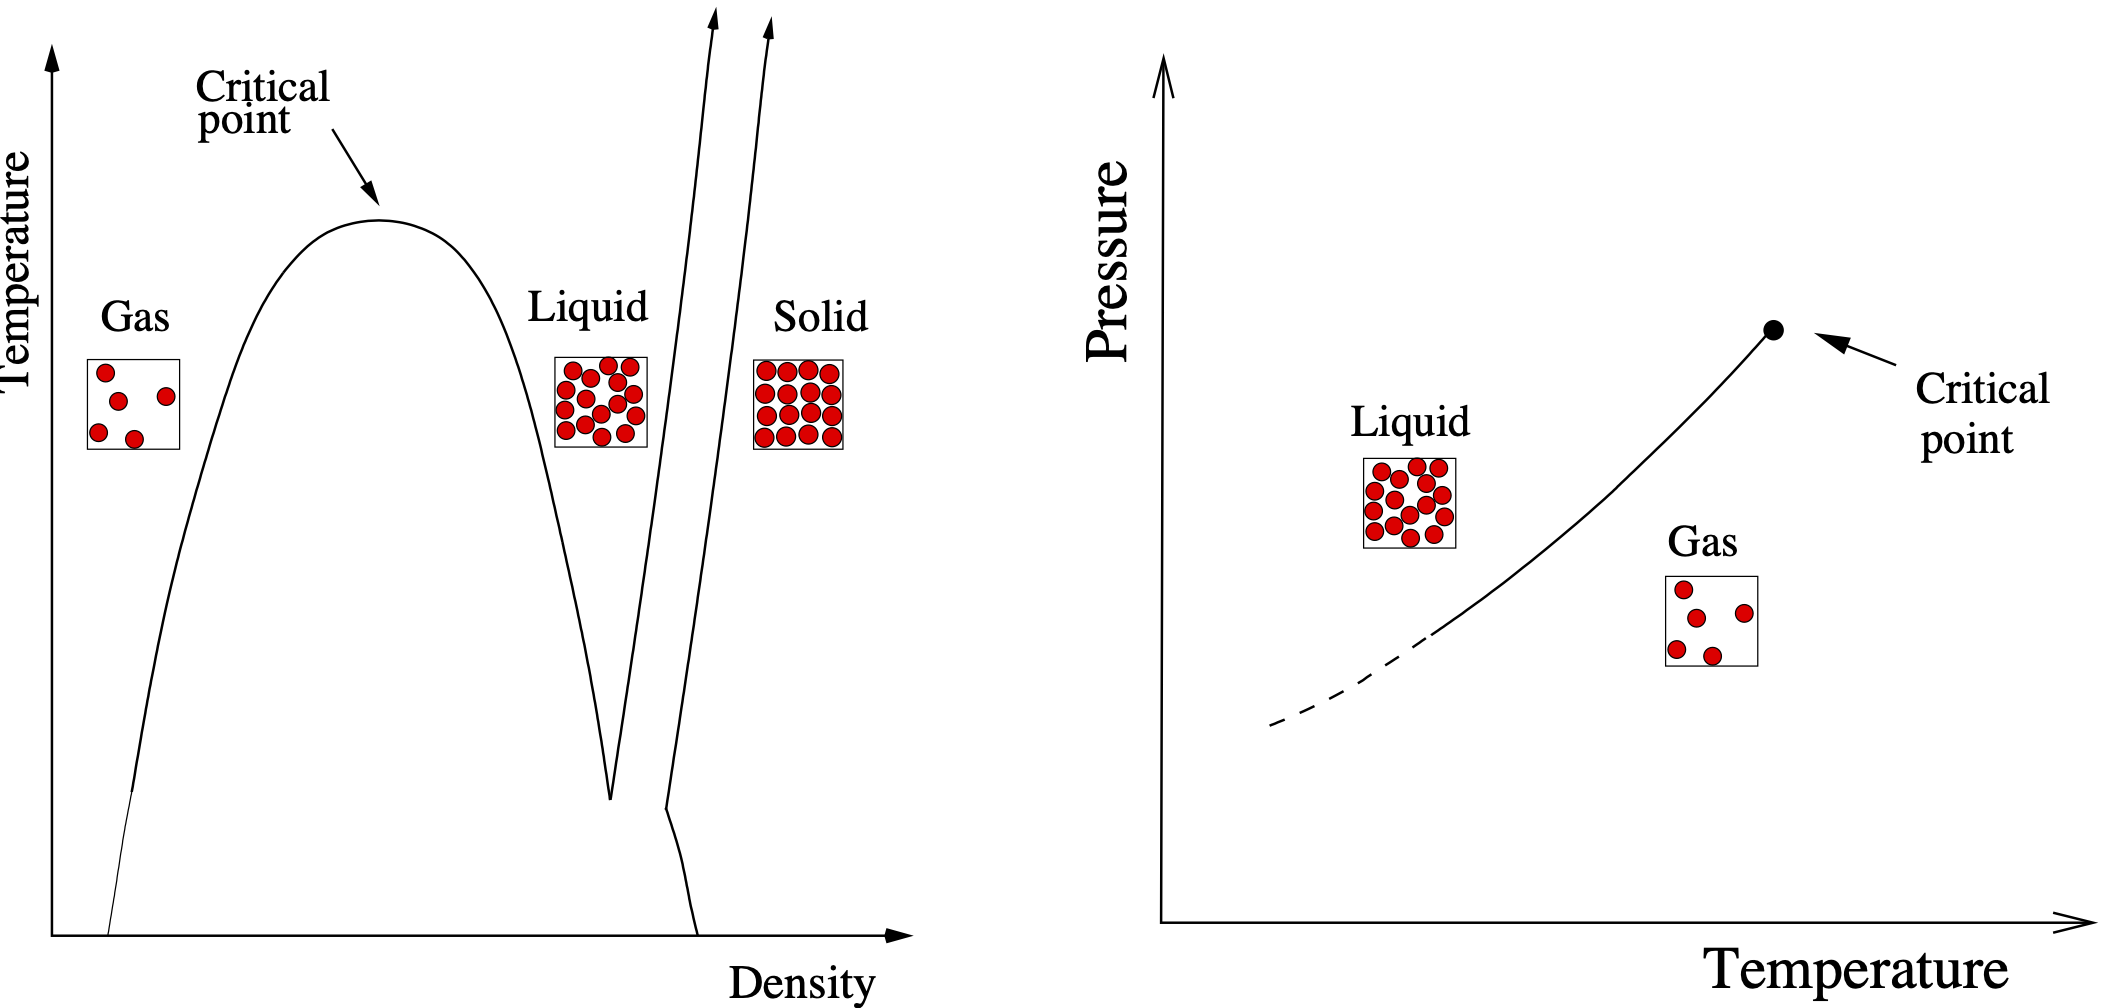
\includegraphics[width=0.8\linewidth,height=\textheight,keepaspectratio]{phase-transitions/Figs/ljpd1.png}

}

\caption{\label{fig-fluidpd}Phase diagram of a simple fluid (schematic)}

\end{figure}%

In the vicinity of a critical point, a system displays a host of
remarkable behaviors known as \emph{critical phenomena}. Chief among
these is the divergence of thermal response functions---such as specific
heat, compressibility, or magnetic susceptibility---which signal an
enhanced sensitivity to external perturbations. These singularities
arise from the emergence of large-scale cooperative interactions among
the system's microscopic constituents, as measured by a diverging
\emph{correlation length} (see Chapter~\ref{sec-background}). One
visually striking manifestation of this is \emph{critical opalescence},
particularly observed in fluids like CO\(_2\). As carbon dioxide nears
its critical temperature and pressure, the distinction between its
liquid and gas phases vanishes, giving rise to huge fluctuations in
density. These fluctuations scatter visible light, rendering the fluid
milky or opalescent. This scattering effect directly reflects the
long-range correlations developing within the fluid. The movie below
illustrates the effect as the critical temperature of CO\(_2\) is
approached from above. Note the appearence of a liquid-vapour interface
(meniscus) as the system enters the two-phase region.

\url{Movies/critical_point_1.mp4}

The recalcitrant problem posed by the critical region is how best to
incorporate such collective effects within the framework of a rigorous
mathematical theory that affords both physical insight and quantitative
explanation of the observed phenomena. This matter has been (and still
is!) the subject of intense theoretical activity.

The importance of the critical point stems largely from the fact that
many of the phenomena observed in its vicinity are believed to be common
to a whole range of apparently quite disparate physical systems. Systems
such as liquid mixtures, superconductors, liquid crystals, ferromagnets,
antiferromagnets and molecular crystals may display identical behaviour
near criticality. This observation implies a profound underlying
similarity among physical systems at criticality, regardless of many
aspects of their distinctive microscopic nature. These ideas have found
formal expression in the so-called `universality hypothesis' which,
since its inception in the 1970s, has enjoyed considerable success.

In the next few lectures, principal aspects of the contemporary
theoretical viewpoint of phase transitions and critical phenomena will
be reviewed. Mean field theories of phase transitions will be discussed
and their inadequacies in the critical region will be exposed. The
phenomenology of the critical region will we described including power
laws, critical exponents and their relationship to scaling phenomena.
These will be set within the context of the powerful renormalisation
group technique. The notion of universality as a phenomenological
hypothesis will be introduced and its implications for real and model
systems will be explored. Finally, the utility of finite-size scaling
methods for computer studies of critical phenomena will be discussed,
culminating in the introduction of a specific technique suitable for
exposing universality in model systems. Thereafter we will consider some
foundational concepts in the dynamics of complex disorderd matters. We
shall look at the processes by which one phase transform into another
and introduce differential equations that allow us to deal with the
inherent stochasticity of thermal systems. The wider applicability of
these unifying concepts to complex disordered systems such as colloids,
polymers, liquid crystals and glasses will be covered in part 2 of the
course.

\chapter{Key concepts for phase transitions}\label{sec-background}

\section{Observables and expectation
values}\label{observables-and-expectation-values}

In seeking to describe phase transition and critical phenomena, it is
useful to have a quantitative measure of the difference between the
phases: this is the role of the \emph{order parameter}, \(Q\). In the
case of the fluid, the order parameter is taken as the difference
between the densities of the liquid and vapour phases. In the
ferromagnet it is taken as the magnetisation. As its name suggest, the
order parameter serves as a measure of the kind of orderliness that sets
in when the temperature is cooled below a critical temperature.

Our first task is to give some feeling for the principles which underlie
the ordering process. Referring back to \textbf{?@sec-canonical}, the
probability \(p_a\) that a physical system at temperature \(T\) will
have a particular microscopic arrangement (alternatively referred to as
a `configuration' or `state'), labelled \(a\), of energy \(E_a\) is

\begin{equation}\phantomsection\label{eq-probs}{
p_a=\frac{1}{Z}e^{-E_a/k_BT}
}\end{equation}

The prefactor \(Z^{-1}\) is the \emph{partition function}: since the
system must always have \emph{some} specific arrangement, the sum of the
probabilities \(p_a\) must be unity, implying that

\begin{equation}\phantomsection\label{eq-partition}{
Z=\sum_ae^{-E_a/k_BT}
}\end{equation} where the sum extends over all possible microscopic
arrangements.

These equations assume that physical system evolves rapidly (on the
timescale of typical observations) amongst all its allowed arrangements,
sampling them with the probabilities~Equation~\ref{eq-probs} the
expectation value of any physical observable \(O\) will thus be given by
averaging \(O\) over all the arrangements \(a\), weighting each
contribution by the appropriate probability:

\begin{equation}\phantomsection\label{eq-observable}{\overline {O}=\frac{1}{Z}\sum_a O_a e^{-E_a/k_BT}
}\end{equation}

Sums like Equation~\ref{eq-observable} are not easily evaluated.
Nevertheless, some important insights follow painlessly. Consider the
case where the observable of interest is the order parameter, or more
specifically the magnetisation of a ferromagnet.

\begin{equation}\phantomsection\label{eq-op}{
Q=\frac{1}{Z}\sum_a Q_a e^{-E_a/k_BT}
}\end{equation}

It is clear from Equation~\ref{eq-probs} that at very low temperature
the system will be overwhelmingly likely to be found in its minimum
energy arrangements (ground states). For the ferromagnet, these are the
fully ordered spin arrangements having magnetisation \(+1\), or \(-1\).

Now consider the high temperature limit. The enhanced weight that the
fully ordered arrangement carries in the sum of Equation~\ref{eq-op} by
virtue of its low energy, is now no longer sufficient to offset the fact
that arrangements in which \(Q_a\) has some intermediate value, though
each carry a smaller weight, are vastly greater in number. A little
thought shows that the arrangements which have essentially zero
magnetisation (equal populations of up and down spins) are by far the
most numerous. At high temperature, these disordered arrangements
dominate the sum in Equation~\ref{eq-op} and the order parameter is
zero.

The competition between energy-of-arrangements weighting (or simply
`energy') and the `number of arrangements' weighting (or `entropy') is
then the key principle at work here. The distinctive feature of a system
with a critical point is that, in the course of this competition, the
system is forced to choose amongst a number of macroscopically different
sets of microscopic arrangements.

Finally in this section, we note that the probabilistic (statistical
mechanics) approach to thermal systems outlined above is completely
compatible with classical thermodynamics. Specifically, the bridge
between the two disciplines is provided by the following equation

\begin{equation}\phantomsection\label{eq-free}{
F=-k_BT \ln Z
}\end{equation}

where \(F\) is the ``Helmholtz free energy''. All thermodynamic
observables, for example the order parameter \(Q\), and response
functions such as the specific heat or magnetic susceptibility are
obtainable as appropriate derivatives of the free energy. For instance,
utilizing Equation~\ref{eq-partition}, one can readily verify (try it as
an exercise!) that the average internal energy is given by

\[\overline{E}=-\frac{\partial \ln Z}{\partial \beta},\]

where \(\beta=(k_BT)^{-1}\).

The relationship between other thermodynamic quantities and derivatives
of the free energy are given in fig. Figure~\ref{fig-thermo}

\begin{figure}

\centering{

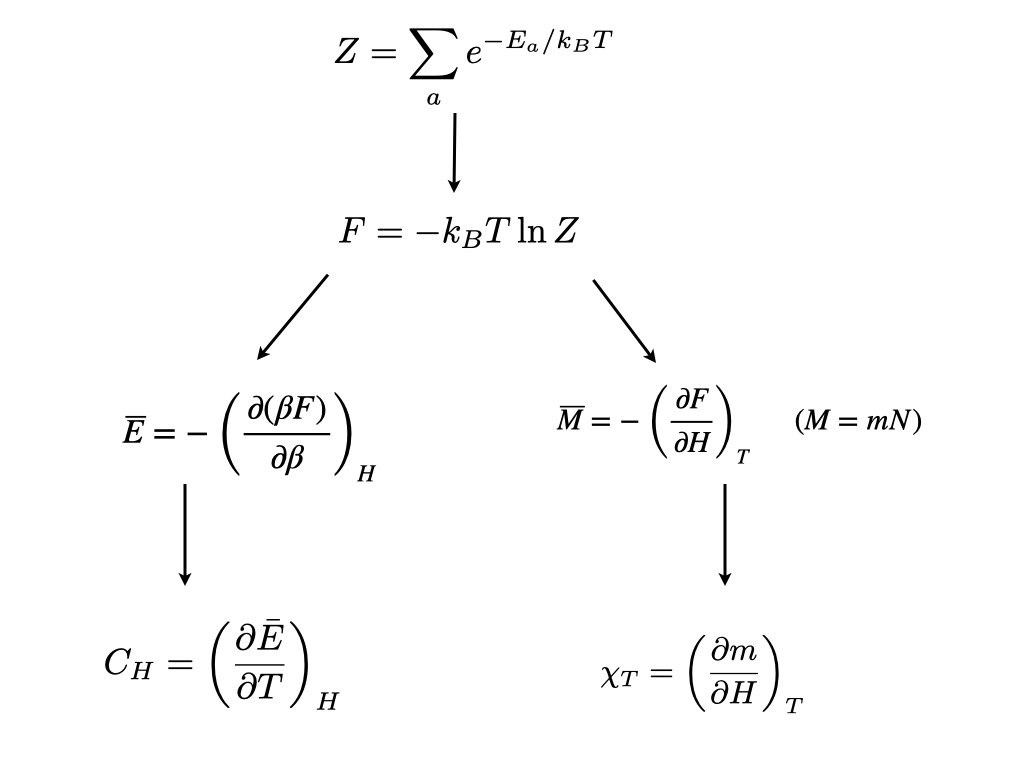
\includegraphics[width=0.8\linewidth,height=\textheight,keepaspectratio]{phase-transitions/Figs/thermo.png}

}

\caption{\label{fig-thermo}Relationships between the partition function
and thermodynamic observables}

\end{figure}%

\section{Correlations}\label{sec-correlations}

\subsection{Spatial correlations}\label{spatial-correlations}

The two-point connected correlation function measures how fluctuations
at two spatial points are statistically related. For a scalar field
\(\phi(\vec{R})\), which could represent eg. the local magnetisation
\(m\) in a magnet at position vector \(\vec{R}\), or the local particle
number density \(\rho\) in a fluid, it is defined as:

\[
C(r) = \langle \phi(\vec{R}) \phi(\vec{R} + \vec{r}) \rangle - \langle \phi(\vec{R}) \rangle^2,
\]

where \(\langle \cdot \rangle\) denotes an ensemble or spatial average
over all \(\vec{R}\), and \(r = |\vec{r}|\) is the spatial separation
between the two points.

\(C(r)\) quantifies the spatial extent over which field values are
correlated and in homogeneous and isotropic systems, it depends only on
the separation \(r\).

If \(C(r)\) decays quickly, we say that correlations are short-ranged.
Typically this occurs well away from criticality and takes the form of
exponential decay

\[
  C(r) \sim e^{-r/\xi}
  \] where the correlation length \(\xi\) is the characteristic scale
over which correlations decay.

Near a critical point \(C(r)\) decays more slowly - in a power-law
fashion - and correlations are long-ranged.

\[
  C(r) \sim r^{-(d - 2 + \eta)}
  \] where \(d\) is the spatial dimension and \(\eta\) is a critical
exponent.

In isotropic fluids and particle systems, a closely related and more
directly measurable quantity (particularly in simulations) is the
\textbf{radial distribution function} \(g(r)\), which describes how
particle density varies as a function of distance from a reference
particle. For such systems, the two-point correlation function of the
number density field \(\rho(\vec{r})\) is related to \(g(r)\) as
follows:

\[
g(r) = 1+\frac{C(r)}{\rho^2},
\] where \(\rho\) is the average number density. This relation shows
that \(g(r)\) encodes the same spatial correlations as \(C(r)\), but in
a form that is more natural for discrete particle systems. Note that by
definition \(g(r)\to 1\) in the absence of correlations ie. when
\(C(r)=0\). This is typically the case for \(r\gg\xi\).

Experimentally one doesn't typically have direct access to \(C(r)\), but
rather its Fourier transform known as the \textbf{structure factor}

\[
S(k) = \int d^d r \, e^{-i \vec{k} \cdot \vec{r}} \, C(r),
\] where \(k\) is the scattering wavevector.

In equilibrium:

\begin{itemize}
\item
  For short-range correlations (finite \(\xi\)), \(S(k)\) typically has
  a Lorentzian form: \[
  S(k) \sim \frac{1}{k^2 + \xi^{-2}}.
  \]
\item
  At criticality (where \(\xi \to \infty\)), \(S(k)\) follows a power
  law: \[
  S(k) \sim k^{-2 + \eta}.
  \]
\end{itemize}

This relation enables the extraction of \(\xi\) from experimental or
simulation data, especially via scattering techniques.

\subsection{Temporal correlations}\label{temporal-correlations}

Consider a thermodynamic variable \(x\) with zero mean that fluctuates
over time. Examples include the local magnetization in a magnetic system
or the local density in a fluid. Here, \(x\) represents a deviation from
the average value --- a fluctuation.

We're interested in how such fluctuations are correlated over time when
the system is in thermal equilibrium. For instance, if \(x\) is positive
at some time \(t\), it's more likely to remain positive shortly after.

These temporal correlations are characterized by the two-time
correlation function (also known as an auto-correlation function):

\[
\langle x(\tau) x(\tau + t) \rangle
\]

In equilibrium, the correlation function must be independent of the
starting time \(\tau\). Therefore, we define:

\[
\langle x(\tau) x(\tau + t) \rangle = M_{xx}(t)
\]

That is, \(M_{xx}(t)\) depends only on the time difference \(t\).

We typically expect \(M_{xx}(t)\) to decay exponentially over a
characteristic correlation time \(t_c\):

\[
M_{xx}(t) \sim \exp(-t / t_c)
\]

\begin{figure}

\centering{

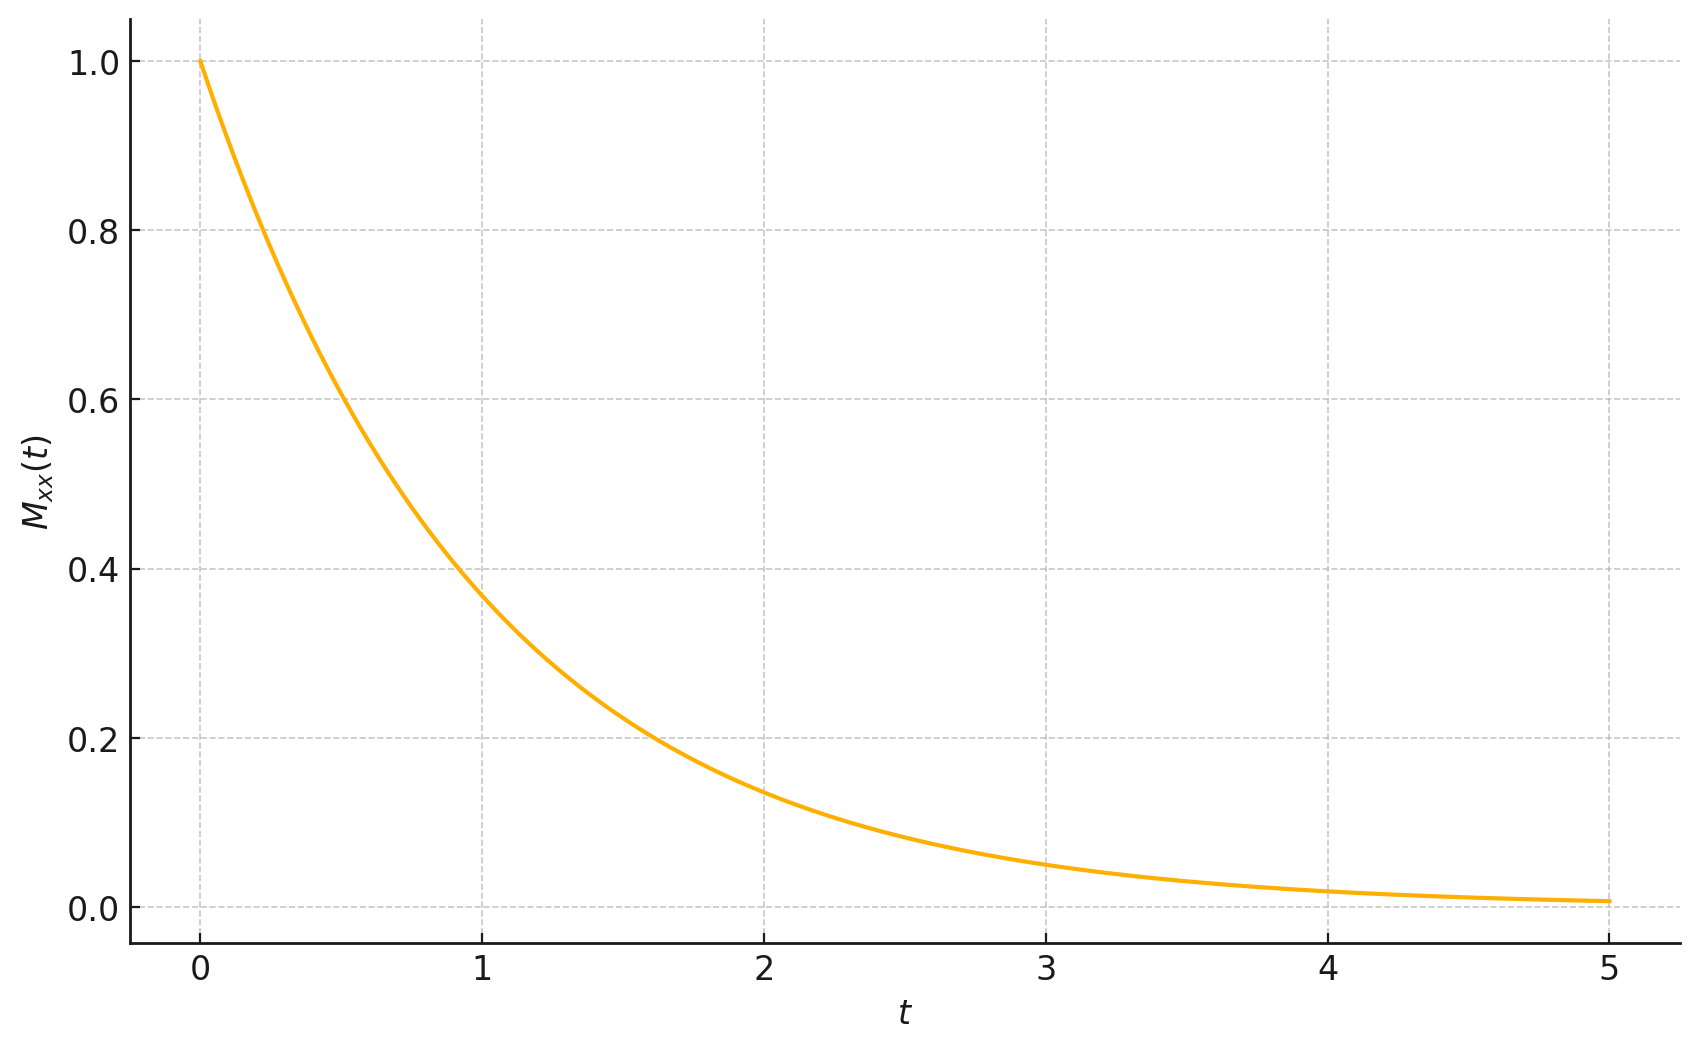
\includegraphics[width=0.6\linewidth,height=\textheight,keepaspectratio]{phase-transitions/Figs/Mxx(t).png}

}

\caption{\label{fig-Mxx}Sketch of \(M_{xx}(t)\) against \(t\)}

\end{figure}%

This exponential decay reflects how the memory of fluctuations fades
with time.

Now consider two different fluctuating variables, \(x\) and \(y\) (e.g.,
local magnetizations at different positions). Their cross-correlation
function is defined as:

\[
\langle x(\tau) y(\tau + t) \rangle = M_{xy}(t)
\]

This defines the elements of a dynamic correlation matrix, of which
\(M_{xx}(t)\) is the diagonal.

\chapter{The approach to criticality}\label{sec:approach}

It is a matter of experimental fact that the approach to criticality in
a given system is characterized by the divergence of various
thermodynamic observables. Let us remain with the archetypal example of
a critical system, the ferromagnet, whose critical temperature will be
denoted as \(T_c\). For temperatures close to \(T_c\), the magnetic
response functions (the magnetic susceptibility \(\chi\) and the
specific heat) are found to be singular functions, diverging as a
\emph{power} of the reduced (dimensionless) temperature \(t \equiv
(T-T_c)/T_c\):-

\begin{equation}\phantomsection\label{eq-chipow}{
\chi \equiv \frac{\partial M}{\partial H}\propto t^{-\gamma} ~~~~ (H=0) 
}\end{equation}

(where \(M=mN\)), \begin{equation}\phantomsection\label{eq-Cv}{
C_H \equiv \frac{\partial E}{\partial T}\propto t^{-\alpha} ~~~~ (H=\textrm{ constant}) 
}\end{equation}

Another key quantity is the correlation length \(\xi\), which measures
the distance over which fluctuations of the magnetic moments are
correlated. This is observed to diverge near the critical point with an
exponent \(\nu\).

\begin{equation}\phantomsection\label{eq-corr}{
\xi \propto t^{-\nu} ~~~~ (T > T_c,\: H=0)
}\end{equation}

Similar power law behaviour is found for the order parameter \(Q\) (in
this case the magnetisation) which vanishes in a singular fashion (it
has infinite gradient) as the critical point is is approached as a
function of temperature:

\begin{equation}\phantomsection\label{eq-mag}{
m \propto t^{\beta} ~~~~ (T < T_c,\: H=0) 
}\end{equation} (here the symbol \(\beta\), is not to be confused with
\(\beta=1/k_BT\)-- this unfortunately is the standard notation.)

Finally, as a function of magnetic field:

\begin{equation}\phantomsection\label{eq-field}{m \propto h^{1/\delta} ~~~~ (T = T_c,\: H>0) .}\end{equation}
with \(h=(H-H_c)/H_c\), the reduced magnetic field.

As examples, the behaviour of the magnetisation and correlation length
are plotted in Figure~\ref{fig-sing} as a function of \(t\).

\begin{figure}

\centering{

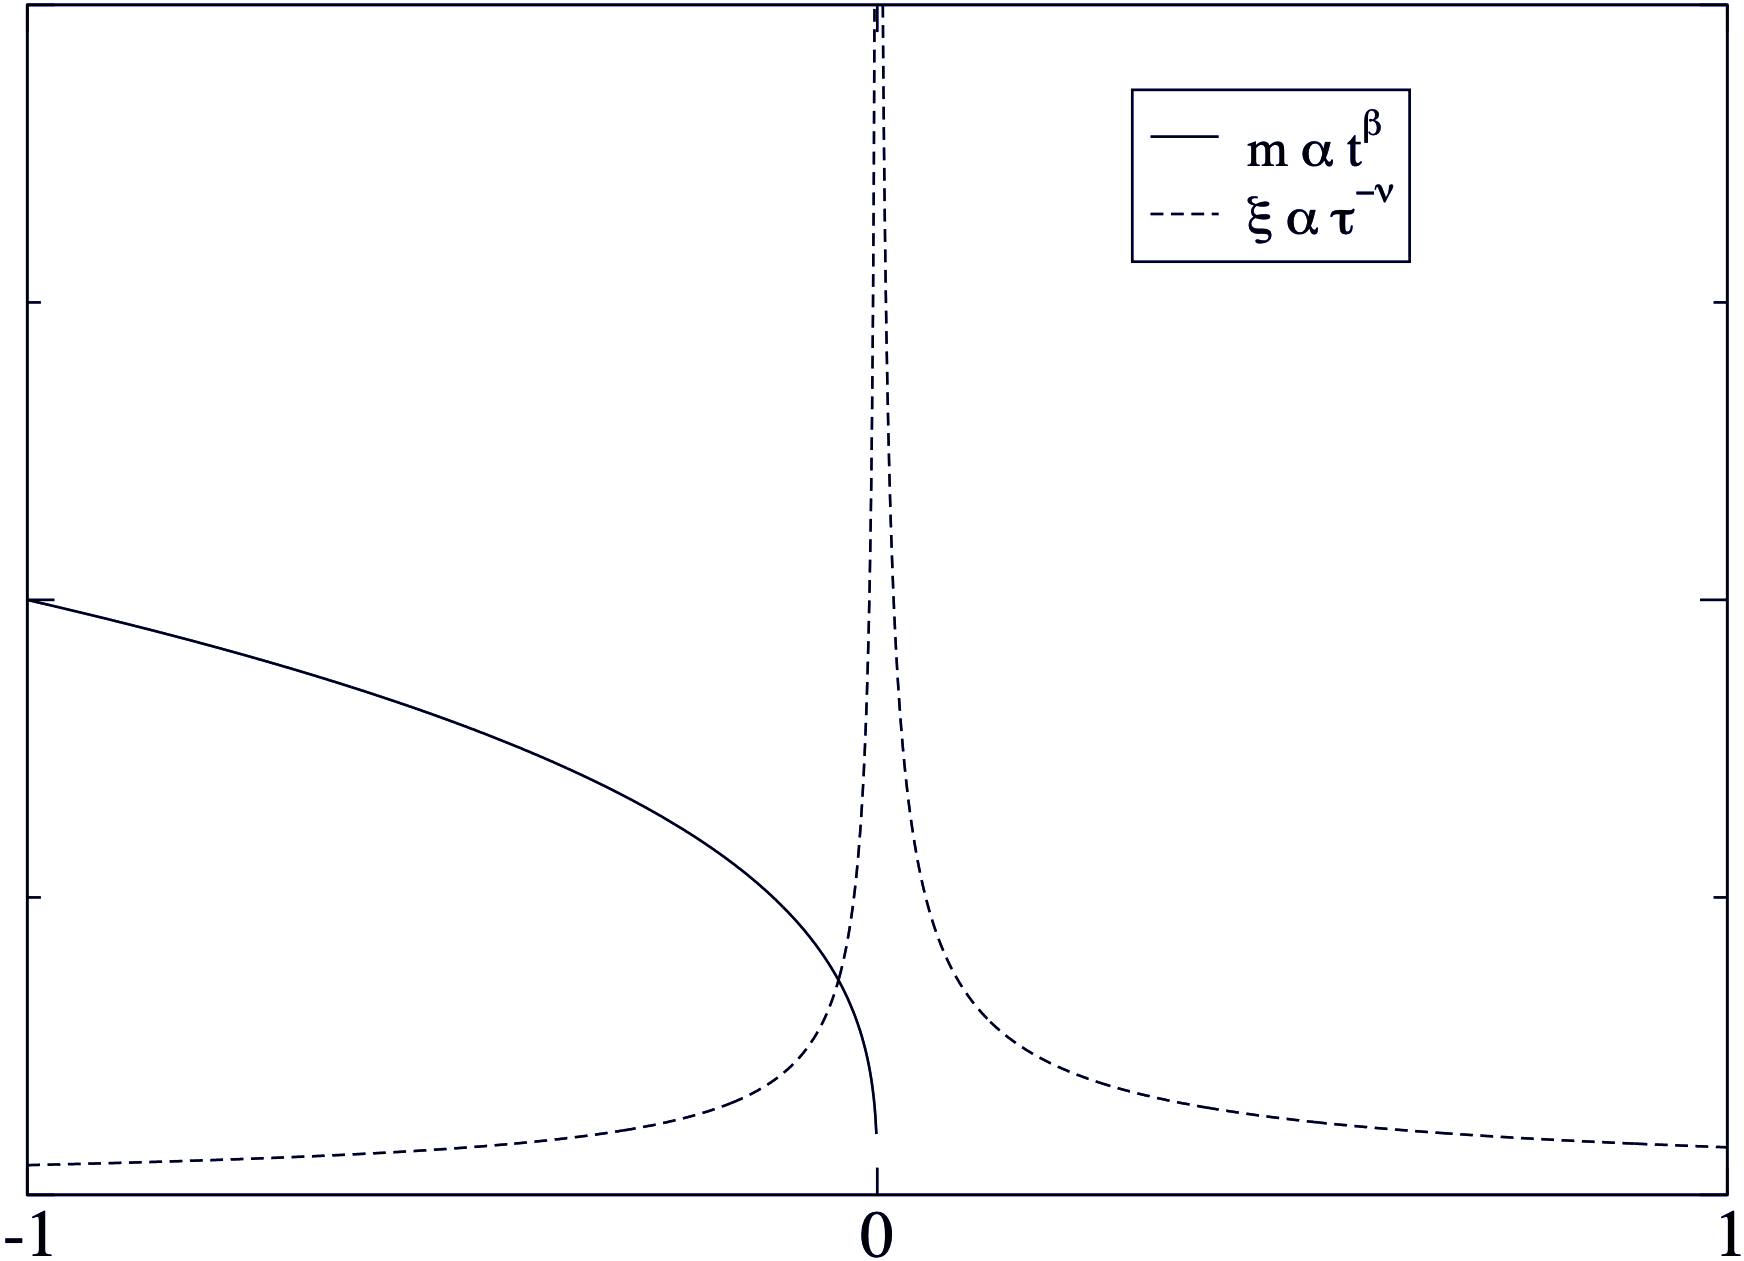
\includegraphics[width=0.5\linewidth,height=\textheight,keepaspectratio]{phase-transitions/Figs/sing_color.png}

}

\caption{\label{fig-sing}Singular behaviour of the correlation length
and order parameter in the vicinity of the critical point as a function
of the reduced temperature \(t\).}

\end{figure}%

The quantities \(\gamma, \alpha, \nu, \beta\) in the above equations are
known as critical exponents. They serve to control the rate at which the
various thermodynamic quantities change on the approach to criticality.

Remarkably, the form of singular behaviour observed at criticality for
the example ferromagnet also occurs in qualitatively quite different
systems such as the fluid. All that is required to obtain the
corresponding power law relationships for the fluid is to substitute the
analogous thermodynamic quantities in to the above equations.
Accordingly the magnetisation order parameter is replaced by the density
difference \(\rho_{liq}-\rho_{gas}\) while the susceptibility is
replaced by the isothermal compressibility and the specific heat
capacity at constant field is replaced by the specific heat capacity at
constant volume. The approach to criticality in a variety of
qualitatively quite different systems can therefore be expressed in
terms of a set of critical exponents describing the power law behaviour
for that system (see the book by Yeomans for examples).

Even more remarkable is the experimental observation that the values of
the critical exponents for a whole range of fluids and magnets (and
indeed many other systems with critical points) are \emph{identical}.
This is the phenomenon of \emph{universality}. It implies a deep
underlying physical similarity between ostensibly disparate critical
systems. The principal aim of theories of critical point phenomena is to
provide a sound theoretical basis for the existence of power law
behaviour, the factors governing the observed values of critical
exponents and the universality phenomenon. Ultimately this basis is
provided by the Renormalisation Group (RG) theory, for which K.G. Wilson
was awarded the Nobel Prize in Physics in 1982.

More about the scientists mentioned in this chapter:

\href{https://en.wikipedia.org/wiki/Kenneth_G._Wilson}{Kenneth Wilson}

\chapter{The Ising model: the prototype model for a phase
transition}\label{sec:models}

In order to probe the properties of the critical region, it is common to
appeal to simplified model systems whose behaviour parallels that of
real materials. The sophistication of any particular model depends on
the properties of the system it is supposed to represent. The simplest
model to exhibit critical phenomena is the two-dimensional Ising model
of a ferromagnet. Actual physical realizations of 2-d magnetic systems
do exist in the form of layered ferromagnets such as K\(_2\)CoF\(_4\),
so the 2-d Ising model is of more than just technical relevance.

\section{The 2D Ising model}\label{the-2d-ising-model}

The 2-d spin-\(\frac{1}{2}\) Ising model envisages a regular arrangement
of magnetic moments or `spins' on an infinite plane. Each spin can take
two values, \(+1\) (`up' spins) or \(-1\) (`down' spins) and is assumed
to interact with its nearest neighbours according to the Hamiltonian

\begin{equation}\phantomsection\label{eq-ising}{
{\cal H}_I=-J\sum_{<ij>}s_is_j - H\sum_i s_i
}\end{equation}

where \(J>0\) measures the strength of the coupling between spins and
the sum extends over nearest neighbour spins \(s_i\) and \(s_j\), i.e it
is a sum of the bonds of the lattice. \(H\) is a magnetic field term
which can be positive or negative (although for the time being we will
set it equal to zero). The order parameter is simply the average
magnetisation:

\[m=\frac{1}{N} \langle \sum_i s_i \rangle\:,\] where
\(\langle\cdot\rangle\) means an average over typical configurations
corresponding to the prescribed value of \(J/k_BT\).

The fact that the Ising model displays a phase transition was argued in
Chapter~\ref{sec-background}. Thus at low temperatures for which there
is little thermal disorder, there is a preponderance of aligned spins
and hence a net spontaneous magnetic moment (ie. the system is
ferromagnetic). As the temperature is raised, thermal disorder increases
until at a certain temperature \(T_c\), entropy drives the system
through a continuous phase transition to a disordered spin arrangement
with zero net magnetisation (ie. the system is paramagnetic). These
trends are visible in configurational snapshots from computer
simulations of the 2D Ising model (see Figure~\ref{fig-snapshots}).
Although each spin interacts only with its nearest neighbours, the phase
transition occurs due to cooperative effects among a large number of
spins.

\begin{figure}

\begin{minipage}{0.33\linewidth}

\centering{

\pandocbounded{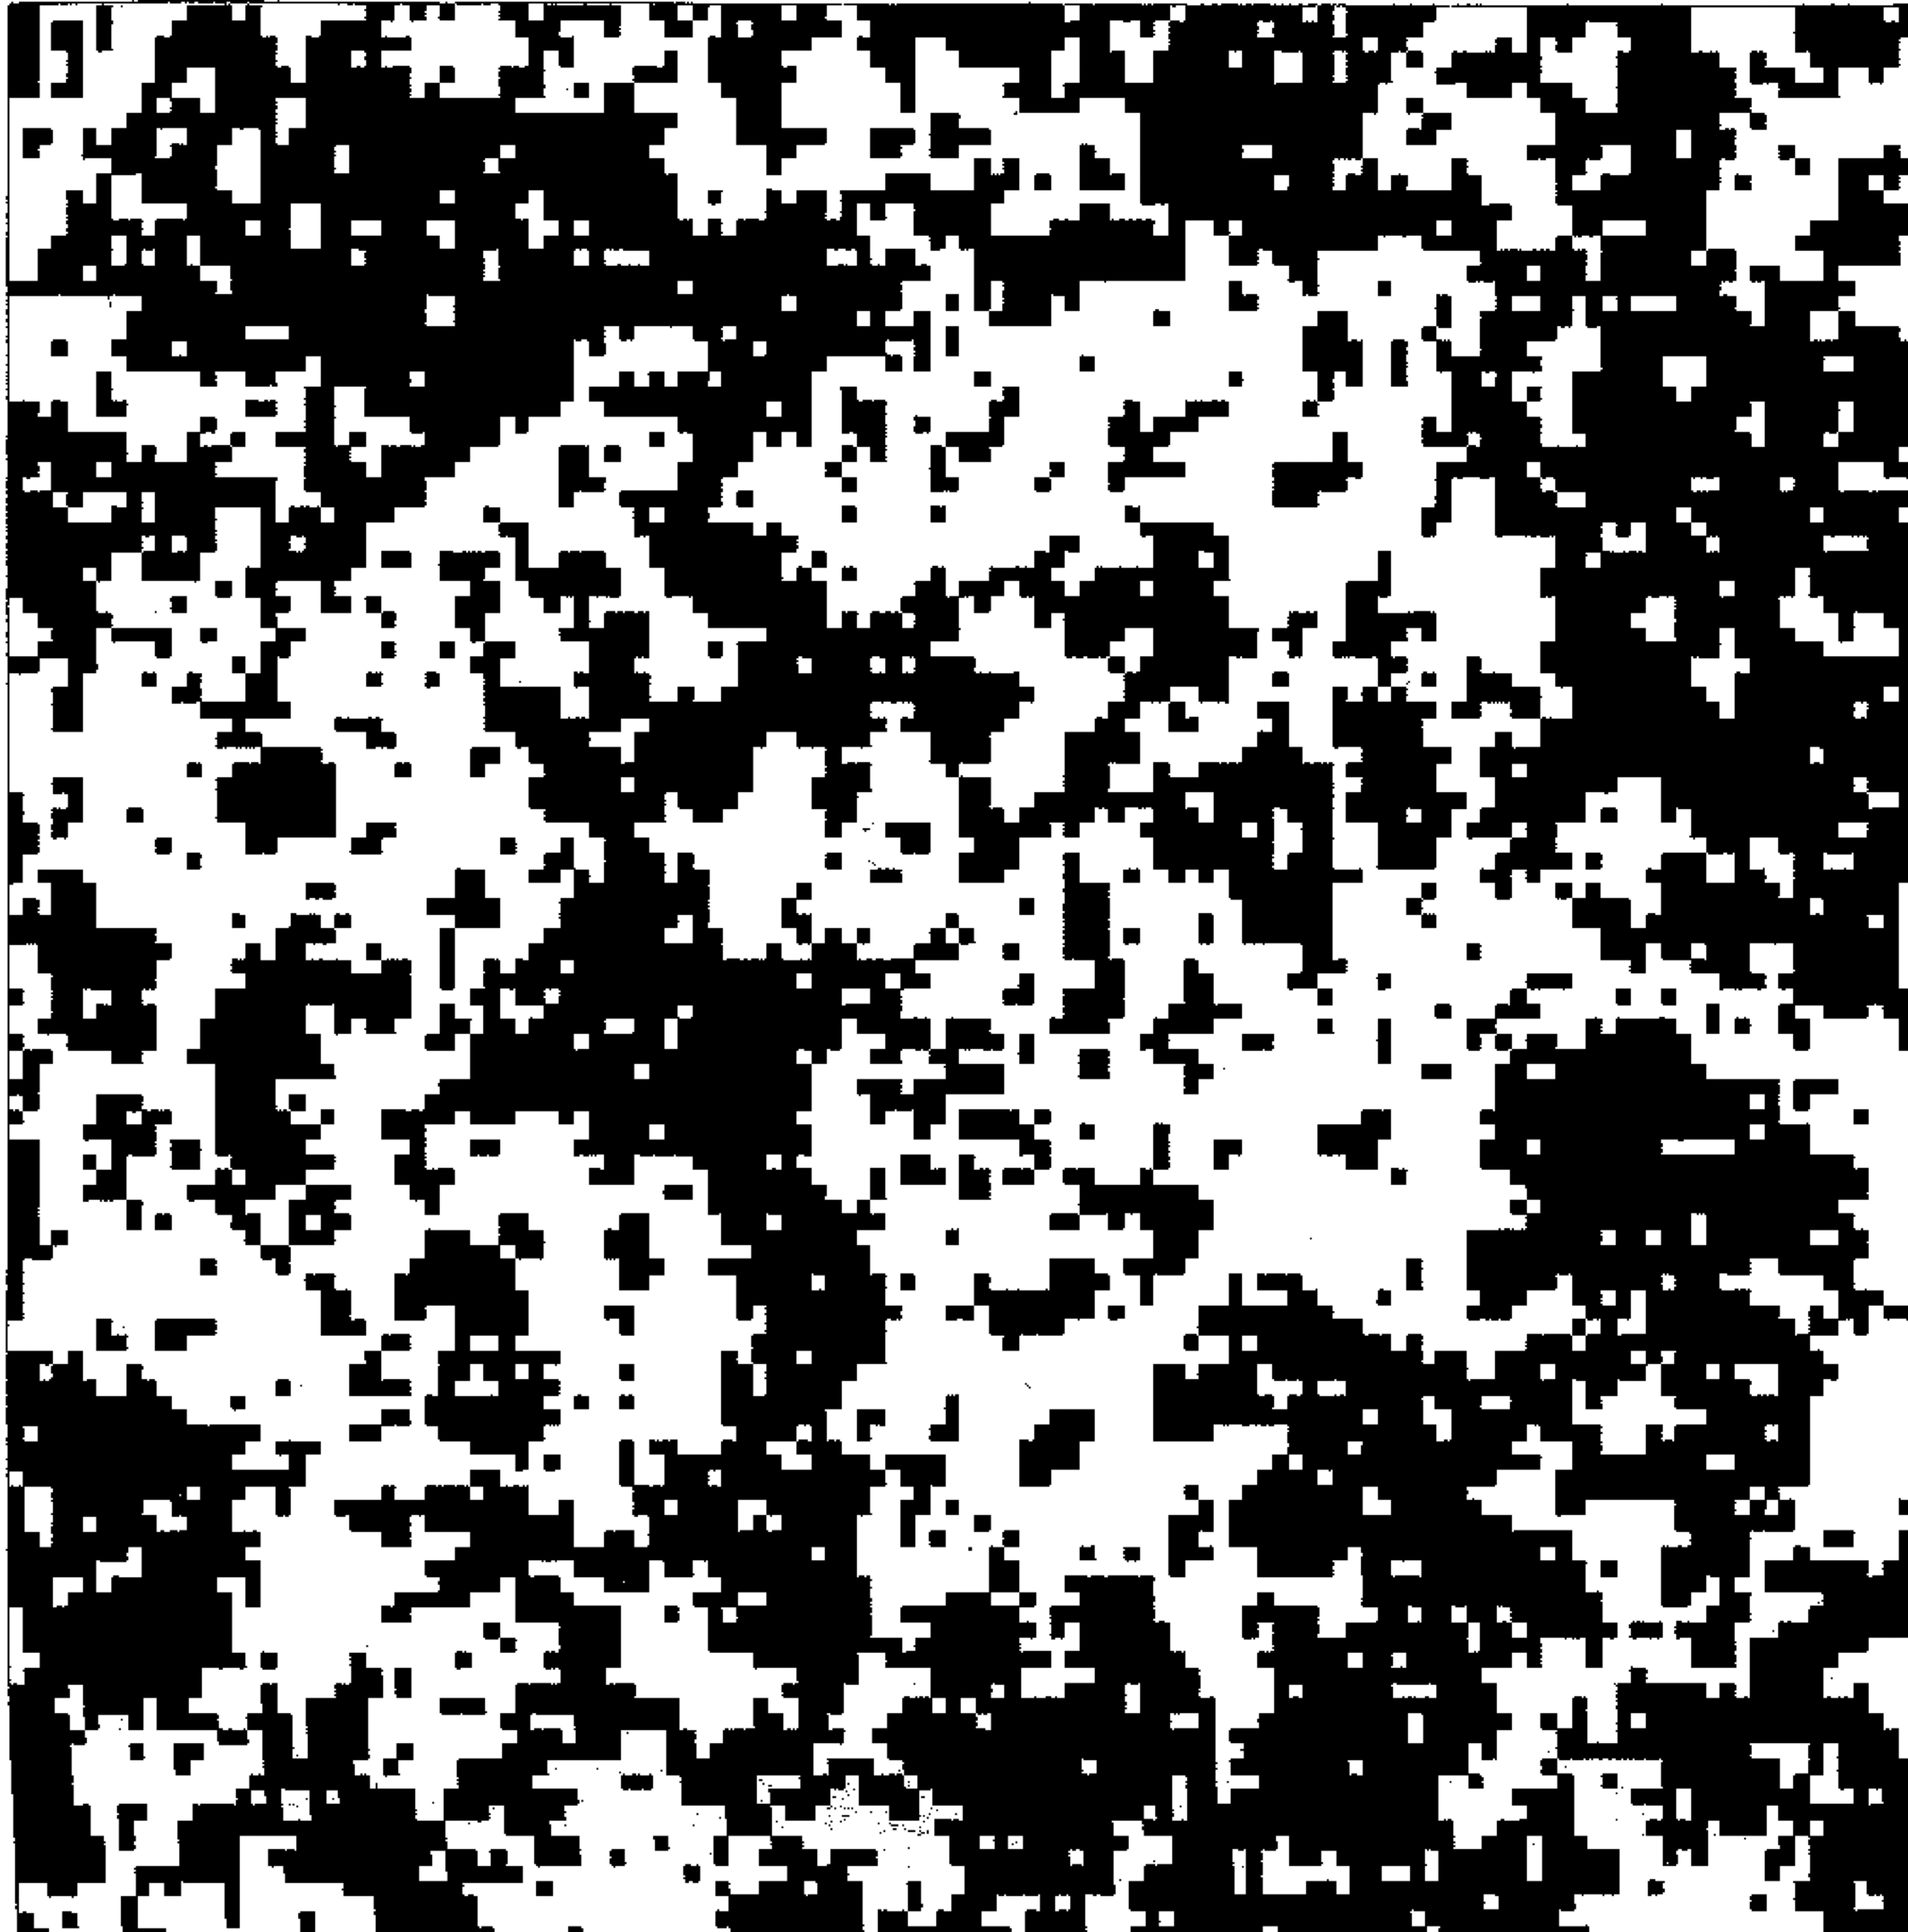
\includegraphics[keepaspectratio]{phase-transitions/Figs/supercrit.png}}

}

\subcaption{\label{fig-ssa}\(T=1.2T_c\)}

\end{minipage}%
%
\begin{minipage}{0.33\linewidth}

\centering{

\pandocbounded{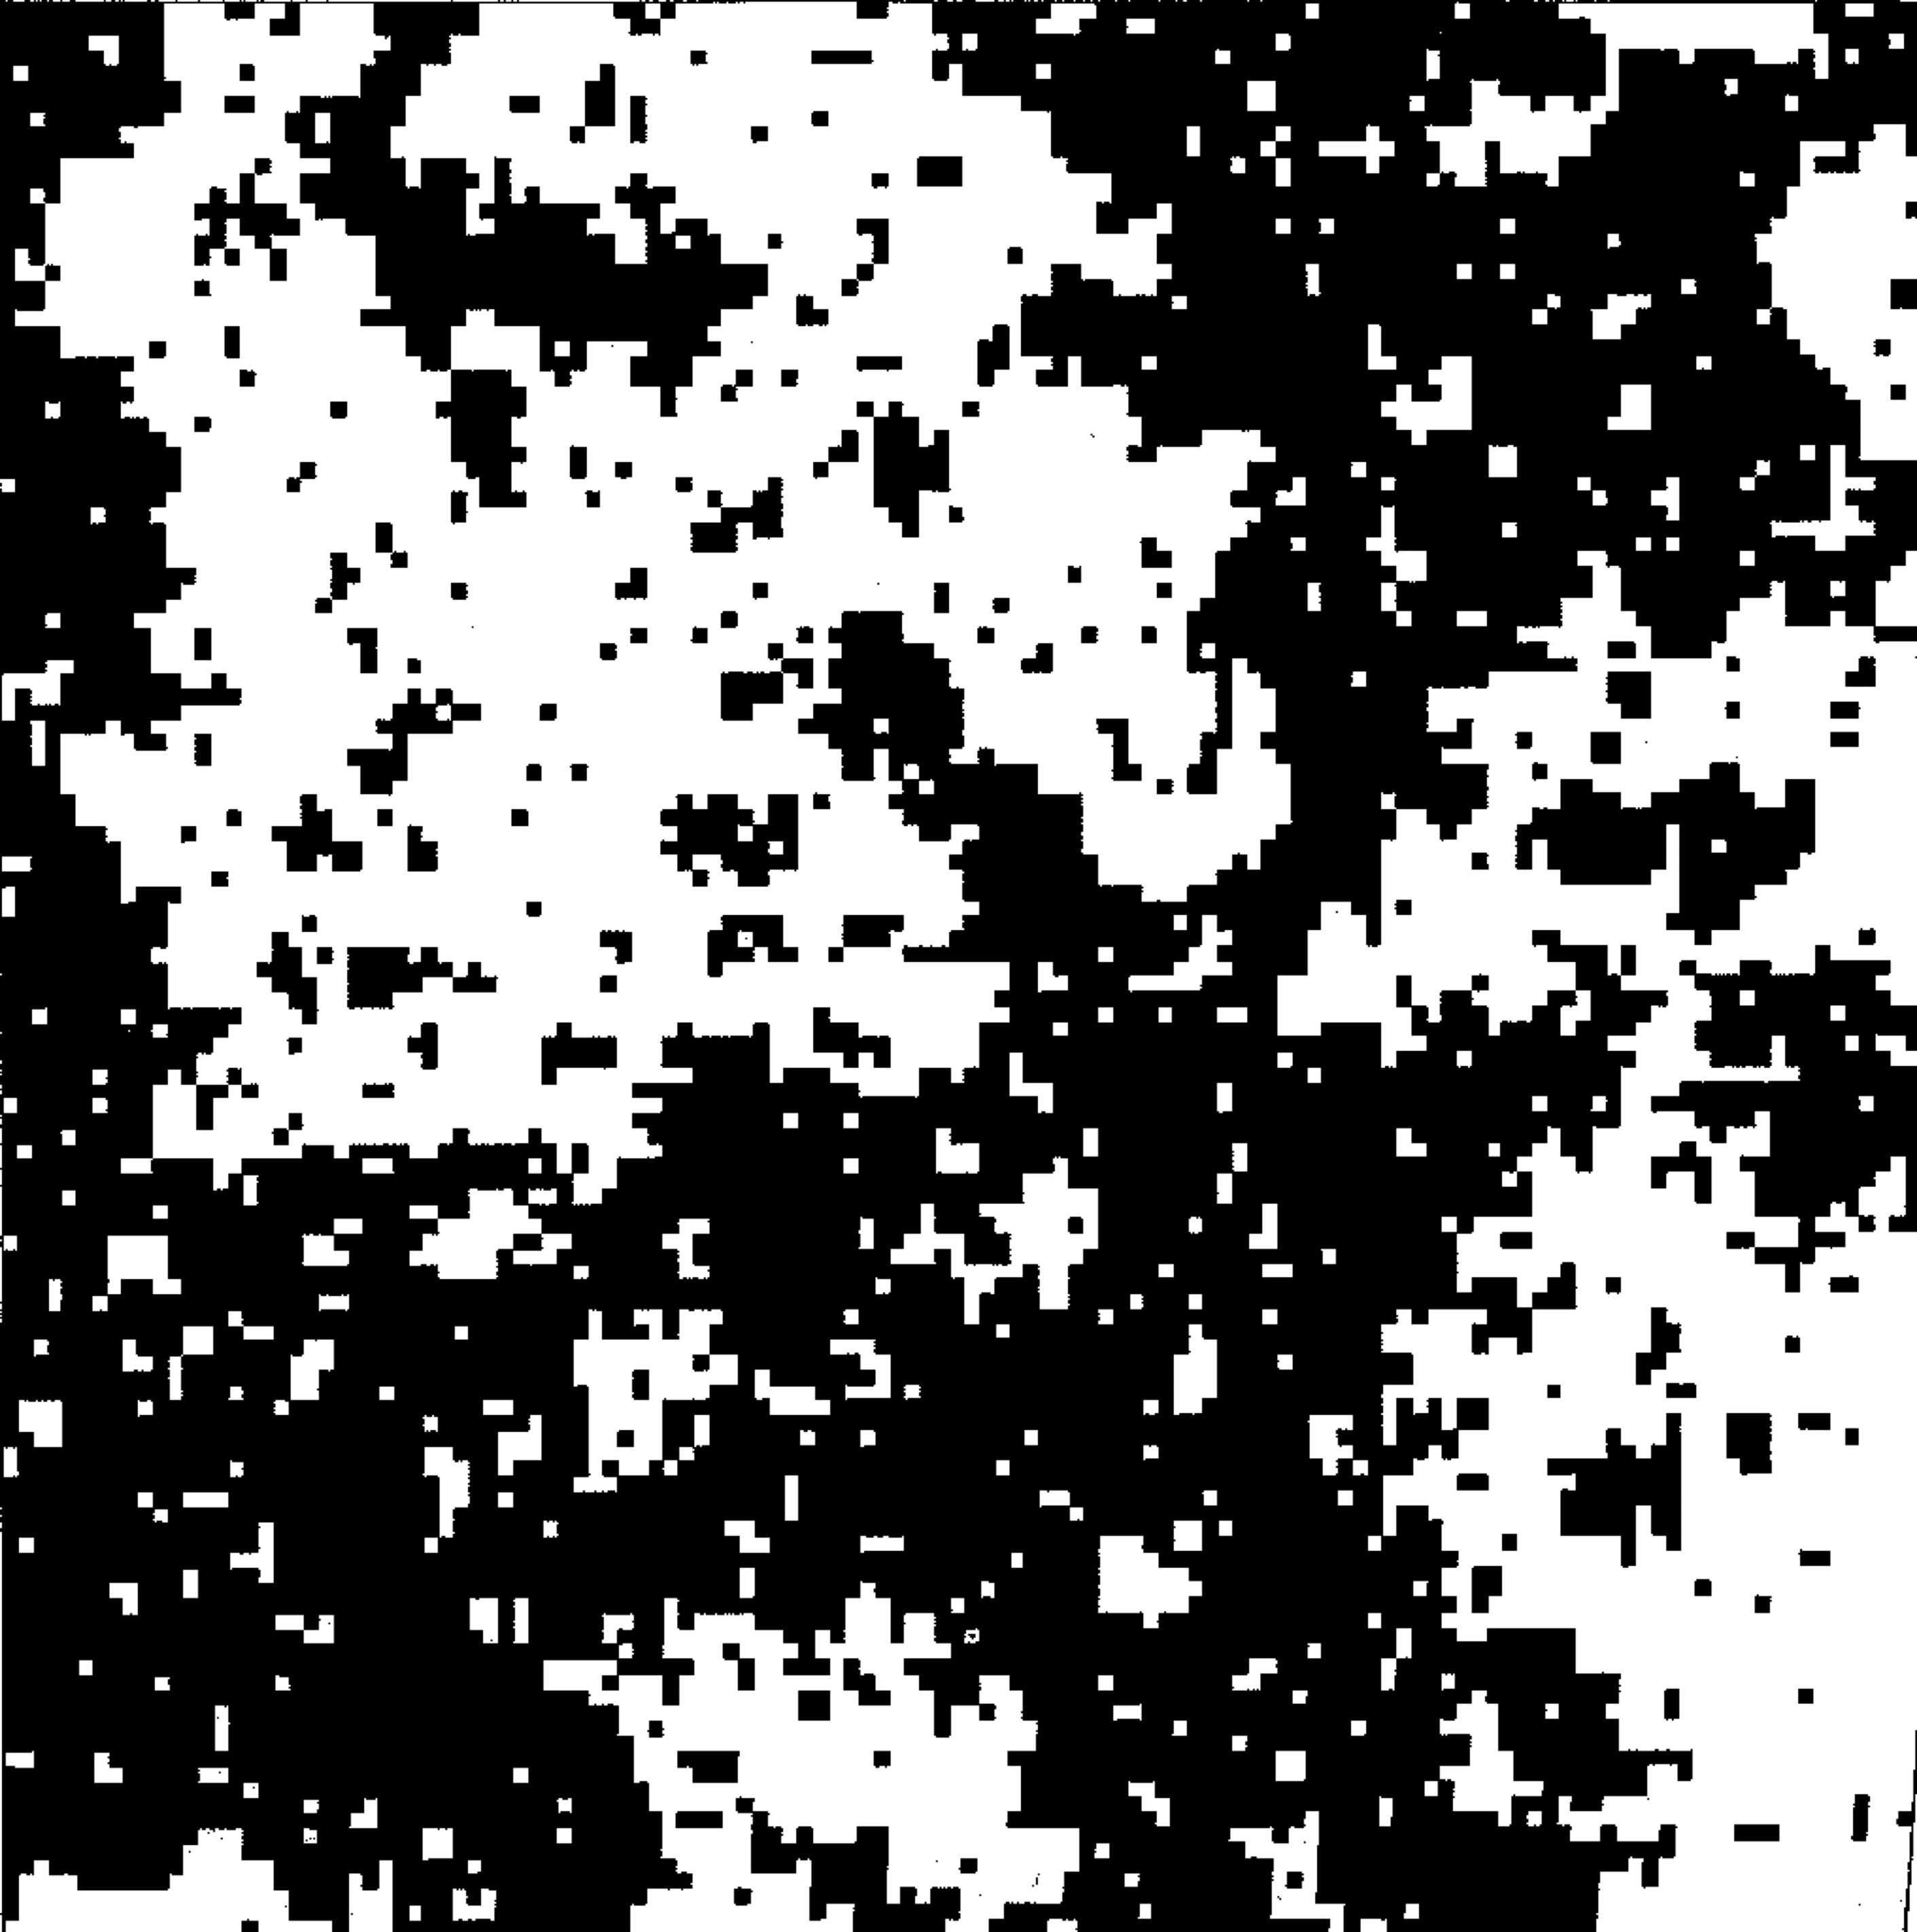
\includegraphics[keepaspectratio]{phase-transitions/Figs/crit.png}}

}

\subcaption{\label{fig-ssb}\(T=T_c\)}

\end{minipage}%
%
\begin{minipage}{0.33\linewidth}

\centering{

\pandocbounded{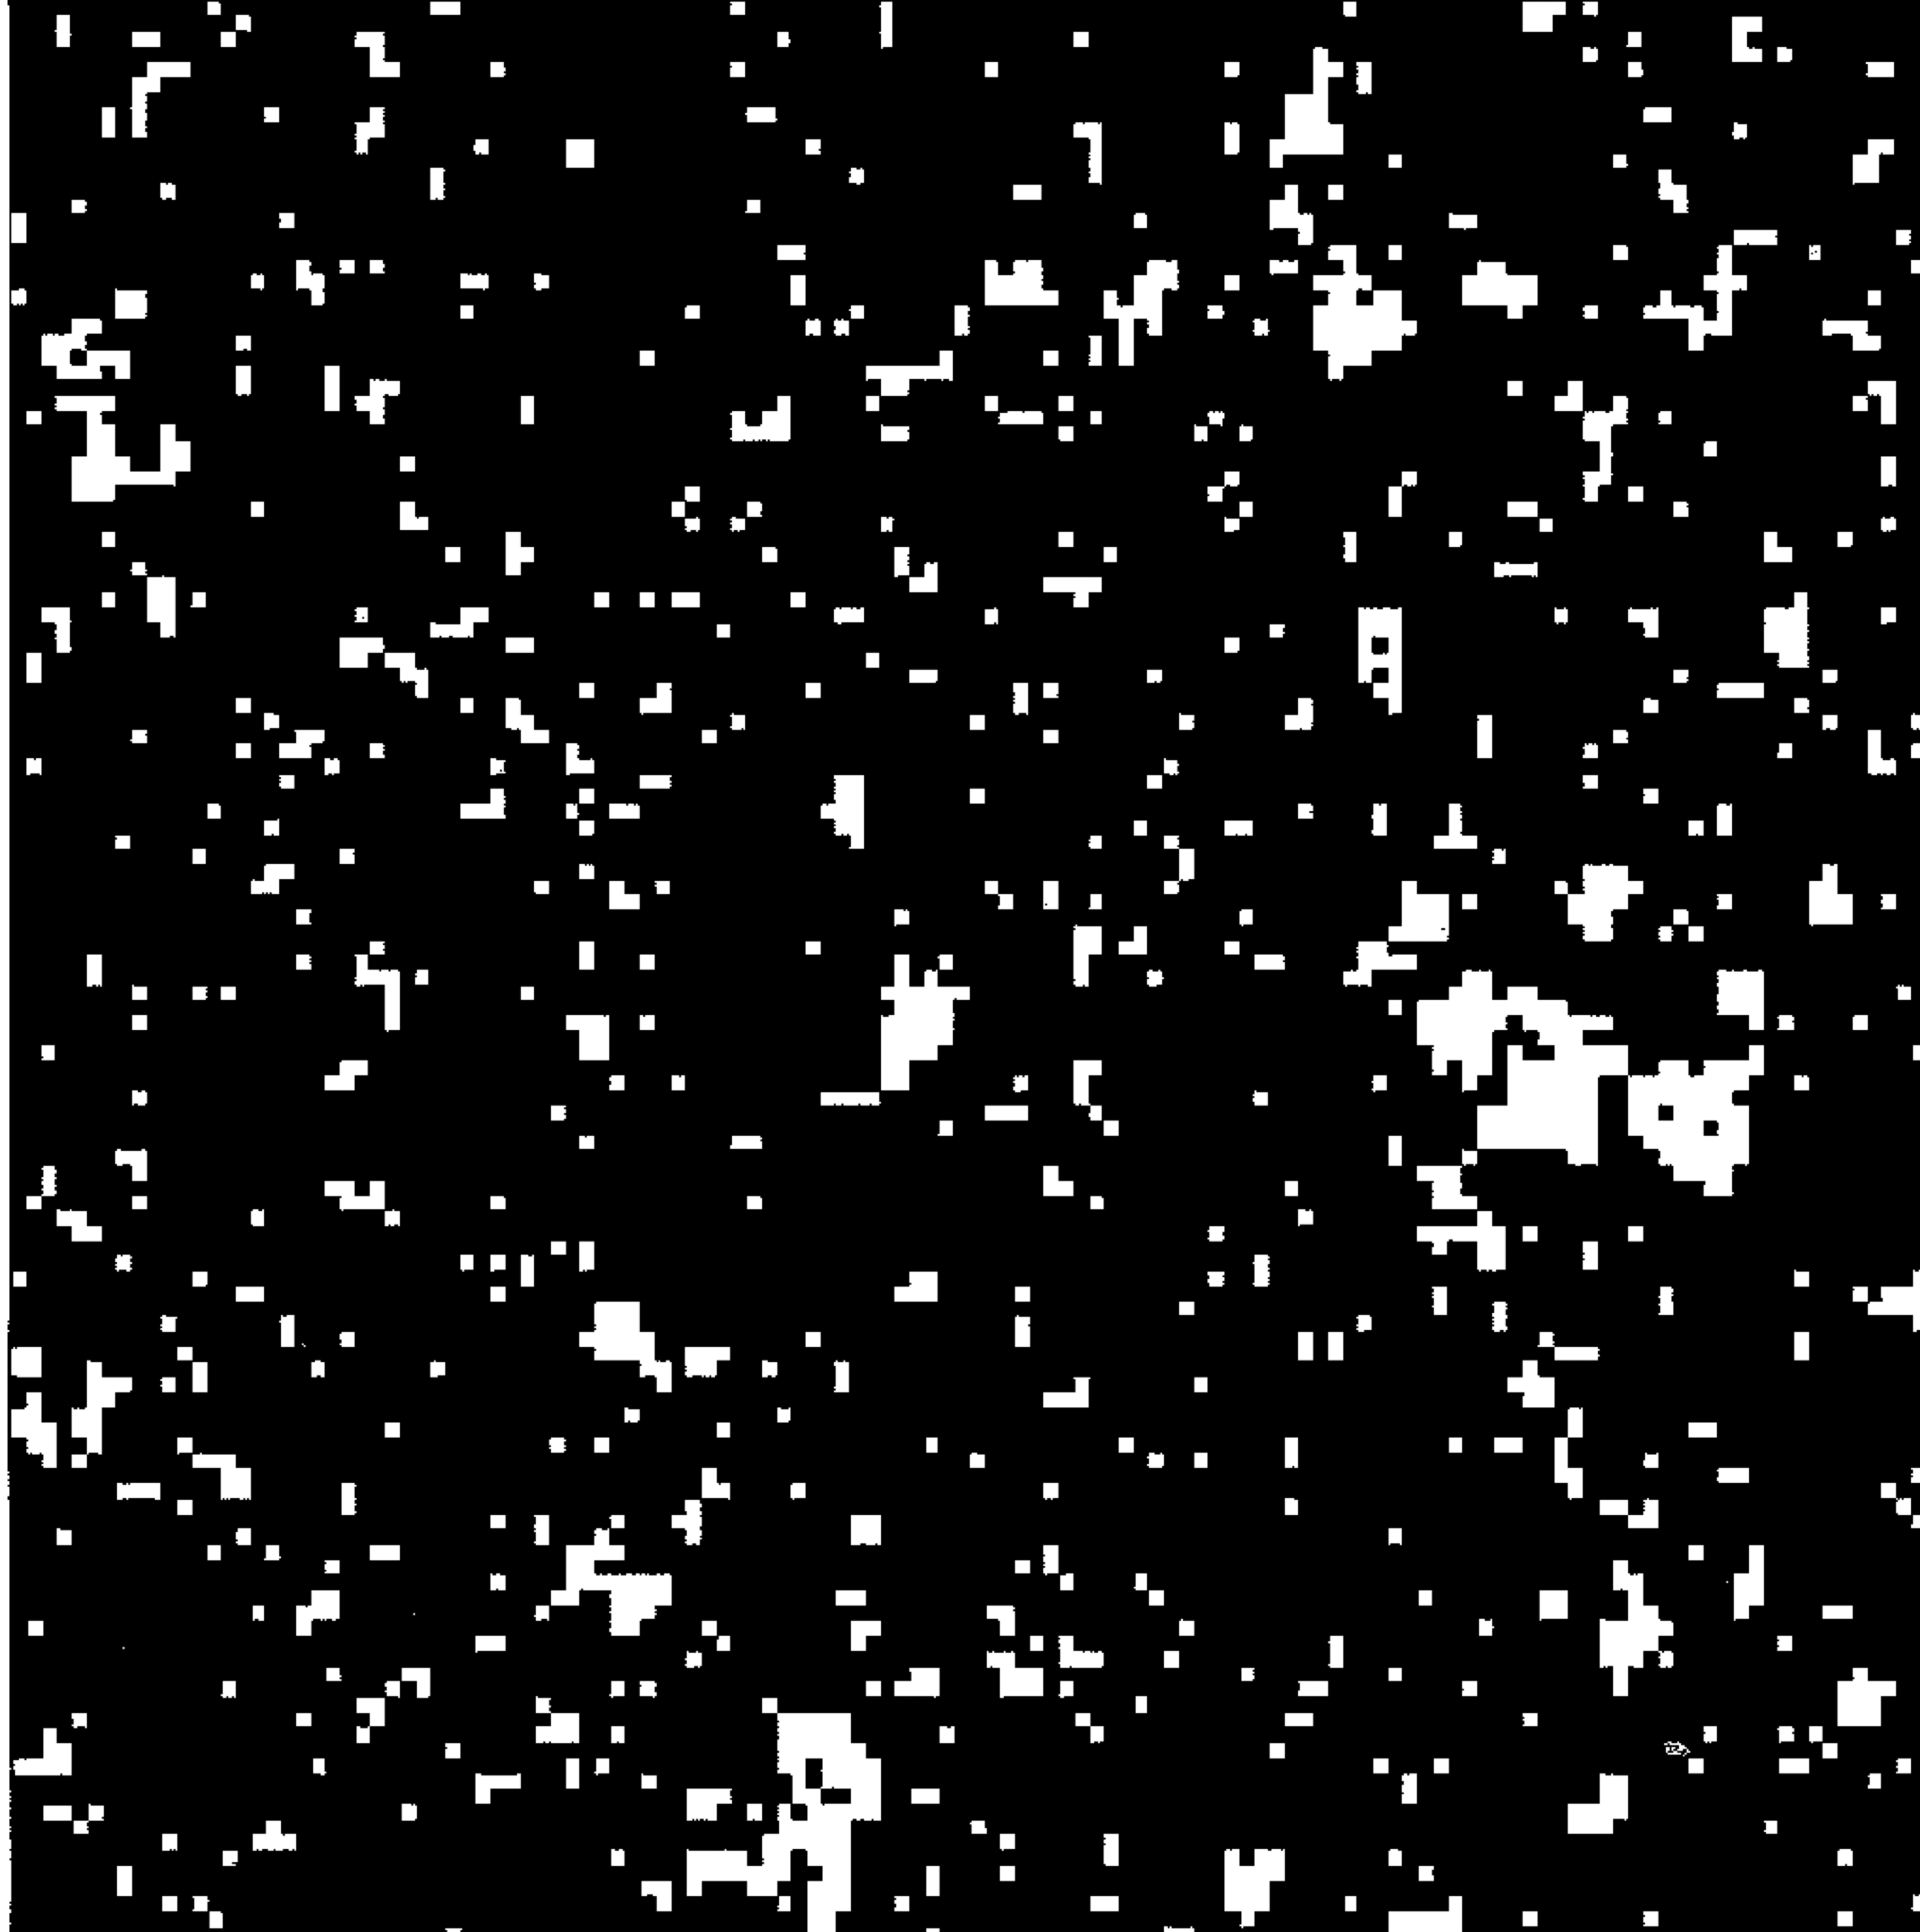
\includegraphics[keepaspectratio]{phase-transitions/Figs/subcrit.png}}

}

\subcaption{\label{fig-ssc}\(T=0.95T_c\)}

\end{minipage}%

\caption{\label{fig-snapshots}Configurations of the 2d Ising model. The
patterns depict typical arrangements of the spins (white=+1, black=−1)
generated in a computer simulation of the Ising model on a square
lattice of \(N=512\) sites, at temperatures (from left to right) of
\(T= 1.2T_c\), \(T=T_c\), and \(T=0.95T_c\). In each case only a portion
of the system containing \(128\) sites in shown. The typical island size
is a measure of the correlation length \(\xi\): the excess of black over
white (below \(T_c\) is a measure of the order parameter.}

\end{figure}%

\href{https://physics.weber.edu/schroeder/software/demos/isingmodel.html}{An
interactive Monte Carlo simulation of the Ising model} demonstrates the
phenomenology, By altering the temperature you will be able to observe
for yourself how the typical spin arrangements change as one traverses
the critical region. Pay particular attention to the configurations near
the critical point. They have very interesting properties. We will
return to them later!

Although the 2-d Ising model may appear at first sight to be an
excessively simplistic portrayal of a real magnetic system, critical
point universality implies that many physical observables such as
critical exponents are not materially influenced by the actual nature of
the microscopic interactions. The Ising model therefore provides a
simple, yet \emph{quantitatively} accurate representation of the
critical properties of a whole range of real magnetic (and indeed fluid)
systems. This universal feature of the model is largely responsible for
its ubiquity in the field of critical phenomena. We shall explore these
ideas in more detail later in the course.

\section{Exact solutions: the one dimensional Ising
chain}\label{exact-solutions-the-one-dimensional-ising-chain}

One might well ask why the 2D Ising model is the simplest model to
exhibit a phase transition. What about the one-dimensional Ising model
(ie. spins on a line)? In fact in one dimension, the Ising model can be
solved exactly. It turns out that the system is paramagnetic for all
\(T>0\), so there is no phase transition at any finite temperature. To
see this, consider the ground state of the system in zero external
field. This will have all spins aligned the same way (say up), and hence
be ferromagnetic. Now consider a configuration with a various ``domain
walls'' dividing spin up and spin down regions:

\begin{figure}

\centering{

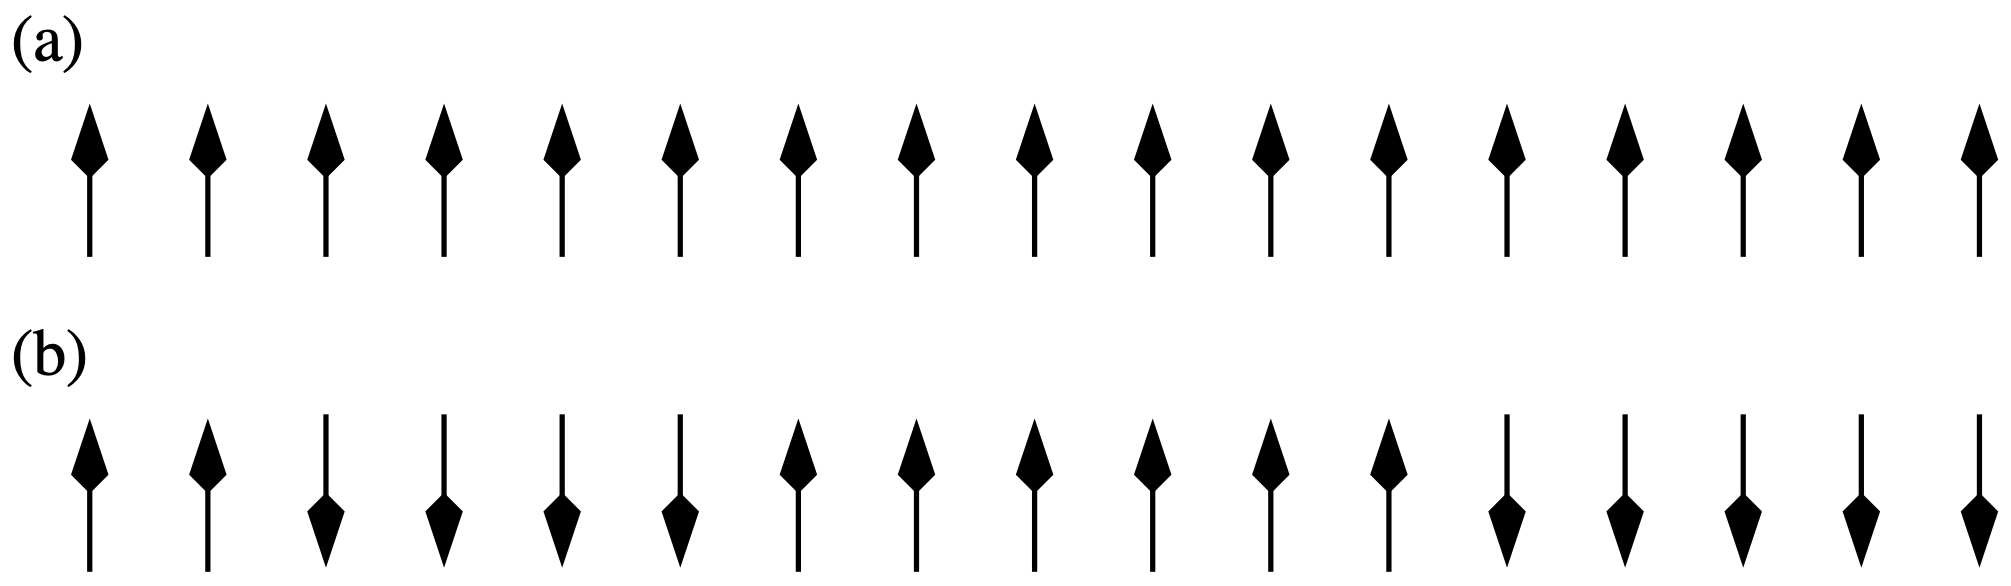
\includegraphics[width=0.8\linewidth,height=\textheight,keepaspectratio]{phase-transitions/Figs/chain.png}

}

\caption{\label{fig-isingchain}(a) Schematic of an Ising chain at
\(T=0\). (b) At a small finite temperature the chain is split into
domains of spins ordered in the same direction. Domains are separated by
notional domain ``walls'', which cost energy \(\Delta=2J\). Periodic
boundary conditions are assumed.}

\end{figure}%

Instead of considering the underlying spin configurations, we shall
describe the system in terms of the statistics of its domain walls. The
energy cost of a wall is \(\Delta = 2J\), independent of position.
Domain walls can occupy the bonds of the lattice, of which there are
\(N-1\). Moreover, the walls are noninteracting, except that you cannot
have two of them on the same bond. (Check through these ideas if you are
unsure.)

In this representation, the partition function involves a count over all
possible domain wall arrangements. Since the domain walls are non
interacting (eg it doesn't cost energy for one to move along the chain)
we can calculate \(Z\) by considering the partition function associated
with a single domain wall being present or absent on some given bond,
and then simply raise to the power of the number of bonds:

\[Z=Z_1^{N-1}\]

where

\[Z_1=e^{\beta J} + e^{\beta (J-\Delta)}=e^{\beta J}(1+e^{-\beta\Delta})\]
is the domain wall partition function for a single bond and represent
the sum over the two possible states: domain wall absent or present.
Then the free energy per bond of the system is

\[\beta f\equiv \beta F/(N-1)=-\ln Z_1=-\beta J-\ln(1+e^{-\beta\Delta})\]

The first term on the RHS is simply the energy per spin of the
ferromagnetic (ordered) phase, while the second term arises from the
free energy of domain walls. Clearly for any finite temperature (ie. for
\(\beta<\infty\)), this second term is finite and negative. Hence the
free energy will always be lowered by having a finite concentration of
domain walls in the system. Since these domain walls disorder the
system, leading to a zero average magnetisation, the 1D system is
paramagnetic for all finite temperatures. \emph{Exercise}: Explain why
this argument works only in 1D.

The animation below lets you see qualitatively how the typical number of
domain walls varies with temperature. If you'd lke to explore more
quantitatively, a python code performing a Monte Carlo simulation is
available. You will learn about Monte Carlo simulation in the coursework
and in later parts of the course.

\begin{Shaded}
\begin{Highlighting}[]
\CommentTok{\#Monte Carlo simulation of the 1d Ising chain with periodic bounary conditions}
\ImportTok{import}\NormalTok{ numpy }\ImportTok{as}\NormalTok{ np}
\ImportTok{import}\NormalTok{ matplotlib.pyplot }\ImportTok{as}\NormalTok{ plt}
\ImportTok{from}\NormalTok{ matplotlib.animation }\ImportTok{import}\NormalTok{ FuncAnimation}
\ImportTok{from}\NormalTok{ matplotlib.widgets }\ImportTok{import}\NormalTok{ Slider}

\CommentTok{\# Number of spins}
\NormalTok{N }\OperatorTok{=} \DecValTok{20} 

\CommentTok{\# Initialize spins (+1 or {-}1)}
\NormalTok{spins }\OperatorTok{=}\NormalTok{ np.random.choice([}\OperatorTok{{-}}\DecValTok{1}\NormalTok{, }\DecValTok{1}\NormalTok{], size}\OperatorTok{=}\NormalTok{N)}

\CommentTok{\# Initial temperature}
\NormalTok{T }\OperatorTok{=} \FloatTok{2.0}

\CommentTok{\# Set up figure and axis for the spins}
\NormalTok{fig, ax }\OperatorTok{=}\NormalTok{ plt.subplots(figsize}\OperatorTok{=}\NormalTok{(}\DecValTok{10}\NormalTok{, }\DecValTok{2}\NormalTok{))}
\NormalTok{plt.subplots\_adjust(bottom}\OperatorTok{=}\FloatTok{0.25}\NormalTok{)  }\CommentTok{\# make room for slider}
\NormalTok{ax.set\_xlim(}\OperatorTok{{-}}\FloatTok{0.5}\NormalTok{, N }\OperatorTok{{-}} \FloatTok{0.5}\NormalTok{)}
\NormalTok{ax.set\_ylim(}\OperatorTok{{-}}\DecValTok{1}\NormalTok{, }\DecValTok{1}\NormalTok{)}
\NormalTok{ax.axis(}\StringTok{\textquotesingle{}off\textquotesingle{}}\NormalTok{)}

\CommentTok{\# Create text objects for each spin}
\NormalTok{texts }\OperatorTok{=}\NormalTok{ []}
\ControlFlowTok{for}\NormalTok{ i }\KeywordTok{in} \BuiltInTok{range}\NormalTok{(N):}
\NormalTok{    arrow }\OperatorTok{=} \StringTok{\textquotesingle{}↑\textquotesingle{}} \ControlFlowTok{if}\NormalTok{ spins[i] }\OperatorTok{==} \DecValTok{1} \ControlFlowTok{else} \StringTok{\textquotesingle{}↓\textquotesingle{}}
\NormalTok{    t }\OperatorTok{=}\NormalTok{ ax.text(i, }\DecValTok{0}\NormalTok{, arrow, fontsize}\OperatorTok{=}\DecValTok{24}\NormalTok{, ha}\OperatorTok{=}\StringTok{\textquotesingle{}center\textquotesingle{}}\NormalTok{, va}\OperatorTok{=}\StringTok{\textquotesingle{}center\textquotesingle{}}\NormalTok{)}
\NormalTok{    texts.append(t)}

\KeywordTok{def}\NormalTok{ update(frame):}
    \CommentTok{"""Perform Metropolis updates over all spins, then refresh display."""}
    \KeywordTok{global}\NormalTok{ spins, T}
    \ControlFlowTok{for}\NormalTok{ \_ }\KeywordTok{in} \BuiltInTok{range}\NormalTok{(N):}
\NormalTok{        i }\OperatorTok{=}\NormalTok{ np.random.randint(N)}
\NormalTok{        left }\OperatorTok{=}\NormalTok{ spins[(i }\OperatorTok{{-}} \DecValTok{1}\NormalTok{) }\OperatorTok{\%}\NormalTok{ N]}
\NormalTok{        right }\OperatorTok{=}\NormalTok{ spins[(i }\OperatorTok{+} \DecValTok{1}\NormalTok{) }\OperatorTok{\%}\NormalTok{ N]}
\NormalTok{        deltaE }\OperatorTok{=} \DecValTok{2} \OperatorTok{*}\NormalTok{ spins[i] }\OperatorTok{*}\NormalTok{ (left }\OperatorTok{+}\NormalTok{ right)}
        \CommentTok{\# Metropolis criterion ensures configurations appear with the correct Boltzmann probability}
        \ControlFlowTok{if}\NormalTok{ deltaE }\OperatorTok{\textless{}} \DecValTok{0} \KeywordTok{or}\NormalTok{ np.random.rand() }\OperatorTok{\textless{}}\NormalTok{ np.exp(}\OperatorTok{{-}}\NormalTok{deltaE }\OperatorTok{/}\NormalTok{ T):}
\NormalTok{            spins[i] }\OperatorTok{*=} \OperatorTok{{-}}\DecValTok{1}
    \CommentTok{\# Update arrows on screen}
    \ControlFlowTok{for}\NormalTok{ idx, t }\KeywordTok{in} \BuiltInTok{enumerate}\NormalTok{(texts):}
\NormalTok{        t.set\_text(}\StringTok{\textquotesingle{}↑\textquotesingle{}} \ControlFlowTok{if}\NormalTok{ spins[idx] }\OperatorTok{==} \DecValTok{1} \ControlFlowTok{else} \StringTok{\textquotesingle{}↓\textquotesingle{}}\NormalTok{)}
    \ControlFlowTok{return}\NormalTok{ texts}

\CommentTok{\# Create the animation with caching disabled and blit turned off}
\NormalTok{ani }\OperatorTok{=}\NormalTok{ FuncAnimation(}
\NormalTok{    fig,}
\NormalTok{    update,}
\NormalTok{    interval}\OperatorTok{=}\DecValTok{200}\NormalTok{,}
\NormalTok{    blit}\OperatorTok{=}\VariableTok{False}\NormalTok{,}
\NormalTok{    cache\_frame\_data}\OperatorTok{=}\VariableTok{False}
\NormalTok{)}

\CommentTok{\# Add a temperature slider}
\NormalTok{ax\_T }\OperatorTok{=}\NormalTok{ plt.axes([}\FloatTok{0.2}\NormalTok{, }\FloatTok{0.1}\NormalTok{, }\FloatTok{0.6}\NormalTok{, }\FloatTok{0.03}\NormalTok{], facecolor}\OperatorTok{=}\StringTok{\textquotesingle{}lightgray\textquotesingle{}}\NormalTok{)}
\NormalTok{slider\_T }\OperatorTok{=}\NormalTok{ Slider(ax\_T, }\StringTok{\textquotesingle{}Temperature T\textquotesingle{}}\NormalTok{, }\FloatTok{0.1}\NormalTok{, }\FloatTok{5.0}\NormalTok{, valinit}\OperatorTok{=}\NormalTok{T)}

\KeywordTok{def}\NormalTok{ on\_T\_change(val):}
    \CommentTok{"""Callback to update T when the slider changes."""}
    \KeywordTok{global}\NormalTok{ T}
\NormalTok{    T }\OperatorTok{=}\NormalTok{ val}

\NormalTok{slider\_T.on\_changed(on\_T\_change)}

\CommentTok{\# Show the plot (ani is kept in scope so it won\textquotesingle{}t be deleted)}
\NormalTok{plt.show()}
\end{Highlighting}
\end{Shaded}

\phantomsection\label{ising}

Temperature T =

2.0

\subsection{More general 1D spins systems: transfer matrix
method}\label{more-general-1d-spins-systems-transfer-matrix-method}

Generally speaking one-dimensional systems lend themselves to a degree
of analytic tractability not found in most higher dimensional models.
Indeed for the case of a 1-d assembly of \(N\) spins each having \(m\)
discrete energy states, and in the presence of a magnetic field, it is
possible to reduce the evaluation of the partition function to the
calculation of the eigenvalues of a matrix--the so called transfer
matrix.

Let us start by assuming that the assembly has cyclic boundary
conditions, then the total energy of configuration \(\{s\}\) is \[
\begin{aligned}
H(\{s\})=&-\sum_{i=1}^N (J s_i s_{i+1}+Hs_i)\\
\:=&-\sum_{i=1}^N (J s_i s_{i+1}+H(s_i+s_{i+1})/2)\\
\:=&\sum_{i=1}^N E(s_i,s_{i+1})
\end{aligned}
\]

where we have defined
\(E(s_i,s_{i+1})=-J s_i s_{i+1}-H(s_i+s_{i+1})/2\).

Now the partition function may be written

\begin{equation}\phantomsection\label{eq-Vs}{\begin{aligned}
Z_N =& \sum_{\{s\}}\exp\left(-\beta H(\{s\})\right)\nonumber \\
 =&\sum_{\{s\}}\exp\left(-\beta[E(s_1,s_2)+E(s_2,s_3)+....E(s_N,s_1)]\right) \nonumber\\
 =&\sum_{\{s\}}\exp\left(-\beta E(s_1,s_2)\right)\exp\left(-\beta E(s_2,s_3)\right)....\exp\left(-\beta E(s_N,s_1)\right) \nonumber\\
=&\sum_{i,j,...,l=1}^m V_{ij}V_{jk}...V_{li} 
\end{aligned}}\end{equation}

where the \(V_{ij}=\exp(-\beta E_{ij})\) are elements of an
\(m \times m\) matrix \({\bf V}\), known as the transfer matrix
(\(i,j,k\) etc are dummy indices that run over the matrix elements). You
should see that the sum over the product of matrix elements picks up all
the terms in the partition function and therefore Equation~\ref{eq-Vs}
is an alternative way of writing the partition function.

The reason it is useful to transform to a matrix representation is that
it transpires that the sum over the product of matrix elements in
Equation~\ref{eq-Vs} is simply just the trace of \({\bf V}^N\) (check
this yourself for a short periodic chain), given by the sum of its
eigenvalues:-

\[Z_N=\lambda_1^N+\lambda_2^N+...\lambda_m^N\] For very large \(N\),
this expression simplifies further because the largest eigenvalue
\(\lambda_1\) dominates the behaviour since \((\lambda_2/\lambda_1)^N\)
vanishes as \(N\rightarrow \infty\). Consequently in the thermodynamic
limit one may put \(Z_N=\lambda_1^N\) and the problem reduces to
identifying the largest eigenvalue of the transfer matrix.

Specializing to the case of the simple Ising model in the presence of an
applied field \(H\), the transfer matrix takes the form

\[{\bf V}(H)=\left(
\begin{array}{cc}
e^{\beta(J+H)} & e^{-\beta J} \\
e^{-\beta J}   & e^{\beta(J-H)}
\end{array} \right)\]

This matrix has two eigenvalues which can be readily calculated in the
usual fashion as the roots of the characteristic polynomial
\(|{\bf V}-\lambda{\bf I}|\). They are

\[\lambda_{\pm}=e^{\beta J}\cosh(\beta H) \pm \sqrt{e^{2\beta J}\sinh^2\beta H+e^{-2\beta J}}.\]

Hence the free energy per spin \(f=-k_BT\ln \lambda_+\) is

\[f=-k_BT\ln \left[e^{\beta J}\cosh(\beta H) + \sqrt{e^{2\beta J}\sinh^2\beta H+e^{-2\beta J}}\right].\]

The Ising model in 2D can also be solved exactly, as was done by Lars
Onsager in 1940. The solution is extremely complicated and is regarded
as one of the pinnacles of statistical mechanics. In 3D no exact
solution is known.

\chapter{Mean field theory and perturbation
schemes}\label{mean-field-theory-and-perturbation-schemes}

Of the wide variety of models of interest to the critical point
theorist, the majority have shown themselves intractable to direct
analytic (pen and paper) assault. In a very limited number of instances
models have been solved exactly, yielding the phase coexistence
parameters, critical exponents and the critical temperature. The 2-d
spin-\(\frac{1}{2}\) Ising model is certainly the most celebrated such
example, its principal critical exponents are found to be
\(\beta=\frac{1}{8}, \nu=1, \gamma=\frac{7}{4}\). Its critical
temperature is \(-2J/\ln(\sqrt{2}-1)\approx 2.269J\). Unfortunately such
solutions rarely afford deep insight to the general framework of
criticality although they do act as an invaluable test-bed for new and
existing theories.

The inability to solve many models exactly often means that one must
resort to approximations. One such approximation scheme is mean field
theory.

\section{Mean field solution of the Ising model}\label{sec:mfising}

Let us look for a mean field expression for the free energy of the Ising
model whose Hamiltonian is given in Equation~\ref{eq-ising} . Write

\[s_i=\langle s_i\rangle+(s_i-\langle s_i\rangle)=m+(s_i-m)=m+\delta s_i\]

Then \begin{equation}\phantomsection\label{eq-mfa}{\begin{aligned}
{\cal H}_I=&-J\sum_{<i,j>}[m+(s_i-m)][m+(s_j-m)]-H\sum_i s_i\nonumber\\
=&-J\sum_{<i,j>}[m^2+m(s_i-m)+m(s_j-m)+\delta s_i\delta s_j]-H\sum_i s_i\nonumber\\
=&-J\sum_{i}(qms_i-qm^2/2)-H\sum_i s_i-J\sum_{<i,j>}\delta s_i\delta s_j 
\end{aligned}}\end{equation} where in the last line we have used the
fact that when for each site \(i\) we perform the sum \(\sum_{<i,j>}\)
over bonds of a quantity which is independent of \(s_j\), then the
result is just the number of bonds per site times that quantity. Since
the number of bonds on a lattice of \(N\) sites of coordination \(q\) is
\(Nq/2\) (because each bond is shared between two sites), there are
therefore \(q/2\) bonds per site.

Now the mean field approximation is to ignore the last term in the last
line of Equation~\ref{eq-mfa} giving the configurational energy as

\[
{\cal H}_{mf}=-\sum_{i}H_{mf}s_i+NqJm^2/2
\] with \(H_{mf}\equiv qJm+ H\) the ``mean field'' seen by spin \(s_i\).
As all the spins are decoupled (independent) in this approximation we
can write down the partition function, which follows by taking the
partition function for a single spin (by summing the Boltzmann factor
for \(s_i=\pm 1\)) and raising to the power \(N\) to find

\[
Z=e^{-\beta qJm^2N/2}[2\cosh(\beta(qJm+H))]^N
\]

The free energy follows as

\[F(m)=NJqm^2/2-Nk_BT\ln[2\cosh(\beta (qJm+H)]\:.\]

and the magnetisation as

\[
m=-\frac{1}{N}\frac{\partial F}{\partial H}=\tanh(\beta(qJm+H))
\]

To find \(m(H,T)\), we must numerically solve this last equation self
consistently.

Note that we can obtain \(m\) in a different way. Consider some arbitary
spin, \(s_i\) say. Then this spin has an energy \({\cal H}_{mf}(s_i)\).
Considering this energy for both cases \(s_i=\pm 1\) and the probability
\(p(s_i)=e^{-\beta{\cal H}_{mf}(s_i)}/Z\) of each, we have that

\[\langle s_i\rangle=\sum_{s_i=\pm 1}s_ip(s_i)\] but for consistancy,
\(\langle s_i\rangle=m\). Thus

\begin{equation}\phantomsection\label{eq-mfmag}{
\begin{aligned}
m & = \sum_{s_i=\pm 1}s_ip(s_i)\nonumber\\
 \: & = \frac{e^{\beta(qJm+H)}-e^{\beta(qJm+H)}} {e^{\beta(qJm+H)}+e^{-\beta(qJm+H)}}\nonumber\\
 \: & = \tanh(\beta(qJm+H))
\end{aligned}}\end{equation} as before.

\section{Spontaneous symmetry breaking}\label{sec-breaking}

\begin{figure}

\centering{

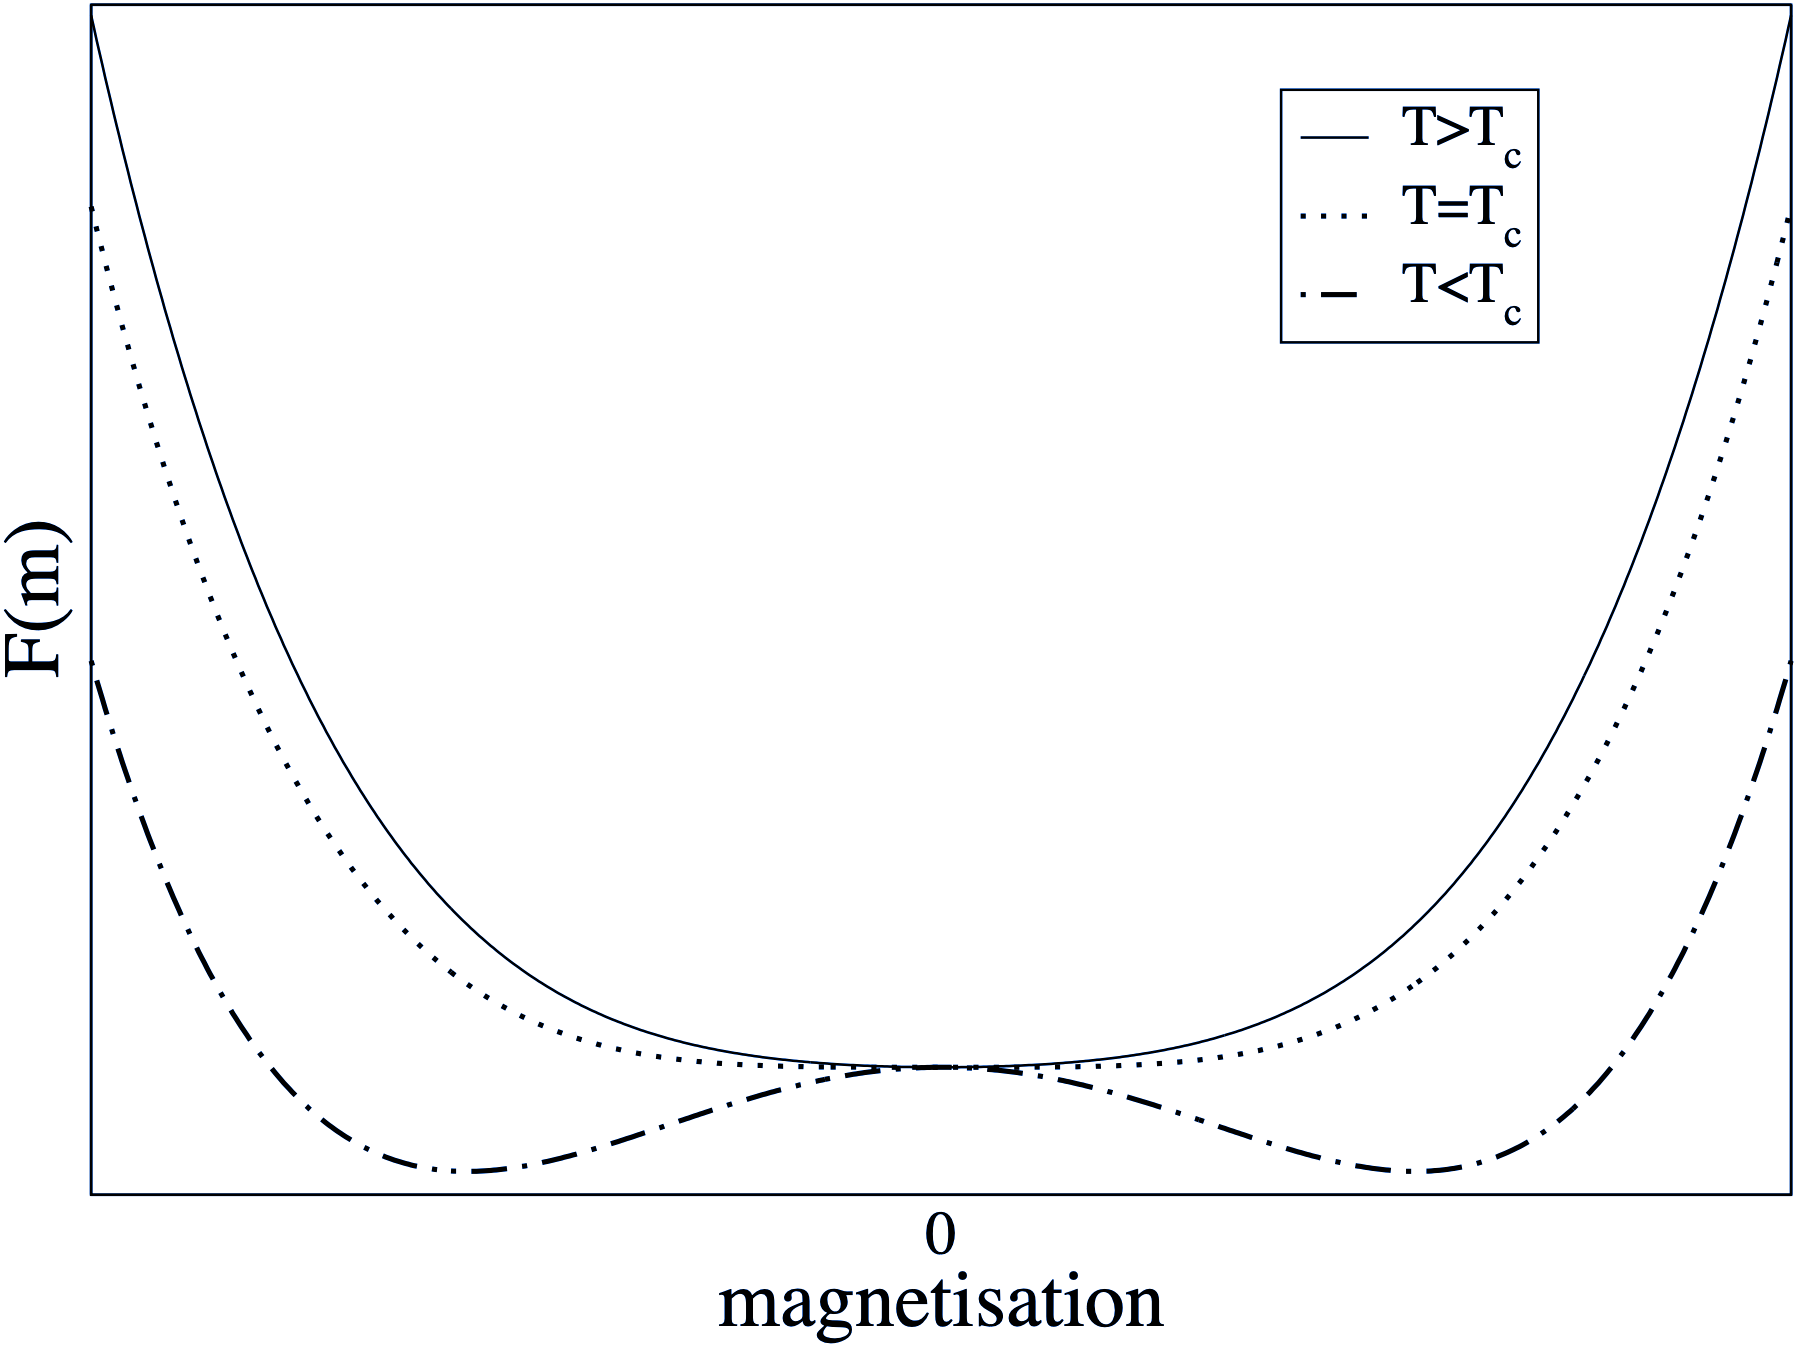
\includegraphics[width=0.7\linewidth,height=\textheight,keepaspectratio]{phase-transitions/Figs/freeenergy_color.png}

}

\caption{\label{fig-freeenergy}Schematic of the form of the free energy
for a critical, subcritical and supercritical temperature}

\end{figure}%

This mean field analysis reveals what is happening in the Ising model
near the critical temperature \(T_c\). Figure~\ref{fig-freeenergy} shows
sketches for \(\beta F(m)/N\) as a function of temperature, where for f
simplicity we restrict attention to \(H=0\). In this case \(F(m)\) is
symmetric in \(m\), Moreover, at high \(T\), the entropy dominates and
there is a single minimum in \(F(m)\) at \(m=0\). As \(T\) is lowered,
there comes a point (\(T=T_c=qJ/k_B\)) where the curvature of \(F(m)\)
at the origin changes sign; precisely at this point

\[\frac{\partial^2 F}{\partial m^2}=0.\] At lower temperature, there are
instead two minima at nonzero \(m=\pm m^\star\), where the
\emph{equilibrium magnetisation} \(m^\star\) is the positive root
(calculated explicitly below) of

\[m^\star=\tanh(\beta Jqm^\star)= \tanh(\frac{m^\star T_c}{T})\] The
point \(m=0\) which remains a root of this equation, is clearly an
unstable point for \(T<T_c\) (since \(F\) has a maximum there).

This is an example of spontaneous symmetry breaking. In the absence of
an external field, the Hamiltonian (and therefore the free energy) is
symmetric under \(m\to -m\). Accordingly, one might expect the actual
state of the system to also show this symmetry. This is true at high
temperature, but spontaneously breaks down at low ones. Instead there
are a pair of ferromagnetic states (spins mostly up, or spins mostly
down) which -- by symmetry-- have the same free energy, lower than the
unmagnetized state.

\section{Phase diagram}\label{phase-diagram}

The resulting zero-field magnetisation curve \(m(T,H=0)\) looks like
Figure~\ref{fig-isingmag}.

\begin{figure}

\centering{

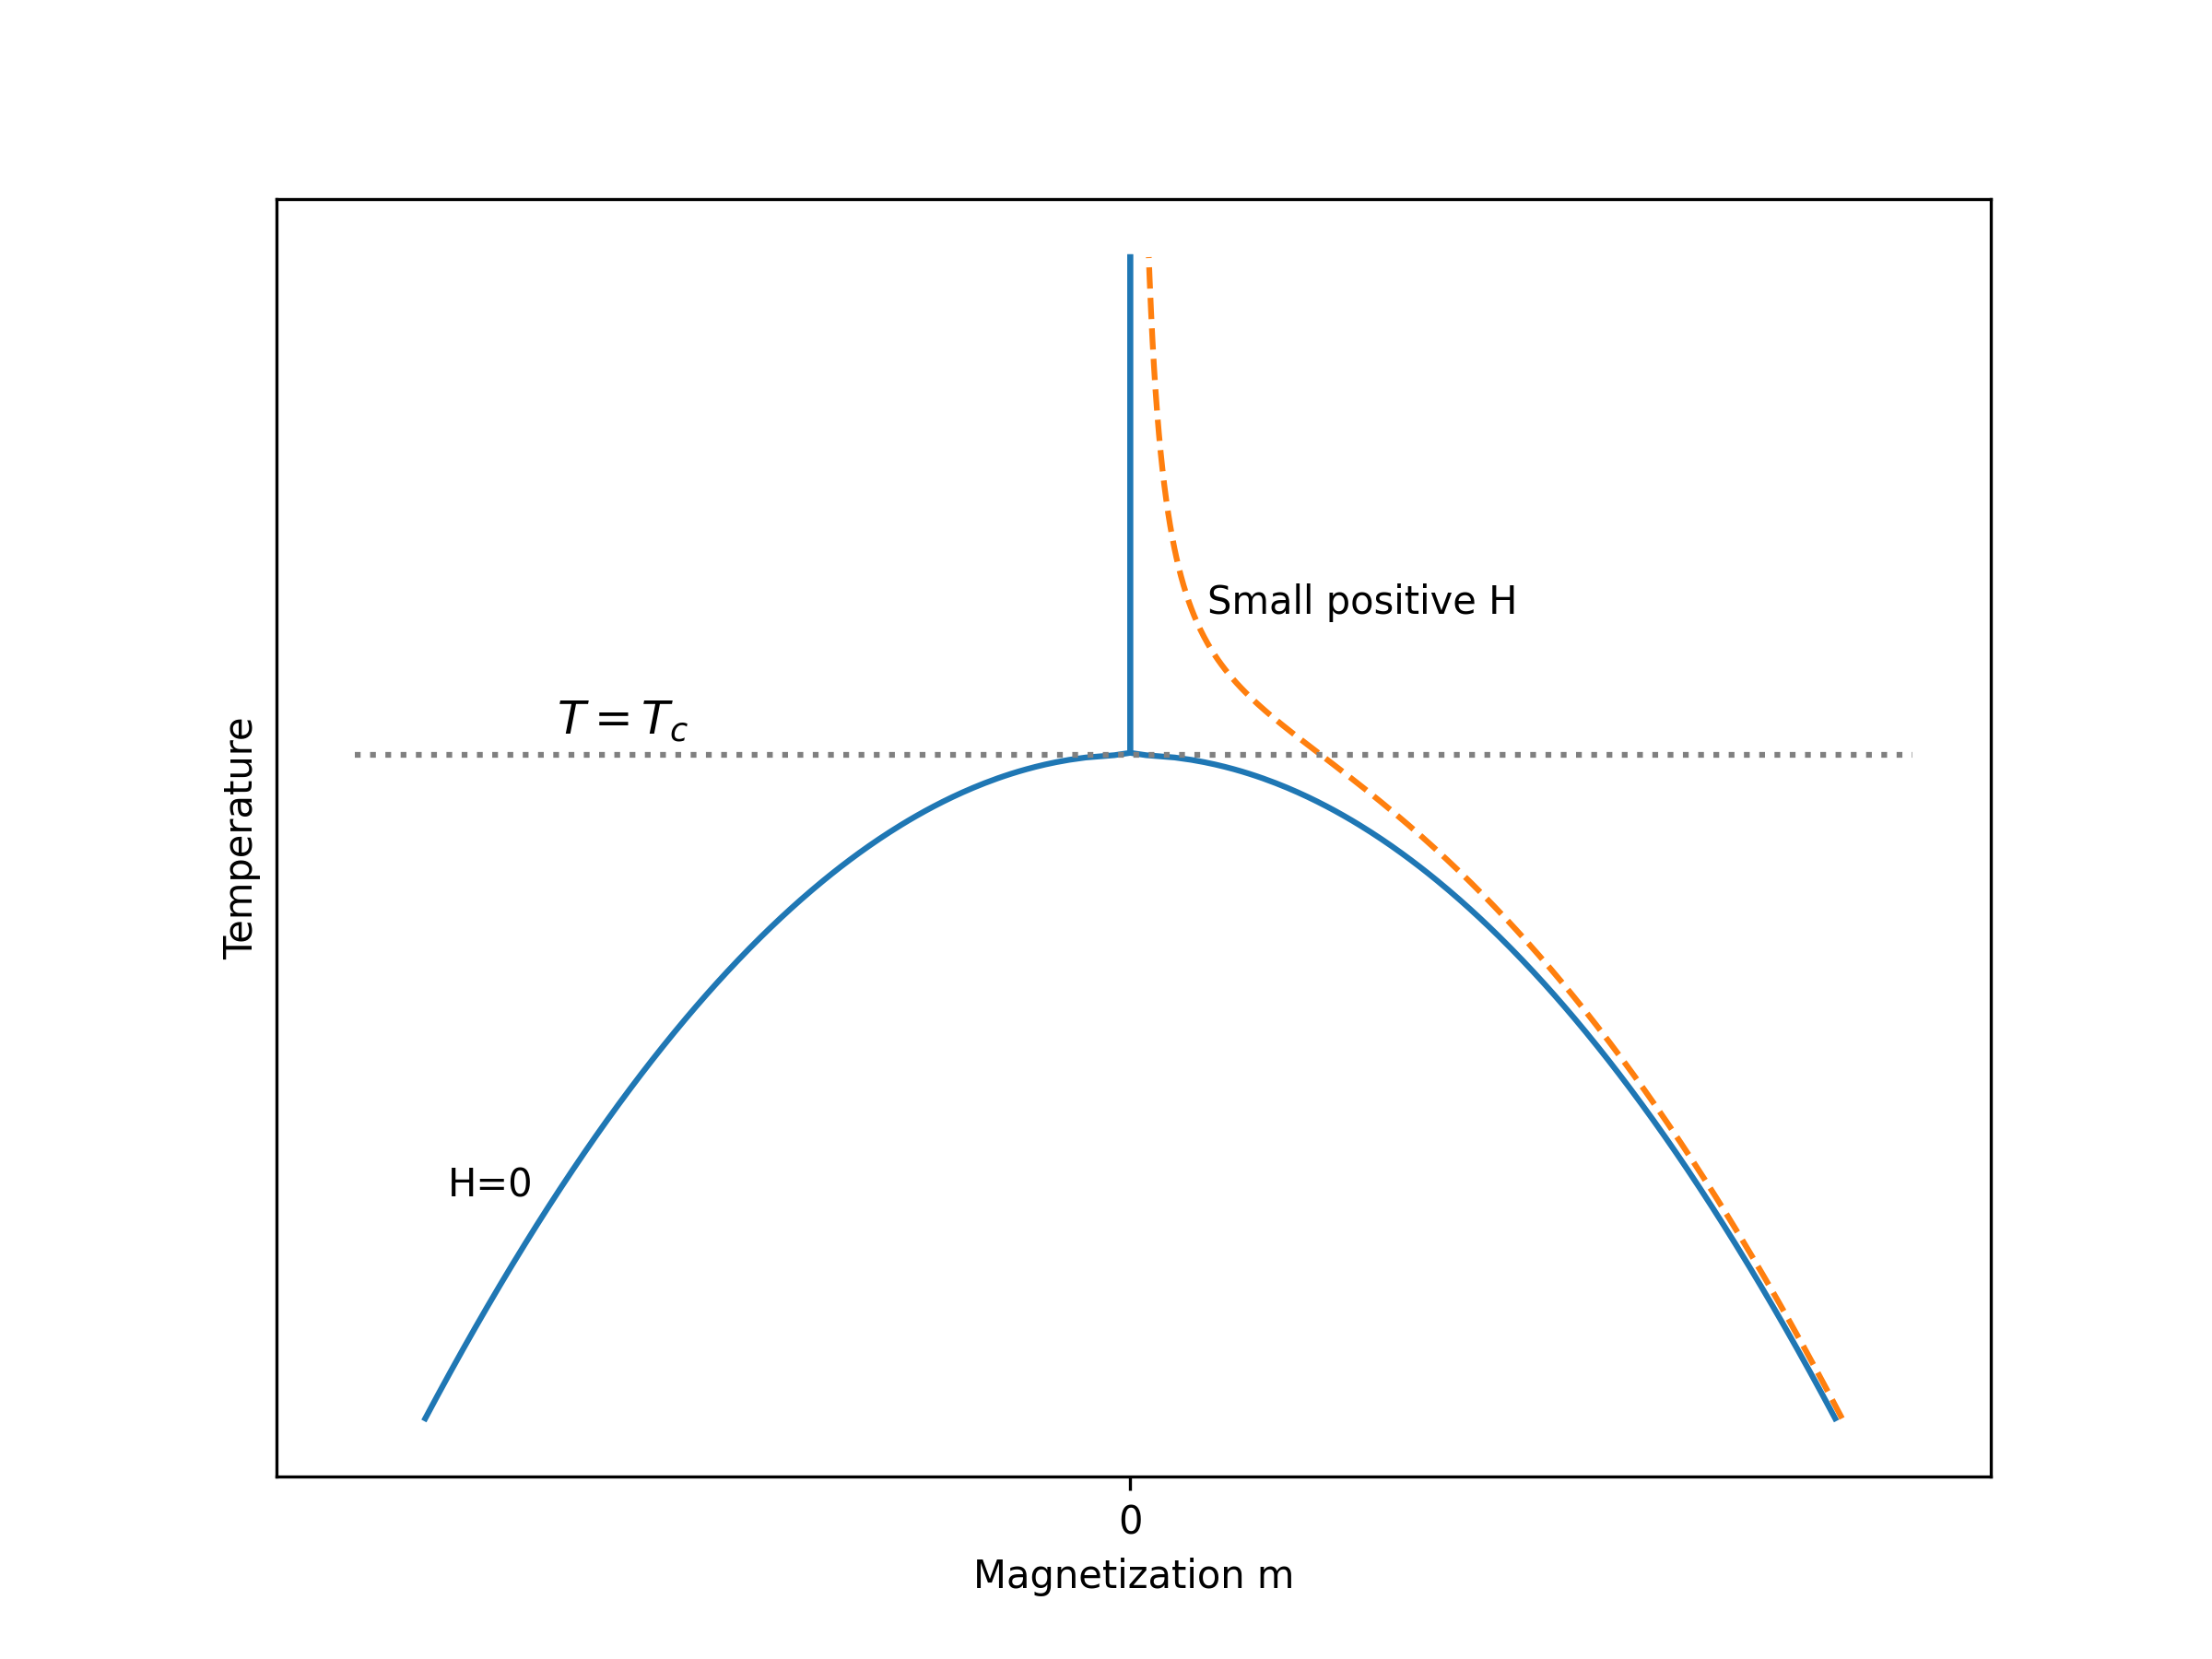
\includegraphics[width=0.7\linewidth,height=\textheight,keepaspectratio]{phase-transitions/Figs/isingmag_new.png}

}

\caption{\label{fig-isingmag}Phase diagram of a simple magnet in the
\(m\)-\(T\) plane.}

\end{figure}%

This shows the sudden change of behaviour at \(T_c\) (phase transition).
For \(T<T_c\) it is arbitrary which of the two roots \(\pm m^\star\) is
chosen; typically it will be different in different parts of the sample
(giving macroscopic ``magnetic domains''). But this behaviour with
temperature is \emph{qualitatively modified} by the presence of a field
\(H\), however small. In that case, there is always a slight
magnetization, even far above \(T_c\) and the curves becomes smoothed
out, as shown. There is no doubt which root will be chosen, and no
sudden change of the behaviour (no phase transition). Spontaneous
symmetry breaking does not occur, because the symmetry is already broken
by \(H\). (The curve \(F(m)\) is lopsided, rather than symmetrical about
\(m=0\).)

On the other hand, if we sit below \(T_c\) in a positive field (say) and
gradually reduce \(H\) through zero so that it becomes negative, there
is a \emph{very} sudden change of behaviour at \(h=0\): the equilibrium
state jumps discontinuously from \(m=m^\star\) to \(m=-m^\star\).

\begin{figure}

\centering{

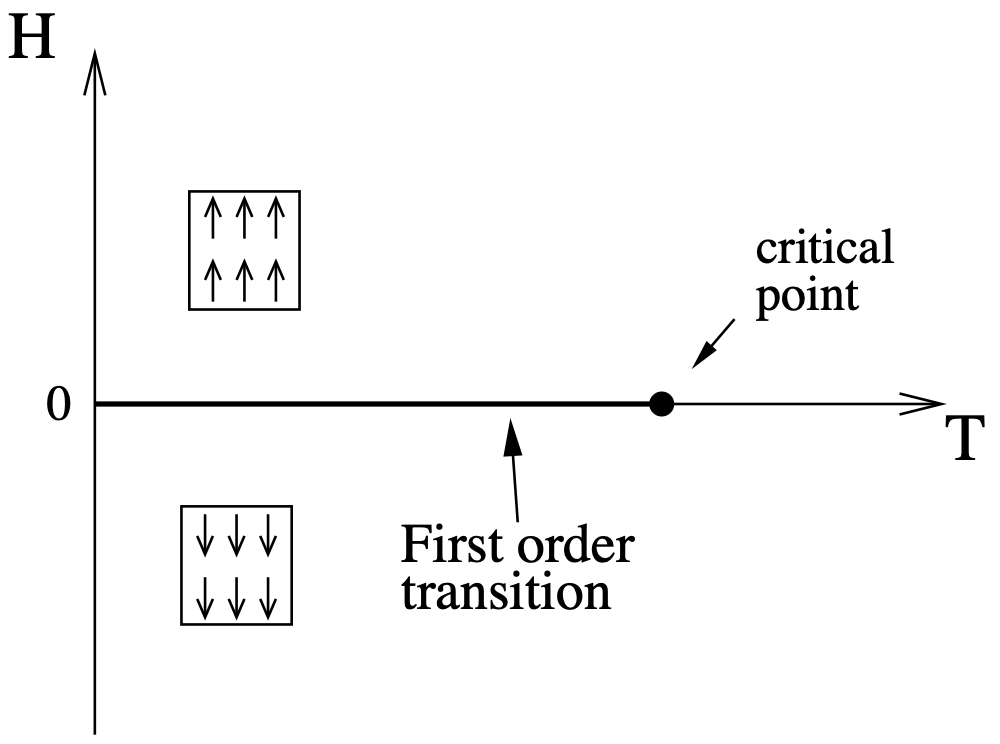
\includegraphics[width=0.7\linewidth,height=\textheight,keepaspectratio]{phase-transitions/Figs/isingpdH.png}

}

\caption{\label{fig-isingpdH}Phase diagram of a simple magnet in the
\(H\)-\(T\) plane.}

\end{figure}%

This is called a first order phase transition as opposed to the ``second
order'' or continuous transition that occurs at \(T_c\) in zero field.
The definitions are:

\emph{First order transition:} magnetisation (or similar order
parameter) depends discontinuously on a field variable (such as \(h\) or
\(T\)).

\emph{Continuous transition:} Change of functional form, but no
discontinuity in \(m\); typically, however,
\((\partial m/\partial T)_h\) (or similar) is either discontinuous, or
diverges with an integrable singularity.

In this terminology, we can say that the phase diagram of the magnet in
the \(H,T\) plane shows a line of first order phase transitions,
terminating at a continuous transition, which is the critical point.

\begin{tcolorbox}[enhanced jigsaw, toprule=.15mm, opacityback=0, colbacktitle=quarto-callout-caution-color!10!white, title=\textcolor{quarto-callout-caution-color}{\faFire}\hspace{0.5em}{Aside on Quantum Criticality}, leftrule=.75mm, rightrule=.15mm, bottomtitle=1mm, breakable, colframe=quarto-callout-caution-color-frame, colback=white, toptitle=1mm, left=2mm, titlerule=0mm, coltitle=black, arc=.35mm, bottomrule=.15mm, opacitybacktitle=0.6]

In some magnetic systems such as \(CePd_2Si_2\), one can, by applying
pressure or altering the chemical composition, depress the critical
temperature all the way to abolute zero! This may seem counterintuitive,
after all at \(T=0\) one should expect perfect ordering, not the large
fluctuations that accompany criticality. It turns out that the source of
the fluctuations that drive the system critical is zero point motion
associated with the Heisenberg uncertainty principle. Quantum
criticality is a matter of ongoing active research, and open questions
concern the nature of the phase diagrams and the relationship to
superconductivity. Although the subject goes beyond the scope of this
course, there is an accessible article
\href{https://arxiv.org/abs/1102.4628}{here} if you want to learn more.

\end{tcolorbox}

\section{A closer look: critical
exponents}\label{a-closer-look-critical-exponents}

Let us now see how we can calculate critical exponents within the mean
field approximation.

\subsection{Zero H solution and the order parameter
exponent}\label{zero-h-solution-and-the-order-parameter-exponent}

In zero field

\[m=\tanh(\frac{mT_c}{T})\] where \(T_c=qJ/k_B\) is the critical
temperature at which \(m\) first goes to zero.

We look for a solution where \(m\) is small (\(\ll 1\)). Expanding the
tanh function and replacing \(\beta=(k_BT)^{-1}\) yields

\[m=\frac{mT_c}{T}-\frac{1}{3}\left(\frac{mT_c}{T} \right)^3 +O(m^5)\:.\]
Then \(m=0\) is one solution. The other solution is given by

\[m^2=3\left(\frac{T}{T_c} \right)^3\left(\frac{T_c}{T} -1\right)\]

Now, considering temperatures close to \(T_c\) to guarantee small \(m\),
and employing the reduced temperature \(t=(T-T_c)/T_c\), one finds

\[m^2\simeq -3t\]

Hence

\begin{equation}\phantomsection\label{eq-mbeta}{\begin{aligned}
m= 0  &    ~~~\textrm{for } T>T_c \:\:\:  \textrm{ since~otherwise~{\it m}~imaginary}\nonumber\\
m= \pm\sqrt{-3t} & ~~\textrm{ for}  \:\:\: T<T_c ~~\textrm{ real}
\end{aligned} }\end{equation} This result implies that (within the mean
field approximation) the critical exponent \(\beta=1/2\).

\subsection{Finite (but small) field solution: the susceptibility
exponent}\label{sec:closerlook}

In a finite, but small field we can expand Equation~\ref{eq-mfmag} thus:

\[m=\frac{mT_c}{T}-\frac{1}{3}\left(\frac{mT_c}{T} \right)^3 +\frac{H}{kT}\]

Consider now the isothermal susceptibility

\[
\begin{aligned}
\chi  \equiv & \left(\frac{\partial m}{\partial H}\right)_T\\
      =     & \frac{T_c}{T}\chi - \left(\frac{T_c}{T}\right)^3 \chi m^2 + \frac{1}{k_BT}  
\end{aligned}
\]

Then

\[\chi \left[ 1-\frac{T_c}{T} +\left(\frac{T_c}{T}\right)^3m^2  \right]=\frac{1}{k_BT}\]

Hence near \(T_c\)

\[\chi=\frac{1}{k_BT_c}\left(\frac{1}{t+m^2}\right)\]

Then using the results of Equation~\ref{eq-mbeta}

\[
\begin{aligned}
\chi= (k_BT_ct)^{-1} & \textrm{ for} ~~~ T> T_c \\
\chi= (-2k_BT_ct)^{-1} & \textrm{ for}  ~~~T \le T_c 
\end{aligned} 
\]

where one has to take the non-zero value for \(m\) below \(T_c\) to
ensure +ve \(\chi\), i.e.~thermodynamic stability. This result implies
that (within the mean field approximation) the critical exponent
\(\gamma=1\).

The schematic behaviour of the Ising order parameter and susceptibility
are shown in Figure~\ref{fig-mfsum}~(a) and (b) respectively.

\begin{figure}

\begin{minipage}{0.50\linewidth}

\centering{

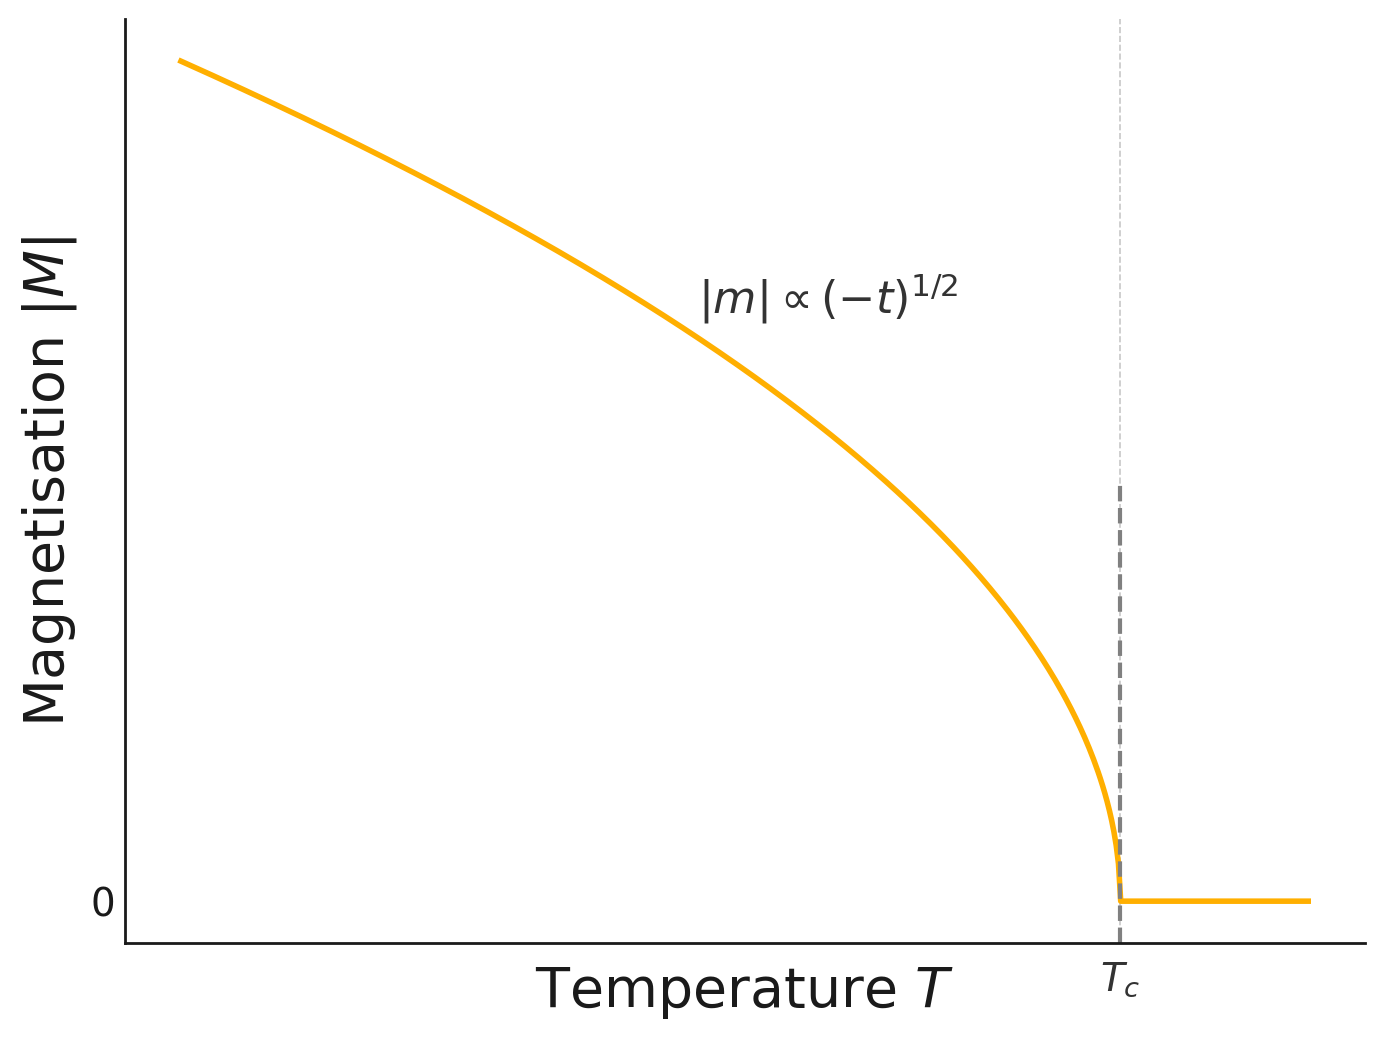
\includegraphics[width=1\linewidth,height=\textheight,keepaspectratio]{phase-transitions/Figs/mf_mag.png}

}

\subcaption{\label{fig-mfsum}Mean field behaviour of the Ising
magnetisation (schematic)}

\end{minipage}%
%
\begin{minipage}{0.50\linewidth}

\centering{

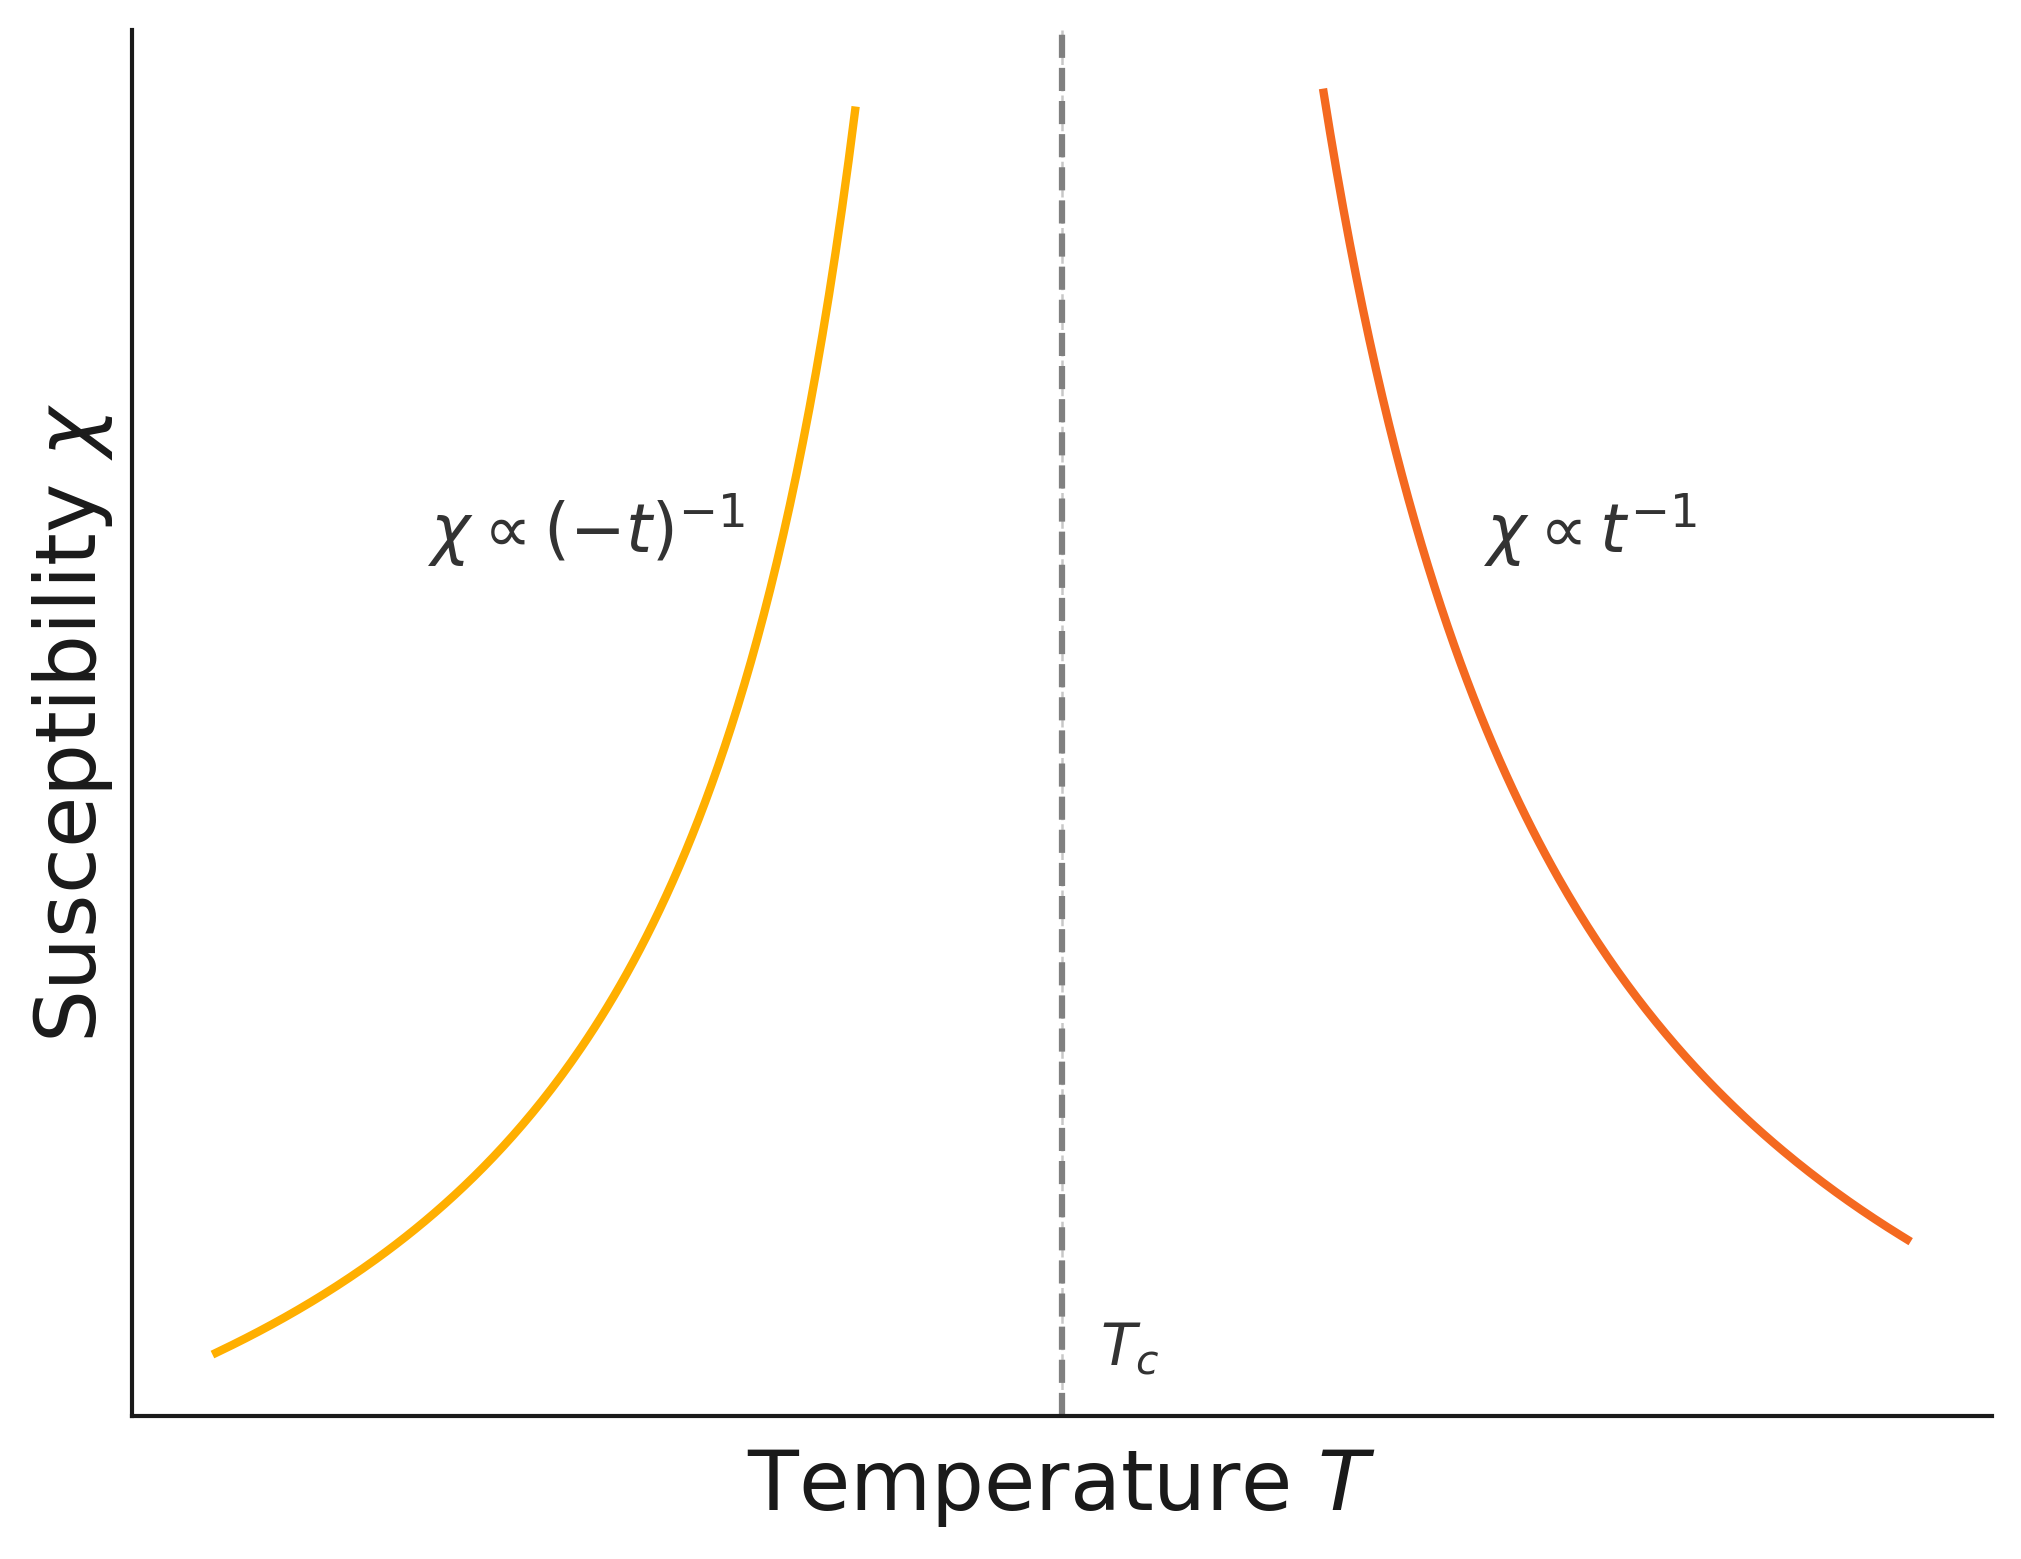
\includegraphics[width=1\linewidth,height=\textheight,keepaspectratio]{phase-transitions/Figs/mf_chi.png}

}

\subcaption{\label{fig-mfsum}Mean field behaviour of the Ising
susceptibility (schematic)}

\end{minipage}%

\end{figure}%

\section{Landau theory}\label{sec-landau-theory}

Landau theory is a slightly more general type of mean field theory than
that discussed in the previous subsection because it is not based on a
particular microscopic model. Its starting point is the Helmholtz free
energy, which Landau asserted can be written in terms of power series
expansion of the order parameter \(\phi\):

\[
F_(\phi)=\sum_{i=0}^{\infty}a_i\phi^i
\] The equilibrium value of \(\rho\) is that which minimises the Landau
free energy.

\begin{tcolorbox}[enhanced jigsaw, toprule=.15mm, opacityback=0, colbacktitle=quarto-callout-caution-color!10!white, title=\textcolor{quarto-callout-caution-color}{\faFire}\hspace{0.5em}{A note on order parameters}, leftrule=.75mm, rightrule=.15mm, bottomtitle=1mm, breakable, colframe=quarto-callout-caution-color-frame, colback=white, toptitle=1mm, left=2mm, titlerule=0mm, coltitle=black, arc=.35mm, bottomrule=.15mm, opacitybacktitle=0.6]

We have already seen examples of these in earlier sections, e.g., for
the liquid-gas transition this was \[
\rho_{liq} - \rho_{gas}: \quad \textrm{difference in density of two coexisting phases},
\] while for the Ising magnet it is the magnetisation \(m\). Both
quantities vanish at the critical point. These are examples of
\emph{scalar} order parameters -- a single number is required to
represent the degree of order (\(n = 1\)).

In the absence of a symmetry-breaking field, the Landau free-energy
density \(f_L\) must have symmetry \(f_L(-\phi) = f_L(\phi)\) (Ising
case).

For some other systems, \(n\) component vectors are required in order to
represent the order:

\[
\boldsymbol{\phi} = (\phi_1, \phi_2, \dots, \phi_n)
\]

Then \(f_L(\boldsymbol{\phi})\) should be symmetric under \(O(n)\)
rotations in \(n\)-component \(\phi\)-space.

The table below lists examples of order parameters for various physical
systems.

\begin{longtable}[]{@{}
  >{\raggedright\arraybackslash}p{(\linewidth - 4\tabcolsep) * \real{0.3478}}
  >{\raggedright\arraybackslash}p{(\linewidth - 4\tabcolsep) * \real{0.5130}}
  >{\raggedright\arraybackslash}p{(\linewidth - 4\tabcolsep) * \real{0.1391}}@{}}
\toprule\noalign{}
\begin{minipage}[b]{\linewidth}\raggedright
Physical System
\end{minipage} & \begin{minipage}[b]{\linewidth}\raggedright
Order Parameter \(\varphi\)
\end{minipage} & \begin{minipage}[b]{\linewidth}\raggedright
Symmetry Group
\end{minipage} \\
\midrule\noalign{}
\endhead
\bottomrule\noalign{}
\endlastfoot
Uniaxial (Ising) ferromagnet & Magnetisation per spin, \(m\) &
\(O(1)\) \\
Fluid (liquid-gas) & Density difference, \(\rho - \rho_c\) & \(O(1)\) \\
Liquid mixtures & Concentration difference, \(c - c_c\) & \(O(1)\) \\
Binary (AB) alloy (e.g., \(\beta\)-brass) & Concentration of one of the
species, \(c\) & \(O(1)\) \\
Isotropic (vector) ferromagnet & \(n\)-component magnetisation,
\(\mathbf{m} = (m_1, m_2, \dots, m_n)\) & \(O(n)\) \\
& \(n = 2\): \emph{xy} model & \(O(2)\) \\
& \(n = 3\): Heisenberg model & \(O(3)\) \\
Superfluid He\(^4\) & Macroscopic condensate wavefunction, \(\Psi\) &
\(O(2)\) \\
Superconductor (\emph{s}-wave) & Macroscopic condensate wavefunction,
\(\Psi\) & \(O(2)\) \\
Nematic liquid crystal & Orientational order,
\(\langle P_2(\cos \theta)\rangle\) & \\
Smectic A liquid crystal & 1-dimensional periodic density & \\
Crystal & 3-dimensional periodic density & \\
\end{longtable}

\textbf{Notes:}

\begin{itemize}
\tightlist
\item
  In \textbf{superfluid} \(^4He\) the order parameter is
\end{itemize}

\[
\Psi = |\Psi| e^{i\theta},
\]

the \emph{complex wavefunction} of the macroscopic condensate. Both the
amplitude \(|\Psi|\) and phase \(\theta\) must be specified, so this
corresponds to \(n = 2\).\\
\textbf{Superconductors} also correspond to \(n = 2\).

\begin{itemize}
\tightlist
\item
  In a \textbf{nematic} liquid crystal, the \emph{orientational} order
  parameter is
\end{itemize}

\[
\langle P_2(\cos \theta) \rangle \equiv \frac{1}{2}\langle 3\cos^2 \theta - 1\rangle,
\]

where \(\theta\) is the angle a molecule makes with the average
direction of the long axes of the molecules (known as the
\emph{director} \(\hat{n}\)). Rotational symmetry is broken. For the
case of an \(n\) component vector, the free energy should be a function
of:

\[
\phi^2 \equiv |\boldsymbol{\phi}|^2 = \phi_1^2 + \phi_2^2 + \dots + \phi_n^2 = \sum_{i=1}^n \phi_i^2
\] in the absence of a symmetry breaking field. Rotational symmetry is
incorporated into the theory.

\begin{figure}[H]

\begin{minipage}{0.50\linewidth}

\centering{

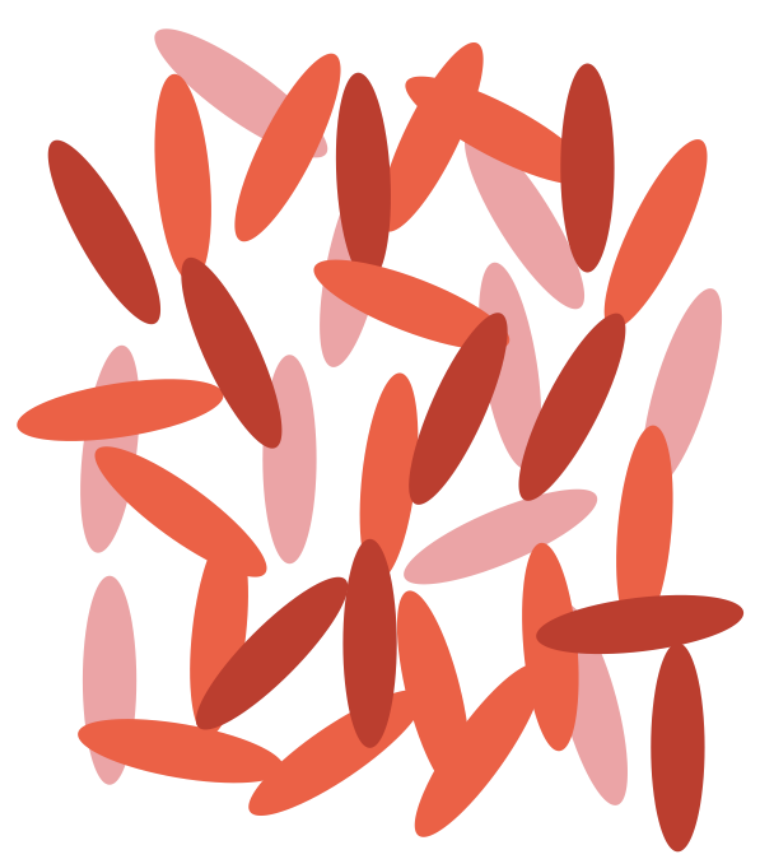
\includegraphics[width=0.5\linewidth,height=\textheight,keepaspectratio]{phase-transitions/Figs/isotropic-LC.png}

}

\subcaption{\label{fig-isotropic}Schematic of the isotropic liquid phase
of a system of elongated molcules.}

\end{minipage}%
%
\begin{minipage}{0.50\linewidth}

\centering{

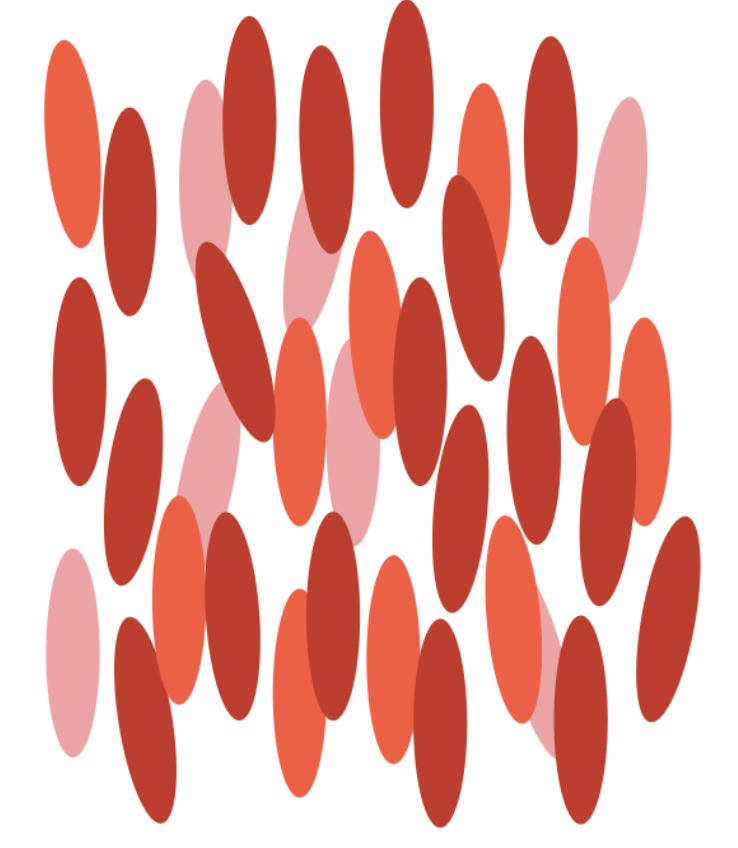
\includegraphics[width=0.5\linewidth,height=\textheight,keepaspectratio]{phase-transitions/Figs/nematic-LC.png}

}

\subcaption{\label{fig-isotropic}Schematic of the nematic liquid phase
of a system elongated molcules. This phase has uniaxial ordering.}

\end{minipage}%

\caption{\label{fig-mfsum}Isotropic and uniaxially ordered (nematic)
phases of liquid crystal molecules.}

\end{figure}%

\end{tcolorbox}

To exemplify the approach, let us specialise to the case of a
ferromagnet where \(\phi=m\), the magnetisation and write the Landau
free energy as

\begin{equation}\phantomsection\label{eq-landau}{
F(m)=F_0+a_2m^2+a_4m^4
}\end{equation}

Here only the terms compatible with the order parameter symmetry are
included in the expansion and we truncate the series at the 4th power
because this is all that is necessary to yield the essential
phenomenology. On symmetry grounds, the free energy of a ferromagnet
should be invariant under a reversal of the sign of the magnetisation.
Terms linear and cubic in \(m\) are not invariant under \(m\to -m\), and
so do not feature.

One can understand how the Landau free energy can give rise to a
critical point and coexistence values of the magnetisation, by plotting
\(F(m)\) for various values of \(a_2\) with \(a_4\) assumed positive
(which ensures that the magnetisation remains bounded). This is shown in
the following movie:

\url{Movies/landau_free_energy_evolution.mp4}

The situation is qualitatively similar to that discussed in
Section~\ref{sec-breaking}. Thermodynamics tells us that the system
adopts the state of lowest free energy. From the movie, we see that for
\(a_2>0\), the system will have \(m=0\), i.e.~will be in the disordered
(or paramagnetic) phase. For \(a_2<0\), the minimum in the free energy
occurs at a finite value of \(m\), indicating that the ordered
(ferromagnetic) phase is the stable one. In fact, the physical (up-down)
spin symmetry built into \(F\) indicates that there are two equivalent
stable states at \(m=\pm m^\star\). \(a_2=0\) corresponds to the
critical point which marks the border between the ordered and disordered
phases. Note that it is an inflexion point, so has
\(\frac{d^2F}{dm^2}=0\).

Clearly \(a_2\) controls the deviation from the critical temperature,
and accordingly we may write

\[a_2=\tilde{a_2} t\] where \(t\) is the reduced temperature. Thus we
see that the trajectory of the minima as a function of \(a_2<0\) in the
above movie effective traces out the coexistence curve in the \(m-T\)
plane.

We can now attempt to calculate critical exponents. Restricting
ourselves first to the magnetisation exponent \(\beta\) defined by
\(m=t^\beta\), we first find the equilibrium magnetisation,
corresponding to the minimum of the Landau free energy:

\begin{equation}\phantomsection\label{eq-minimize}{
\frac{dF}{dm}=2\tilde{a_2} tm+4a_4m^3=0
}\end{equation}

which implies

\[m\propto (-t)^{1/2},\] so \(\beta=1/2\), which is again a mean field
result.

Likewise we can calculate the effect of a small field \(H\) if we sit at
the critical temperature \(T_c\). Since \(a_2=0\), we have

\[F(m)=F_0+a_4m^4-Hm\]

\[\frac{\partial F}{\partial m}=0 \Rightarrow m(H,T_c)=\left(\frac{H}{4a_4}\right)^{1/3}\]

or

\[H \sim m^\delta ~~~~~ \delta=3\] which defines a second critical
exponent.

Note that at the critical point, a small applied field causes a very big
increase in magnetisation; formally, \((\partial m/\partial H)_T\) is
infinite at \(T=T_c\).

A third critical exponent can be defined from the magnetic
susceptibility at zero field

\[\chi=\left(\frac{\partial m}{\partial H}\right)_{T,V} \sim |T-T_c|^{-\gamma}\]

\emph{Exercise}: Show that the Landau expansion predicts \(\gamma=1\).

Finally we define a fourth critical exponent via the variation of the
heat capacity (per site or per unit volume) \(C_H\), in fixed external
field \(H=0\):

\[C_H \sim |T-T_c|^{-\alpha}\]

By convention, \(\alpha\) is defined to be positive for systems where
there is a \emph{divergence} of the heat capacity at the critical point
(very often the case). The heat capacity can be calculated from

\[C_H =-T\frac{\partial^2 F}{\partial T^2}\]

From the minimization over \(m\) @\#eq-minimize one finds
(\emph{exercise}: check this) \[
\begin{aligned}
F = & 0 ~~~~T>T_c\nonumber\\
F = & -a_2^2/4a_4 ~~~~ T < T_c
\end{aligned} 
\]

Using the fact that \(a_2\) varies linearly with \(T\), we have

\[
\begin{aligned}
C_H =& 0 ~~~~ T\to T_c^+\nonumber\\
C_H =& \frac{T\tilde a_2^2}{2a_4} ~~~~ T \to T_c^-\:,
\end{aligned} 
\]

which is actually a step discontinuity in specific heat. Since for
positive \(\alpha\) the heat capacity is divergent, and for negative
\(\alpha\) it is continuous, this behaviour formally corresponds to
\(\alpha=0\)

\section{Shortcomings of mean field
theory}\label{shortcomings-of-mean-field-theory}

While mean field theories provide a useful route to understanding
qualitatively the phenomenology of phase transitions, in real
ferromagnets, as well as in more sophisticated theories, the critical
exponents are not the simple fraction and integers found here. This
failure of mean field theory to predict the correct exponents is of
course traceable to their neglect of correlations. In later sections we
shall start to take the first steps to including the effects of long
range correlations.

\phantomsection\label{tab-exponents}
\begin{longtable}[]{@{}ccccc@{}}
\caption{Comparison of true Ising critical exponents with their mean
field theory predictions in a number of dimensions.}\tabularnewline
\toprule\noalign{}
\endfirsthead
\endhead
\bottomrule\noalign{}
\endlastfoot
\(\:\) & Mean Field & \(d=1\) & \(d=2\) & \(d=3\) \\
Critical temperature \(k_BT/qJ\) & \(1\) & \(0\) & \(0.5673\) &
\(0.754\) \\
Order parameter exponent \(\beta\) & \(\frac{1}{2}\) & - &
\(\frac{1}{8}\) & \(0.325 \pm 0.001\) \\
Susceptibility exponent \(\gamma\) & \(1\) & \(\infty\) &
\(\frac{7}{4}\) & \(1.24 \pm 0.001\) \\
Correlation length exponent \(\nu\) & \(\frac{1}{2}\) & \(\infty\) &
\(1\) & \(0.63\pm 0.001\) \\
\end{longtable}

\chapter{The Lattice Gas model}\label{the-lattice-gas-model}

A crude representation of a fluid is the lattice gas model. Here
particles can occupy the sites of a hypercubic lattice. The occupancy of
a site \(i\) is specified by the variable \(c_i=1\) (occupied) or
\(c_i=0\) vacant. The complete list of these occupancies \(\{c\}\)
specifies a microstate. The average particle number density (fraction of
occupied sites) is given by

\[c=L^{-d}\sum_i c_i \]

where \(L\) is the linear extent of the lattice and \(d\) its
dimensionality.

The Hamiltonian of the lattice gas model is

\[{\cal H}_{LG}=-\epsilon\sum_{<i,j>}c_ic_j - \mu\sum_ic_i\]

where \(\epsilon\) is an attraction energy between a pair of particles
on adjacent (nearest neighbouring) sites and \(\mu\) is a field known as
the chemical potential, which couples to the particle density which is
assumed to fluctuate around a mean value controlled by the prescribed
chemical potential. This representation of the model in which the
overall density fluctuates is known as the \emph{Grand Canonical
ensemble.}

\section{Mapping between Ising model and lattice
gas}\label{mapping-between-ising-model-and-lattice-gas}

The lattice gas model is interesting because whilst being a plausible
model for a fluid, it maps onto the Ising model. This extends the
applicability of the Ising model. To expose the mapping we write the
grand partition function of the lattice gas:

\[ \Xi=\sum_\textrm{ state}\exp-\beta{\cal H}_{LG}=\sum_{\{c\}}\exp\left[\beta \epsilon\sum_{<i,j>}c_ic_j +\beta\mu\sum_ic_i\right] \]
where the sum is an unrestricted sum over the occupancies of the lattice
sites. We now change variables to

\[c_i=(1+s_i)/2; ~~~~ J=\frac{\epsilon}{4} ~~~~
h=\frac{\epsilon q+2\mu}{4}\] Hence

\[{\cal H}_{LG}={\cal H}_\textrm{ I} + \textrm{ constant}\] Since the
last term does not depend on the configuration, it feeds through as an
additive constant in the free energy; and since all observables feature
as derivatives of the free energy, the constant has no physical
implications.

\section{Phase diagram}\label{phase-diagram-1}

Using these translation rules we can plot the phase diagram of the
lattice gas in the number density-temperature plane.

\begin{figure}

\centering{

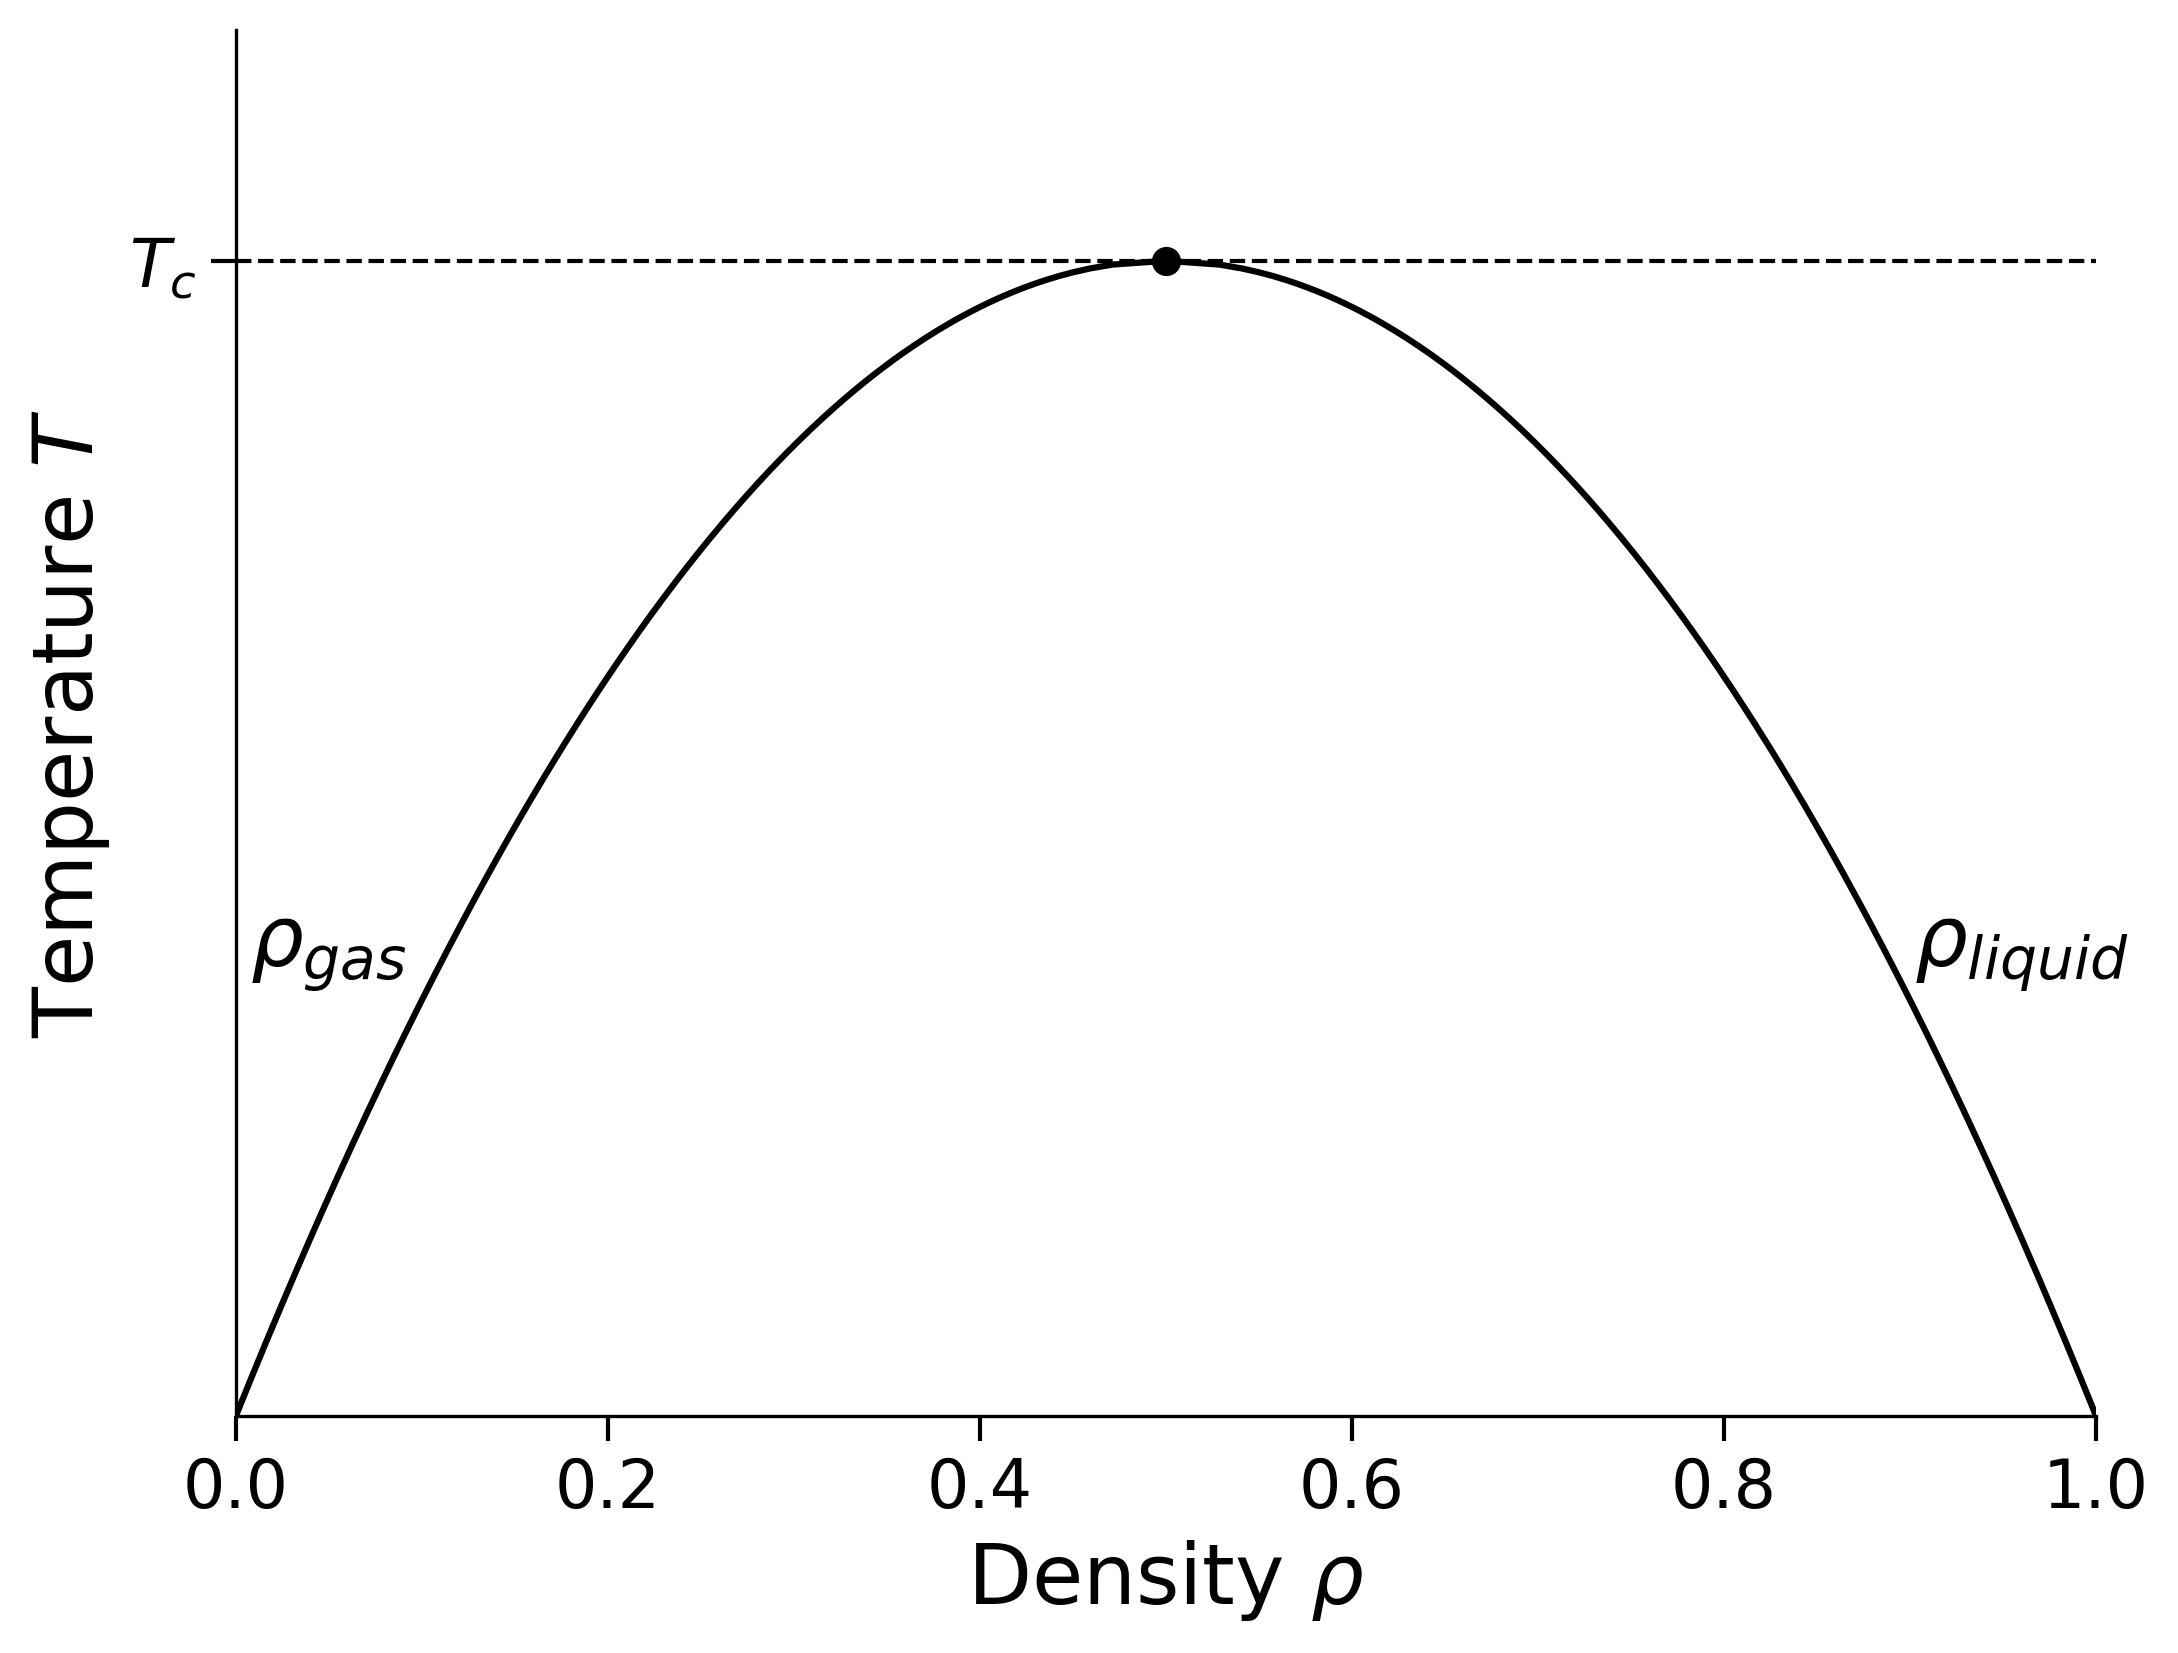
\includegraphics[width=0.6\linewidth,height=\textheight,keepaspectratio]{phase-transitions/Figs/lattice_gas_phase_diagram.png}

}

\caption{\label{fig-lattgas}Phase diagram of the lattice gas model in
the density-temperature plane.}

\end{figure}%

In the \(\mu-T\) plane there is a line of first order phase transitions
terminating at a critical point. The first order line means that if
\(T<T_c\) we smoothly increase the chemical potential through the
coexistence value of \(\mu\), the density of particles on our lattice
\(\rho=N/L^d\) jumps discontinuously from a low to a high value.

\[\rho_\textrm{ gas}=\frac{1-m^\star}{2} \to \rho_\textrm{ liquid}=\frac{1+m^\star}{2}
\] These values merge at \(T_c\), the gas-liquid critical point. At
higher temperatures, the distinction between the phases disappears.

\section{Real Fluids}\label{real-fluids}

You may wish to compare this with the results of (say) van der Waals
equation (see recommended textbooks for the required phase diagram). The
main difference is that the lattice gas has so-called ``particle-hole''
symmetry, \(\rho\to 1-\rho\) (inherited from the up-down symmetry of the
Ising model) which is not present for a real fluid. Accordingly, the
phase diagram in a real fluid looks like a lopsided version of the above
picture as shown in Figure~\ref{fig-realfluid}. See
\href{https://journals.aps.org/prl/pdf/10.1103/PhysRevLett.55.2160}{here}
for some real experimental data showing the asymmetry of the coexistence
curve in liquid metals.

\begin{figure}

\centering{

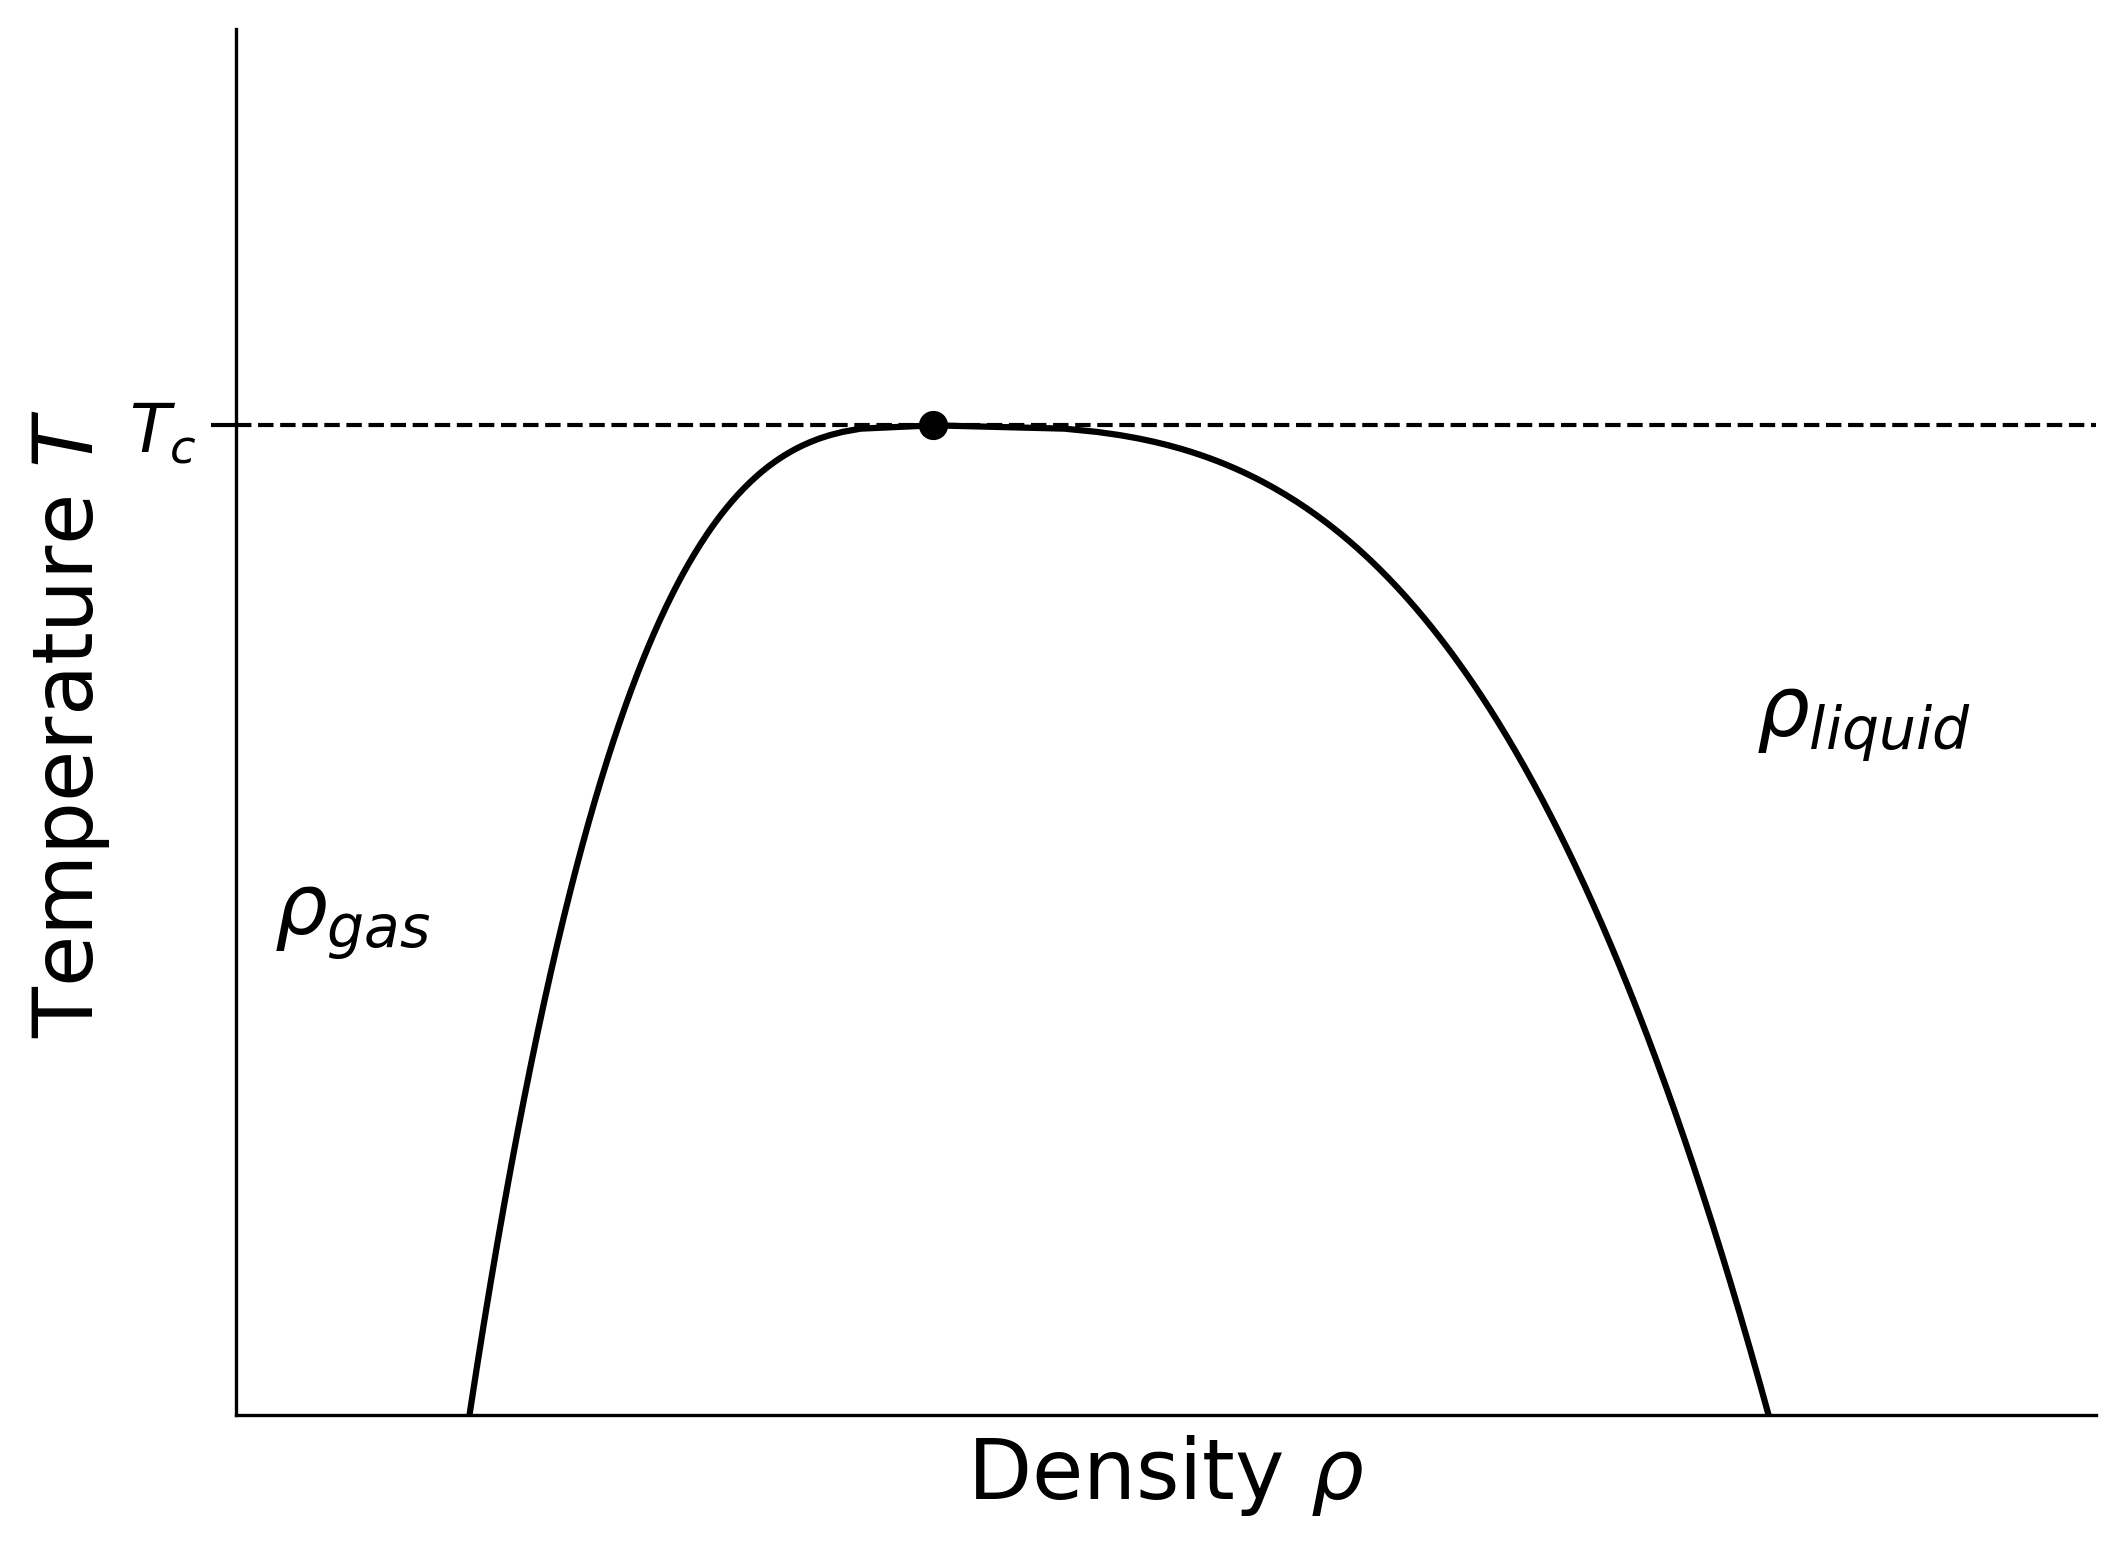
\includegraphics[width=0.6\linewidth,height=\textheight,keepaspectratio]{phase-transitions/Figs/real_fluid_pd_schem.png}

}

\caption{\label{fig-realfluid}Schematic of the liquid-gas phase diagram
in the \(\rho-T\) plane for a realistic fluid .}

\end{figure}%

\chapter{The Static Scaling
Hypothesis}\label{the-static-scaling-hypothesis}

Historically, the first step towards properly elucidating near-critical
behaviour was taken with the static scaling hypothesis. This is
essentially a plausible conjecture concerning the origin of power law
behaviour which appears to be consistent with observed phenomena.
According to the hypothesis, the basis for power law behaviour (and
associated scale invariance or ``scaling'') in near-critical systems is
expressed in the claim that: in the neighbourhood of a critical point,
the basic thermodynamic functions (most notably the free energy) are
\emph{generalized homogeneous functions} of their variables. For such
functions one can always deduce a scaling law such that by an
appropriate change of scale, the dependence on two variables (e.g.~the
temperature and applied field) can be reduced to dependence on one new
variable. This claim may be warranted by the following general argument.

A function of two variables \(g(u,v)\) is called a generalized
homogeneous function if it has the property

\[g(\lambda^au,\lambda^bv)=\lambda g(u,v)\] \textbf{for all
\(\lambda\)}, where the parameters \(a\) and \(b\) (known as scaling
parameters) are constants. An example of such a function is
\(g(u,v)=u^3+v^2\) with \(a=1/3, b=1/2\).

Now, the arbitrary scale factor \(\lambda\) can be redefined without
loss of generality as \(\lambda^a=u^{-1}\) giving

\[g(u,v)=u^{1/a}g(1,\frac{v}{u^{b/a}})\] A corresponding relation is
obtained by choosing the rescaling to be \(\lambda^b=v^{-1}\).

\[\label{eq:sca2}
g(u,v)=v^{1/b}g(\frac{u}{v^{a/b}},1)\]

This equation demonstrates that \(g(u,v)\) indeed satisfies a simple
power law in \(\it{one}\) variable, subject to the constraint that
\(u/v^{a/b}\) is a constant. It should be stressed, however, that such a
scaling relation specifies neither the function \(g\) nor the parameters
\(a\) and \(b\).

Now, the static scaling hypothesis asserts that in the critical region,
the free energy \(F\) is a generalized homogeneous function of the
(reduced) thermodynamic fields \(t=(T-T_c)/T_c\) and \(h=(H-H_c)\).
Remaining with the example ferromagnet, the following scaling assumption
can then be made:

\[F(\lambda^a t,\lambda^b h)=\lambda F(t,h) \:.
\label{eq:scagibbs}\]

Without loss of generality, we can set \(\lambda^a=t^{-1}\), implying
\(\lambda=t^{-1/a}\) and \(\lambda^b=t^{-b/a}\).

Then \[F(t,h)=t^{1/a}F(1,t^{-b/a}h)\] where our choice of \(\lambda\)
ensures that \(F\) on the rhs is now a function of a single variable
\(t^{-b/a}h\).

Now, as stated in Chapter~\ref{sec-background}, the free energy provides
the route to all thermodynamic functions of interest. An expression for
the magnetisation can be obtained simply by taking the field derivative
of \(F\) (cf. Figure~\ref{fig-thermo})

\begin{equation}\phantomsection\label{eq-magscale}{m(t,h)=-t^{(1-b)/a}m(1,t^{-b/a}h)
}\end{equation}

In zero applied field \(h=0\), this reduces to

\[m(t,0)=(-t)^{(1-b)/a}m(1,0)\] where the r.h.s. is a power law in
\(t\). Equation~\ref{eq-mag} then allows identification of the exponent
\(\beta\) in terms of the scaling parameters \(a\) and \(b\).

\[\beta=\frac{1-b}{a}\]

By taking further appropriate derivatives of the free energy, other
relations between scaling parameters and critical exponents may be
deduced. Such calculations (\emph{Exercise: try to derive them}) yield
the results \(\delta =
b/(1-b)\),\(\gamma = (2b-1)/a\), and \(\alpha =(2a-1)/a\) .
Relationships between the critical exponents themselves can be obtained
trivially by eliminating the scaling parameters from these equations.
The principal results (known as ``scaling laws'') are:- \[
\begin{aligned}
\alpha+\beta(\delta+1)=2 \\
\alpha+2\beta+\gamma=2
\end{aligned} 
\]

Thus, provided all critical exponents can be expressed in terms of the
scaling parameters \(a\) and \(b\), then only two critical exponents
need be specified, for all others to be deduced. Of course these scaling
laws are also expected to hold for the appropriate thermodynamic
functions of analogous systems such as the liquid-gas critical point.

\section{Experimental Verification of
Scaling}\label{experimental-verification-of-scaling}

The validity of the scaling hypothesis finds startling verification in
experiment. To facilitate contact with experimental data for real
systems, consider again Equation~\ref{eq-magscale}. Eliminating the
scaling parameters \(a\) and \(b\) in favour of the exponents \(\beta\)
and \(\delta\) gives

\[
\frac{m(t,h)}{t^{\beta}}=m(1,\frac{h}{t^{\beta\delta}})
\] where the RHS of this last equation can be regarded as a function of
the single scaled variable \(\tilde{H} \equiv t^{-\beta\delta} h(t,M)\).

For some particular magnetic system, one can perform an experiment in
which one measures \(m\) vs \(h\) for various fixed temperatures. This
allows one to draw a set of isotherms, i.e.~\(m-h\) curves of constant
\(t\). These can be used to demonstrate scaling by plotting the data
against the scaling variables \(M=t^{-\beta}m(t,h)\) and
\(\tilde{H}=t^{-\beta\delta}h(t,M)\). Under this scale transformation,
it is found that all isotherms (for \(t\) close to zero) coincide to
within experimental error. Reassuringly, similar results are found using
the scaled equation of state of simple fluid systems such as He\(^3\) or
Xe.

\begin{figure}

\centering{

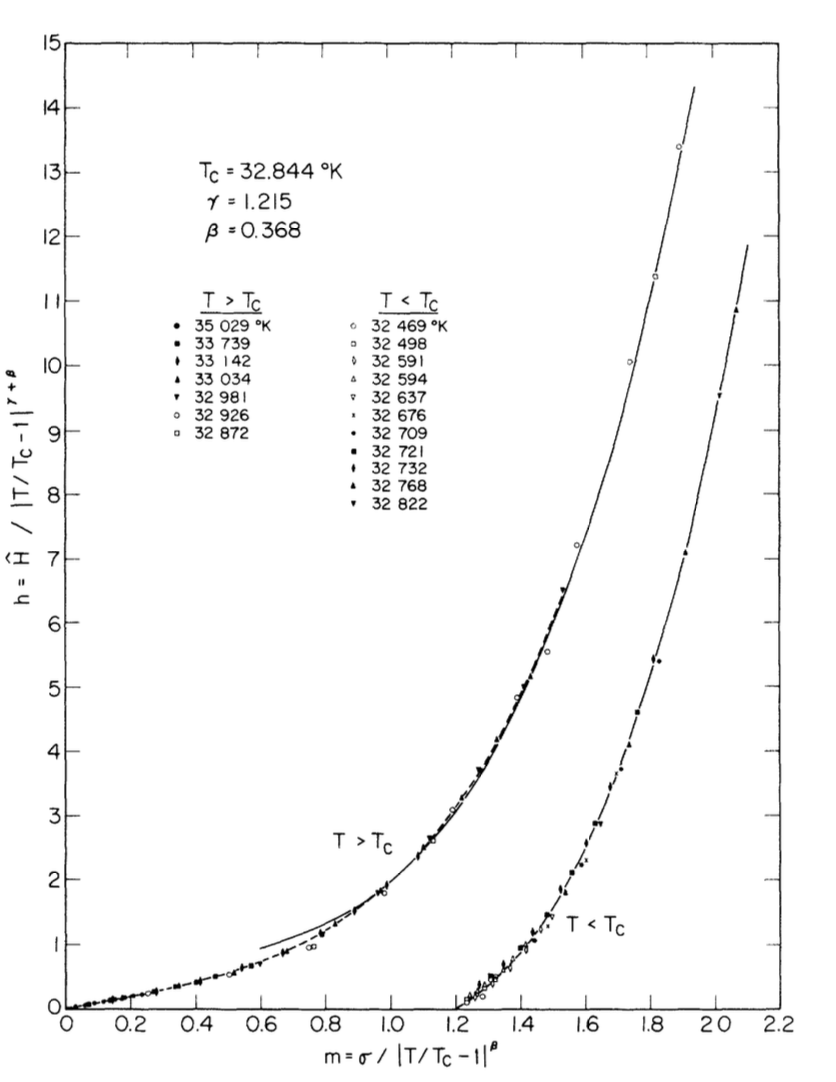
\includegraphics[width=0.7\linewidth,height=\textheight,keepaspectratio]{phase-transitions/Figs/scaling.png}

}

\caption{\label{fig-scalingexp}Magnetisation of CrBr\(_3\) in the
critical region plotted in scaled form (see text). From
\href{https://journals.aps.org/prl/abstract/10.1103/PhysRevLett.22.603}{Ho
and Lister (1969)}.}

\end{figure}%

In summary, the static scaling hypothesis is remarkably successful in
providing a foundation for the observation of power laws and scaling
phenomena. However, it furnishes little or no guidance regarding the
role of co-operative phenomena at the critical point. In particular it
provides no means for calculating the values of the critical exponents
appropriate to given model systems.

\section{Computer simulation}\label{sec-compsim}

In seeking to employ simulation to obtain estimates of bulk critical
point properties (such as the location of a critical point and the
values of its associated exponents), one is immediately confronted with
a difficulty. The problem is that simulations are necessarily restricted
to dealing with systems of finite-size and cannot therefore accommodate
the truly long ranged fluctuations that characterize the near-critical
regime. As a consequence, the critical singularities in \(C_v\), order
parameter, etc. appear rounded and shifted in a simulation study.
Figure~\ref{fig-shift} shows a schematic example for the susceptibility
of a magnet.

\begin{figure}

\centering{

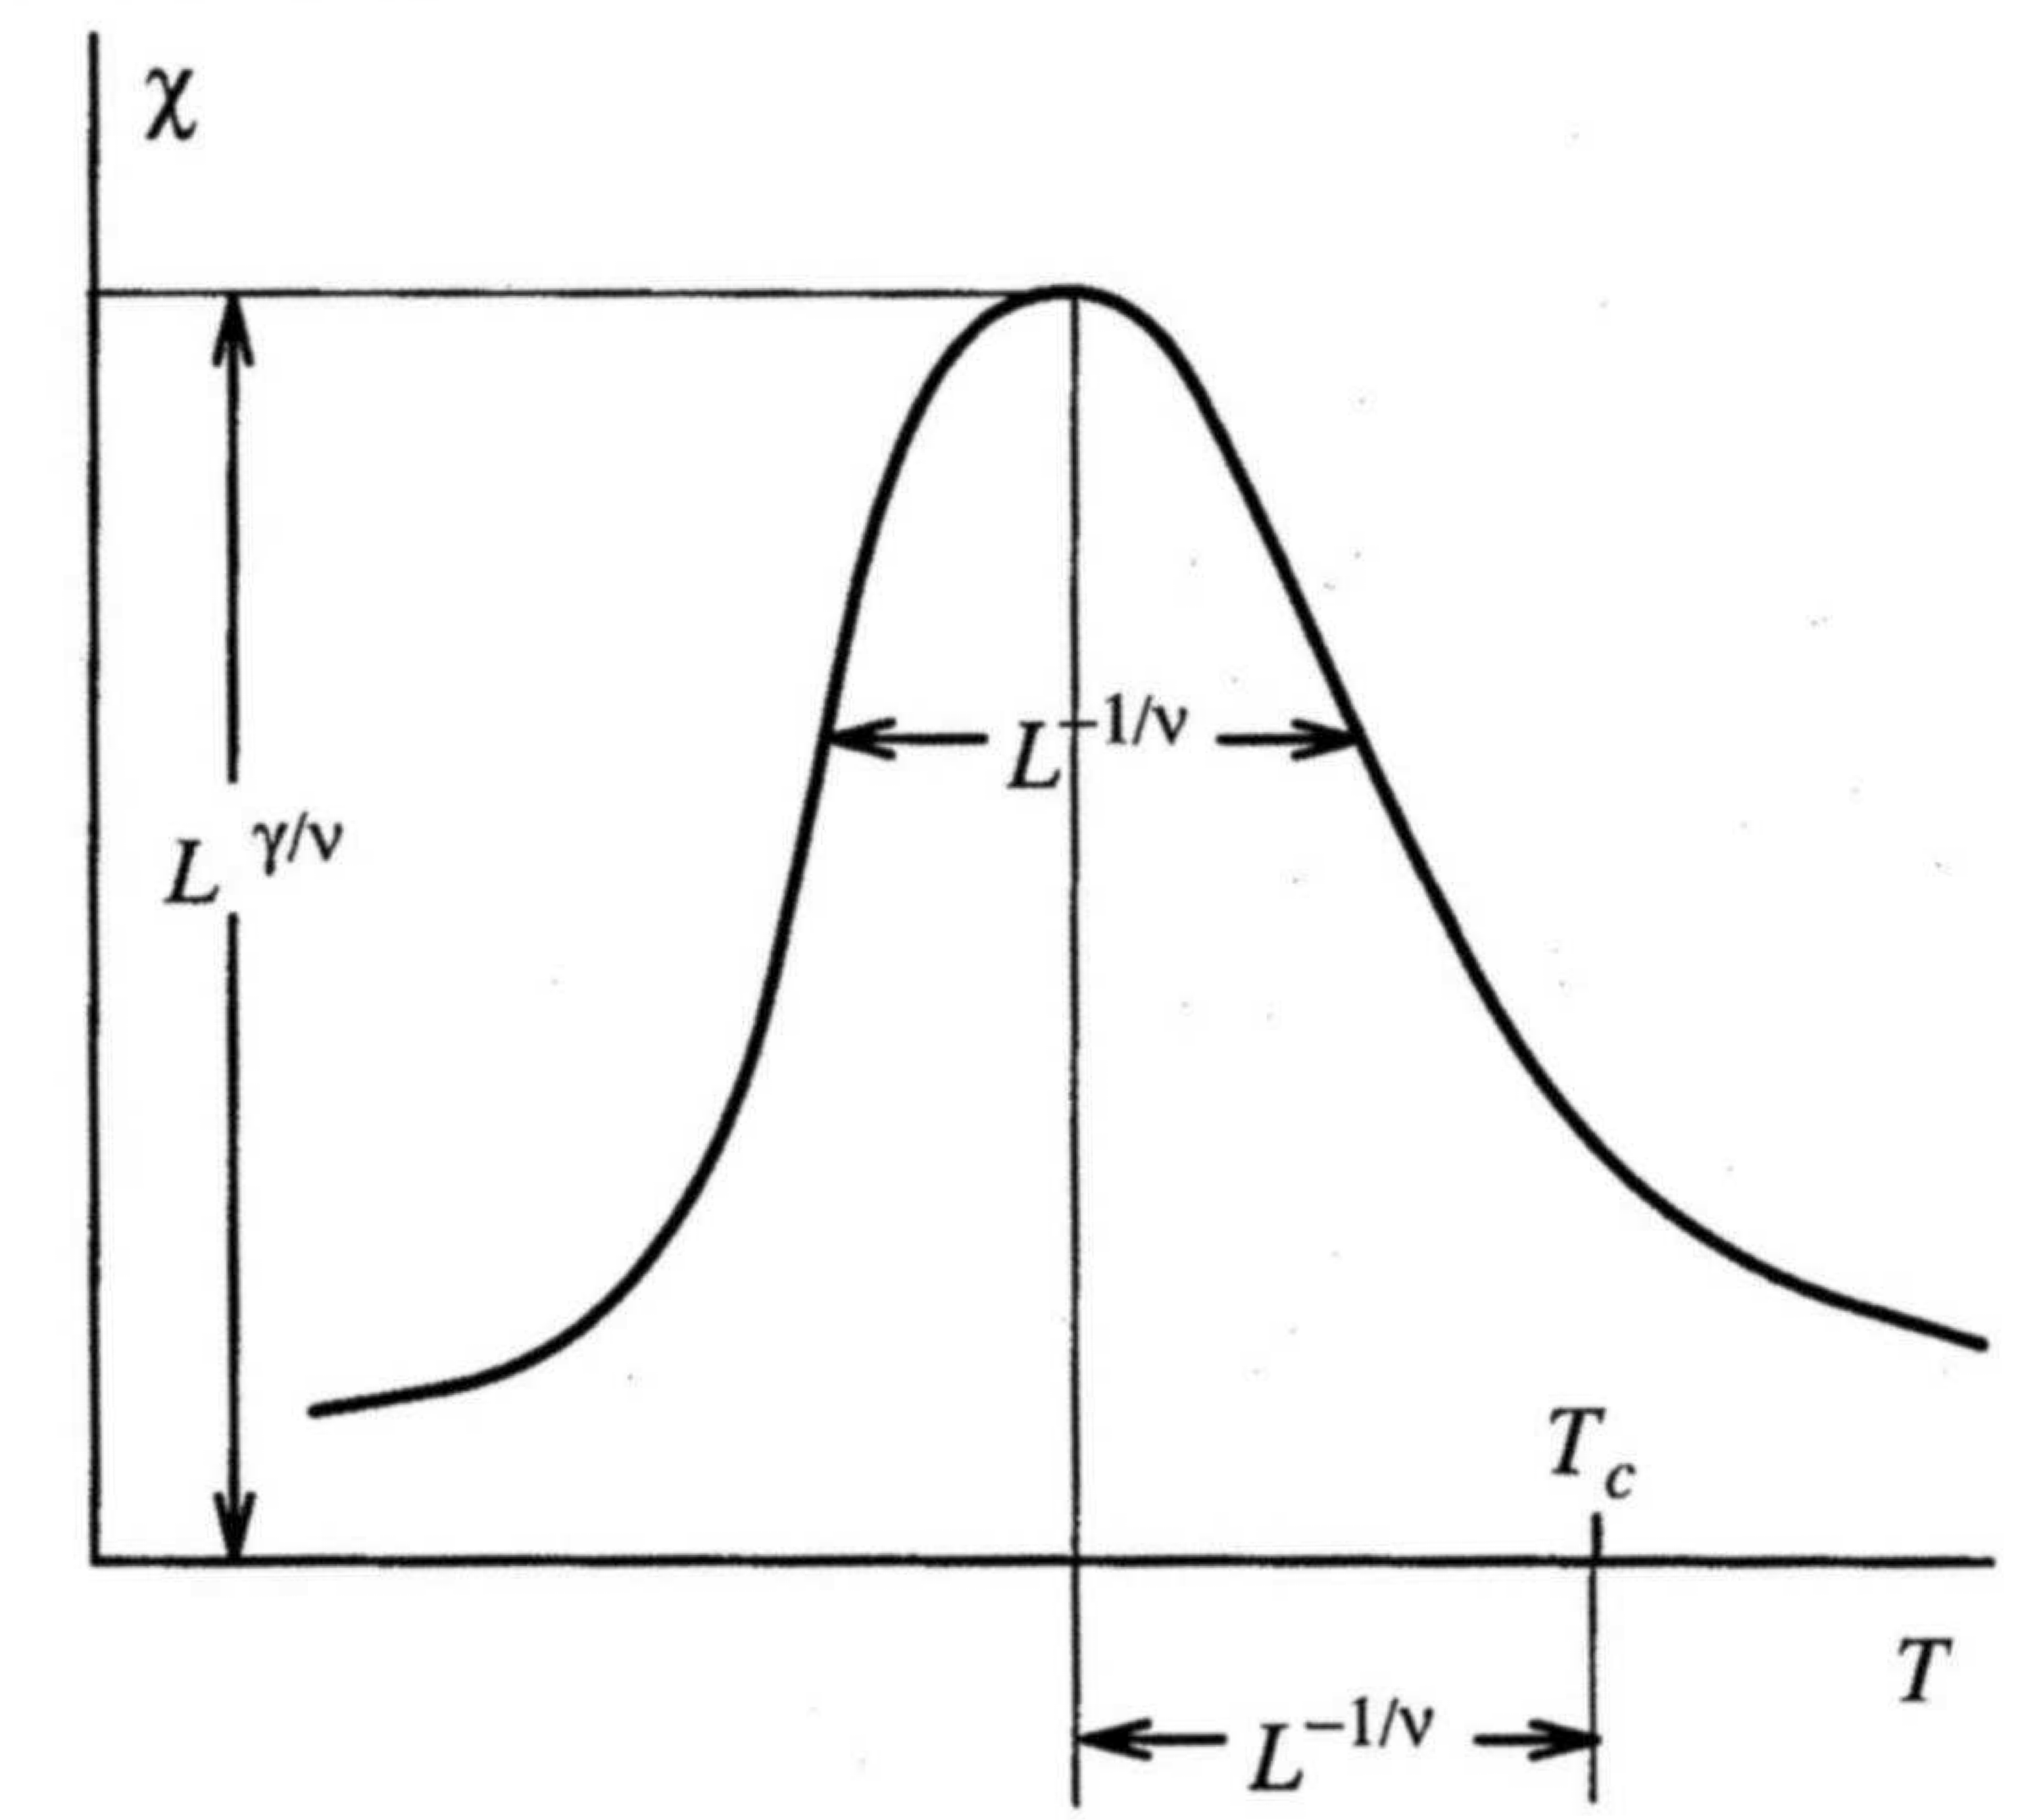
\includegraphics[width=0.6\linewidth,height=\textheight,keepaspectratio]{phase-transitions/Figs/shift.png}

}

\caption{\label{fig-shift}Schematic of the near-critical temperature
dependence of the magnet susceptibility in a finite-sized system.}

\end{figure}%

Thus the position of the peak in a response function (such as \(C_v\))
measured for a finite-sized system does not provide an accurate estimate
of the critical temperature. Although the degree of rounding and
shifting reduces with system size, it is often the case, that
computational constraints prevent access to the largest system sizes
which would provide accurate estimates of critical parameters. To help
deal with this difficulty, finite-size scaling (FSS) methods have been
developed to allow extraction of bulk critical properties from
simulations of finite size. FSS will be discussed in
Section~\ref{sec-fss}

\chapter{Universality and the Renormalisation Group Theory of Critical
Phenomena}\label{universality-and-the-renormalisation-group-theory-of-critical-phenomena}

\emph{Owing the the absence of a wholly appropriate textbook for the
material covered in this section, I have supplied more detailed notes
than used in other parts of the unit.}

The critical region is characterised by correlated microstructure on
\(\underline{all}\) length-scales up to and including the correlation
length. Such a profusion of degrees of freedom can only be accurately
characterized by a very large number of variables. Mean field theories
and approximation schemes fail in the critical region because they at
best incorporate interactions among only a few spins, while neglecting
correlations over larger distances. Similarly, the scaling hypothesis
fails to provide more than a qualitative insight into the nature of
criticality because it focuses on only one length-scale, namely the
correlation length itself. Evidently a fuller understanding of the
critical region may only be attained by taking account of the existence
of structure on all length-scales. Such a scheme is provided by the
renormalisation group method, which stands today as the cornerstone of
the modern theory of critical phenomena.

\section{The critical point: A many length scale
problem}\label{the-critical-point-a-many-length-scale-problem}

A near critical system can be characterized by three important length
scales, namely

\begin{enumerate}
\def\labelenumi{\arabic{enumi}.}
\item
  The correlation length, \(\xi\), ie the size of correlated
  microstructure.
\item
  Minimum length scale \(L_\textrm{ min}\), i.e.~the smallest length in
  the microscopics of the problem, e.g.~lattice spacing of a magnet or
  the particle size in a fluid.
\item
  Macroscopic size \(L_{max}\) eg. size of the system.
\end{enumerate}

The authentic critical region is defined by a window condition:

\[L_\textrm{ max} \gg \xi \gg L_\textrm{ min}\]

The physics of this regime is hard to tackle by analytic theory because
it is characterized by configurational structure on all scales between
\(L_\textrm{ min}\) and \(\xi\) (in fact it turns out that the near
critical configurational patterns are \emph{fractal}-like, cf.
Figure~\ref{fig-ssb}. Moreover different length scales are correlated
with one another, giving rise to a profusion of coupled variables in any
theoretical description. The window regime is also not easily accessed
by computer simulation because it entails studying very large system
sizes \(L_\textrm{
max}\), often requiring considerable computing resources.

\section{Methodology of the RG}\label{sec-rgmethod}

The central idea of the renormalisation group (RG) method is a stepwise
elimination of the degrees of freedom of the system on successively
larger length-scales. To achieve this one introduces a fourth length
scale \(L\). In contrast to the other three, which characterize the
system itself, \(L\) characterises the \emph{description} of the system.
It may be thought of as typifying the size of the smallest resolvable
detail in a description of the system's microstructure.

Consider the Ising model arrangements displayed in
Figure~\ref{fig-snapshots}. These pictures contain \emph{all} the
details of each configuration shown: the resolution length \(L\) in this
case has its smallest possible value, coinciding with the lattice
spacing i.e.~\(L=L_{\min}\). In the present context, the most detailed
description is not the most useful: the essential signals with which we
are concerned are hidden in a noise of relevant detail. A clue to
eliminating this noise lies in the nature of the correlation length,
i.e.~the size of the largest droplets. The explicit form of the small
scale microstructure is irrelevant to the behaviour of \(\xi\). The
small scale microstructure is the noise. To eliminate it, we simply
select a larger value of the resolution length (or `coarse-graining'
length) \(L\).

There are many ways of implementing this coarse-graining procedure. We
adopt a simple strategy in which we divide our sample into blocks of
side \(L\), each of which contains \(L^d\) sites, with \(d\) the space
dimensions . The centres of the blocks define a lattice of points
indexed by \(I=1,2,N/L^d\). We associate with each block lattice point
centre, \(I\), a coarse-grained or block variable \(S_I(L)\) defined as
the spatial average of the local variables it contains:

\begin{equation}\phantomsection\label{eq-blkvar}{
S_I(L)=L^{-d}\sum_i^Is_i
}\end{equation} where the sum extends over the \(L^d\) sites in the
block \(I\). The set of coarse grained coordinates \(\{S(L)\}\) are the
basic ingredients of a picture of the system having spatial resolution
of order \(L\).

The coarse graining operation is easily implemented on a computer. In so
doing one is faced with the fact that while the underlying Ising spins
can only take two possible values, the block variables \(S_I(L)\) have
\(L^d+1\) possible values. Accordingly in displaying the consequences of
the blocking procedure, we need a more elaborate colour convention than
that used in Figure~\ref{fig-snapshots}. We will associate with each
block a shade of grey drawn from a spectrum ranging from black to white.

\begin{figure}

\begin{minipage}{0.50\linewidth}

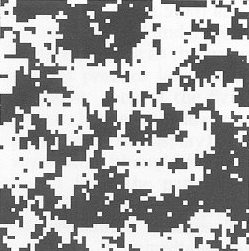
\includegraphics[width=0.5\linewidth,height=\textheight,keepaspectratio]{phase-transitions/Figs/a1_2state.png}

\subcaption{\label{}(ai)}
\end{minipage}%
%
\begin{minipage}{0.50\linewidth}

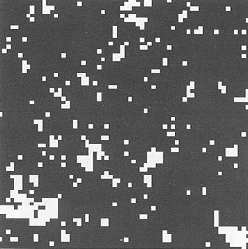
\includegraphics[width=0.5\linewidth,height=\textheight,keepaspectratio]{phase-transitions/Figs/b1_2state.png}

\subcaption{\label{}(bi)}
\end{minipage}%
\newline
\begin{minipage}{0.50\linewidth}

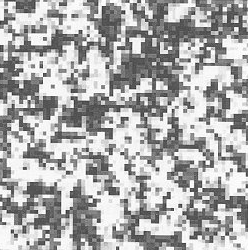
\includegraphics[width=0.5\linewidth,height=\textheight,keepaspectratio]{phase-transitions/Figs/a2_2state.png}

\subcaption{\label{}(aii)}
\end{minipage}%
%
\begin{minipage}{0.50\linewidth}

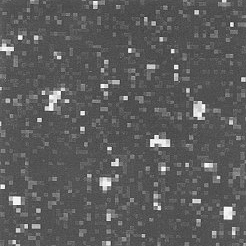
\includegraphics[width=0.5\linewidth,height=\textheight,keepaspectratio]{phase-transitions/Figs/b2_2state.png}

\subcaption{\label{}(bii)}
\end{minipage}%
\newline
\begin{minipage}{0.50\linewidth}

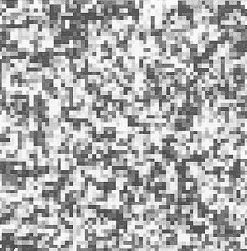
\includegraphics[width=0.5\linewidth,height=\textheight,keepaspectratio]{phase-transitions/Figs/a3_2state.png}

\subcaption{\label{}(aiii)}
\end{minipage}%
%
\begin{minipage}{0.50\linewidth}

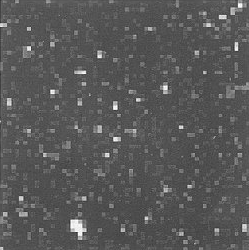
\includegraphics[width=0.5\linewidth,height=\textheight,keepaspectratio]{phase-transitions/Figs/b3_2state.png}

\subcaption{\label{}(biii)}
\end{minipage}%
\newline
\begin{minipage}{0.50\linewidth}

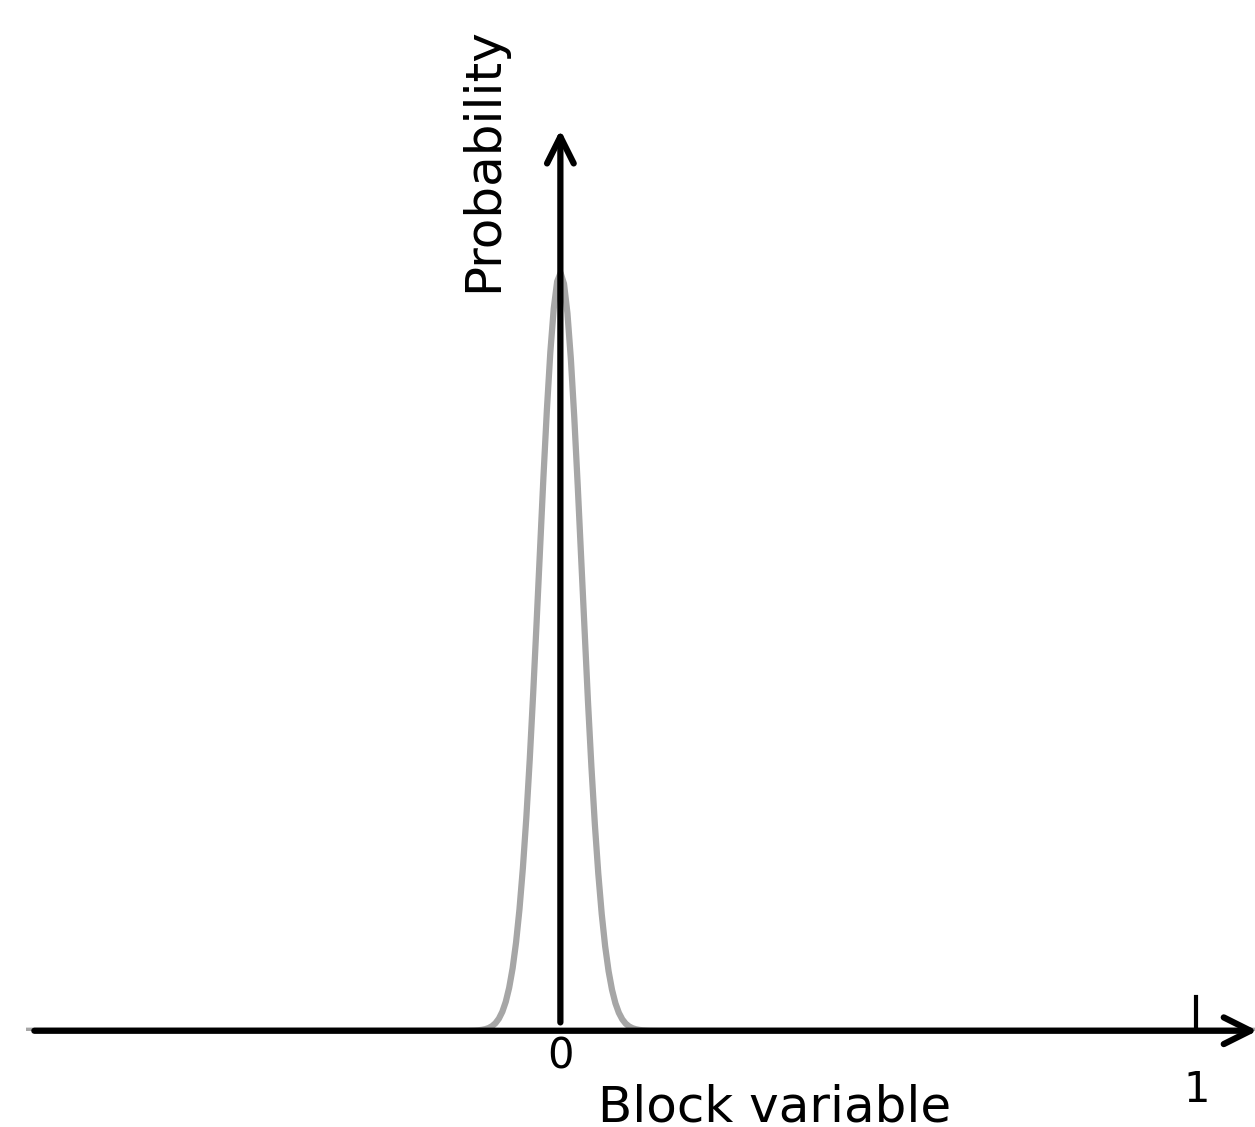
\includegraphics[width=0.6\linewidth,height=\textheight,keepaspectratio]{phase-transitions/Figs/schem_op_disordered.png}

\subcaption{\label{}(aiv)}
\end{minipage}%
%
\begin{minipage}{0.50\linewidth}

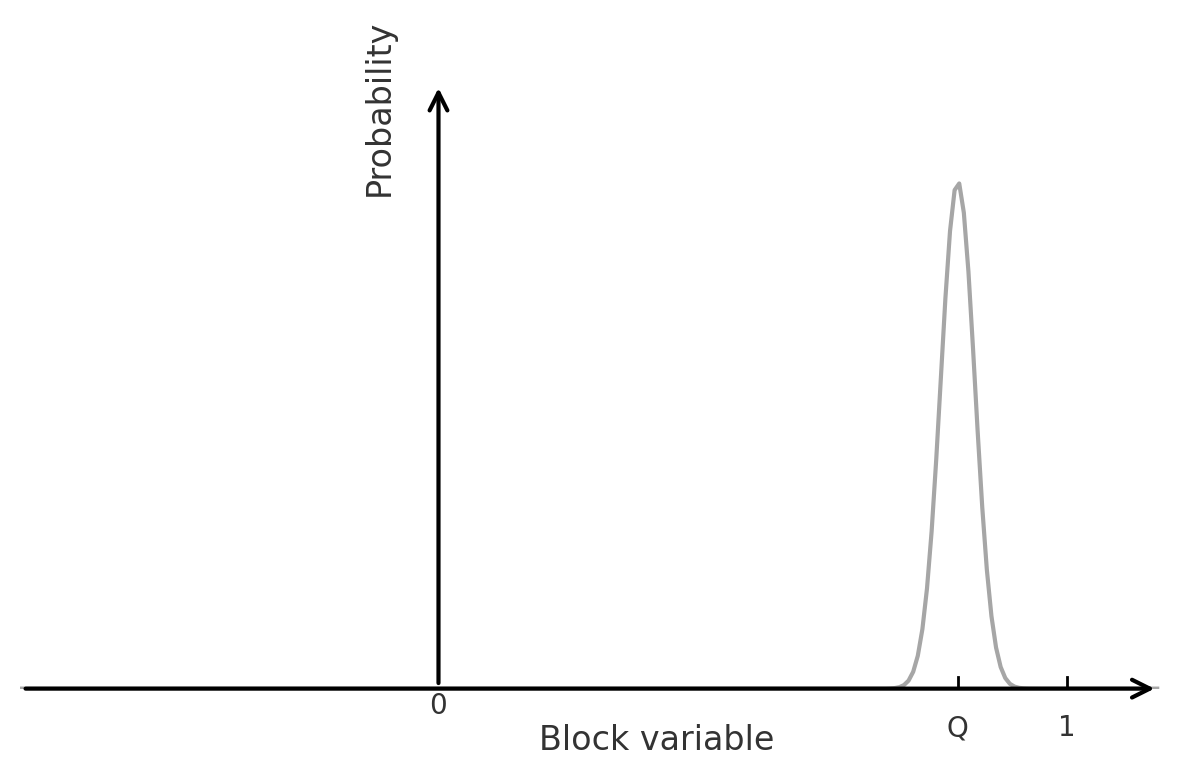
\includegraphics[width=0.84\linewidth,height=\textheight,keepaspectratio]{phase-transitions/Figs/schem_op_ordered.png}

\subcaption{\label{}(biv)}
\end{minipage}%

\caption{\label{fig-c1}See text for details}

\end{figure}%

The results of coarse-graining configurations typical of three different
temperatures are shown in Figure~\ref{fig-c1} and Figure~\ref{fig-c2}.
Two auxiliary operations are implicit in these results. The first
operation is a \emph{length scaling}: the lattice spacing on each
blocked lattice has been scaled to the same size as that of the original
lattice, making possible the display of correspondingly larger portions
of the physical system. The second operation is a \emph{variable
scaling}: loosely speaking, we have adjusted the scale (`contrast') of
the block variable so as to match the spectrum of block variable values
to the spectrum of shades at our disposal.

Consider first a system marginally above its critical point at a
temperature \(T\) chosen so that the correlation length \(\xi\) is
approximately 6 lattice spacing units. A typical arrangement (without
coarse-graining) is shown in Figure~\ref{fig-c1}(ai). The succeeding
figures, Figure~\ref{fig-c1}(aii) and Figure~\ref{fig-c1}(aiii), show
the result of coarse-graining with block sizes \(L=4\) and \(L=8\),
respectively. A clear trend is apparent. The coarse-graining
\emph{amplifies} the consequences of the small deviation of \(T\) from
\(T_c\). As \(L\) is increased, the ratio of the size of the largest
configurational features (\(\xi\)) to the size of the smallest (\(L\))
is reduced. The ratio \(\xi/L\) provides a natural measure of how
`critical' is a configuration. Thus the coarse-graining operation
generates a representation of the system that is effectively less
critical the larger the coarse-graining length. The limit point of this
trend is the effectively fully disordered arrangement shown in
Figure~\ref{fig-c1}(aiii) and in an alternative form in
Figure~\ref{fig-c1}(aiv), which shows the limiting distribution of the
coarse grained variables, averaged over many realizations of the
underlying configurations: the distribution is a Gaussian which is
narrow (even more so the larger the \(L\) value) and centred on zero.
This limit is easily understood. When the system is viewed on a scaled
\(L\) larger than \(\xi\), the correlated microstructure is no longer
explicitly apparent; each coarse-grained variable is essentially
independent of the others.

A similar trend is apparent below the critical point.
Figure~\ref{fig-c1}(bi) show a typical arrangement at a temperature
\(T<T_c\) such that again \(\xi\) is approximately \(6\) lattice
spacings. Coarse-graining with \(L=4\) and \(L=8\) again generates
representations which are effectively less critical
(Figure~\ref{fig-c1}(bii) and (biii)). This time the coarse-graining
smoothes out the microstructure which makes the order incomplete. The
limit point of this procedure is a homogeneously ordered arrangement in
which the block variables have a random (Gaussian) distribution centred
on the order parameter (Figure~\ref{fig-c1}(biv)).

Consider now the situation \emph{at} the critical point.
Figure~\ref{fig-c2}(ai) shows a typical arrangement;
Figure~\ref{fig-c2}(aii) and (aiii) show the results of coarse-graining
with \(L=4\) and \(L=8\) respectively. Since the \(\xi\) is as large as
the system itself the coarse graining does not produce less critical
representations of the physical system: each of the figures displays
structure over \emph{all} length scales between the lower limit set by
\(L\) and the upper limit set by the size of the display itself. A
limiting trend is nevertheless apparent. Although the \(L=4\) pattern is
qualitatively quite different from the pattern of the local variables,
the \(L=4\) and \(L=8\) patterns display qualitatively similar features.
These similarities are more profound than is immediately apparent. A
statistical analysis of the spectrum of \(L=4\) configurations
(generated as the local variables evolve in time) shows
(Figure~\ref{fig-c2}(iv)) that it is almost identical to that of the
\(L=8\) configurations (given the block variable scaling). The
implication of this limiting behaviour is clear: the patterns formed by
the ordering variable at criticality look the same (in a statistical
sense) when viewed on all sufficiently large length scales.

\begin{figure}

\begin{minipage}{0.50\linewidth}

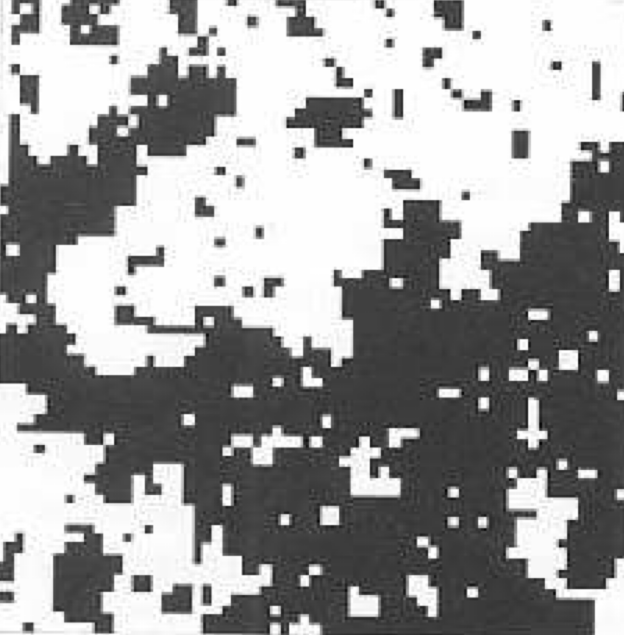
\includegraphics[width=0.5\linewidth,height=\textheight,keepaspectratio]{phase-transitions/Figs/a1_3state.png}

\subcaption{\label{}(ai)}
\end{minipage}%
%
\begin{minipage}{0.50\linewidth}

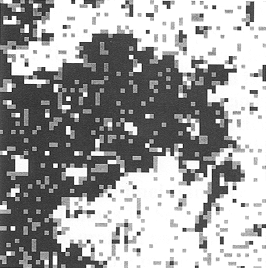
\includegraphics[width=0.5\linewidth,height=\textheight,keepaspectratio]{phase-transitions/Figs/b1_3state.png}

\subcaption{\label{}(bi)}
\end{minipage}%
\newline
\begin{minipage}{0.50\linewidth}

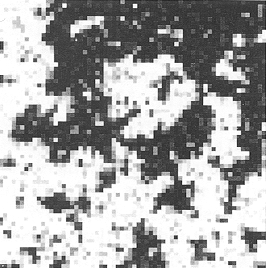
\includegraphics[width=0.5\linewidth,height=\textheight,keepaspectratio]{phase-transitions/Figs/a2_3state.png}

\subcaption{\label{}(aii)}
\end{minipage}%
%
\begin{minipage}{0.50\linewidth}

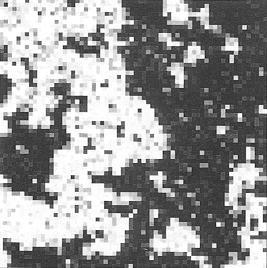
\includegraphics[width=0.5\linewidth,height=\textheight,keepaspectratio]{phase-transitions/Figs/b2_3state.png}

\subcaption{\label{}(bii)}
\end{minipage}%
\newline
\begin{minipage}{0.50\linewidth}

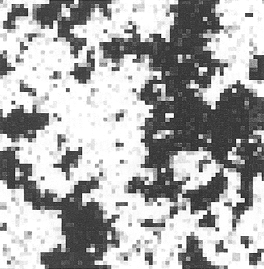
\includegraphics[width=0.5\linewidth,height=\textheight,keepaspectratio]{phase-transitions/Figs/a3_3state.png}

\subcaption{\label{}(aiii)}
\end{minipage}%
%
\begin{minipage}{0.50\linewidth}

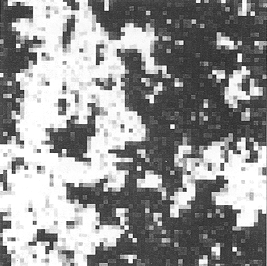
\includegraphics[width=0.5\linewidth,height=\textheight,keepaspectratio]{phase-transitions/Figs/b3_3state.png}

\subcaption{\label{}(biii)}
\end{minipage}%
\newline
\begin{minipage}{\linewidth}

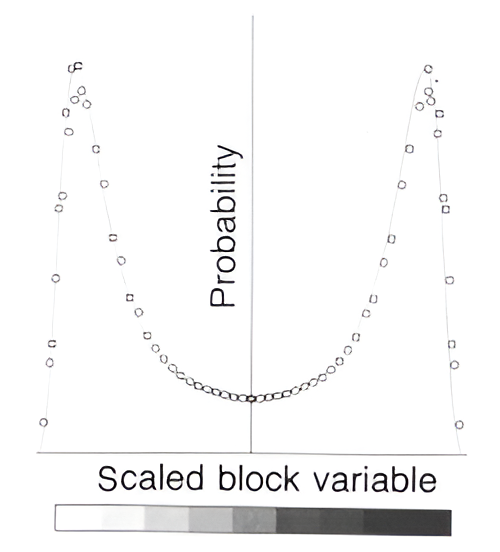
\includegraphics[width=0.5\linewidth,height=\textheight,keepaspectratio]{phase-transitions/Figs/scaled_block_variable.png}

\subcaption{\label{}(iv)}
\end{minipage}%

\caption{\label{fig-c2}See text for details}

\end{figure}%

Let us summarize. Under the coarse-graining operation there is an
evolution or \emph{flow} of the system's configuration spectrum. The
flow tends to a limit, or fixed point, such that the pattern spectrum
does not change under further coarse-graining. These scale-invariant
limits have a trivial character for \(T>T_c\), (a perfectly disordered
arrangement) and \(T< T_c\), (a perfectly ordered arrangement). The
hallmark of the critical point is the existence of a scale-invariant
limit which is neither fully ordered nor fully disordered but which
possesses structure on all length scales. A nice illustration of
critical point scale invariance in the Ising model can be viewed
\href{https://www.youtube.com/watch?v=fi-g2ET97W8&ab_channel=DouglasAshton}{here}.

\section{Universality and Scaling}\label{universality-and-scaling}

Equipped with the coarse-graining technique, we now address the
universality phenomenon. We aim to understand how it is that systems
that are different microscopically can nevertheless display critical
point behaviour which (in certain respects) is quantitatively identical.

To obtain initial insight we introduce a spin-1 Ising model in which the
spins take on three values (\(s_i=1,0,-1\)), in contrast to the two
values (\(s_i=1,-1\)) of the spin-1/2 Ising model. The two models have
properties which are different: for example, \(T_c\) for the three-state
model is some \(30\%\) lower than that of the two-state model (for the
same coupling \(J\)). However, there is abundant evidence that the two
models have the same universal properties.

Let us explore what is the same and what is different in the
configurations of the two models at criticality. The configurations of
the local variables \(s_i\) are clearly qualitatively different for the
two models. Now consider the coarse-grained configurations (with \(L=4\)
and \(L=8\) respectively) for the three-state model at the critical
point. We have already seen that the coarse-graining operation bears the
configuration spectrum of the critical two-state Ising model to a
non-trivial scale-invariant limit. It is scarcely surprising that the
same is true for the three-state model. What is remarkable is that the
two limits are the same! This is expressed in Figure~\ref{fig-c2}(iv),
which shows the near coincidence of the distribution of block variables
(grey-levels) for the two different coarse-graining lengths. Thus the
coarse-graining erases the physical differences apparent in
configurations where the local behaviour is resolvable, and exposes a
profound configurational similarity.

\subsection{Fluid-magnet universality}\label{fluid-magnet-universality}

Let us now turn to fluid-magnet universality. In a magnet, the relevant
configurations are those formed by the coarse-grained magnetisation (the
magnetic moment averaged over a block of side \(L\)). In a fluid, the
relevant configurations are those of the coarse-grained density (the
mass averaged over a block if side \(L\)) or more precisely, its
fluctuation from its macroscopic average (Figure~\ref{fig-fmcoarse}).
The patterns in the latter (bubbles of liquid or vapour) may be matched
to pattern in the former (microdomains of the magnetisation), given
appropriate scaling operations to camouflage the differences between the
length scales and the differences between the variable scales.

\begin{figure}

\centering{

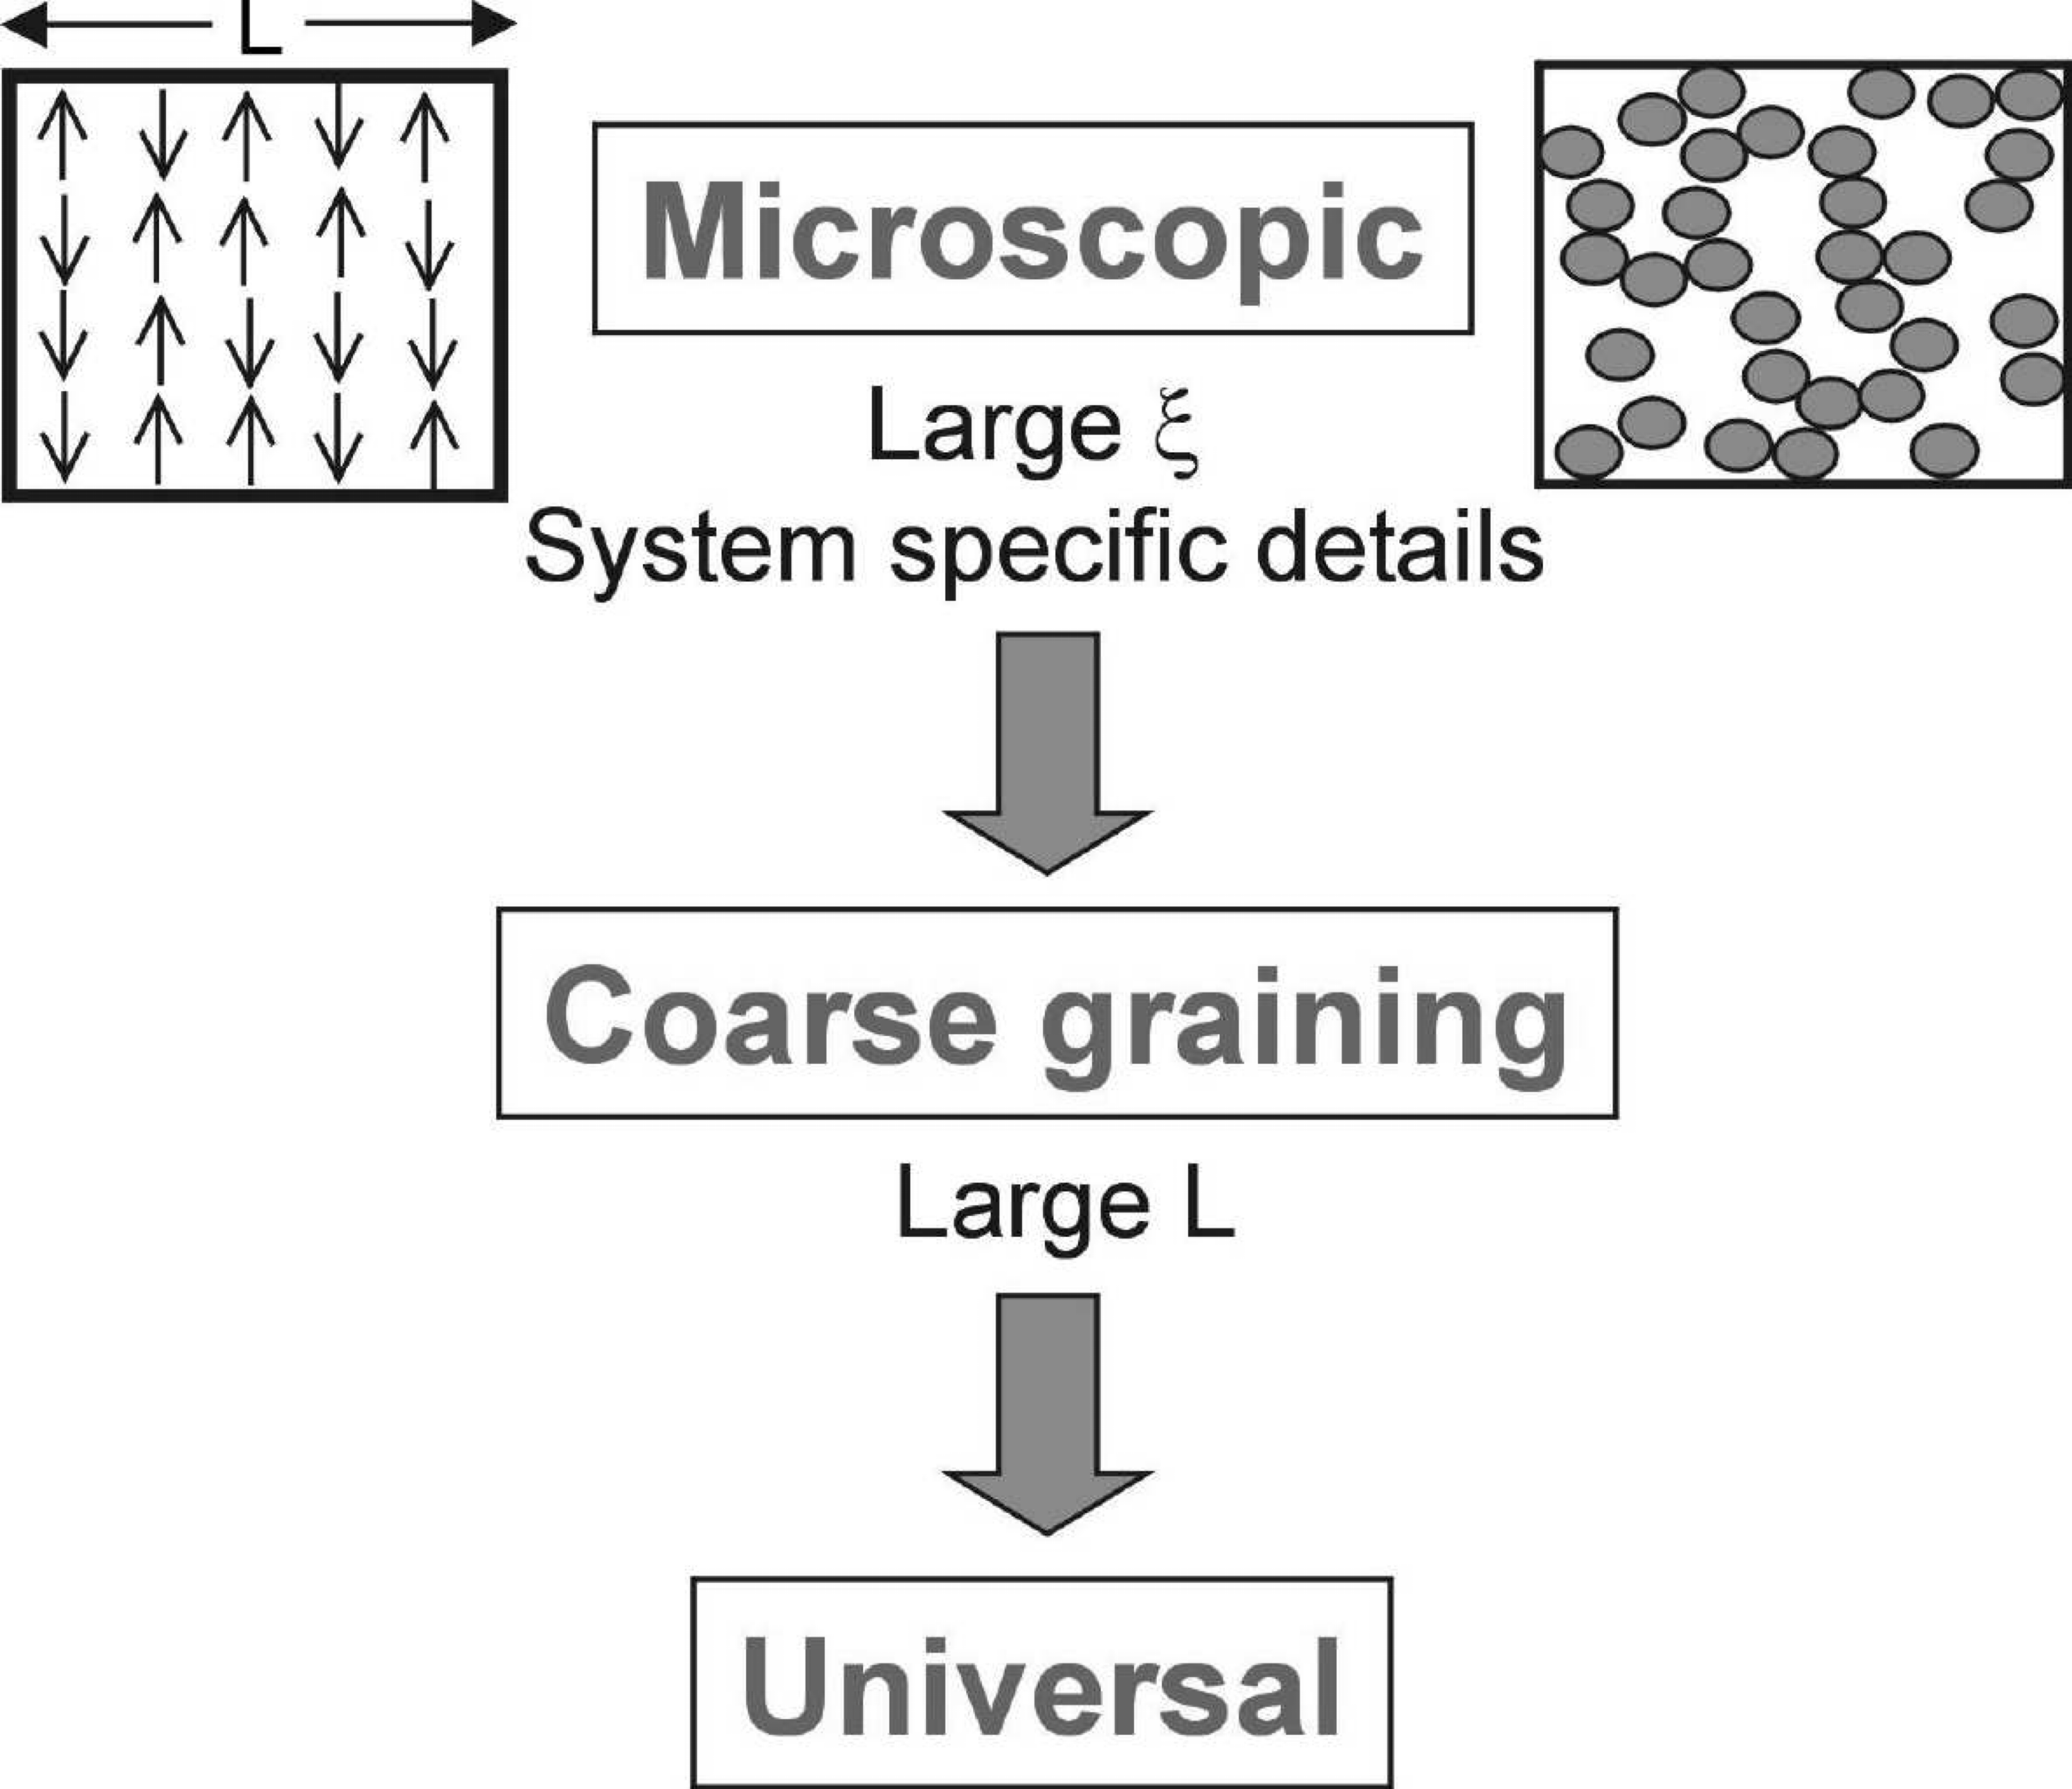
\includegraphics[width=0.5\linewidth,height=\textheight,keepaspectratio]{phase-transitions/Figs/coarse.png}

}

\caption{\label{fig-fmcoarse}Schematic representation of the coarse
graining operation via which the universal properties of fluids and
magnets may be exposed.}

\end{figure}%

The results is illustrated in Figure~\ref{fig-confscomp}.

\begin{figure}

\begin{minipage}{\linewidth}

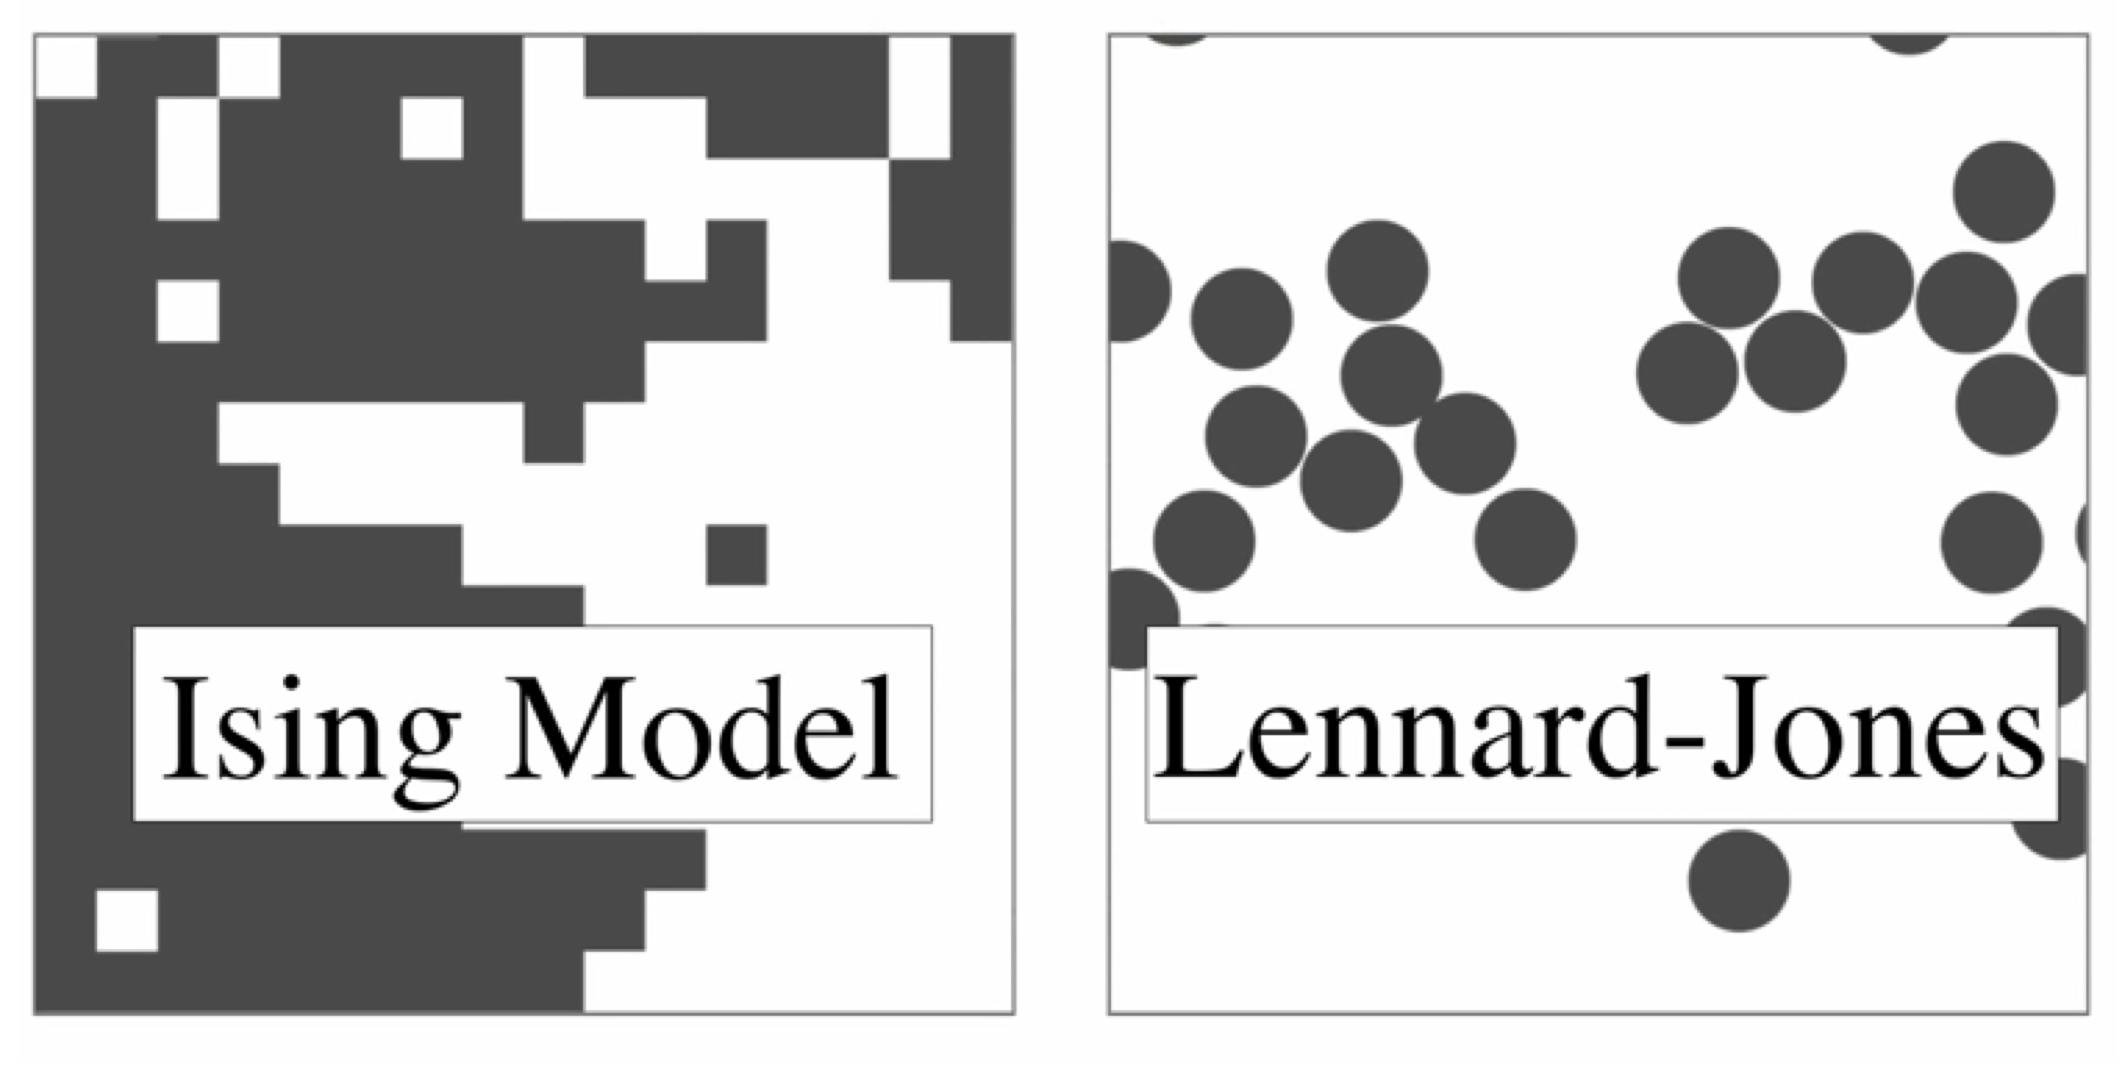
\includegraphics[width=0.5\linewidth,height=\textheight,keepaspectratio]{phase-transitions/Figs/fluid-magnet.png}

\subcaption{\label{}2D critical Ising model and 2d critical
Lennard-Jones fluid at small lengthscales}
\end{minipage}%
\newline
\begin{minipage}{\linewidth}

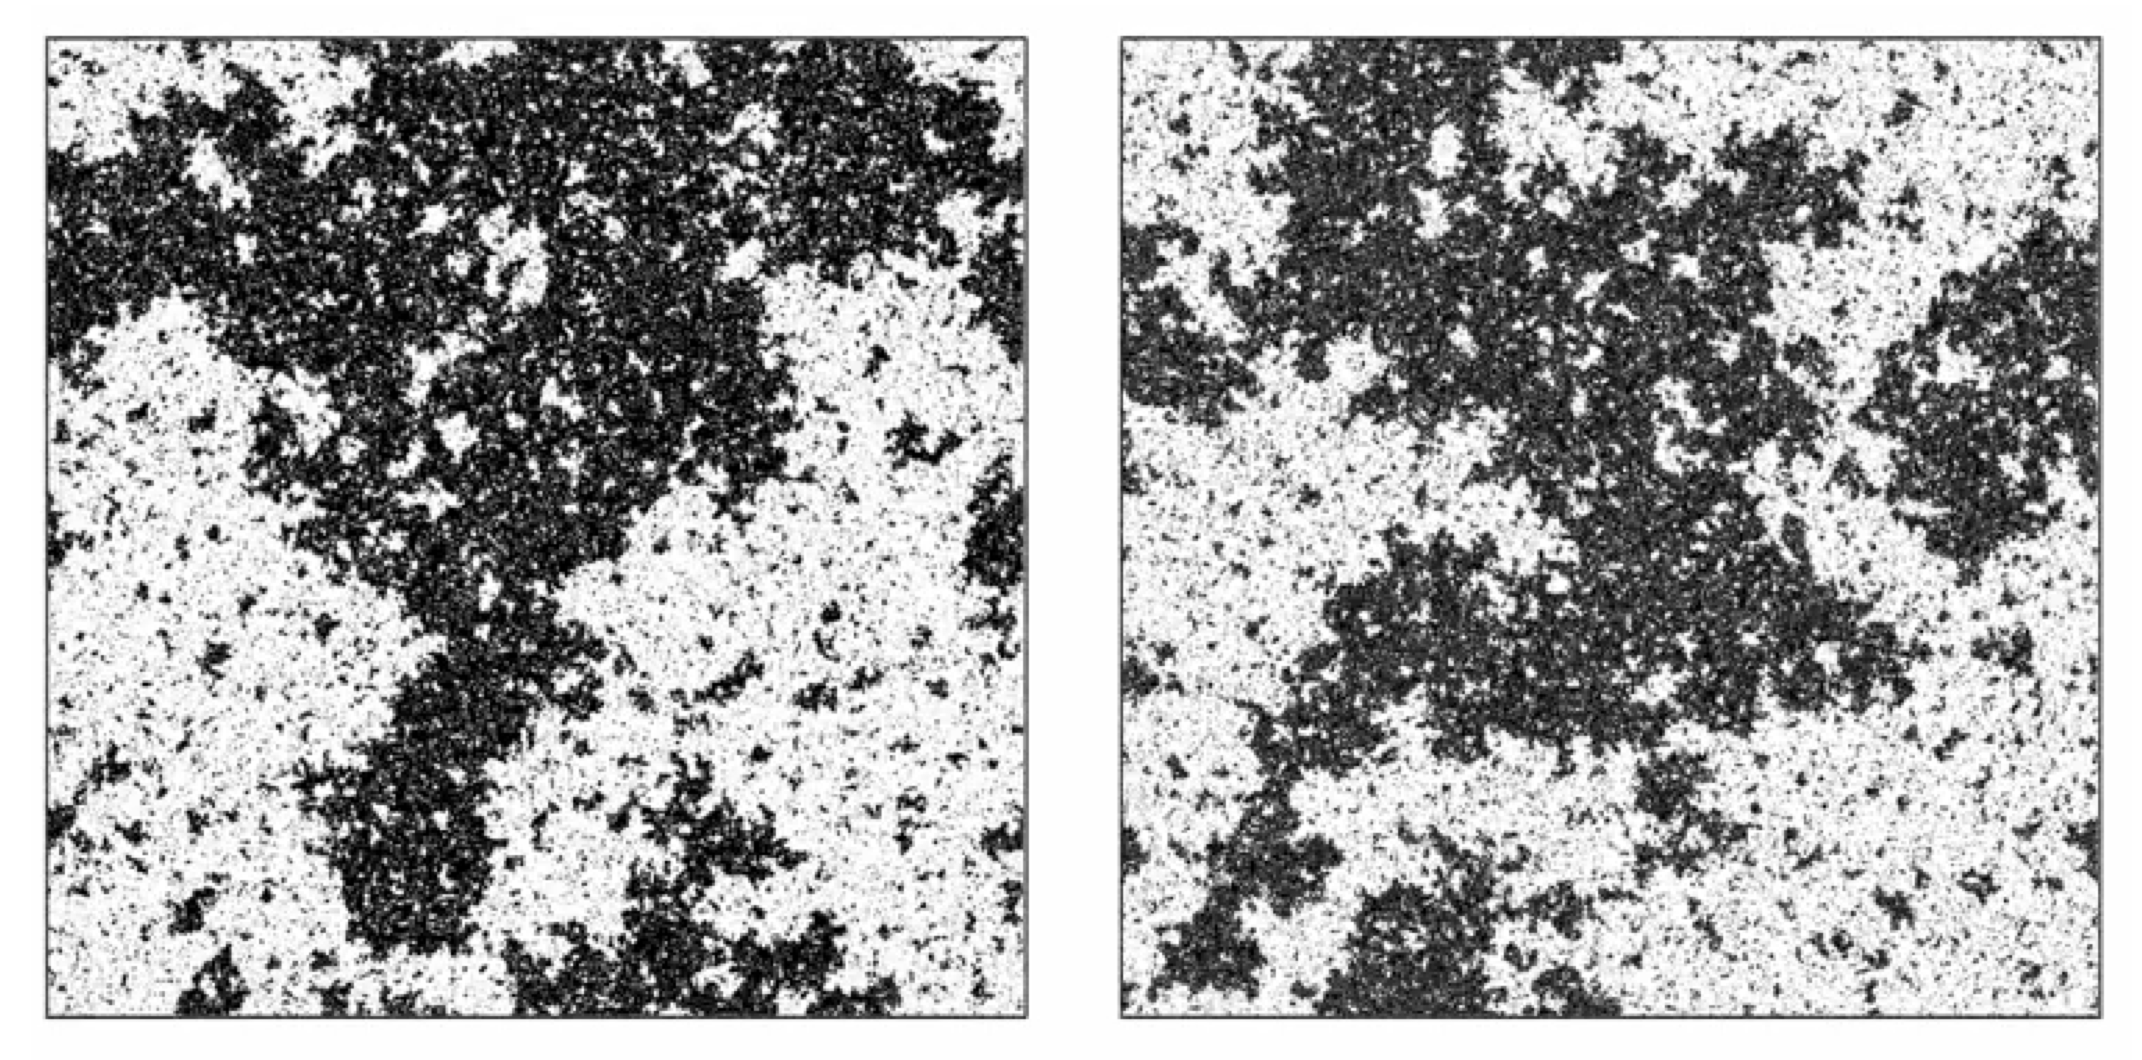
\includegraphics[width=0.5\linewidth,height=\textheight,keepaspectratio]{phase-transitions/Figs/fluid-magnet2.png}

\subcaption{\label{}Same models as above, but viewed at large
lengthscales}
\end{minipage}%

\caption{\label{fig-confscomp}Snapshot configurations of the 2D critical
Ising model (left) and the 2D critical Lennard-Jones fluid (right). When
viewed on sufficiently large length scales the configurational patterns
appear universal and self similar.}

\end{figure}%

A movie in which we progressively zoom out shows how the loss of
microscopic details reveals the large lengthscale universal features.
\url{Movies/universality.mov}

\section{Near critical scaling}\label{near-critical-scaling}

The similarity of coarse-grained configurations of different systems is
not restricted to the critical temperature itself. Suppose we have a two
state spin model and a three state spin model each somewhat above their
critical points at reduced temperature \(t\). The two systems will have
somewhat different correlation lengths, \(\xi_1\) and \(\xi_2\) say.
Suppose however, we choose coarse-graining lengths \(L_1\) for \(L_2\)
for the two models such that \(\xi_1/L_1=\xi_2/L_2\). We adjust the
scales of the block variables (our grey level control) so that the
typical variable value is the same for the two systems. We adjust the
length scale of the systems (stretch or shrink our snapshots) so that
the sizes of the minimum-length-scale structure (set by \(L_1\) and
\(L_2\)) looks the same for each system. Precisely what they look like
depends upon our choice of \(\xi/L\).

\section{Universality classes}\label{sec-unipics}

Coarse graining does not erase all differences between the physical
properties of critical systems. Differences in the space dimension \(d\)
of two critical systems will lead to different universal properties such
as critical exponents. Thus, for instance, the critical exponents of the
2D magnet, match those of the 2d fluid, but they are different to those
of 3d magnets and fluids.

\begin{longtable}[]{@{}
  >{\raggedright\arraybackslash}p{(\linewidth - 4\tabcolsep) * \real{0.4062}}
  >{\raggedright\arraybackslash}p{(\linewidth - 4\tabcolsep) * \real{0.2969}}
  >{\raggedright\arraybackslash}p{(\linewidth - 4\tabcolsep) * \real{0.2969}}@{}}
\toprule\noalign{}
\begin{minipage}[b]{\linewidth}\raggedright
\end{minipage} & \begin{minipage}[b]{\linewidth}\raggedright
\(d=2\)
\end{minipage} & \begin{minipage}[b]{\linewidth}\raggedright
\(d=3\)
\end{minipage} \\
\midrule\noalign{}
\endhead
\bottomrule\noalign{}
\endlastfoot
Critical temperature & 0.5673 & 0.75 \\
Order parameter exponent \(\beta\) & \(\tfrac{1}{8}\) &
\(0.325 \pm 0.001\) \\
Susceptibility exponent \(\gamma\) & \(\tfrac{7}{4}\) &
\(1.24 \pm 0.001\) \\
Correlation length exponent \(\nu\) & \(1\) & \(0.63 \pm 0.001\) \\
\end{longtable}

In fact the space dimension is one of a small set of qualitative
features of a critical system which are sufficiently deep-seated to
survive coarse graining and which together serve to define the system's
universal behaviour, or \emph{universality class}. The constituents of
this set are not all identifiable \emph{a priori}. They include the
number of components \(n\) of the order parameter. Up to now, we have
only considered order parameters which are scalar (for a fluid the
density, for a magnet the magnetisation), for which \(n=1\). In some
ferromagnets, the order parameter may have components along two axes, or
three axes, implying a vector order parameter, with \(n=2\) (the
solcalled XY model) or \(n=3\) (Heisenberg model), respectively. It is
clear that the order-parameter \(n\)-value will be reflected in the
nature of the coarse-grained configurations, and thus in the universal
observables they imply.

A third important feature which can change the universality class of a
critical system is the range of the interaction potential between its
constituent particles. Clearly for the Ising model, interactions between
spins are inherently nearest neighbour in character. Most fluids
interact via dispersion forces (such as the Lennard-Jones potential)
which is also short ranged owing to the \(r^{-6}\) attractive
interaction. However some systems have much longer ranged interactions.
Notable here are systems of charged particles which interact via a
Coulomb potential. The long ranged nature of the Coulomb potential
(which decays like \(r^{-1}\)) means that charged systems often do not
have the same critical exponents as the Ising model and fluid.

\section{Critical exponents}\label{critical-exponents}

We consider now how the critical exponents, may be computed via the
coarse-graining procedure. In what follows we will refer only to the
behaviour of a single typical coarse grained variable, which we shall
denote \(S(L)\). We suppose that \(t\) is sufficiently small that
\(\xi \gg
L_\textrm{ min}\). Universality and scaling may be expressed in the
claim that, for \emph{any} \(L\) and \(t\), scale factors \(a(L)\) and
\(b(L)\) may be found such that the probability distribution
\(p(S(L),t)\) can be written in the form

\begin{equation}\phantomsection\label{eq-blocks}{
p(S(L),t)=b(L)\tilde{p}(b(L)S(L),a(L)t)
}\end{equation} where \(\tilde{p}\) is a function unique to a
universality class. The role of the scale factors \(a\) and \(b\) is to
absorb the basic non-universal scales identified in
Section~\ref{sec-rgmethod}. The critical exponents are implicit in the
\(L\)-dependence of these scale factors. Specifically one finds:

\begin{equation}\phantomsection\label{eq-scalefacs}{
\begin{aligned}
a(L) & =a_0L^{1/\nu} \\
b(L) & =b_0L^{\beta/\nu}
\end{aligned} 
}\end{equation} where the amplitudes \(a_0\) and \(b_0\) are system
specific (non-universal) constants.

These results state that the critical exponents (in the form \(1/\nu\)
and \(\beta/\nu\)) characterize the ways in which the configuration
spectrum evolves under coarse-graining. Consider, first the exponent
ratio \(\beta/\nu\). Precisely at the critical point, there is only one
way in which the coarse-grained configurations change with \(L\): the
overall scale of the coarse-grained variable (the black-white contrast
in our grey scale representation) is eroded with increasing \(L\). Thus
the configurations of coarse-graining length \(L_1\) match those of a
larger coarse-graining length \(L_2\) only if the variable scale in the
latter configurations is amplified. The required amplification follows
from Equation~\ref{eq-blocks} and and Equation~\ref{eq-scalefacs}: it is

\[
\frac{b(L_2)}{b(L_1)}=\left(\frac{L_2}{L_1}\right)^{\beta/\nu}\:.
\] The exponent ratio \(\beta/\nu\) thus controls the rate at which the
scale of the ordering variable decays with increasing coarse-graining
length.

Consider now the exponent \(1/\nu\). For small but non-zero reduced
temperature (large but finite \(\xi\)) there is second way in which the
configuration spectrum evolves with \(L\). As noted previously, coarse
graining reduces the ratio of correlation length to coarse-graining
length, and results in configurations with a less critical appearance.
More precisely, we see from Equation~\ref{eq-blocks} that increasing the
coarse graining length from \(L_1\) to \(L_2\) while keeping the reduced
temperature constant has the same effect on the configuration spectrum
as keeping coarse-graining length constant which amplifying the reduced
temperature \(t\) by a factor

\[
\frac{a(L_2)}{a(L_1)}=\left(\frac{L_2}{L_1}\right)^{1/\nu}\:.
\] One may think of the combination \(a(L)t\) as a measure of the
effective reduced temperature of the physical system viewed with
resolution length \(L\). The exponent \(1/\nu\) controls the rate at
which the effective reduced temperature flows with increasing
coarse-graining length.

\section{Finite-size scaling}\label{sec-fss}

We can exploit the fact that the scale factors \(a(L)\) and \(b(L)\)
depend on critical exponents to estimate the values of these exponents
using computer simulation. Consider the average of the block variable
\(S(L)\). Consideration of Equation~\ref{eq-blkvar} shows that this is
non other than the value of the order parameter \(Q\), measured over a
block of side \(L\). Thus from the definition of an average

\[
Q(L,t)=\bar {S}(L,t)=\int S(L)p(S(L),t)dS(L)
\] where \(p(S(L))\) is the probability distribution of \(S(L)\).

Making use of the representation of Equation~\ref{eq-blocks}, we then
have that

\[Q
(L,t) = \int b(L)S(L)\tilde{p}(b(L)S(L),a(L)t)dS(L)
\]

To integrate this we need to change the integration variable from
\(S(L)\) to \(b(L)S(L)\). We have \(d(b(L)S(L))=b(L)dS(L)\) since
\(b(L)\) does not fluctuate. Thus \[
\begin{aligned}
Q(L,t)  & =  b^{-1}(L)\int b(L)S(L)\tilde{p}(b(L)S(L),a(L)t)d(b(L)S(L))\nonumber\\
        & =  b^{-1}(L)f(a(L)t)\nonumber\\
       & =  b_0L^{-\beta/\nu}f(a_0L^{1/\nu}t)
\end{aligned}
\]

where \(f\) is a universal function (defined as the first moment of
\(\tilde{p}(x,y)\) with respect to \(y\)).

The above results provide a method for determining the critical exponent
ratios \(\beta/\nu\) and \(1/\nu\) via computer simulations of near
critical systems. For instance, at the critical point (\(t=0\)) and for
finite block size, \(Q(L,0)\) will not be zero (the \(T\) at which Q
vanishes for finite \(L\) is above the true \(T_c\), cf.
Section~\ref{sec-compsim}. However, we know that its value must vanish
in the limit of infinite \(L\); it does so like

\[Q(L,0)=b_0L^{-\beta/\nu}f(0)\equiv Q_0L^{-\beta/\nu}\]

Thus by studying the critical point \(L\) dependence of \(Q\) we can
estimate \(\beta/\nu\). A similar approach in which we study two block
sizes \(L\), and tune \(t\) separately in each case so that the results
for \(QL^{\beta/\nu}\) are identical provides information on the value
of \(1/\nu\).

\section{Summary of main points}\label{summary-of-main-points}

As this is quite a long chapter let us summarise the main points:

\begin{itemize}
\item
  \textbf{Limitations of conventional theories}: Mean field theories and
  the scaling hypothesis are insufficient in the critical region due to
  their neglect of correlations across all relevant length scales.
\item
  \textbf{Critical region characteristics}: Near-critical systems
  exhibit correlated microstructure on all length scales up to the
  correlation length. The complexity of this structure makes both
  analytical and computational study challenging.
\item
  \textbf{Relevant length scales}:

  \begin{enumerate}
  \def\labelenumi{\arabic{enumi}.}
  \tightlist
  \item
    Correlation length (\(\xi\))
  \item
    Minimum microscopic scale (\(L_\textrm{min}\))
  \item
    Macroscopic system size (\(L_\textrm{max}\))
  \end{enumerate}
\item
  \textbf{Window Condition for criticality}: The true critical regime
  satisfies \(L_\textrm{max} \gg \xi \gg L_\textrm{min}\), encompassing
  a broad range of scales where complex, often fractal-like, structures
  are present.
\item
  \textbf{Renormalisation Group (RG) methodology}: RG involves the
  stepwise elimination of degrees of freedom by coarse-graining the
  system over increasing length scales. A fourth scale, \(L\),
  represents the resolution at which the system is described.
\item
  \textbf{Effect of coarse-graining}: Coarse-graining changes the
  effective reduced temperature, captured by the relation \(a(L)t\),
  where \(a(L)\) scales with \(L\) as \(L^{1/\nu}\). This helps describe
  how critical configurations evolve with resolution.
\item
  \textbf{Universality}:

  \begin{itemize}
  \tightlist
  \item
    Coarse-graining reveals that microscopically different systems can
    exhibit identical critical behavior when observed at large scales.
  \item
    The concept of universality explains why disparate systems, such as
    magnets and fluids, can show the same critical exponents and scaling
    laws.
  \item
    Critical behavior depends primarily on general features like
    dimensionality and symmetry, rather than microscopic details.
  \end{itemize}
\item
  \textbf{Finite-Size scaling}:

  \begin{itemize}
  \tightlist
  \item
    The average block variable \(Q(L,t)\) is related to block size \(L\)
    and reduced temperature \(t\) through scaling relations. Computer
    simulations exploit this to extract scaling functions and the values
    of critical exponents.
  \end{itemize}
\end{itemize}

\section{Addendum: The effective coupling viewpoint of the
renormalization group (non
examinable)}\label{addendum-the-effective-coupling-viewpoint-of-the-renormalization-group-non-examinable}

\begin{tcolorbox}[enhanced jigsaw, toprule=.15mm, opacityback=0, colbacktitle=quarto-callout-caution-color!10!white, title=\textcolor{quarto-callout-caution-color}{\faFire}\hspace{0.5em}{Notes for those interested in a different perspective on RG theory.}, leftrule=.75mm, rightrule=.15mm, bottomtitle=1mm, breakable, colframe=quarto-callout-caution-color-frame, colback=white, toptitle=1mm, left=2mm, titlerule=0mm, coltitle=black, arc=.35mm, bottomrule=.15mm, opacitybacktitle=0.6]

Let us begin by returning to our fundamental Equation~\ref{eq-probs},
which we rewrite as

\[p = Z^{-1}e^{-{\cal H}}\] where \({\cal H}\equiv E/k_BT\).

The first step is then to imagine that we generate, by a computer
simulation procedure for example, a sequence of configurations with
relative probability \(\exp(-{\cal H})\). We next adopt some
coarse-graining procedure which produces from these original
configurations a set of coarse-grained configurations. We then ask the
question: what is the energy function \({\cal H}^\prime\) of the
coarse-grained variables which would produce these coarse-grained
configurations with the correct relative probability
\(\exp(-{\cal H}^\prime)\)? Clearly the form of \({\cal H}^\prime\)
depends on the form of \({\cal H}\) thus we can write symbolically

\[{\cal H}^\prime=R({\cal H})\]

The operation \(R\), which defines the coarse-grained configurational
energy in terms of the microscopic configurational energy function is
known as a renormalisation group transformation (RGT). What it does is
to replace a hard problem by a less hard problem. Specifically, suppose
that our system is near a critical point and that we wish to calculate
its large-distance properties. If we address this task by utilizing the
configurational energy and appealing to the basic machinery of
statistical mechanics set out in Equation~\ref{eq-probs} and
Equation~\ref{eq-partition}, the problem is hard. It is hard because the
system has fluctuations on all the (many) length scales intermediate
between the correlation length \(\xi\) and the minimum length scale
\(L_\textrm{min}\).

However, the task may instead be addressed by tackling the
coarse-grained system described by the energy \({\cal H}^\prime\). The
large-distance properties of this system are the same as the
large-distance properties of the physical system, since coarse-graining
operation preserves large-scale configurational structure. In this
representation the problem is a little easier: while the \(\xi\)
associated with \({\cal H}^\prime\) is the same as the \(\xi\)
associated with \({\cal H}\), the minimum length scale of
\({\cal H}^\prime\) is bigger than that of \({\cal H}\). Thus the
statistical mechanics of \({\cal H}^\prime\) poses a
not-quite-so-many-length-scale problem, a problem which is effectively a
little less critical and is thus a little easier to solve. The benefits
accruing from this procedure may be amplified by repeating it. Repeated
application of \(R\) will eventually result in a coarse- grained energy
function describing configurations in which the \(\xi\) is no bigger
than the minimum length scale. The associated system is far from
criticality and its properties may be reliably computed by any of a wide
variety of approximation schemes. These properties are the desired
large-distance properties of the physical system. As explicit reference
to fluctuations of a given scale is eliminated by coarse-graining, their
effects are carried forward implicitly in the parameters of the
coarse-grained energy.

In order to setup the framework for a simple illustrative example, let
is return to the lattice Ising model for which the energy function
depended only on the product of nearest neighbour spins. The coefficient
of this product in the energy is the exchange coupling, \(J\). In
principle, however, other kinds of interactions are also allowed; for
example, we may have a product of second neighbour spins with strength
\(J_2\) or, perhaps, a product of four spins (at sites forming a square
whose side is the lattice spacing), with strength \(J_3\). Such
interactions in a real magnet have their origin in the quantum mechanics
of the atoms and electrons and clearly depend upon the details of the
system. For generality therefore we will allow a family of exchange
couplings \(J_1\),\(J_2\),\(J_3,\dots\), or \(J_a, a =
1,2,\dots\) In reduced units, the equivalent coupling strengths are
\(K_a =J_a/k_BT\). Their values determine uniquely the energy for any
given configuration.

\begin{quote}
We note that it is not only useful to allow for arbitrary kinds of
interactions: if we wish to repeat the transformation several (indeed
many) times, it is also necessary because even if we start with only the
nearest neighbour coupling in \({\cal H}\) the transformation will in
general produce others in \({\cal H}^\prime\).
\end{quote}

Now consider the coarse-graining procedure. Let us suppose that this
procedure takes the form of a `majority rule' operation in which the new
spins are assigned values \(+1\) or \(-1\) according to the signs of the
magnetic moments of the blocks with which they are associated. The new
energy function \({\cal H}^\prime\) will be expressible in terms of some
new coupling strengths \(K^\prime\) describing the interactions amongst
the new spin variables (and thus, in effect, the interactions between
blocks of the original spin variables). The RGT simply states that these
new couplings depend on the old couplings: \(K_1^\prime\) is some
function \(f_1\) of all the original couplings, and generally

\begin{equation}\phantomsection\label{eq-rgt}{K^\prime_a=f_a(K_1,K_2,\dots) =f_a({\bf K}),~~~~ a= 1, 2,\dots
}\end{equation} where \textbf{K} is shorthand for the set
\(K_1, K_2,\dots\)

\subsection{A simple example}\label{a-simple-example}

This example illustrates how one can perform the RG transformation
Equation~\ref{eq-rgt} directly, without recourse to a `sequence of
typical configurations'. The calculation involves a very crude
approximation which has the advantage that it simplifies the subsequent
analysis.

\begin{figure}[H]

\centering{

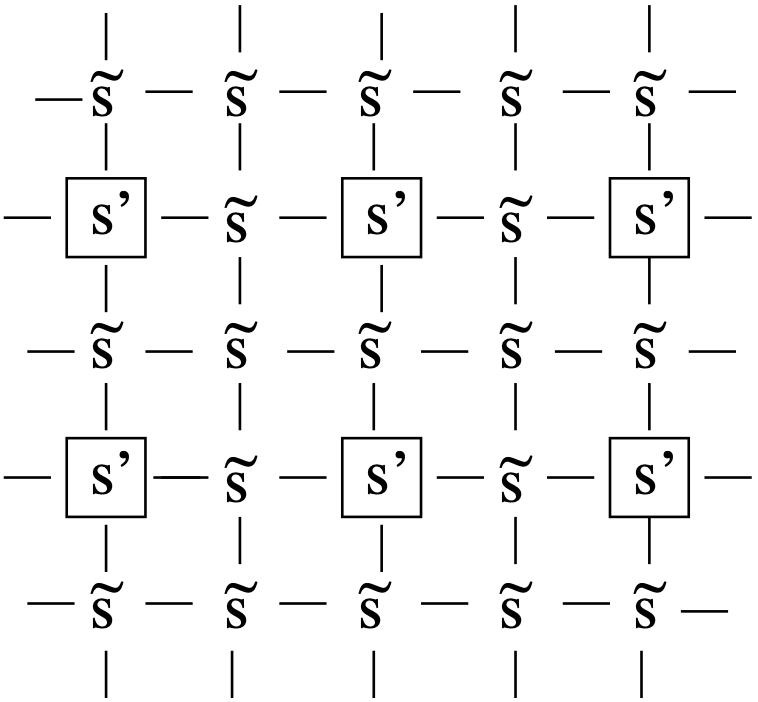
\includegraphics[width=0.4\linewidth,height=\textheight,keepaspectratio]{phase-transitions/Figs/rglat.png}

}

\caption{\label{fig-rglat}Coarse graining by decimation. The spins on
the original lattice are divided into two sets \(\{s^\prime\}\) and
\(\{\tilde{s}\}\). The \(\{s^\prime\}\) spins occupy a lattice whose
spacing is twice that of the original. The effective coupling
interaction between the \(\{s^\prime\}\) spins is obtained by performing
the configurational average over the \(\{\tilde{s}\}\)}

\end{figure}%

Consider an Ising model in two dimensions, with only nearest neighbour
interactions as shown in Figure~\ref{fig-rglat}. We have divided the
spins into two sets, the spins \(\{s^\prime\}\) form a square lattice of
spacing \(2\), the others being denoted by \(\{\tilde{s}\}\). One then
defines an effective energy function \({\cal H^\prime}\) for the
\(s^\prime\) spins by performing an average over all the possible
arrangements of the \(\tilde{s}\) spins

\begin{equation}\phantomsection\label{eq-decimate}{
\exp(-{\cal H}^\prime)=\sum_{\{\tilde {s}\}} \exp(-{\cal H}).
}\end{equation}

This particular coarse-graining scheme is called `decimation' because a
certain fraction (not necessarily one-tenth!) of spins on the lattice is
eliminated. This formulation of a new energy function realizes two basic
aims of the RG method: the long-distance physics of the `original'
system, described by \({\cal H}\), is contained in that of the `new'
system, described by \({\cal H}^\prime\) (indeed the partition functions
are the same as one can see by summing both sides over \(s^\prime\)) and
the new system is further from critically because the ratio of \(\xi\)
to lattice spacing (`minimum length scale') has been reduced by a factor
of \(1/2\) (the ratio of the lattice spacings of the two systems). We
must now face the question of how to perform the configuration sum in
Equation~\ref{eq-decimate}. This cannot in general be done exactly, so
we must resort to some approximation scheme. The particular
approximation which we invoke is the high temperature series expansion.
In its simplest mathematical form, since \({\cal H}\) contains a factor
\(1/k_BT\), it involves the expansion of \(\exp(-{\cal H})\) as a power
series:

\[\exp(-{\cal H}/k_BT)=1-{\cal H}/k_BT +\frac{1}{2!}({\cal H}/k_BT)^2+.....\]

We substitute this expansion into the right hand side of
Equation~\ref{eq-decimate} and proceed to look for terms which depend on
the \(s^\prime\) spins after the sum over the possible arrangements of
the \(\tilde{s}\) spins is performed. This sum extends over all the
possible (\(\pm 1\)) values of all the \(\tilde{s}\) spins. The first
term (the 1) in the expansion of the exponential is clearly independent
of the values of the \(s^\prime\) spins. The second term (\({\cal H}\))
is a function of the \(s^\prime\) spins, but gives zero when the sum
over the \(s^\prime\) spins is performed because only a single factor of
any \(s^\prime\) ever appears, and \(+ 1 - 1 = 0\). The third term
(\({\cal H}^2/2\)) does contribute. If one writes out explicitly the
form of \({\cal H}^2/2\) one finds terms of the form
\(K^2s_1^\prime\tilde{s}\tilde{s}s_2^\prime=K^2s_1^\prime s_2^\prime\),
where \(s_1^\prime\) and \(s_2^\prime\) denote two spins at nearest
neighbour sites on the lattice of \(s^\prime\) spins and \(\tilde{s}\)
is the spin (in the other set) which lies between them. Now, in the
corresponding expansion of the left hand side of
Equation~\ref{eq-decimate}, we find terms of the form
\(K^\prime s_1^\prime s_2^\prime\), where \(K^\prime\) is the nearest
neighbour coupling for the \(s^\prime\) spins. We conclude (with a
little more thought than we detail here) that

\begin{equation}\phantomsection\label{eq-rgdec}{
K^\prime=K^2
}\end{equation}

Of course many other terms and couplings are generated by the higher
orders of the high temperature expansion and it is necssary to include
these if one wishes reliable values for the critical temperature and
exponents, However, our aim here is to use this simple calculation to
illustrate the RG method. Let us therefore close our eyes, forget about
the higher order terms and show how the RGT Equation~\ref{eq-rgdec} can
be used to obtain information on the phase transition.

\begin{figure}[H]

\centering{

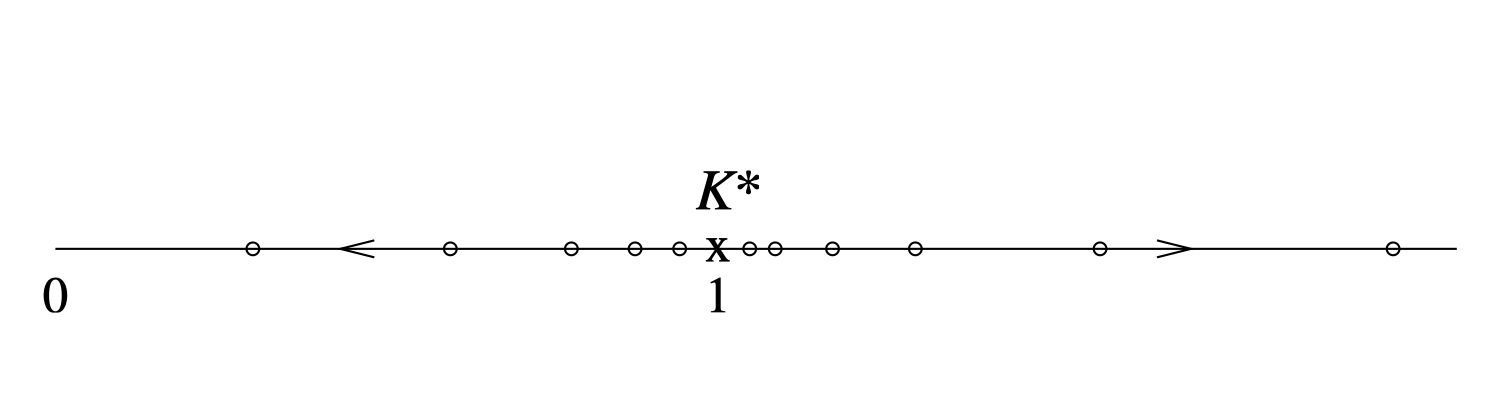
\includegraphics[width=0.6\linewidth,height=\textheight,keepaspectratio]{phase-transitions/Figs/flow1.png}

}

\caption{\label{fig-flow1}Coupling flow under the decimation
transformation described in the text.}

\end{figure}%

The first point to note is that that mathematically
Equation~\ref{eq-rgdec} has the fixed point \(K^*= 1\); if \(K= 1\) then
the new effective coupling \(K^\prime\) has the same value \(1\).
Further, if \(K\) is just larger than \(1\), then \(K^\prime\) is larger
than \(K\), i.e.~further away from \(1\). Similarly, if \(K\) is less
than \(1\), \(K^\prime\) is less than \(K\). We say that the fixed point
is unstable: the flow of couplings under repeated iteration of
Equation~\ref{eq-rgdec} is away from the fixed point, as illustrated in
Figure~\ref{fig-flow1}. The physical significance of this is as follows:
suppose that the original system is at its critical point so that the
ratio of \(\xi\) to lattice spacing is infinite. After one application
of the decimation transformation, the effective lattice spacing has
increased by a factor of two, but this ratio remains infinite; the new
system is therefore also at its critical point. Within the
approximations inherent in Equation~\ref{eq-rgdec}, the original system
is an Ising model with nearest neighbour coupling \(K\) and the new
system is an Ising model with nearest neighbour coupling \(K^\prime\).
If these two systems are going to be at a common critically, we must
identify \(K^\prime=
K\). The fixed point \(K^*= 1\) is therefore a candidate for the
critical point \(K_c\), where the phase transition occurs. This
interpretation is reinforced by considering the case where the original
system is close to, but not at, criticality. Then \(\xi\) is finite and
the new system is further from critically because the ratio of \(\xi\)
to lattice spacing is reduced by a factor of two. This instability of a
fixed point to deviations of \(K\) from \(K^*\) is a further necessary
condition for its interpretation as a critical point of the system. In
summary then we make the prediction

\begin{equation}\phantomsection\label{eq-Kc}{
K_c=J/k_BT_c=1
}\end{equation}

We can obtain further information about the behaviour of the system
close to its critical point. In order to do so, we rewrite the
transformation (Equation~\ref{eq-rgdec}) in terms of the deviation of
the coupling from its fixed point value. A Taylor expansion of the
function \(K^\prime=K^2\) yields

\[
\begin{aligned}
K^\prime =& (K^*)^2 +(K-K^*)\left.\frac{\partial K^\prime}{\partial K}\right|_{K=K^*}+\frac{1}{2}(K-K^*)^2\left.\frac{\partial^2 K^\prime}{\partial K^2}\right|_{K=K^*}+\ldots\nonumber\\
K^\prime - K^* =& 2 (K - K^*)+ (K - K^*)^2 
\end{aligned}
\]

where in the second line we have used the fact that the first derivative
evaluates to \(2K^*=2\) and \((K^*)^2=K^*\).

For a system sufficiently close to its critical temperature the final
term can be neglected. The deviation of the coupling from its fixed
point (critical) value is thus bigger for the new system than it is for
the old by a factor of two. This means that the reduced temperature is
also bigger by a factor of two:

\[t^\prime= 2t\]

But \(\xi\) (in units of the appropriate lattice spacing) is smaller by
a factor of \(1/2\):

\[\xi^\prime= \xi/2\]

Thus, when we double \(t\), we halve \(\xi\), implying that

\[\xi\propto t^{-1}\]

for \(T\) close to \(T_c\). Thus we see that the RGT predicts scaling
behaviour with calculable critical exponents. In this simple calculation
we estimate the critical exponent \(\nu=1\) for the square lattice Ising
model. This prediction is actually in agreement with the exactly
established value. The agreement is fortuitous- the prediction in
Eq.~refeq:Kc for \(K_c\), is larger than the exactly established value
by a factor of more than two. In order to obtain reliable estimates more
sophisticated and systematic methods must be used.

The crude approximation in the calculation above produced a
transformation, Equation~\ref{eq-rgdec}, involving only the nearest
neighbour coupling, with the subsequent advantages of simple algebra. We
pay a penalty for this simplicity in two ways: the results obtained for
critical properties are in rather poor agreement with accepted values,
and we gain no insight into the origin of universality.

\subsection{Universality and scaling}\label{universality-and-scaling-1}

In order to expose how universality can arise, we should from the start
allow for several different kinds of coupling \(J_a\), and show how the
systems with \emph{different} \(J_a\) can have the \emph{same} critical
behaviour.

\begin{figure}[H]

\centering{

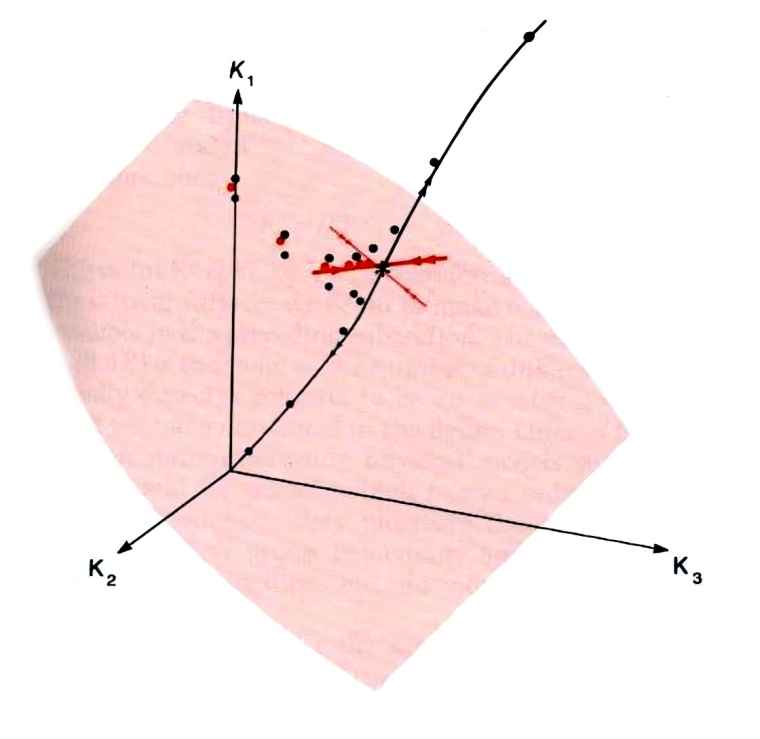
\includegraphics[width=0.8\linewidth,height=\textheight,keepaspectratio]{phase-transitions/Figs/flow2.png}

}

\caption{\label{fig-flow2}General flow in coupling space}

\end{figure}%

Figure~\ref{fig-flow2} is a representation of the space of all coupling
strengths \(K_a\) in the energy function \({\cal H}/k_BT\). This is of
course actually a space of infinite dimension, but representing three of
these, as we have done, enables us to illustrate all the important
aspects. First let us be clear what the points in this space represent.
Suppose we have some magnetic material which is described by a given set
of exchange constants \(J_1,J_2,J_3.....\) As the temperature \(T\)
varies, the coupling strengths \(K_a=J_a/k_BT\) trace out a straight
line, or ray, from the origin of the space in the direction
(\(J_1,J_2,J_3 ....\) ). Points on this ray close to the origin
represent this magnet at high temperatures, and conversely points far
from the origin represent the magnet at low temperatures. The critical
point of the magnet is represented by a specific point on this ray,
\(K_a=
J_a/k_BT, a= 1,2,\dots\) The set of critical points on all of the
possible rays forms a \emph{surface}, the critical surface. Formally, it
is defined by the set of all possible models (of the Ising type) which
have infinite \(\xi\). It is shown schematically as the shaded surface
in Figure~\ref{fig-flow2}. (In the figure it is a two-dimensional
surface; more generally it has one dimension less than the full coupling
constant space, dividing all models into high and low temperature
phases.)

Our immediate goal then is to understand how the RGT can explain why
different physical systems near this critical surface have the same
behaviour. Let us turn now to the schematic representation of the RG
flow in Figure~\ref{fig-flow2}. Suppose we start with a physical system,
with coupling strengths \(K_a,  a= 1,2, \dots\). What the RGT does is
generate a new point in the figure, at the coupling strengths
\(K_a^{(1)}=f_a({\bf K})\); these are the couplings appearing in the
effective energy function describing the coarse-grained system. If we
repeat the transformation, the new energy function has coupling
strengths \(K_a^{(2)}=f_a({\bf K})\). Thus repeated application of the
transformation generates a flow of points in the figure: \({\bf K\to
K^{(1)}\to\dots\to K^{(n)}}\) where the superscript (\(n\)) labels the
effective couplings after \(n\) coarse-graining steps. if the change in
coarse-graining scale is \(b\) (\(> 1\)) at each step, the total change
in coarse-graining scale is \(b^n\) after \(n\) steps. In the process,
therefore, the ratio of \(\xi\) to coarse-graining scale is reduced by a
factor of \(b^{-n}\). The dots in Figure~\ref{fig-flow2} identify three
lines of RG flow starting from three systems differing only in their
temperature. (The flow lines are schematic but display the essential
features revealed in detailed calculations.)

Consider first the red dots which start from the nearest neighbour Ising
model at its critical point. The ratio of \(\xi\) to coarse-graining
scale is reduced by a factor b at each step, but, since it starts
infinite, it remains infinite after any finite number of steps. In this
case we can in principle generate an unbounded number of dots,
\({\bf K^{(1)}, K^{(2)},\dots,K^{(n)}}\), all of which lie in the
critical surface. The simplest behaviour of such a sequence as \(n\)
increases is to tend to a limit, \(K^*\), say. In such a case

\[K^*_a=f_a(K^*)~~~~ a= 1,2 .....\]

This point \({\bf K^*} \equiv K_1^*, K_2^*, \dots\) is therefore a
\emph{fixed point} which lies in the critical surface.

By contrast, consider the same magnet as before, now at temperature
\(T\) just greater than \(T_c\), its couplings \(K_a\), will be close to
the first red dot (in fact they will be slightly smaller) and so will
the effective couplings \(K_a^{(1)},K_2^{(2)},\dots\) of the
corresponding coarse-grained systems. The new flow will therefore appear
initially to follow the red dots towards the same fixed point. However,
the flow must eventually move away from the fixed point because each
coarse-graining now produces a model further from criticality. The
resulting flow is represented schematically by one set of black dots.
The other set of black dots shows the expected flow starting from the
same magnet slightly below its critical temperature.

We are now in a position to understand both universality and scaling
within this framework. We will suppose that there exists a single fixed
point in the critical surface which sucks in all flows starting from a
point in that surface. Then any system at its critical point will
exhibit large-length scale physics (large-block spin behaviour)
described by the single set of fixed point coupling constants. The
uniqueness of this limiting set of coupling constants is the essence of
critical point universality. It is, of course, the algebraic counterpart
of the unique limiting spectrum of coarse-grained configurations,
discussed in Section~\ref{sec-unipics}. Similarly the scale-invariance
of the critical point configuration spectrum (viewed on large enough
length scales) is expressed in the invariance of the couplings under
iteration of the transformation (after a number of iterations large
enough to secure convergence to the fixed point).

To understand the behaviour of systems near but not precisely at
critically we must make a further assumption (again widely justified by
explicit studies). The flow line stemming from any such system will, we
have argued, be borne towards the fixed point before ultimately
deviating from it after a number of iterations large enough to expose
the system's noncritical character. We assume that (as indicated
schematically in the streams of red and blue lines in
Figure~\ref{fig-flow2} the deviations lie along a single line through
the fixed point, the direction followed along this line differing
according to the sign of the temperature deviation \(T-T_c\). Since any
two sets of coupling constants on the line (on the same side of the
fixed point) are related by a suitable coarse-graining operation, this
picture implies that the large-length-scale physics of all near-
critical systems differs only in the matter of a length scale. This is
the essence of near-critical point universality.

\end{tcolorbox}

\chapter{The renormalisation group: effective coupling
viewpoint}\label{the-renormalisation-group-effective-coupling-viewpoint}

Let us begin by returning to our fundamental Equation~\ref{eq-probs},
which we rewrite as

\[p = Z^{-1}e^{-{\cal H}}\] where \({\cal H}\equiv E/k_BT\).

The first step is then to imagine that we generate, by a computer
simulation procedure for example, a sequence of configurations with
relative probability \(\exp(-{\cal H})\). We next adopt some
coarse-graining procedure which produces from these original
configurations a set of coarse-grained configurations. We then ask the
question: what is the energy function \({\cal H}^\prime\) of the
coarse-grained variables which would produce these coarse-grained
configurations with the correct relative probability
\(\exp(-{\cal H}^\prime)\)? Clearly the form of \({\cal H}^\prime\)
depends on the form of \({\cal H}\) thus we can write symbolically

\[{\cal H}^\prime=R({\cal H})\]

The operation \(R\), which defines the coarse-grained configurational
energy in terms of the microscopic configurational energy function is
known as a renormalisation group transformation (RGT). What it does is
to replace a hard problem by a less hard problem. Specifically, suppose
that our system is near a critical point and that we wish to calculate
its large-distance properties. If we address this task by utilizing the
configurational energy and appealing to the basic machinery of
statistical mechanics set out in Equation~\ref{eq-probs} and
Equation~\ref{eq-partition}, the problem is hard. It is hard because the
system has fluctuations on all the (many) length scales intermediate
between the correlation length \(\xi\) and the minimum length scale
\(L_\textrm{min}\).

However, the task may instead be addressed by tackling the
coarse-grained system described by the energy \({\cal H}^\prime\). The
large-distance properties of this system are the same as the
large-distance properties of the physical system, since coarse-graining
operation preserves large-scale configurational structure. In this
representation the problem is a little easier: while the \(\xi\)
associated with \({\cal H}^\prime\) is the same as the \(\xi\)
associated with \({\cal H}\), the minimum length scale of
\({\cal H}^\prime\) is bigger than that of \({\cal H}\). Thus the
statistical mechanics of \({\cal H}^\prime\) poses a
not-quite-so-many-length-scale problem, a problem which is effectively a
little less critical and is thus a little easier to solve. The benefits
accruing from this procedure may be amplified by repeating it. Repeated
application of \(R\) will eventually result in a coarse- grained energy
function describing configurations in which the \(\xi\) is no bigger
than the minimum length scale. The associated system is far from
criticality and its properties may be reliably computed by any of a wide
variety of approximation schemes. These properties are the desired
large-distance properties of the physical system. As explicit reference
to fluctuations of a given scale is eliminated by coarse-graining, their
effects are carried forward implicitly in the parameters of the
coarse-grained energy.

In order to setup the framework for a simple illustrative example, let
is return to the lattice Ising model for which the energy function
depended only on the product of nearest neighbour spins. The coefficient
of this product in the energy is the exchange coupling, \(J\). In
principle, however, other kinds of interactions are also allowed; for
example, we may have a product of second neighbour spins with strength
\(J_2\) or, perhaps, a product of four spins (at sites forming a square
whose side is the lattice spacing), with strength \(J_3\). Such
interactions in a real magnet have their origin in the quantum mechanics
of the atoms and electrons and clearly depend upon the details of the
system. For generality therefore we will allow a family of exchange
couplings \(J_1\),\(J_2\),\(J_3,\dots\), or \(J_a, a =
1,2,\dots\) In reduced units, the equivalent coupling strengths are
\(K_a =J_a/k_BT\). Their values determine uniquely the energy for any
given configuration.

\begin{quote}
We note that it is not only useful to allow for arbitrary kinds of
interactions: if we wish to repeat the transformation several (indeed
many) times, it is also necessary because even if we start with only the
nearest neighbour coupling in \({\cal H}\) the transformation will in
general produce others in \({\cal H}^\prime\).
\end{quote}

Now consider the coarse-graining procedure. Let us suppose that this
procedure takes the form of a `majority rule' operation in which the new
spins are assigned values \(+1\) or \(-1\) according to the signs of the
magnetic moments of the blocks with which they are associated. The new
energy function \({\cal H}^\prime\) will be expressible in terms of some
new coupling strengths \(K^\prime\) describing the interactions amongst
the new spin variables (and thus, in effect, the interactions between
blocks of the original spin variables). The RGT simply states that these
new couplings depend on the old couplings: \(K_1^\prime\) is some
function \(f_1\) of all the original couplings, and generally

\begin{equation}\phantomsection\label{eq-rgt}{K^\prime_a=f_a(K_1,K_2,\dots) =f_a({\bf K}),~~~~ a= 1, 2,\dots
}\end{equation} where \textbf{K} is shorthand for the set
\(K_1, K_2,\dots\)

\section{A simple example}\label{a-simple-example-1}

This example illustrates how one can perform the RG transformation
Equation~\ref{eq-rgt} directly, without recourse to a `sequence of
typical configurations'. The calculation involves a very crude
approximation which has the advantage that it simplifies the subsequent
analysis.

\begin{figure}

\centering{

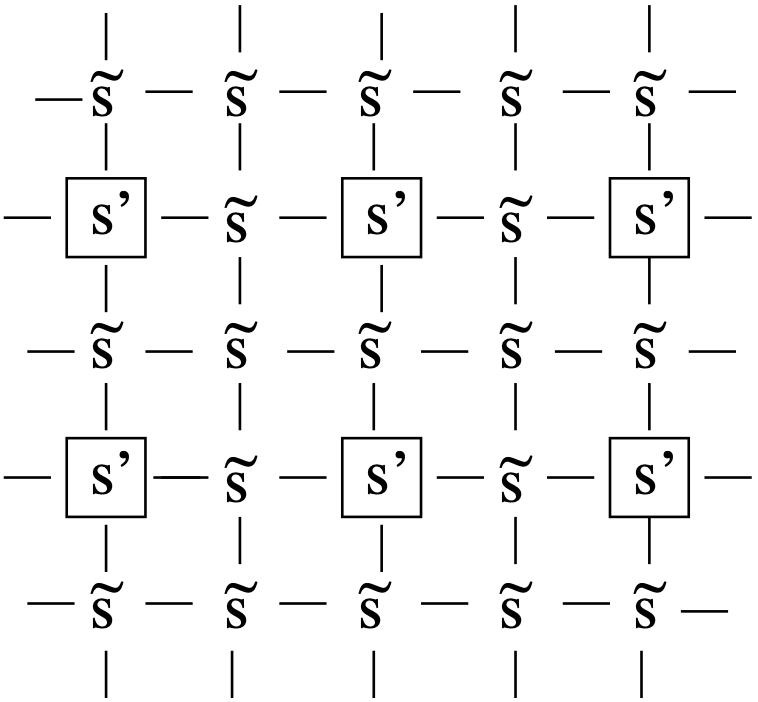
\includegraphics[width=0.4\linewidth,height=\textheight,keepaspectratio]{phase-transitions/Figs/rglat.png}

}

\caption{\label{fig-rglat}Coarse graining by decimation. The spins on
the original lattice are divided into two sets \(\{s^\prime\}\) and
\(\{\tilde{s}\}\). The \(\{s^\prime\}\) spins occupy a lattice whose
spacing is twice that of the original. The effective coupling
interaction between the \(\{s^\prime\}\) spins is obtained by performing
the configurational average over the \(\{\tilde{s}\}\)}

\end{figure}%

Consider an Ising model in two dimensions, with only nearest neighbour
interactions as shown in Figure~\ref{fig-rglat}. We have divided the
spins into two sets, the spins \(\{s^\prime\}\) form a square lattice of
spacing \(2\), the others being denoted by \(\{\tilde{s}\}\). One then
defines an effective energy function \({\cal H^\prime}\) for the
\(s^\prime\) spins by performing an average over all the possible
arrangements of the \(\tilde{s}\) spins

\begin{equation}\phantomsection\label{eq-decimate}{
\exp(-{\cal H}^\prime)=\sum_{\{\tilde {s}\}} \exp(-{\cal H}).
}\end{equation}

This particular coarse-graining scheme is called `decimation' because a
certain fraction (not necessarily one-tenth!) of spins on the lattice is
eliminated. This formulation of a new energy function realizes two basic
aims of the RG method: the long-distance physics of the `original'
system, described by \({\cal H}\), is contained in that of the `new'
system, described by \({\cal H}^\prime\) (indeed the partition functions
are the same as one can see by summing both sides over \(s^\prime\)) and
the new system is further from critically because the ratio of \(\xi\)
to lattice spacing (`minimum length scale') has been reduced by a factor
of \(1/2\) (the ratio of the lattice spacings of the two systems). We
must now face the question of how to perform the configuration sum in
Equation~\ref{eq-decimate}. This cannot in general be done exactly, so
we must resort to some approximation scheme. The particular
approximation which we invoke is the high temperature series expansion.
In its simplest mathematical form, since \({\cal H}\) contains a factor
\(1/k_BT\), it involves the expansion of \(\exp(-{\cal H})\) as a power
series:

\[\exp(-{\cal H}/k_BT)=1-{\cal H}/k_BT +\frac{1}{2!}({\cal H}/k_BT)^2+.....\]

We substitute this expansion into the right hand side of
Equation~\ref{eq-decimate} and proceed to look for terms which depend on
the \(s^\prime\) spins after the sum over the possible arrangements of
the \(\tilde{s}\) spins is performed. This sum extends over all the
possible (\(\pm 1\)) values of all the \(\tilde{s}\) spins. The first
term (the 1) in the expansion of the exponential is clearly independent
of the values of the \(s^\prime\) spins. The second term (\({\cal H}\))
is a function of the \(s^\prime\) spins, but gives zero when the sum
over the \(s^\prime\) spins is performed because only a single factor of
any \(s^\prime\) ever appears, and \(+ 1 - 1 = 0\). The third term
(\({\cal H}^2/2\)) does contribute. If one writes out explicitly the
form of \({\cal H}^2/2\) one finds terms of the form
\(K^2s_1^\prime\tilde{s}\tilde{s}s_2^\prime=K^2s_1^\prime s_2^\prime\),
where \(s_1^\prime\) and \(s_2^\prime\) denote two spins at nearest
neighbour sites on the lattice of \(s^\prime\) spins and \(\tilde{s}\)
is the spin (in the other set) which lies between them. Now, in the
corresponding expansion of the left hand side of
Equation~\ref{eq-decimate}, we find terms of the form
\(K^\prime s_1^\prime s_2^\prime\), where \(K^\prime\) is the nearest
neighbour coupling for the \(s^\prime\) spins. We conclude (with a
little more thought than we detail here) that

\begin{equation}\phantomsection\label{eq-rgdec}{
K^\prime=K^2
}\end{equation}

Of course many other terms and couplings are generated by the higher
orders of the high temperature expansion and it is necssary to include
these if one wishes reliable values for the critical temperature and
exponents, However, our aim here is to use this simple calculation to
illustrate the RG method. Let us therefore close our eyes, forget about
the higher order terms and show how the RGT Equation~\ref{eq-rgdec} can
be used to obtain information on the phase transition.

\begin{figure}

\centering{

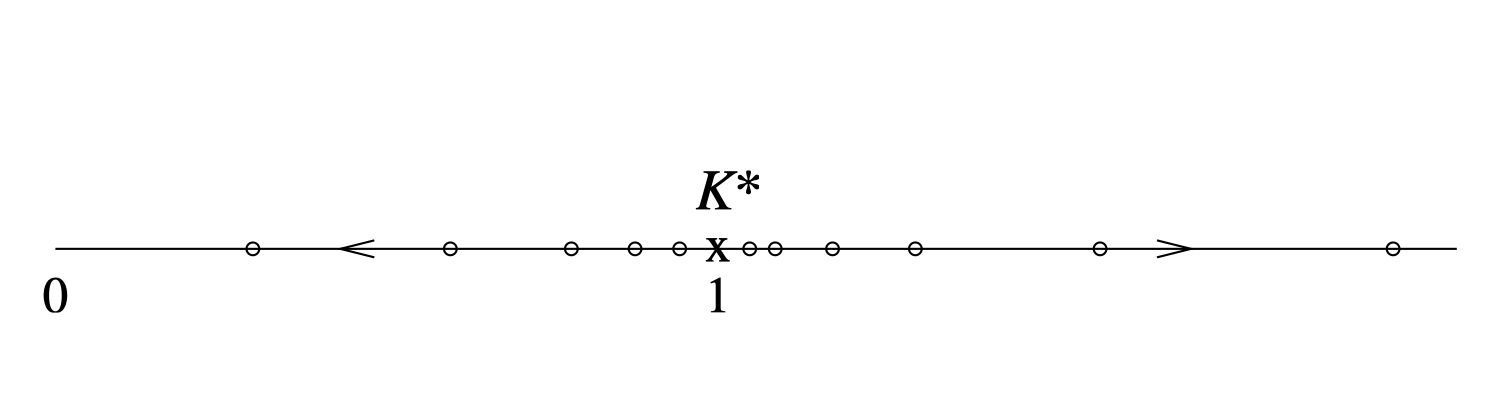
\includegraphics[width=0.6\linewidth,height=\textheight,keepaspectratio]{phase-transitions/Figs/flow1.png}

}

\caption{\label{fig-flow1}Coupling flow under the decimation
transformation described in the text.}

\end{figure}%

The first point to note is that that mathematically
Equation~\ref{eq-rgdec} has the fixed point \(K^*= 1\); if \(K= 1\) then
the new effective coupling \(K^\prime\) has the same value \(1\).
Further, if \(K\) is just larger than \(1\), then \(K^\prime\) is larger
than \(K\), i.e.~further away from \(1\). Similarly, if \(K\) is less
than \(1\), \(K^\prime\) is less than \(K\). We say that the fixed point
is unstable: the flow of couplings under repeated iteration of
Equation~\ref{eq-rgdec} is away from the fixed point, as illustrated in
Figure~\ref{fig-flow1}. The physical significance of this is as follows:
suppose that the original system is at its critical point so that the
ratio of \(\xi\) to lattice spacing is infinite. After one application
of the decimation transformation, the effective lattice spacing has
increased by a factor of two, but this ratio remains infinite; the new
system is therefore also at its critical point. Within the
approximations inherent in Equation~\ref{eq-rgdec}, the original system
is an Ising model with nearest neighbour coupling \(K\) and the new
system is an Ising model with nearest neighbour coupling \(K^\prime\).
If these two systems are going to be at a common critically, we must
identify \(K^\prime=
K\). The fixed point \(K^*= 1\) is therefore a candidate for the
critical point \(K_c\), where the phase transition occurs. This
interpretation is reinforced by considering the case where the original
system is close to, but not at, criticality. Then \(\xi\) is finite and
the new system is further from critically because the ratio of \(\xi\)
to lattice spacing is reduced by a factor of two. This instability of a
fixed point to deviations of \(K\) from \(K^*\) is a further necessary
condition for its interpretation as a critical point of the system. In
summary then we make the prediction

\begin{equation}\phantomsection\label{eq-Kc}{
K_c=J/k_BT_c=1
}\end{equation}

We can obtain further information about the behaviour of the system
close to its critical point. In order to do so, we rewrite the
transformation (Equation~\ref{eq-rgdec}) in terms of the deviation of
the coupling from its fixed point value. A Taylor expansion of the
function \(K^\prime=K^2\) yields \[
\begin{aligned}
K^\prime =& (K^*)^2 +(K-K^*)\left.\frac{\partial K^\prime}{\partial K}\right|_{K=K^*}+\frac{1}{2}(K-K^*)^2\left.\frac{\partial^2 K^\prime}{\partial K^2}\right|_{K=K^*}+\ldots\nonumber\\
K^\prime - K^* =& 2 (K - K^*)+ (K - K^*)^2 
\end{aligned}
\]

where in the second line we have used the fact that the first derivative
evaluates to \(2K^*=2\) and \((K^*)^2=K^*\).

For a system sufficiently close to its critical temperature the final
term can be neglected. The deviation of the coupling from its fixed
point (critical) value is thus bigger for the new system than it is for
the old by a factor of two. This means that the reduced temperature is
also bigger by a factor of two:

\[t^\prime= 2t\]

But \(\xi\) (in units of the appropriate lattice spacing) is smaller by
a factor of \(1/2\):

\[\xi^\prime= \xi/2\]

Thus, when we double \(t\), we halve \(\xi\), implying that

\[\xi\propto t^{-1}\]

for \(T\) close to \(T_c\). Thus we see that the RGT predicts scaling
behaviour with calculable critical exponents. In this simple calculation
we estimate the critical exponent \(\nu=1\) for the square lattice Ising
model. This prediction is actually in agreement with the exactly
established value. The agreement is fortuitous- the prediction in
Eq.~refeq:Kc for \(K_c\), is larger than the exactly established value
by a factor of more than two. In order to obtain reliable estimates more
sophisticated and systematic methods must be used.

The crude approximation in the calculation above produced a
transformation, Equation~\ref{eq-rgdec}, involving only the nearest
neighbour coupling, with the subsequent advantages of simple algebra. We
pay a penalty for this simplicity in two ways: the results obtained for
critical properties are in rather poor agreement with accepted values,
and we gain no insight into the origin of universality.

\section{Universality and scaling}\label{universality-and-scaling-2}

In order to expose how universality can arise, we should from the start
allow for several different kinds of coupling \(J_a\), and show how the
systems with \emph{different} \(J_a\) can have the \emph{same} critical
behaviour.

\begin{figure}

\centering{

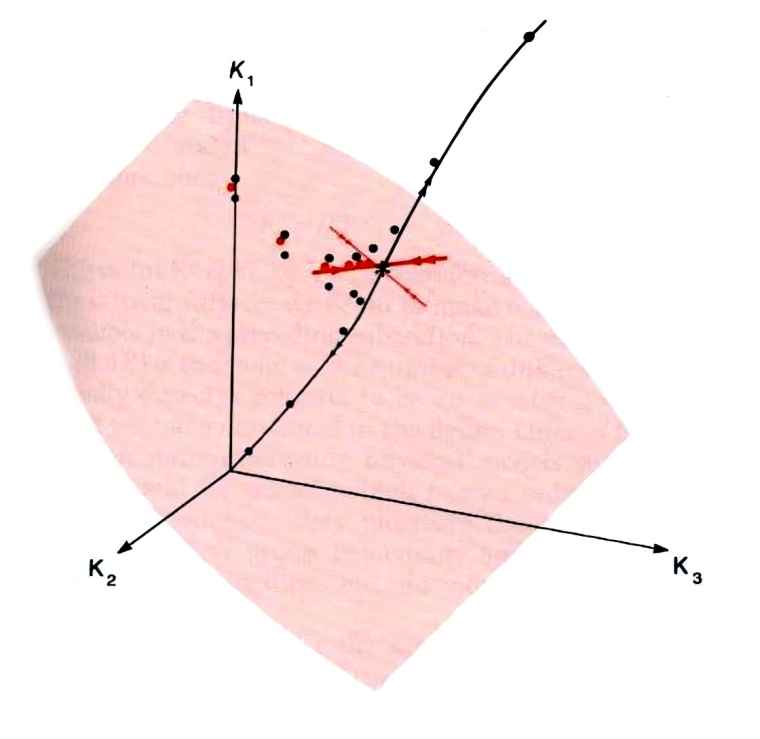
\includegraphics[width=0.8\linewidth,height=\textheight,keepaspectratio]{phase-transitions/Figs/flow2.png}

}

\caption{\label{fig-flow2}General flow in coupling space}

\end{figure}%

Figure~\ref{fig-flow2} is a representation of the space of all coupling
strengths \(K_a\) in the energy function \({\cal H}/k_BT\). This is of
course actually a space of infinite dimension, but representing three of
these, as we have done, enables us to illustrate all the important
aspects. First let us be clear what the points in this space represent.
Suppose we have some magnetic material which is described by a given set
of exchange constants \(J_1,J_2,J_3.....\) As the temperature \(T\)
varies, the coupling strengths \(K_a=J_a/k_BT\) trace out a straight
line, or ray, from the origin of the space in the direction
(\(J_1,J_2,J_3 ....\) ). Points on this ray close to the origin
represent this magnet at high temperatures, and conversely points far
from the origin represent the magnet at low temperatures. The critical
point of the magnet is represented by a specific point on this ray,
\(K_a=
J_a/k_BT, a= 1,2,\dots\) The set of critical points on all of the
possible rays forms a \emph{surface}, the critical surface. Formally, it
is defined by the set of all possible models (of the Ising type) which
have infinite \(\xi\). It is shown schematically as the shaded surface
in Figure~\ref{fig-flow2}. (In the figure it is a two-dimensional
surface; more generally it has one dimension less than the full coupling
constant space, dividing all models into high and low temperature
phases.)

Our immediate goal then is to understand how the RGT can explain why
different physical systems near this critical surface have the same
behaviour. Let us turn now to the schematic representation of the RG
flow in Figure~\ref{fig-flow2}. Suppose we start with a physical system,
with coupling strengths \(K_a,  a= 1,2, \dots\). What the RGT does is
generate a new point in the figure, at the coupling strengths
\(K_a^{(1)}=f_a({\bf K})\); these are the couplings appearing in the
effective energy function describing the coarse-grained system. If we
repeat the transformation, the new energy function has coupling
strengths \(K_a^{(2)}=f_a({\bf K})\). Thus repeated application of the
transformation generates a flow of points in the figure: \({\bf K\to
K^{(1)}\to\dots\to K^{(n)}}\) where the superscript (\(n\)) labels the
effective couplings after \(n\) coarse-graining steps. if the change in
coarse-graining scale is \(b\) (\(> 1\)) at each step, the total change
in coarse-graining scale is \(b^n\) after \(n\) steps. In the process,
therefore, the ratio of \(\xi\) to coarse-graining scale is reduced by a
factor of \(b^{-n}\). The dots in Figure~\ref{fig-flow2} identify three
lines of RG flow starting from three systems differing only in their
temperature. (The flow lines are schematic but display the essential
features revealed in detailed calculations.)

Consider first the red dots which start from the nearest neighbour Ising
model at its critical point. The ratio of \(\xi\) to coarse-graining
scale is reduced by a factor b at each step, but, since it starts
infinite, it remains infinite after any finite number of steps. In this
case we can in principle generate an unbounded number of dots,
\({\bf K^{(1)}, K^{(2)},\dots,K^{(n)}}\), all of which lie in the
critical surface. The simplest behaviour of such a sequence as \(n\)
increases is to tend to a limit, \(K^*\), say. In such a case

\[K^*_a=f_a(K^*)~~~~ a= 1,2 .....\]

This point \({\bf K^*} \equiv K_1^*, K_2^*, \dots\) is therefore a
\emph{fixed point} which lies in the critical surface.

By contrast, consider the same magnet as before, now at temperature
\(T\) just greater than \(T_c\), its couplings \(K_a\), will be close to
the first red dot (in fact they will be slightly smaller) and so will
the effective couplings \(K_a^{(1)},K_2^{(2)},\dots\) of the
corresponding coarse-grained systems. The new flow will therefore appear
initially to follow the red dots towards the same fixed point. However,
the flow must eventually move away from the fixed point because each
coarse-graining now produces a model further from criticality. The
resulting flow is represented schematically by one set of black dots.
The other set of black dots shows the expected flow starting from the
same magnet slightly below its critical temperature.

We are now in a position to understand both universality and scaling
within this framework. We will suppose that there exists a single fixed
point in the critical surface which sucks in all flows starting from a
point in that surface. Then any system at its critical point will
exhibit large-length scale physics (large-block spin behaviour)
described by the single set of fixed point coupling constants. The
uniqueness of this limiting set of coupling constants is the essence of
critical point universality. It is, of course, the algebraic counterpart
of the unique limiting spectrum of coarse-grained configurations,
discussed in Section~\ref{sec-unipics}. Similarly the scale-invariance
of the critical point configuration spectrum (viewed on large enough
length scales) is expressed in the invariance of the couplings under
iteration of the transformation (after a number of iterations large
enough to secure convergence to the fixed point).

To understand the behaviour of systems near but not precisely at
critically we must make a further assumption (again widely justified by
explicit studies). The flow line stemming from any such system will, we
have argued, be borne towards the fixed point before ultimately
deviating from it after a number of iterations large enough to expose
the system's noncritical character. We assume that (as indicated
schematically in the streams of red and blue lines in
Figure~\ref{fig-flow2} the deviations lie along a single line through
the fixed point, the direction followed along this line differing
according to the sign of the temperature deviation \(T-T_c\). Since any
two sets of coupling constants on the line (on the same side of the
fixed point) are related by a suitable coarse-graining operation, this
picture implies that the large-length-scale physics of all near-
critical systems differs only in the matter of a length scale. This is
the essence of near-critical point universality.

\chapter{Dynamics of first order phase transitions: nucleation, growth
and spinodal
decomposition}\label{dynamics-of-first-order-phase-transitions-nucleation-growth-and-spinodal-decomposition}

\section{Introduction to nucleation}\label{introduction-to-nucleation}

In previous discussions, we considered first-order phase transitions but
deferred a detailed analysis of the \emph{dynamical} mechanism by which
a system evolves from one phase to another. We now address this question
explicitly.

Consider again the Ising model at a temperature \(T < T_c\), where the
system is initially prepared in the majority spin-up phase at zero
external field, \(H = 0\). We now examine the system's response to the
application of a small negative external field \(H < 0\), which lowers
the free energy of the spin-down phase relative to the spin-up phase.

Despite the global free energy favoring the spin-down phase, the system
does not undergo an instantaneous transition. This delay is a
consequence of the free energy barrier associated with nucleating a
region of the stable phase within the metastable one, as introduced in
Section~\ref{sec-breaking}. The dynamical pathway of the phase
transition proceeds via \emph{nucleation} of localized
regions---referred to as \emph{droplets}---of the stable (spin-down)
phase embedded within the metastable (spin-up) background. Once
nucleated, these droplets may grow over time and ultimately coalesce to
transform the system to the stable phase.

The nucleation of a droplet of the stable phase of size \(n\) spins
entails a competition between bulk and interfacial contributions to the
free energy. The bulk free energy gain is linear in \(n\), given by
\(-nH\), due to the alignment of spins with the external field. However,
this gain is offset by an interfacial free energy cost arising from
broken bonds at the boundary between phases. For the Ising model, each
broken bond contributes an energy cost of \(+2J\), so the total
interfacial energy scales with the perimeter (in 2D) or surface area (in
3D) of the droplet. This interfacial contribution is referred to as the
\emph{surface tension}, and constitutes a true free energy cost: it
includes not only the energetic penalty from broken bonds but also an
entropic contribution due to the configurational degrees of freedom
associated with the droplet shape.

The resulting competition between the extensive free energy gain and the
sub-extensive interfacial cost leads to a free energy barrier for
droplet formation. Only fluctuations that produce a droplet larger than
a critical size \(n_c\) will grow; smaller droplets will shrink. This
framework is formalized in \emph{classical nucleation theory}, which
provides a quantitative description of the nucleation rate, critical
droplet size, and the associated activation energy barrier.

\section{Classical Nucleation Theory: Homogeneous
Nucleation}\label{sec-cnt}

We now present the framework of \textbf{classical nucleation theory}
(CNT) for the case of \emph{homogeneous nucleation}, in which the
nucleation of the stable phase occurs spontaneously and uniformly
throughout the bulk of the metastable phase, without the aid of
impurities, defects, or surfaces.

Let us consider a droplet of the stable (spin-down) phase of radius
\(R\) embedded within the metastable (spin-up) background. The total
change in free energy \(\Delta F(R)\) associated with forming such a
droplet consists of two competing contributions:

\begin{enumerate}
\def\labelenumi{\arabic{enumi}.}
\item
  \textbf{Bulk free energy gain}: The interior of the droplet consists
  of \(V \sim R^d\) spins aligned with the external field \(H < 0\),
  leading to a volume free energy change

  \[
  \Delta F_{\text{bulk}}(R) = -|\Delta f| \, R^d,
  \]

  where \(|\Delta f| \propto |H|\) is the free energy density difference
  between the metastable and stable phases, and \(d\) is the spatial
  dimensionality of the system.
\item
  \textbf{Interfacial free energy cost}: The boundary between the two
  phases has a surface area scaling as \(R^{d-1}\), and incurs a free
  energy cost proportional to the \emph{surface tension} \(\sigma\):

  \[
  \Delta F_{\text{surface}}(R) = \sigma \, S_d \, R^{d-1},
  \]

  where \(S_d\) is a geometrical factor (e.g., \(S_2 = 2\pi\) in 2D and
  \(S_3 = 4\pi\) in 3D).
\end{enumerate}

The total free energy change is therefore given by

\[
\Delta F(R) = \sigma \, S_d \, R^{d-1} - |\Delta f| \, V_d \, R^d,
\]

where \(V_d\) is another dimension-dependent constant. This expression
(Figure~\ref{fig-cnt-schem}) exhibits a characteristic maximum at a
critical droplet radius \(R_c\), obtained by extremizing \(\Delta F(R)\)
with respect to \(R\):

\[
\frac{d \Delta F}{dR} = 0 \quad \Rightarrow \quad R_c = \frac{(d-1)\sigma S_d}{d |\Delta f| V_d}.
\]

\begin{figure}

\centering{

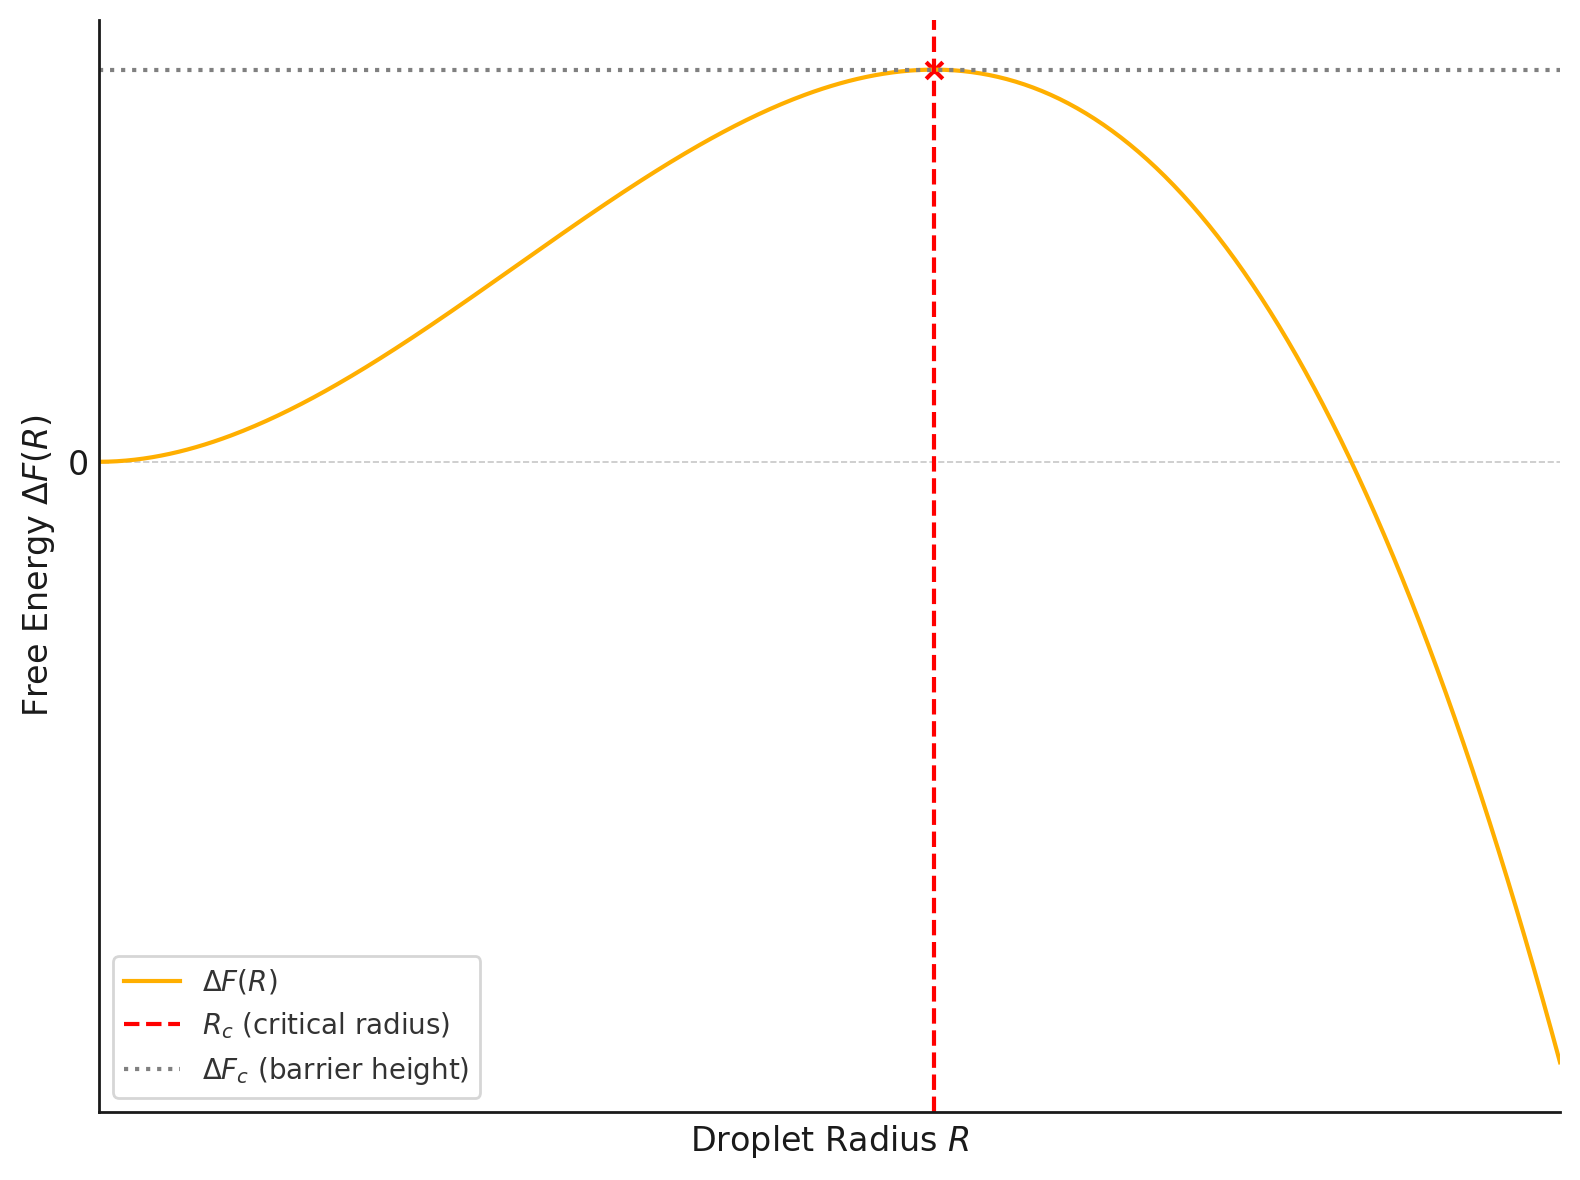
\includegraphics[width=0.5\linewidth,height=\textheight,keepaspectratio]{phase-transitions/Figs/cnt_schematic.png}

}

\caption{\label{fig-cnt-schem}Free energy barrier \(\Delta F(r)\) for
nucleation of a spherical droplet as a function of radius \(R\)
(schematic)}

\end{figure}%

The corresponding free energy barrier for nucleation is

\[
\Delta F_c = \Delta F(R_c) = \frac{(d-1)^{d-1}}{d^d} \cdot \frac{(S_d)^d \, \sigma^d}{(|\Delta f|)^{d-1} \, (V_d)^{d-1}}.
\]

This barrier must be surmounted by thermal fluctuations in order for a
critical nucleus to form and grow. The nucleation rate per unit volume
is given (in the Arrhenius approximation) by

\[
I \sim I_0 \exp\left( -\frac{\Delta F_c}{k_B T} \right),
\]

where \(I_0\) is a prefactor determined by microscopic kinetics, and
\(k_B\) is Boltzmann's constant.

\subsection{Interpretation and Scaling
Behavior}\label{interpretation-and-scaling-behavior}

Several key features emerge from this analysis:

\begin{itemize}
\tightlist
\item
  \textbf{Barrier scaling}: The nucleation barrier
  \(\Delta F_c \sim \sigma^d / |\Delta f|^{d-1}\) diverges as
  \(H \to 0\), reflecting the increasing stability of the metastable
  phase near the coexistence point.
\item
  \textbf{Critical radius}: The critical droplet size
  \(R_c \sim \sigma / |\Delta f|\) also diverges as
  \(|\Delta f| \to 0\), indicating that larger fluctuations are required
  to initiate nucleation close to the coexistence line.
\item
  \textbf{Dimensional dependence}: Both \(\Delta F_c\) and \(R_c\)
  exhibit strong dependence on the spatial dimension \(d\), with
  nucleation becoming increasingly suppressed in higher dimensions due
  to the dominance of interfacial cost.
\end{itemize}

In summary, homogeneous nucleation in a first-order transition is
governed by a delicate balance between surface tension and bulk free
energy gain. Only droplets exceeding a critical size can overcome the
barrier and initiate a transition. This sets an intrinsic timescale for
the dynamics of phase transformation, which can become extremely long
near coexistence due to the exponentially small nucleation rate.

\section{Domain growth}\label{domain-growth}

Following successful nucleation of a supercritical droplet, the system
enters a regime where the global transformation is driven by the
deterministic growth of domains of the stable phase. Such \emph{domain
growth} involves more atoms or molecules attaching to these nuclei,
causing them to expand into larger structures (e.g., growing crystals or
droplets).

Growth rate depends on factors like temperature, concentration, and the
availability of building blocks.

The shape and structure of the final phase often depend on how growth
occurs (e.g., slow growth may form perfect crystals; rapid growth may be
irregular).

\section{Spinodal decomposition}\label{spinodal-decomposition}

Previously we have considered a scenario in which we move our system to
a statepoint just inside the coexistence region so that the original
phase remains metastable. We then wait for a fluctuation that yields a
critical nucleus and subsequent growth.

Now imagine that rather than positioning the system just inside the
coexistence region we move immediately to a state point well inside the
coexistence region (cf. Figure~\ref{fig-spinodal}) such that there is no
metastable minimum in the free energy. Then there is no nucleation and
growth, rather the system is \emph{unstable} and immediately starts to
phase separate at all points in the system. This so called
\emph{spinodal decomposition}.

\begin{figure}

\centering{

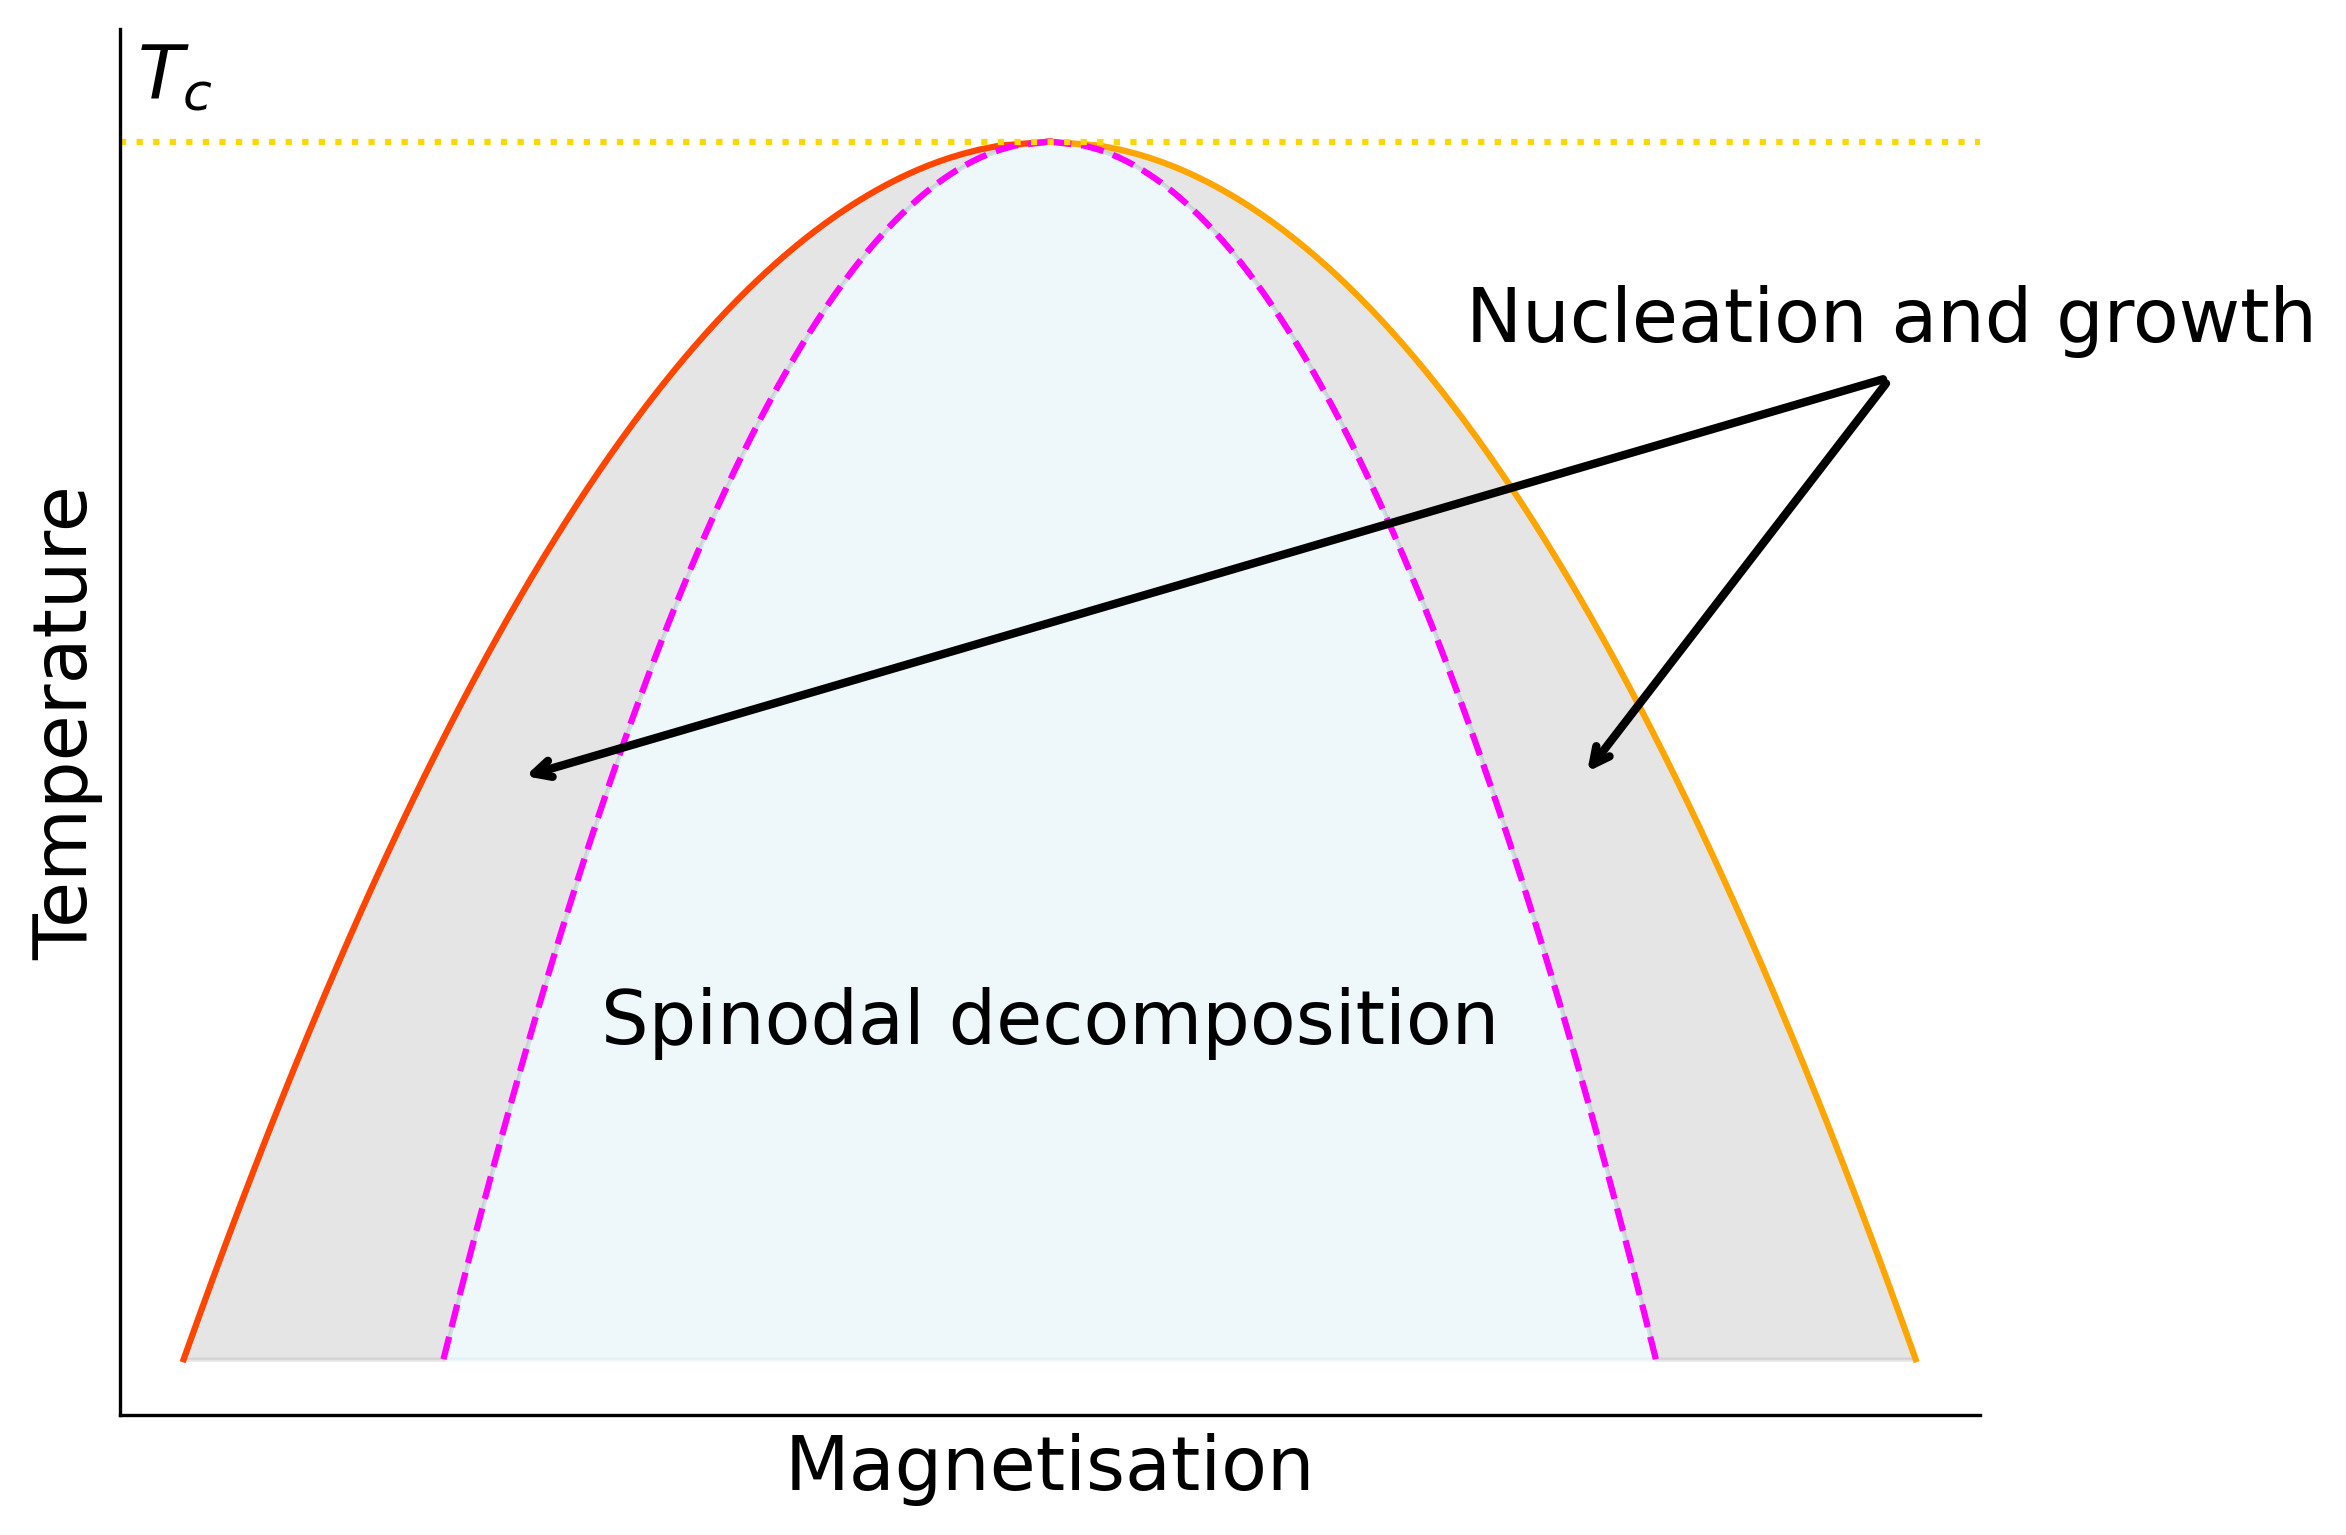
\includegraphics[width=0.5\linewidth,height=\textheight,keepaspectratio]{phase-transitions/Figs/spinodal.png}

}

\caption{\label{fig-spinodal}Schematic phase doagram showing the regions
in which one observes nucleation and growth, or spinodal decomposition}

\end{figure}%

The nature of spinodal decomposition and late-time domain growth depends
sensitively on whether the order parameter is conserved or not.

\begin{center}\rule{0.5\linewidth}{0.5pt}\end{center}

\subsection{Non-Conserved Order Parameter Dynamics (Model
A)}\label{non-conserved-order-parameter-dynamics-model-a}

In systems with a non-conserved order parameter, such as the Ising model
with single spin flip (so called Glauber) dynamics, the order parameter
can relax locally without constraint. This leads to curvature-driven
motion of interfaces.

The typical domain size \(L(t)\) grows algebraically with time:

\[
L(t) \sim t^{1/2},
\]

corresponding to a dynamic exponent \(z = 2\). The growth is driven by
reduction of the total interfacial area---regions of high curvature
(small domains) shrink and are absorbed by larger, flatter ones.

Let is aassume that domain walls move with velocity proportional to
curvature: \[
  v \sim \frac{1}{L}
  \] Then with the typical domain size being \(L(t)\) it follows that

\[
  \frac{dL}{dt} \sim \frac{1}{L}
  \]

Integrating both sides yields the \(t^{1/2}\) domain growth law.

It turns out that the detailed evolution of the coarse-grained order
parameter field \(\phi(\mathbf{r}, t)\) is governed by the
\textbf{Allen--Cahn equation}:

\[
\frac{\partial \phi}{\partial t} = - \frac{\delta F[\phi]}{\delta \phi},
\]

where \(F[\phi]\) is a coarse-grained Ginzburg--Landau free energy
functional:

\[
F[\phi] = \int d^d x \left[ \frac{1}{2} (\nabla \phi)^2 + V(\phi) \right],
\]

with \(V(\phi)\) typically a double-well potential such as
\(V(\phi) = \frac{1}{4}(\phi^2 - 1)^2\).

\begin{center}\rule{0.5\linewidth}{0.5pt}\end{center}

\subsection{Conserved Order Parameter Dynamics (Model
B)}\label{conserved-order-parameter-dynamics-model-b}

For systems with a conserved order parameter, such as phase separation
in binary alloys or the Ising model with spin-swap (so called
`Kawasaki') dynamics, the order parameter (e.g., composition or particle
number) must be conserved locally. This imposes a diffusive constraint
on the dynamics.

The domain size again grows algebraically, but with a different
exponent:

\[
L(t) \sim t^{1/3},
\]

corresponding to a dynamic exponent \(z = 3\).

A chemical potential difference drives diffusion and is given by \[
\Delta \mu \sim \frac{\sigma}{L}
\] (again due to curvature, where \(\sigma\) is surface tension)

Now the flux is proportional to the chemical potential gradient (Fick's
law): \[
\text{Flux} \sim -\nabla \mu \sim \frac{\Delta \mu}{L} \sim \frac{\sigma}{L^2}
\]

and the rate of change of domain size is proportional to this flux: \[
\frac{dL}{dt} \sim \frac{1}{L^2}
\quad\Rightarrow\quad
L(t) \sim t^{1/3}
\]

It turns out that the detailed dynamics are described by the
\textbf{Cahn--Hilliard equation}, a continuity equation of the form:

\[
\frac{\partial \phi}{\partial t} = \nabla^2 \left( \frac{\delta F[\phi]}{\delta \phi} \right),
\]

reflecting that the order parameter can only evolve via diffusion of its
conjugate chemical potential. This leads to the slow transport of
material across domains and a more sluggish coarsening process compared
to the non-conserved case.

\subsection{Schematic of Domain Growth in 2D Ising
model}\label{schematic-of-domain-growth-in-2d-ising-model}

Here are schematic illustrations of domain growth for:

\begin{itemize}
\item
  Non-conserved dynamics (Model A): Domains coarsen rapidly, with
  smoother and larger regions due to free relaxation of the order
  parameter.
\item
  Conserved dynamics (Model B): Coarsening is slower and domains are
  more intricate, reflecting the constraint of local conservation.
\end{itemize}

\begin{figure}

\begin{minipage}{0.50\linewidth}

\pandocbounded{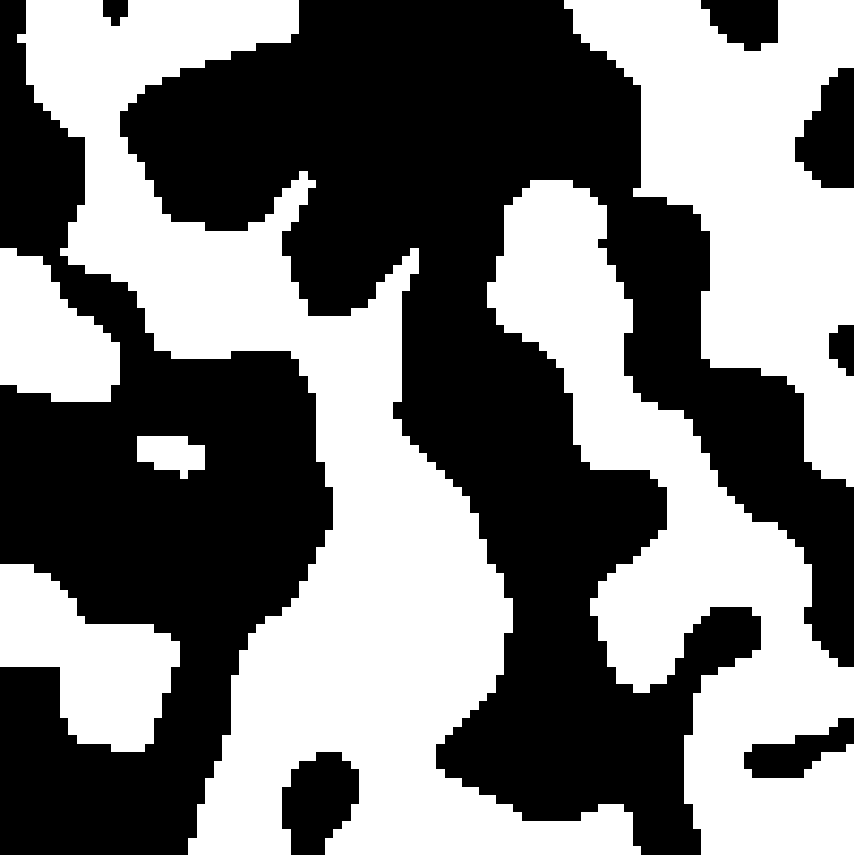
\includegraphics[keepaspectratio]{phase-transitions/Figs/non_conserved_domains.png}}

\subcaption{\label{}Non-Conserved Dynamics (Model A)}
\end{minipage}%
%
\begin{minipage}{0.50\linewidth}

\pandocbounded{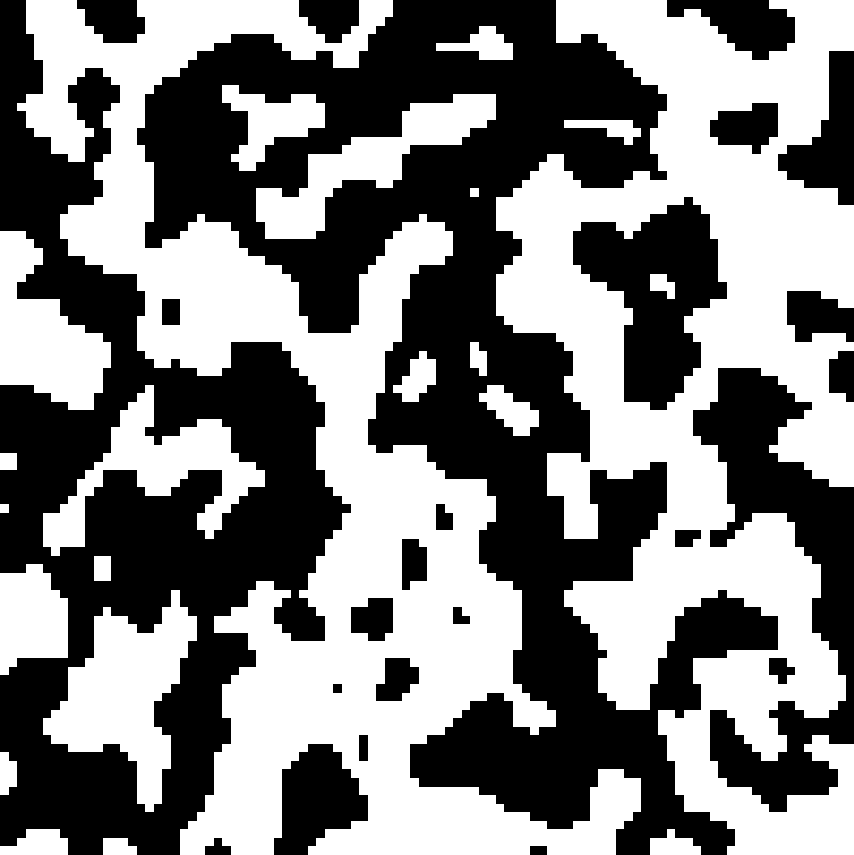
\includegraphics[keepaspectratio]{phase-transitions/Figs/conserved_domains.png}}

\subcaption{\label{}Conserved Dynamics (Model B)}
\end{minipage}%

\caption{\label{fig-growth}Schematic illustrations of domain morphology
resulting from spinodal decomposition or late-time domain growth for
non-conserved and conserved dynamics.}

\end{figure}%

\subsection{Dynamics Scaling
Hypothesis}\label{dynamics-scaling-hypothesis}

At late times, both conserved and non-conserved systems exhibit dynamic
scaling: the statistical properties of the domain morphology become
self-similar under rescaling of lengths by \(L(t)\).

For example, the equal-time two-point correlation function satisfies

\[
C(r, t) = f\left(\frac{r}{L(t)}\right),
\]

where \(f(x)\) is a time-independent scaling function. Plots of
\(C(r, t)\) collapse when plotted as a function of \(r/L(t)\).

The structure factor \(S(k, t)\), which is the Fourier transform of the
correlation function, is experimentally accessible eg via X-ray or
neutron scattering, and also obeys dynamic scaling:

\[
S(k, t) = \int d^d r \, e^{-i \vec{k} \cdot \vec{r}} \, C(r, t).
\]

Substituting the scaling form of \(C(r, t)\) into this expression, and
changing variables to \(\vec{u} = \vec{r}/L(t)\), gives:

\[
S(k, t) = L(t)^d \int d^d u \, e^{-i \vec{k} \cdot L(t) \vec{u}} \, f(u) = L(t)^d \, g(kL(t)),
\]

with \(g(x)\) a universal scaling function dependent on the dynamical
class and dimensionality.

\subsection{Summary of Growth Laws}\label{summary-of-growth-laws}

\begin{longtable}[]{@{}
  >{\raggedright\arraybackslash}p{(\linewidth - 8\tabcolsep) * \real{0.2523}}
  >{\raggedright\arraybackslash}p{(\linewidth - 8\tabcolsep) * \real{0.1308}}
  >{\raggedright\arraybackslash}p{(\linewidth - 8\tabcolsep) * \real{0.2243}}
  >{\raggedright\arraybackslash}p{(\linewidth - 8\tabcolsep) * \real{0.2243}}
  >{\raggedright\arraybackslash}p{(\linewidth - 8\tabcolsep) * \real{0.1682}}@{}}
\toprule\noalign{}
\begin{minipage}[b]{\linewidth}\raggedright
Dynamics Type
\end{minipage} & \begin{minipage}[b]{\linewidth}\raggedright
Conservation
\end{minipage} & \begin{minipage}[b]{\linewidth}\raggedright
Equation Type
\end{minipage} & \begin{minipage}[b]{\linewidth}\raggedright
Growth Law
\end{minipage} & \begin{minipage}[b]{\linewidth}\raggedright
Dynamic Exponent
\end{minipage} \\
\midrule\noalign{}
\endhead
\bottomrule\noalign{}
\endlastfoot
Model A (e.g.~Glauber) & No & Allen--Cahn & \(L(t) \sim t^{1/2}\) &
\(z = 2\) \\
Model B (e.g.~Kawasaki) & Yes & Cahn--Hilliard & \(L(t) \sim t^{1/3}\) &
\(z = 3\) \\
\end{longtable}

\begin{center}\rule{0.5\linewidth}{0.5pt}\end{center}

\begin{quote}
Remarks: The domain growth exponents \(1/z\) are robust under many
conditions, but can be modified in the presence of disorder, long-range
interactions, or hydrodynamic effects.
\end{quote}

\begin{quote}
In both the model A and model B cases, the system coarsens until it
reaches equilibrium, characterized by a uniform macroscopic phase and
the complete elimination of interfaces.
\end{quote}

\begin{quote}
The approach to equilibrium is algebraically slow (described by power
laws) due to the scale-free nature of domain dynamics.
\end{quote}

More about the scientists mentioned in this chapter:

\href{https://en.wikipedia.org/wiki/John_W._Cahn}{John Cahn}

\chapter{Introduction to stochastic
processes}\label{introduction-to-stochastic-processes}

Many natural phenomena are stochastic --- they involve randomness in
their evolution over time.

In classical physics, this randomness may arise from our lack of
knowledge about microscopic details. For example, in a gas, we do not
know the precise positions and velocities of each particle, so their
collisions with the container walls appear random.

In quantum mechanics, stochasticity is even more intrinsic. The
fundamental objects are probability amplitudes, and outcomes are
inherently probabilistic.

To describe these systems effectively, we use a coarse-grained
probabilistic description, which tracks the likelihood of different
outcomes rather than precise trajectories. One of the key tools in this
approach is the master equation.

\section{The Master Equation}\label{the-master-equation}

Consider a system in microstate \(i\) with energy \(E_i\). It can
transition to neighboring microstates \(j\), where the energy difference
\(|E_j - E_i|\) is small (within \(\delta E\)).

Let \(\nu_{ij}\) be the \textbf{rate} at which the system jumps from
state \(i\) to state \(j\). Over an infinitesimal time interval \(dt\),
the probability \(p_i\) changes as:

\[
dp_i = \left[ -p_i \sum_j  \nu_{ij} + \sum_j \nu_{ji} p_j \right] dt
\]

This expression contains two terms:

\begin{itemize}
\tightlist
\item
  A \emph{loss term}: the system leaves state \(i\) at rate
  \(\nu_{ij}\),
\item
  A \emph{gain term}: the system arrives in state \(i\) from other
  states \(j\) at rate \(\nu_{ji}\).
\end{itemize}

The master equation becomes:

\[
\frac{dp_i}{dt} = -\sum_j \nu_{ij} p_i + \sum_j \nu_{ji} p_j
\]

This is a linear first-order differential equation for the vector of
probabilities \(\{p_i\}\).

Alternatively, in matrix form:

\[
\frac{d\mathbf{p}}{dt} = W \mathbf{p}
\]

where \(W\) is the \textbf{rate matrix} with entries:

\begin{itemize}
\tightlist
\item
  \(W_{ij} = \nu_{ji}\) for \(i \neq j\),
\item
  \(W_{ii} = -\sum_{j \neq i} \nu_{ij}\).
\end{itemize}

This structure ensures probability conservation: the total probability
\(\sum_i p_i = 1\) remains constant in time.

The master equation is first order in time and does not have time
reversal symmetry so describes an irreversible process. This
irreversibility arises from the coarse-graining process that throws away
information about underlying microphysics which is described by Newton's
equations and which \emph{are} time reversible. Only by doing so is the
entropy allowed to increase which is required by the second law of
thermodynamics for an irreversible process. Consequently the increase of
entropy is linked to our knowledge about the system rather than anything
it is doing internally in a manner that may appear dubious. Can it be
possible that macroscopic and reproducible phenomena such as heat flow
depend on how we handle information? Perhaps yes since the division
between work and heat is somewhat arbitrary. Were we able to track all
the particle positions there would be no need to talk about heat energy
or heat flow.

\section{From the Master Equation to the Diffusion
Equation}\label{from-the-master-equation-to-the-diffusion-equation}

Now consider the situation where the state index \(i\) corresponds to a
position in space, \(x_i = i a\), ie a one-dimensional lattice with
lattice spacing \(a\), and transitions only occur between neighboring
lattice sites.

We assume:

\begin{itemize}
\item
  Transition rates are symmetric: \(\nu_{i, i+1} = \nu_{i, i-1} = \nu\),
\item
  The spacing \(a\to 0\) in the continuum limit.
\end{itemize}

The master equation becomes a finite-difference equation:

\[
\begin{aligned}
\frac{dp_i}{dt} =  &\sum_j\nu_{ij}(p_j-p_i)\\
\frac{dp_i}{dt} =  &\nu(p_{i-1}-p_i) + \nu(p_{i+1} - p_i)\\
\frac{dp_i}{dt} =  &\nu(p_{i+1} + p_{i-1} - 2p_i)
\end{aligned}
\]

We now define a continuous variable \(x = i a\), and a probability
density \(p(x, t)\) such that \(p_i(t) \approx p(x, t)\).

Using Taylor expansions:

\[
p(x \pm a, t) = p(x, t) \pm a \frac{\partial p}{\partial x} + \frac{a^2}{2} \frac{\partial^2 p}{\partial x^2} + \cdots
\]

Substituting into the master equation gives:

\[
\frac{\partial p}{\partial t} = 
\nu a^2 \frac{\partial^2 p}{\partial x^2}
\]

Defining the diffusion constant \(D = \nu a^2\), we obtain the
\textbf{diffusion equation}:

\[
\frac{\partial p}{\partial t} = D \frac{\partial^2 p}{\partial x^2}
\]

The diffusion equation describes the evolution of the probability
density of a particle with diffusion constant (sometimes called
diffusivity) given by \(D = \nu a^2\). The dimensions of \(D\) are
\([\text{length}]^2/[\text{time}]\). Typically, after expansion, we set
the lattice spacing \(a\) to 1. Additionally, the diffusion equation can
describe many non-interacting diffusing particles. In this case, we
replace \(p\) with \(\rho\), representing the density or concentration
of particles, and use the normalization \(\int dx \, \rho = M\), where
\(M\) is the number of particles.

The diffusion equation, much like the master equation from which it
originates, explicitly violates time-reversal symmetry, thus permitting
entropy to increase.

The solution of the diffusion equation for an initial condition where
the particle is initially localized at the origin (formally,
\(p(x,0) = \delta(x)\)) is a Gaussian:

\[
p(x,t) = (4 \pi D t)^{-1/2} \exp\left[-\frac{x^2}{4 D t}\right]
\]

We explicitly see the arrow of time by examining this Gaussian solution
at various times \(t\). As \(t\) increases, the Gaussian ``bell-shaped''
curve spreads out. Its width grows according to
\(\langle x^2 \rangle^{1/2} \sim t^{1/2}\). This is known as ``diffusive
scaling,'' and it implies that, after time \(t\), a particle will
typically be found at a distance roughly proportional to \(t^{1/2}\)
from its starting point. Conversely, exploring a region of size \(L\)
typically requires a time of order \(O(L^2)\).

The evolution of the solution to the 1d diffusion equation in a spatial
region \(x=[0,1]\) as a function of times are shown in the movie below.
The diffusion constant is \(D=0.01\). The movie corresponds to a
particle initialised at \(x=0.5\). One sees how the probability density
spreads out over the range as time increases. This can be used to model
the diffusion of particles down a concentration gradient as you will see
in the next part of the course.

\url{Movies/diffusion_evolution.mp4}

\begin{Shaded}
\begin{Highlighting}[]
\ImportTok{import}\NormalTok{ numpy }\ImportTok{as}\NormalTok{ np}
\ImportTok{import}\NormalTok{ matplotlib.pyplot }\ImportTok{as}\NormalTok{ plt}
\ImportTok{import}\NormalTok{ matplotlib.animation }\ImportTok{as}\NormalTok{ animation}
\ImportTok{import}\NormalTok{ os}

\CommentTok{\# Parameters}
\NormalTok{L }\OperatorTok{=} \FloatTok{1.0}        \CommentTok{\# Length of the domain}
\NormalTok{T }\OperatorTok{=} \FloatTok{1.0}        \CommentTok{\# Total time }
\NormalTok{nx }\OperatorTok{=} \DecValTok{400}       \CommentTok{\# Number of spatial points}
\NormalTok{nt }\OperatorTok{=} \DecValTok{2000}      \CommentTok{\# Number of time steps}
\NormalTok{D }\OperatorTok{=} \FloatTok{0.1}        \CommentTok{\# Diffusion coefficient}

\CommentTok{\# Discretization}
\NormalTok{dx }\OperatorTok{=}\NormalTok{ L }\OperatorTok{/}\NormalTok{ (nx }\OperatorTok{{-}} \DecValTok{1}\NormalTok{)}
\NormalTok{dt }\OperatorTok{=}\NormalTok{ T }\OperatorTok{/}\NormalTok{ nt}

\CommentTok{\# Stability condition auto{-}adjust}
\ControlFlowTok{if}\NormalTok{ D }\OperatorTok{*}\NormalTok{ dt }\OperatorTok{/}\NormalTok{ dx}\OperatorTok{**}\DecValTok{2} \OperatorTok{\textgreater{}} \FloatTok{0.5}\NormalTok{:}
    \BuiltInTok{print}\NormalTok{(}\StringTok{"Adjusting dt and nt to satisfy stability condition..."}\NormalTok{)}
\NormalTok{    dt }\OperatorTok{=} \FloatTok{0.4} \OperatorTok{*}\NormalTok{ dx}\OperatorTok{**}\DecValTok{2} \OperatorTok{/}\NormalTok{ D}
\NormalTok{    nt }\OperatorTok{=} \BuiltInTok{int}\NormalTok{(T }\OperatorTok{/}\NormalTok{ dt)}
\NormalTok{    dt }\OperatorTok{=}\NormalTok{ T }\OperatorTok{/}\NormalTok{ nt  }\CommentTok{\# Recalculate dt exactly}

\NormalTok{nt }\OperatorTok{=} \BuiltInTok{int}\NormalTok{(nt }\OperatorTok{/} \DecValTok{50}\NormalTok{)  }\CommentTok{\# Artificial slowdown for animation}

\BuiltInTok{print}\NormalTok{(}\SpecialStringTok{f"Using dt = }\SpecialCharTok{\{}\NormalTok{dt}\SpecialCharTok{:.4e\}}\SpecialStringTok{, nt = }\SpecialCharTok{\{}\NormalTok{nt}\SpecialCharTok{\}}\SpecialStringTok{"}\NormalTok{)}

\CommentTok{\# Initialize x and u}
\NormalTok{x }\OperatorTok{=}\NormalTok{ np.linspace(}\DecValTok{0}\NormalTok{, L, nx)}

\CommentTok{\# Initial condition: smooth narrow Gaussian}
\NormalTok{sigma }\OperatorTok{=} \FloatTok{0.01}
\NormalTok{u }\OperatorTok{=}\NormalTok{ np.exp(}\OperatorTok{{-}}\NormalTok{(x }\OperatorTok{{-}}\NormalTok{ L}\OperatorTok{/}\DecValTok{2}\NormalTok{)}\OperatorTok{**}\DecValTok{2} \OperatorTok{/}\NormalTok{ (}\DecValTok{2} \OperatorTok{*}\NormalTok{ sigma}\OperatorTok{**}\DecValTok{2}\NormalTok{))}

\CommentTok{\# Normalize initial condition}
\NormalTok{u }\OperatorTok{/=}\NormalTok{ np.}\BuiltInTok{sum}\NormalTok{(u) }\OperatorTok{*}\NormalTok{ dx}

\CommentTok{\# Setup figure}
\NormalTok{plt.rcParams.update(\{}
    \StringTok{"text.usetex"}\NormalTok{: }\VariableTok{True}\NormalTok{,}
    \StringTok{"font.family"}\NormalTok{: }\StringTok{"serif"}
\NormalTok{\})}

\NormalTok{fig, ax }\OperatorTok{=}\NormalTok{ plt.subplots()}
\NormalTok{line, }\OperatorTok{=}\NormalTok{ ax.plot(x, u)}

\CommentTok{\# Compute peak height for setting y{-}axis}
\NormalTok{peak\_height }\OperatorTok{=} \DecValTok{1} \OperatorTok{/}\NormalTok{ (np.sqrt(}\DecValTok{2} \OperatorTok{*}\NormalTok{ np.pi) }\OperatorTok{*}\NormalTok{ sigma)}
\NormalTok{ax.set\_ylim(}\DecValTok{0}\NormalTok{, peak\_height }\OperatorTok{*} \FloatTok{1.05}\NormalTok{)}

\NormalTok{ax.set\_xlabel(}\VerbatimStringTok{r\textquotesingle{}}\DecValTok{$}\VerbatimStringTok{x}\DecValTok{$}\VerbatimStringTok{\textquotesingle{}}\NormalTok{, fontsize}\OperatorTok{=}\DecValTok{20}\NormalTok{)}
\NormalTok{ax.set\_ylabel(}\VerbatimStringTok{r\textquotesingle{}}\DecValTok{$}\VerbatimStringTok{p}\KeywordTok{(}\VerbatimStringTok{x,t}\KeywordTok{)}\DecValTok{$}\VerbatimStringTok{\textquotesingle{}}\NormalTok{, fontsize}\OperatorTok{=}\DecValTok{20}\NormalTok{)}

\NormalTok{ax.tick\_params(axis}\OperatorTok{=}\StringTok{\textquotesingle{}both\textquotesingle{}}\NormalTok{, which}\OperatorTok{=}\StringTok{\textquotesingle{}major\textquotesingle{}}\NormalTok{, labelsize}\OperatorTok{=}\DecValTok{14}\NormalTok{)}

\CommentTok{\# Tiny time counter text}
\NormalTok{time\_text }\OperatorTok{=}\NormalTok{ ax.text(}\FloatTok{0.85}\NormalTok{, }\FloatTok{0.05}\NormalTok{, }\StringTok{\textquotesingle{}\textquotesingle{}}\NormalTok{, transform}\OperatorTok{=}\NormalTok{ax.transAxes, fontsize}\OperatorTok{=}\DecValTok{10}\NormalTok{, verticalalignment}\OperatorTok{=}\StringTok{\textquotesingle{}bottom\textquotesingle{}}\NormalTok{)}


\CommentTok{\# Function to update the plot}
\KeywordTok{def}\NormalTok{ update(frame):}
    \KeywordTok{global}\NormalTok{ u}
\NormalTok{    unew }\OperatorTok{=}\NormalTok{ np.copy(u)}
\NormalTok{    unew[}\DecValTok{1}\NormalTok{:}\OperatorTok{{-}}\DecValTok{1}\NormalTok{] }\OperatorTok{=}\NormalTok{ u[}\DecValTok{1}\NormalTok{:}\OperatorTok{{-}}\DecValTok{1}\NormalTok{] }\OperatorTok{+}\NormalTok{ D }\OperatorTok{*}\NormalTok{ dt }\OperatorTok{/}\NormalTok{ dx}\OperatorTok{**}\DecValTok{2} \OperatorTok{*}\NormalTok{ (u[}\DecValTok{2}\NormalTok{:] }\OperatorTok{{-}} \DecValTok{2}\OperatorTok{*}\NormalTok{u[}\DecValTok{1}\NormalTok{:}\OperatorTok{{-}}\DecValTok{1}\NormalTok{] }\OperatorTok{+}\NormalTok{ u[:}\OperatorTok{{-}}\DecValTok{2}\NormalTok{])}
\NormalTok{    u }\OperatorTok{=}\NormalTok{ unew}

    \CommentTok{\# Normalize at every step}
\NormalTok{    u }\OperatorTok{/=}\NormalTok{ np.}\BuiltInTok{sum}\NormalTok{(u) }\OperatorTok{*}\NormalTok{ dx}

\NormalTok{    line.set\_ydata(u)}
\NormalTok{    current\_time }\OperatorTok{=}\NormalTok{ frame }\OperatorTok{*}\NormalTok{ dt}
\NormalTok{    time\_text.set\_text(}\VerbatimStringTok{r\textquotesingle{}}\DecValTok{$}\VerbatimStringTok{t=\%}\DecValTok{.}\VerbatimStringTok{4f}\DecValTok{$}\VerbatimStringTok{\textquotesingle{}} \OperatorTok{\%}\NormalTok{ current\_time)}
    \ControlFlowTok{return}\NormalTok{ line, time\_text}

\NormalTok{ani }\OperatorTok{=}\NormalTok{ animation.FuncAnimation(fig, update, frames}\OperatorTok{=}\NormalTok{nt, interval}\OperatorTok{=}\DecValTok{100}\NormalTok{, blit}\OperatorTok{=}\VariableTok{True}\NormalTok{)}


\CommentTok{\# Save the animation as a movie}
\NormalTok{Writer }\OperatorTok{=}\NormalTok{ animation.writers[}\StringTok{\textquotesingle{}ffmpeg\textquotesingle{}}\NormalTok{]}
\NormalTok{writer }\OperatorTok{=}\NormalTok{ Writer(fps}\OperatorTok{=}\DecValTok{15}\NormalTok{, metadata}\OperatorTok{=}\BuiltInTok{dict}\NormalTok{(artist}\OperatorTok{=}\StringTok{\textquotesingle{}Me\textquotesingle{}}\NormalTok{), bitrate}\OperatorTok{=}\DecValTok{1800}\NormalTok{)}
\NormalTok{ani.save(}\StringTok{"../Movies/diffusion\_evolution.mp4"}\NormalTok{, writer}\OperatorTok{=}\NormalTok{writer)}


\NormalTok{plt.show()}
\end{Highlighting}
\end{Shaded}

\section{Consequences of time reversal
symmetry}\label{consequences-of-time-reversal-symmetry}

As we have seen by introducing a type of coarse graining, the master
equation violates time reversal symmetry of the underlying Newtonian
dynamics. Remarkably however, the fact that the underlying microphysics
is actually time reversal symmetric has several deep consequences which
survive the coarse graining procedure These results are some of the
cornerstones of nonequilibrium thermodynamics

\subsection{Detailed balance}\label{detailed-balance}

Recall from year 2 Statistical Mechanics that for a system in
equilibrium, the principle of equal a-priori probabilities of
microstates holds. Therefore

\[
\nu_{ij} p_i^{eq} = \nu_{ji} p_j^{eq}
\]

Hence, on average, the actual rate of quantum jumps from \(i\) to \(j\)
(the left-hand side) is the same as from \(j\) to \(i\). This is a
stronger statement than the master equation, which asserts only that
there is overall balance between the rate of jumping into and out of
state \(i\) in equilibrium. The result above is known as the
\emph{principle of detailed balance}.

This principle is powerful because it applies not only to individual
states but also to any grouping of states.

\emph{Exercise:} Show that for two groups of states, \(A\) and \(B\),
the overall rate of transitions from group \(A\) to group \(B\) is
balanced, in equilibrium, by those from \(B\) to \(A\):

\[
\nu_{AB} p_A^{eq} = \nu_{BA} p_B^{eq}
\]

Hence, detailed balance arguments can be extended to subsystems within a
large isolated system, and even to systems that are not isolated.
However, in such cases, the principle is far from obvious, because once
states are grouped together:

\[
\nu_{AB} \ne \nu_{BA}, \quad p_A \ne p_B
\]

(This can be easily demonstrated, for example, by considering two groups
that contain different numbers of states with similar energies.)
Nonetheless, the detailed balance relation holds, in equilibrium, in the
general form above.

\subsection{Computer simulation}\label{computer-simulation}

In computer simulation, good results will be obtained if one accurately
follows the microscopic equations of motion. This is the \emph{molecular
dynamics (MD)} method which we now outline.

\textbf{Molecular dynamics}

Molecular Dynamics (MD) involves a system of classical particles
interacting through specified interparticle forces. The motion of these
particles is determined by numerically integrating Newton's equations of
motion. In MD simulations, averages of state variables are obtained as
time averages over trajectories in phase space. Typically, the forces
acting between particles are conservative, ensuring that the total
energy \(E\) remains constant. This conservation implies that the motion
is restricted to a \((2dN - 1)\)-dimensional surface in phase space,
denoted by \(\Gamma(E)\).

A central aspect of MD is the averaging of observables. For a given
observable \(A\), its average is computed as the time average along the
trajectory. Mathematically, this is expressed as:

\[
\left\langle A(\{ \mathbf{p}_i \}, \{ \mathbf{r}_i \}) \right\rangle = \frac{1}{\tau} \int_{t_0}^{t_0+\tau} dt\, A(\{ \mathbf{p}_i(t) \}, \{ \mathbf{r}_i(t) \})
\]

This formula represents the integral of the observable over a time
interval \(\tau\), normalized by the length of that interval.

The practical steps of an MD simulation start with generating an initial
random configuration of particle positions \(\{ \mathbf{r}_i \}\) and
momenta \(\{ \mathbf{p}_i \}\). The system's equations of motion are
then iteratively solved using a suitable algorithm to allow it to reach
equilibrium. After equilibration, a production run is performed over
many time steps to collect meaningful data. Finally, relevant averages,
such as pressure or kinetic energy, are calculated from the collected
data.

\textbf{Monte Carlo}

However, to obtain the equilibrium properties of the system, it may be
much faster to use a dynamics which is nothing like the actual equations
of motion.

At first sight, this looks very dangerous; however, if one can prove
that in the required equilibrium distribution, the artificial dynamics
obey the principle of detailed balance, then it is (almost) guaranteed
that the steady state found by simulation is the true equilibrium state.

The best known example is the \emph{Monte Carlo method}, in which the
dynamical algorithm consists of random jumps. The jump rates
\(\nu_{AB}\) for all pairs of states \((A, B)\) take the form:

\[
\nu_{AB} = \nu_0 \quad \text{if } E_B \le E_A
\]

\[
\nu_{AB} = \nu_0 e^{-\beta (E_B - E_A)} \quad \text{if } E_B \ge E_A
\]

where \(\nu_0\) is a constant.

\emph{Exercise:} Show that this gives the canonical distribution in
steady state.

\begin{tcolorbox}[enhanced jigsaw, toprule=.15mm, opacityback=0, colbacktitle=quarto-callout-caution-color!10!white, title=\textcolor{quarto-callout-caution-color}{\faFire}\hspace{0.5em}{Solution}, leftrule=.75mm, rightrule=.15mm, bottomtitle=1mm, breakable, colframe=quarto-callout-caution-color-frame, colback=white, toptitle=1mm, left=2mm, titlerule=0mm, coltitle=black, arc=.35mm, bottomrule=.15mm, opacitybacktitle=0.6]

To show that this jump rate rule gives the canonical distribution in
steady state, we assume the system reaches a steady-state probability
distribution \(P_A\) for state \(A\) and apply the condition of detailed
balance.

Detailed balance requires: \[
P_A \nu_{AB} = P_B \nu_{BA}
\]

Assume the canonical distribution: \[
P_A = \frac{1}{Z} e^{-\beta E_A}, \quad P_B = \frac{1}{Z} e^{-\beta E_B}
\]

Now consider two cases for \(\nu_{AB}\) and \(\nu_{BA}\):

\textbf{Case 1:} \(E_B \leq E_A\)

Then: \[
\nu_{AB} = \nu_0, \quad \nu_{BA} = \nu_0 e^{-\beta (E_A - E_B)}
\]

Substitute into the detailed balance condition: \[
P_A \nu_0 = P_B \nu_0 e^{-\beta (E_A - E_B)}
\]

Cancel \(\nu_0\): \[
P_A = P_B e^{-\beta (E_A - E_B)}
\]

Use canonical form: \[
\frac{1}{Z} e^{-\beta E_A} = \frac{1}{Z} e^{-\beta E_B} e^{-\beta (E_A - E_B)} = \frac{1}{Z} e^{-\beta E_A}
\]

Verified.

\textbf{Case 2:} \(E_B > E_A\)

Then: \[
\nu_{AB} = \nu_0 e^{-\beta (E_B - E_A)}, \quad \nu_{BA} = \nu_0
\]

Substitute: \[
P_A \nu_0 e^{-\beta (E_B - E_A)} = P_B \nu_0
\]

Cancel \(\nu_0\): \[
P_A e^{-\beta (E_B - E_A)} = P_B
\]

Again using canonical form: \[
\frac{1}{Z} e^{-\beta E_A} e^{-\beta (E_B - E_A)} = \frac{1}{Z} e^{-\beta E_B} = P_B
\]

Verified.

Hence, in both cases the detailed balance condition is satisfied with
the canonical distribution, and the steady state is indeed the canonical
distribution.

\end{tcolorbox}

\chapter{The Langevin Approach}\label{the-langevin-approach}

\section{The Random Walk and the Langevin
equation}\label{the-random-walk-and-the-langevin-equation}

The concept of a random walk and its continuum limit -- diffusion --
introduced in the previous chapter, expresses the time evolution of the
probability distribution \(p(x, t)\) for a particle's position \(x\) by
the diffusion equation:

\[
\frac{\partial p}{\partial t} = D \frac{\partial^2 p}{\partial x^2},
\]

which is a standard example of a so called \emph{Fokker-Planck}
equation, which is second-order in space and first-order in time.

In contrast, the \emph{Langevin equation} provides a stochastic
differential equation for the particle's trajectory \(x(t)\). To
understand it, consider the random hopping motion of a particle on a 1d
lattice over a small time increment \(\Delta t\):

\[
x(t + \Delta t) = x(t) + \Delta x(t)
\]

Here, \(\Delta x(t)\) is a random displacement. If the lattice spacing
is \(a\), we define the step statistics as:

\[
\Delta x(t) = 
\begin{cases}
+a & \text{with probability } \nu \Delta t \\
-a & \text{with probability } \nu \Delta t \\
0 & \text{with probability } 1 - 2\nu \Delta t
\end{cases}
\]

This defines a discrete-time, discrete-space random walk. The average
and variance of the step are easily derived using binomial statistics:

\begin{itemize}
\item
  Mean: \(\langle \Delta x \rangle = 0\)
\item
  Variance:
  \(\langle (\Delta x)^2 \rangle = 2 a^2 \nu \Delta t = 2D \Delta t\)
\end{itemize}

The steps \(\Delta x(t)\) are uncorrelated across time.

To take the continuum limit, we let both \(a \to 0\) and
\(\Delta t \to 0\) in such a way that:

\[
a \propto \sqrt{\Delta t}
\]

In this limit, we obtain the \textbf{Langevin equation}:

\[
\dot{x}(t) = \eta(t)
\]

where \(\eta(t)\equiv\frac{\Delta x(t)}{\Delta t}\) is a stochastic
noise satisfying:

\[
\langle \eta(t) \rangle = 0
\]

\[
\langle \eta(t) \eta(t') \rangle = \Gamma \delta(t - t')
\]

This \(\eta(t)\) is known as white noise --- it has zero mean and is
uncorrelated at different times. \(\Gamma\) measures its amplitude.

The Langevin equation tells us that the velocity \(\dot{x}(t)\) is
purely driven by noise. We can formally integrate it:

\[
x(t) - x_0 = \int_0^t \eta(t')\, dt'
\]

Taking ensemble averages:

\begin{itemize}
\item
  Mean displacement: \[
  \langle x(t) - x_0 \rangle = 0
  \]
\item
  Mean square displacement: \[
  \langle [x(t) - x_0]^2 \rangle = \int_0^t \int_0^t \langle \eta(t') \eta(t'') \rangle\, dt'\, dt'' = \Gamma \int_0^t dt' = \Gamma t
  \]
\end{itemize}

Comparing this with the diffusion equation result, we identify:

\[
\Gamma = 2D
\]

Hence, the Langevin description yields the same physical behavior ---
not just the mean-square displacement but also the full probability
distribution \(p(x, t)\) --- as the diffusion (Fokker-Planck) equation.
This equivalence arises from the fact that the integral of many small,
independent random steps leads to a Gaussian distribution, in agreement
with the solution of the diffusion equation.

For more details, see: \emph{Stochastic Processes in Physics and
Chemistry} by N.G. van Kampen (North Holland, 1981).

\section{Brownian Motion}\label{brownian-motion}

Let us now examine Brownian motion, originally observed as the erratic
motion of colloidal particles suspended in a fluid. These particles
undergo constant collisions with surrounding (smaller) fluid molecules,
which results in seemingly random movement.

From a coarse-grained perspective --- where we do not track each
individual collision --- this appears as motion under random forces.
This statistical treatment introduces irreversibility at the macroscopic
level, even though the underlying molecular dynamics are reversible.

The Langevin equation provides a way to model this behavior. For a
particle of mass \(m\) in one dimension, Langevin proposed the equation:

\[
m \ddot{x} = -\gamma \dot{x} + f(t)
\]

Here:

\begin{itemize}
\tightlist
\item
  \(-\gamma \dot{x}\) is a frictional damping force, where \(\gamma\) is
  the damping coefficient.
\item
  \(f(t)\) is a random force due to molecular collisions.
\end{itemize}

\begin{quote}
Often, the mobility is defined as \(\mu = 1/\gamma\) --- note that this
is unrelated to chemical potential.
\end{quote}

\subsection{Noise Properties}\label{noise-properties}

In principle the random forces are correlated in time since the
molecular collisions which cause them are correlated and have some
definite duration.

Let us assume that there is some correlation time \(t_c\) over which
\(\langle f(t_1) f(t_2) \rangle = g(t_1 - t_2)\) decays rapidly as shown
in the sketch below:

\begin{figure}

\centering{

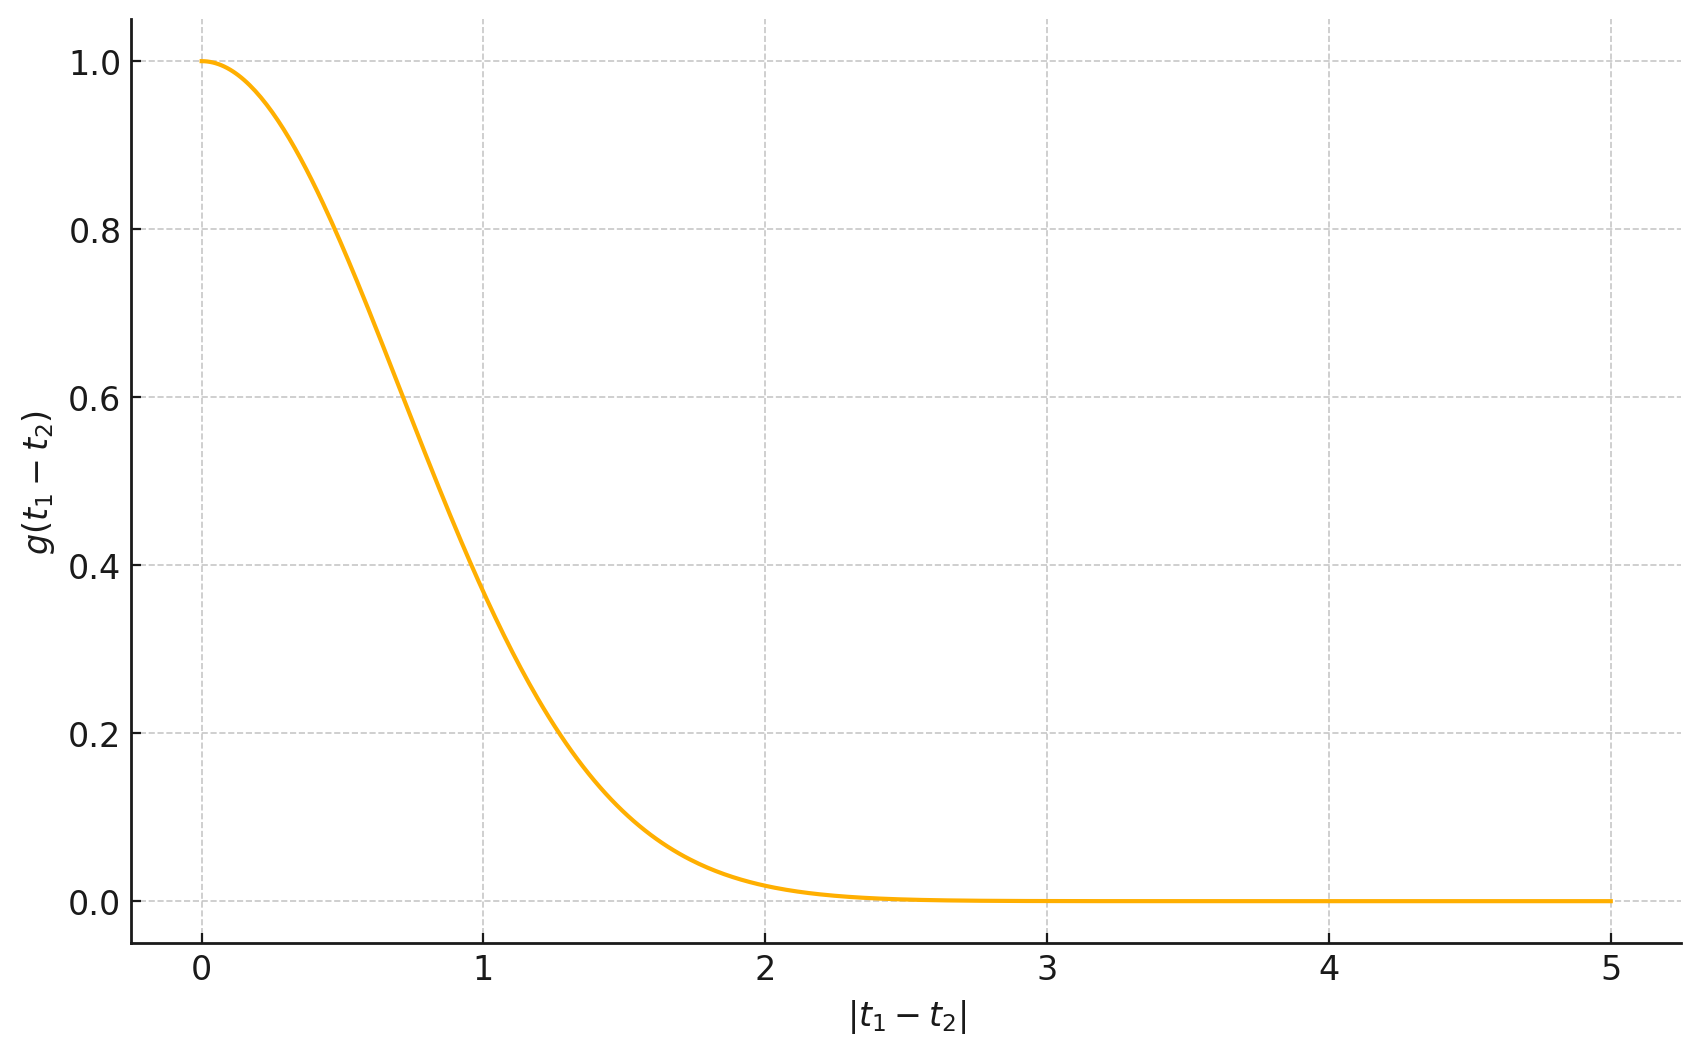
\includegraphics[width=0.6\linewidth,height=\textheight,keepaspectratio]{phase-transitions/Figs/autocorrelate.png}

}

\caption{\label{fig-autocorrelate}Sketch of \(g(t1−t2)\) against
\(|t1− t2|\)}

\end{figure}%

Then as long as we consider timescales \(\gg t_c\) we can safely replace
\(g(t_1 - t_2)\) by a delta function. Thus we can make the approximation
of white noise

\[
\langle f(t) \rangle = 0
\]

\[
\langle f(t_1) f(t_2) \rangle = \Gamma \delta(t_1 - t_2)
\]

\subsection{Solving the Langevin Equation
(velocity)}\label{solving-the-langevin-equation-velocity}

Let's set \(m = 1\) for simplicity and solve the equation:

\[
\dot{v} + \gamma v = f(t)
\]

We apply an integrating factor:

\[
\frac{d}{dt} \left[ v e^{\gamma t} \right] = e^{\gamma t} f(t)
\]

Integrating both sides:

\[
v(t) = v_0 e^{-\gamma t} + \int_0^t e^{-\gamma (t - t')} f(t')\, dt'
\]

Taking the average:

\[
\langle v(t) \rangle = v_0 e^{-\gamma t}
\]

Thus:

\begin{itemize}
\tightlist
\item
  At short times: (\(\gamma t \ll 1\)):
  \(\langle v \rangle \approx v_0\) ie. friction is negligible.
\item
  At long times: (\(\gamma t \gg 1\)): \(\langle v \rangle \to 0\) ie.
  the system loses memory of the initial velocity.
\end{itemize}

\subsection{Mean-square velocity}\label{mean-square-velocity}

We now compute:

\[
\langle v(t)^2 \rangle = v_0^2 e^{-2\gamma t} + \Gamma \int_0^t e^{-2\gamma (t - t')} dt' = v_0^2 e^{-2\gamma t} + \frac{\Gamma}{2\gamma} \left(1 - e^{-2\gamma t} \right)
\]

Implying that at

\begin{itemize}
\tightlist
\item
  Short times: \(\langle v^2 \rangle \approx v_0^2\)
\item
  Long times: \(\langle v^2 \rangle \to \Gamma / (2\gamma)\)
\end{itemize}

At equilibrium, the equipartition theorem gives:

\[
\frac{1}{2} m \langle v^2 \rangle = \frac{1}{2} k_B T
\]

Using this to identify \(\Gamma\):

\[
\Gamma = 2 \gamma k_B T
\]

This important result relates the noise strength to the damping and
temperature --- they have the same microscopic origin (molecular
collisions).

\subsection{Mean-square displacement}\label{mean-square-displacement}

We now integrate \(v(t)\) again to get position \(x(t)\) (with
\(m = 1\)):

Using the result above and substituting \(\Gamma = 2\gamma k_B T\), we
find:

\[
\langle [x(t) - x_0]^2 \rangle = \frac{(v_0^2 - k_B T)}{\gamma^2} (1 - e^{-\gamma t})^2 + \frac{2 k_B T}{\gamma} \left[ t - \frac{1 - e^{-\gamma t}}{\gamma} \right]
\]

Limiting behaviours:

\begin{itemize}
\item
  Short times: (\(\gamma t \ll 1\)):

  \[
  \langle [x(t) - x_0]^2 \rangle \approx v_0^2 t^2
  \]

  (correspinding to \emph{ballistic} motion)
\item
  Long time (\(\gamma t \gg 1\)):

  \[
  \langle [x(t) - x_0]^2 \rangle \approx \frac{2 k_B T}{\gamma} t
  \]

  (corresponding to \emph{diffusive motion})
\end{itemize}

\begin{figure}

\centering{

\includegraphics[width=0.6\linewidth,height=\textheight,keepaspectratio]{phase-transitions/Figs/brownian_crossover.png}

}

\caption{\label{fig-browniancross}Schematic plot of the crossover from
ballistic to diffusive motion for a colloid in a fluid.}

\end{figure}%

The effective diffusion constant is:

\[
D = \frac{k_B T}{\gamma}
\]

This is the \textbf{Einstein relation}, connecting the rate of diffusion
to temperature and damping. It is useful as it allows an explicit
expression for the diffusion constant if one knows \(\gamma\). A famous
example is a sphere: the equation for fluid flow past a moving sphere
may be solved and yields \(\gamma=6\pi\eta a\) where \(a\) is the radius
of the sphere and here \(\eta\) is the fluid viscosity. This gives

\[
D=\frac{6\pi\eta a}{kT}
\] which is the \textbf{Stokes-Einstein} formula for the diffusion
constant of a colloidal particle.

\subsection{External Forces and
Mobility}\label{external-forces-and-mobility}

Now consider a charged particle with charge \(q\) under an external
electric field \(E\). The Langevin equation becomes:

\[
m \dot{v} = -\gamma v + qE
\]

At long times, the particle reaches a steady drift velocity:

\[
\langle v \rangle = \frac{qE}{\gamma} = \frac{qED}{k_B T}
\]

Defining the mobility \(\mu\) by \(\langle v \rangle = \mu qE\), we get
the \textbf{Nernst-Einstein relation}:

\[
\mu = \frac{D}{k_B T}
\]

This relation connects the response of a system to an external
perturbation (mobility) with its internal fluctuations (diffusivity).

\subsection{Molecular Dynamics simulation of Brownian motion for a
colloid particle in a liquid
suspension}\label{molecular-dynamics-simulation-of-brownian-motion-for-a-colloid-particle-in-a-liquid-suspension}

\url{Movies/brownian_colloid.mp4}

\begin{Shaded}
\begin{Highlighting}[]
\ImportTok{import}\NormalTok{ numpy }\ImportTok{as}\NormalTok{ np}
\ImportTok{import}\NormalTok{ matplotlib.pyplot }\ImportTok{as}\NormalTok{ plt}
\ImportTok{import}\NormalTok{ matplotlib.animation }\ImportTok{as}\NormalTok{ animation}
\ImportTok{from}\NormalTok{ numba }\ImportTok{import}\NormalTok{ njit}

\CommentTok{\# Parameters}
\NormalTok{n\_fluid }\OperatorTok{=} \DecValTok{300}
\NormalTok{box\_size }\OperatorTok{=} \FloatTok{20.0}
\NormalTok{n\_steps }\OperatorTok{=} \DecValTok{10000}
\NormalTok{sigma\_f }\OperatorTok{=} \FloatTok{1.0}
\NormalTok{sigma\_c }\OperatorTok{=} \FloatTok{10.0}
\NormalTok{epsilon }\OperatorTok{=} \FloatTok{0.05}
\NormalTok{mass\_f }\OperatorTok{=} \FloatTok{1.0}
\NormalTok{mass\_c }\OperatorTok{=} \FloatTok{2.0}
\NormalTok{dt }\OperatorTok{=} \FloatTok{1e{-}5}
\NormalTok{dt\_e }\OperatorTok{=} \FloatTok{1e{-}5}

\CommentTok{\# Echo the parameter values}
\BuiltInTok{print}\NormalTok{(}\StringTok{"Simulation Parameters:"}\NormalTok{)}
\BuiltInTok{print}\NormalTok{(}\SpecialStringTok{f"n\_fluid = }\SpecialCharTok{\{}\NormalTok{n\_fluid}\SpecialCharTok{\}}\SpecialStringTok{"}\NormalTok{)}
\BuiltInTok{print}\NormalTok{(}\SpecialStringTok{f"box\_size = }\SpecialCharTok{\{}\NormalTok{box\_size}\SpecialCharTok{\}}\SpecialStringTok{"}\NormalTok{)}
\BuiltInTok{print}\NormalTok{(}\SpecialStringTok{f"n\_steps = }\SpecialCharTok{\{}\NormalTok{n\_steps}\SpecialCharTok{\}}\SpecialStringTok{"}\NormalTok{)}
\BuiltInTok{print}\NormalTok{(}\SpecialStringTok{f"sigma\_f = }\SpecialCharTok{\{}\NormalTok{sigma\_f}\SpecialCharTok{\}}\SpecialStringTok{"}\NormalTok{)}
\BuiltInTok{print}\NormalTok{(}\SpecialStringTok{f"sigma\_c = }\SpecialCharTok{\{}\NormalTok{sigma\_c}\SpecialCharTok{\}}\SpecialStringTok{"}\NormalTok{)}
\BuiltInTok{print}\NormalTok{(}\SpecialStringTok{f"epsilon = }\SpecialCharTok{\{}\NormalTok{epsilon}\SpecialCharTok{\}}\SpecialStringTok{"}\NormalTok{)}
\BuiltInTok{print}\NormalTok{(}\SpecialStringTok{f"mass\_f = }\SpecialCharTok{\{}\NormalTok{mass\_f}\SpecialCharTok{\}}\SpecialStringTok{"}\NormalTok{)}
\BuiltInTok{print}\NormalTok{(}\SpecialStringTok{f"mass\_c = }\SpecialCharTok{\{}\NormalTok{mass\_c}\SpecialCharTok{\}}\SpecialStringTok{"}\NormalTok{)}
\BuiltInTok{print}\NormalTok{(}\SpecialStringTok{f"dt = }\SpecialCharTok{\{}\NormalTok{dt}\SpecialCharTok{\}}\SpecialStringTok{"}\NormalTok{)}
 
 \CommentTok{\# Derived quantities}

\NormalTok{sigma\_f6 }\OperatorTok{=}\NormalTok{ sigma\_f }\OperatorTok{**} \DecValTok{6}
\NormalTok{sigma\_f12 }\OperatorTok{=}\NormalTok{ sigma\_f }\OperatorTok{**}\DecValTok{12}
\NormalTok{sigma\_cf }\OperatorTok{=} \FloatTok{0.5} \OperatorTok{*}\NormalTok{ (sigma\_f }\OperatorTok{+}\NormalTok{ sigma\_c)}
\NormalTok{sigma\_cf6 }\OperatorTok{=}\NormalTok{ sigma\_cf }\OperatorTok{**} \DecValTok{6}
\NormalTok{sigma\_cf12 }\OperatorTok{=}\NormalTok{ sigma\_cf }\OperatorTok{**} \DecValTok{12}

\NormalTok{np.random.seed(}\DecValTok{42}\NormalTok{)}

\CommentTok{\# Safe initialization to avoid overlaps with colloid and other fluid particles}
\KeywordTok{def}\NormalTok{ initialize\_fluid\_positions(n\_fluid, box\_size, sigma\_f, sigma\_c, colloid\_pos, min\_dist\_factor}\OperatorTok{=}\FloatTok{0.85}\NormalTok{):}
\NormalTok{    min\_dist\_ff }\OperatorTok{=}\NormalTok{ min\_dist\_factor }\OperatorTok{*}\NormalTok{ sigma\_f}
\NormalTok{    min\_dist\_cf }\OperatorTok{=}\NormalTok{ min\_dist\_factor }\OperatorTok{*} \FloatTok{0.5} \OperatorTok{*}\NormalTok{ (sigma\_f }\OperatorTok{+}\NormalTok{ sigma\_c)}
\NormalTok{    positions }\OperatorTok{=}\NormalTok{ []}
\NormalTok{    max\_attempts }\OperatorTok{=} \DecValTok{20000}

    \ControlFlowTok{for}\NormalTok{ \_ }\KeywordTok{in} \BuiltInTok{range}\NormalTok{(n\_fluid):}
        \ControlFlowTok{for}\NormalTok{ attempt }\KeywordTok{in} \BuiltInTok{range}\NormalTok{(max\_attempts):}
\NormalTok{            trial }\OperatorTok{=}\NormalTok{ np.random.rand(}\DecValTok{2}\NormalTok{) }\OperatorTok{*}\NormalTok{ box\_size}
\NormalTok{            too\_close }\OperatorTok{=} \VariableTok{False}

            \CommentTok{\# Check distance to colloid center}
            \ControlFlowTok{if}\NormalTok{ np.linalg.norm(trial }\OperatorTok{{-}}\NormalTok{ colloid\_pos[}\DecValTok{0}\NormalTok{]) }\OperatorTok{\textless{}}\NormalTok{ min\_dist\_cf:}
\NormalTok{                too\_close }\OperatorTok{=} \VariableTok{True}

            \CommentTok{\# Check distances to already placed fluid particles}
            \ControlFlowTok{for}\NormalTok{ existing }\KeywordTok{in}\NormalTok{ positions:}
                \ControlFlowTok{if}\NormalTok{ np.linalg.norm(trial }\OperatorTok{{-}}\NormalTok{ existing) }\OperatorTok{\textless{}}\NormalTok{ min\_dist\_ff:}
\NormalTok{                    too\_close }\OperatorTok{=} \VariableTok{True}
                    \ControlFlowTok{break}

            \ControlFlowTok{if} \KeywordTok{not}\NormalTok{ too\_close:}
\NormalTok{                positions.append(trial)}
                \ControlFlowTok{break}
        \ControlFlowTok{else}\NormalTok{:}
            \ControlFlowTok{raise} \PreprocessorTok{RuntimeError}\NormalTok{(}\StringTok{"Failed to place a fluid particle without overlap after many attempts."}\NormalTok{)}
    
    \ControlFlowTok{return}\NormalTok{ np.array(positions)}

\NormalTok{colloid\_pos }\OperatorTok{=}\NormalTok{ np.array([[box\_size }\OperatorTok{/} \DecValTok{2}\NormalTok{, box\_size }\OperatorTok{/} \DecValTok{2}\NormalTok{]])}
\NormalTok{fluid\_pos }\OperatorTok{=}\NormalTok{ initialize\_fluid\_positions(n\_fluid, box\_size, sigma\_f, sigma\_c, colloid\_pos)}
\NormalTok{fluid\_vel }\OperatorTok{=}\NormalTok{ (np.random.rand(n\_fluid, }\DecValTok{2}\NormalTok{) }\OperatorTok{{-}} \FloatTok{0.5}\NormalTok{)}
\NormalTok{colloid\_vel }\OperatorTok{=}\NormalTok{ np.zeros((}\DecValTok{1}\NormalTok{, }\DecValTok{2}\NormalTok{))}

\AttributeTok{@njit}
\KeywordTok{def}\NormalTok{ compute\_forces\_numba(fluid\_pos, colloid\_pos, sigma\_cf6, sigma\_cf12, sigma\_f6, sigma\_f12, epsilon, box\_size, n\_fluid):}
\NormalTok{    forces\_f }\OperatorTok{=}\NormalTok{ np.zeros\_like(fluid\_pos)}
\NormalTok{    force\_c }\OperatorTok{=}\NormalTok{ np.zeros\_like(colloid\_pos)}

    \ControlFlowTok{for}\NormalTok{ i }\KeywordTok{in} \BuiltInTok{range}\NormalTok{(n\_fluid):}
        \CommentTok{\# Fluid{-}colloid interaction}
\NormalTok{        rij }\OperatorTok{=}\NormalTok{ fluid\_pos[i] }\OperatorTok{{-}}\NormalTok{ colloid\_pos[}\DecValTok{0}\NormalTok{]}
\NormalTok{        rij }\OperatorTok{{-}=}\NormalTok{ box\_size }\OperatorTok{*}\NormalTok{ np.}\BuiltInTok{round}\NormalTok{(rij }\OperatorTok{/}\NormalTok{ box\_size)}
\NormalTok{        dist2 }\OperatorTok{=}\NormalTok{ np.dot(rij, rij)}
        \ControlFlowTok{if}\NormalTok{ dist2 }\OperatorTok{\textless{}}\NormalTok{ (}\FloatTok{2.5} \OperatorTok{**} \DecValTok{2}\NormalTok{) }\OperatorTok{*}\NormalTok{ ((sigma\_cf6 }\OperatorTok{**}\NormalTok{ (}\DecValTok{1}\OperatorTok{/}\DecValTok{6}\NormalTok{)) }\OperatorTok{**} \DecValTok{2}\NormalTok{) }\KeywordTok{and}\NormalTok{ dist2 }\OperatorTok{\textgreater{}} \FloatTok{1e{-}10}\NormalTok{:}
\NormalTok{            r2 }\OperatorTok{=}\NormalTok{ dist2}
\NormalTok{            r6 }\OperatorTok{=}\NormalTok{ r2 }\OperatorTok{**} \DecValTok{3}
\NormalTok{            r12 }\OperatorTok{=}\NormalTok{ r6 }\OperatorTok{**} \DecValTok{2}
\NormalTok{            fmag }\OperatorTok{=} \DecValTok{48} \OperatorTok{*}\NormalTok{ epsilon }\OperatorTok{*}\NormalTok{ ((sigma\_cf12 }\OperatorTok{/}\NormalTok{ r12) }\OperatorTok{{-}} \FloatTok{0.5} \OperatorTok{*}\NormalTok{ (sigma\_cf6 }\OperatorTok{/}\NormalTok{ r6)) }\OperatorTok{/}\NormalTok{ r2}
\NormalTok{            fvec }\OperatorTok{=}\NormalTok{ fmag }\OperatorTok{*}\NormalTok{ rij}
\NormalTok{            forces\_f[i] }\OperatorTok{+=}\NormalTok{ fvec}
\NormalTok{            force\_c[}\DecValTok{0}\NormalTok{] }\OperatorTok{{-}=}\NormalTok{ fvec}

        \ControlFlowTok{for}\NormalTok{ j }\KeywordTok{in} \BuiltInTok{range}\NormalTok{(i }\OperatorTok{+} \DecValTok{1}\NormalTok{, n\_fluid):}
\NormalTok{            rij }\OperatorTok{=}\NormalTok{ fluid\_pos[i] }\OperatorTok{{-}}\NormalTok{ fluid\_pos[j]}
\NormalTok{            rij }\OperatorTok{{-}=}\NormalTok{ box\_size }\OperatorTok{*}\NormalTok{ np.}\BuiltInTok{round}\NormalTok{(rij }\OperatorTok{/}\NormalTok{ box\_size)}
\NormalTok{            dist2 }\OperatorTok{=}\NormalTok{ np.dot(rij, rij)}
            \ControlFlowTok{if}\NormalTok{ dist2 }\OperatorTok{\textless{}}\NormalTok{ (}\FloatTok{2.5} \OperatorTok{**} \DecValTok{2}\NormalTok{) }\OperatorTok{*}\NormalTok{ ((sigma\_f6 }\OperatorTok{**}\NormalTok{ (}\DecValTok{1}\OperatorTok{/}\DecValTok{6}\NormalTok{)) }\OperatorTok{**} \DecValTok{2}\NormalTok{) }\KeywordTok{and}\NormalTok{ dist2 }\OperatorTok{\textgreater{}} \FloatTok{1e{-}10}\NormalTok{:}
\NormalTok{                r2 }\OperatorTok{=}\NormalTok{ dist2}
\NormalTok{                r6 }\OperatorTok{=}\NormalTok{ r2 }\OperatorTok{**} \DecValTok{3}
\NormalTok{                r12 }\OperatorTok{=}\NormalTok{ r6 }\OperatorTok{**} \DecValTok{2}
\NormalTok{                fmag }\OperatorTok{=} \DecValTok{48} \OperatorTok{*}\NormalTok{ epsilon }\OperatorTok{*}\NormalTok{ ((sigma\_f12 }\OperatorTok{/}\NormalTok{ r12) }\OperatorTok{{-}} \FloatTok{0.5} \OperatorTok{*}\NormalTok{ (sigma\_f6 }\OperatorTok{/}\NormalTok{ r6)) }\OperatorTok{/}\NormalTok{ r2}
\NormalTok{                fvec }\OperatorTok{=}\NormalTok{ fmag }\OperatorTok{*}\NormalTok{ rij}
\NormalTok{                forces\_f[i] }\OperatorTok{+=}\NormalTok{ fvec}
\NormalTok{                forces\_f[j] }\OperatorTok{{-}=}\NormalTok{ fvec}

    \ControlFlowTok{return}\NormalTok{ forces\_f, force\_c}

\NormalTok{    fluid\_history }\OperatorTok{=}\NormalTok{ []}
\NormalTok{colloid\_history }\OperatorTok{=}\NormalTok{ []}
\NormalTok{forces\_f, force\_c }\OperatorTok{=}\NormalTok{ compute\_forces\_numba(fluid\_pos, colloid\_pos, sigma\_cf6, sigma\_cf12, sigma\_f6, sigma\_f12, epsilon, box\_size, n\_fluid)}

\NormalTok{n\_equilibration }\OperatorTok{=} \DecValTok{2000}  \CommentTok{\# Number of steps to equilibrate before tracking}

\CommentTok{\# Equilibration phase (no history recorded)}

\ControlFlowTok{for}\NormalTok{ step }\KeywordTok{in} \BuiltInTok{range}\NormalTok{(n\_equilibration):}
\NormalTok{    fluid\_pos }\OperatorTok{+=}\NormalTok{ fluid\_vel }\OperatorTok{*}\NormalTok{ dt\_e }\OperatorTok{+} \FloatTok{0.5} \OperatorTok{*}\NormalTok{ forces\_f }\OperatorTok{/}\NormalTok{ mass\_f }\OperatorTok{*}\NormalTok{ dt}\OperatorTok{**}\DecValTok{2}
\NormalTok{    colloid\_pos }\OperatorTok{+=}\NormalTok{ colloid\_vel }\OperatorTok{*}\NormalTok{ dt\_e }\OperatorTok{+} \FloatTok{0.5} \OperatorTok{*}\NormalTok{ force\_c }\OperatorTok{/}\NormalTok{ mass\_c }\OperatorTok{*}\NormalTok{ dt}\OperatorTok{**}\DecValTok{2}
\NormalTok{    fluid\_pos }\OperatorTok{\%=}\NormalTok{ box\_size}
\NormalTok{    colloid\_pos }\OperatorTok{\%=}\NormalTok{ box\_size}
\NormalTok{    new\_forces\_f, new\_force\_c }\OperatorTok{=}\NormalTok{ compute\_forces\_numba(fluid\_pos, colloid\_pos, sigma\_cf6, sigma\_cf12, sigma\_f6, sigma\_f12, epsilon, box\_size, n\_fluid)}
\NormalTok{    fluid\_vel }\OperatorTok{+=} \FloatTok{0.5} \OperatorTok{*}\NormalTok{ (forces\_f }\OperatorTok{+}\NormalTok{ new\_forces\_f) }\OperatorTok{/}\NormalTok{ mass\_f }\OperatorTok{*}\NormalTok{ dt\_e}
\NormalTok{    colloid\_vel }\OperatorTok{+=} \FloatTok{0.5} \OperatorTok{*}\NormalTok{ (force\_c }\OperatorTok{+}\NormalTok{ new\_force\_c) }\OperatorTok{/}\NormalTok{ mass\_c }\OperatorTok{*}\NormalTok{ dt\_e}
\NormalTok{    forces\_f }\OperatorTok{=}\NormalTok{ new\_forces\_f}
\NormalTok{    force\_c }\OperatorTok{=}\NormalTok{ new\_force\_c}
    \CommentTok{\# if step \textless{} 10:  \# Log only the first few steps}
    \CommentTok{\#     force\_mag = np.linalg.norm(force\_c[0])}
    \CommentTok{\#     print(f"Step \{step:3d\} | Colloid Pos: \{colloid\_pos[0]\} | Vel: \{colloid\_vel[0]\} | |F|: \{force\_mag:.4e\}")}

\CommentTok{\# Production phase (history recorded)}

\ControlFlowTok{for}\NormalTok{ step }\KeywordTok{in} \BuiltInTok{range}\NormalTok{(n\_steps):}
\NormalTok{    fluid\_pos }\OperatorTok{+=}\NormalTok{ fluid\_vel }\OperatorTok{*}\NormalTok{ dt }\OperatorTok{+} \FloatTok{0.5} \OperatorTok{*}\NormalTok{ forces\_f }\OperatorTok{/}\NormalTok{ mass\_f }\OperatorTok{*}\NormalTok{ dt}\OperatorTok{**}\DecValTok{2}
\NormalTok{    colloid\_pos }\OperatorTok{+=}\NormalTok{ colloid\_vel }\OperatorTok{*}\NormalTok{ dt }\OperatorTok{+} \FloatTok{0.5} \OperatorTok{*}\NormalTok{ force\_c }\OperatorTok{/}\NormalTok{ mass\_c }\OperatorTok{*}\NormalTok{ dt}\OperatorTok{**}\DecValTok{2}
\NormalTok{    fluid\_pos }\OperatorTok{\%=}\NormalTok{ box\_size}
\NormalTok{    colloid\_pos }\OperatorTok{\%=}\NormalTok{ box\_size}
\NormalTok{    new\_forces\_f, new\_force\_c }\OperatorTok{=}\NormalTok{ compute\_forces\_numba(fluid\_pos, colloid\_pos, sigma\_cf6, sigma\_cf12, sigma\_f6, sigma\_f12, epsilon, box\_size, n\_fluid)}
\NormalTok{    fluid\_vel }\OperatorTok{+=} \FloatTok{0.5} \OperatorTok{*}\NormalTok{ (forces\_f }\OperatorTok{+}\NormalTok{ new\_forces\_f) }\OperatorTok{/}\NormalTok{ mass\_f }\OperatorTok{*}\NormalTok{ dt}
\NormalTok{    colloid\_vel }\OperatorTok{+=} \FloatTok{0.5} \OperatorTok{*}\NormalTok{ (force\_c }\OperatorTok{+}\NormalTok{ new\_force\_c) }\OperatorTok{/}\NormalTok{ mass\_c }\OperatorTok{*}\NormalTok{ dt}
\NormalTok{    forces\_f }\OperatorTok{=}\NormalTok{ new\_forces\_f}
\NormalTok{    force\_c }\OperatorTok{=}\NormalTok{ new\_force\_c}
    \ControlFlowTok{if}\NormalTok{ step }\OperatorTok{\%} \DecValTok{10} \OperatorTok{==} \DecValTok{0}\NormalTok{:}
\NormalTok{        fluid\_history.append(fluid\_pos.copy())}
\NormalTok{        colloid\_history.append(colloid\_pos.copy())}

\NormalTok{fig, ax }\OperatorTok{=}\NormalTok{ plt.subplots()}
\CommentTok{\# Calculate figure and plot scale parameters}
\NormalTok{fig\_width\_inch }\OperatorTok{=}\NormalTok{ fig.get\_size\_inches()[}\DecValTok{0}\NormalTok{]}
\NormalTok{dpi }\OperatorTok{=}\NormalTok{ fig.dpi}
\NormalTok{axis\_length\_pt }\OperatorTok{=}\NormalTok{ fig\_width\_inch }\OperatorTok{*}\NormalTok{ dpi}
\NormalTok{marker\_scale }\OperatorTok{=} \FloatTok{0.1}  \CommentTok{\# Scale factor for visibility}
\NormalTok{fluid\_marker\_size }\OperatorTok{=}\NormalTok{ (marker\_scale }\OperatorTok{*}\NormalTok{ axis\_length\_pt }\OperatorTok{/}\NormalTok{ box\_size) }\OperatorTok{**} \DecValTok{2}
\NormalTok{colloid\_marker\_size }\OperatorTok{=} \FloatTok{0.7}\OperatorTok{*}\NormalTok{(marker\_scale }\OperatorTok{*}\NormalTok{ sigma\_c }\OperatorTok{/}\NormalTok{ sigma\_f }\OperatorTok{*}\NormalTok{ axis\_length\_pt }\OperatorTok{/}\NormalTok{ box\_size) }\OperatorTok{**} \DecValTok{2}
\NormalTok{fluid\_scatter }\OperatorTok{=}\NormalTok{ ax.scatter([], [], s}\OperatorTok{=}\NormalTok{fluid\_marker\_size, c}\OperatorTok{=}\StringTok{\textquotesingle{}blue\textquotesingle{}}\NormalTok{)}
\NormalTok{colloid\_scatter }\OperatorTok{=}\NormalTok{ ax.scatter([], [], s}\OperatorTok{=}\NormalTok{colloid\_marker\_size, c}\OperatorTok{=}\StringTok{\textquotesingle{}red\textquotesingle{}}\NormalTok{)}
\NormalTok{trajectory, }\OperatorTok{=}\NormalTok{ ax.plot([], [], }\StringTok{\textquotesingle{}r{-}{-}\textquotesingle{}}\NormalTok{, linewidth}\OperatorTok{=}\DecValTok{1}\NormalTok{, alpha}\OperatorTok{=}\FloatTok{0.5}\NormalTok{)}
\NormalTok{ax.set\_xlim(}\DecValTok{0}\NormalTok{, box\_size)}
\NormalTok{ax.set\_ylim(}\DecValTok{0}\NormalTok{, box\_size)}
\NormalTok{ax.set\_xticks([])}
\NormalTok{ax.set\_yticks([])}
\NormalTok{ax.set\_xticklabels([])}
\NormalTok{ax.set\_yticklabels([])}
\NormalTok{ax.set\_aspect(}\StringTok{\textquotesingle{}equal\textquotesingle{}}\NormalTok{)}
\NormalTok{colloid\_traj }\OperatorTok{=}\NormalTok{ []}

\KeywordTok{def}\NormalTok{ init():}
\NormalTok{    empty\_offsets }\OperatorTok{=}\NormalTok{ np.empty((}\DecValTok{0}\NormalTok{, }\DecValTok{2}\NormalTok{))}
\NormalTok{    fluid\_scatter.set\_offsets(empty\_offsets)}
\NormalTok{    colloid\_scatter.set\_offsets(empty\_offsets)}
\NormalTok{    trajectory.set\_data([], [])}
    \ControlFlowTok{return}\NormalTok{ fluid\_scatter, colloid\_scatter, trajectory}

\KeywordTok{def}\NormalTok{ update(frame):}
\NormalTok{    fluid\_scatter.set\_offsets(fluid\_history[frame])}
\NormalTok{    colloid\_scatter.set\_offsets(colloid\_history[frame])}
\NormalTok{    colloid\_traj.append(colloid\_history[frame][}\DecValTok{0}\NormalTok{])}
\NormalTok{    traj\_array }\OperatorTok{=}\NormalTok{ np.array(colloid\_traj)}
\NormalTok{    trajectory.set\_data(traj\_array[:, }\DecValTok{0}\NormalTok{], traj\_array[:, }\DecValTok{1}\NormalTok{])}
    \ControlFlowTok{return}\NormalTok{ fluid\_scatter, colloid\_scatter, trajectory}

\NormalTok{ani }\OperatorTok{=}\NormalTok{ animation.FuncAnimation(fig, update, frames}\OperatorTok{=}\BuiltInTok{len}\NormalTok{(fluid\_history), init\_func}\OperatorTok{=}\NormalTok{init, blit}\OperatorTok{=}\VariableTok{True}\NormalTok{, interval}\OperatorTok{=}\DecValTok{20}\NormalTok{)}
\NormalTok{ani.save(}\StringTok{"brownian\_colloid.mp4"}\NormalTok{, writer}\OperatorTok{=}\StringTok{"ffmpeg"}\NormalTok{, fps}\OperatorTok{=}\DecValTok{30}\NormalTok{)}
\BuiltInTok{print}\NormalTok{(}\StringTok{"Simulation complete. Video saved as \textquotesingle{}brownian\_colloid.mp4\textquotesingle{}."}\NormalTok{)}
\end{Highlighting}
\end{Shaded}

More about the scientists mentioned in this chapter:

\href{https://en.wikipedia.org/wiki/Paul_Langevin}{Paul Langevin}

\href{https://en.wikipedia.org/wiki/Robert_Brown_(botanist,_born_1773)}{Robert
Brown}

\href{https://en.wikipedia.org/wiki/Albert_Einstein}{Albert Einstein}

\href{https://en.wikipedia.org/wiki/Walther_Nernst}{Walther Nernst}

\href{https://en.wikipedia.org/wiki/Sir_George_Stokes,_1st_Baronet}{George
Stokes}

\chapter{Dynamics of Fluctuations}\label{dynamics-of-fluctuations}

\emph{This section is here for your interest but is not considered
examinable.}

In equilibrium, the principle of \textbf{detailed balance} implies
microscopic reversibility --- there are no net probability currents. As
a result, time evolution is symmetric: fluctuations are time-reversal
invariant. Recall the dynamic correlation matrix introduced in
Section~\ref{sec-correlations} \[
\langle x(\tau) y(\tau + t) \rangle = M_{xy}(t)
\]

of which \(M_{xx}(t)\) is the diagonal.

Therefore:

\[
M_{xx}(t) = \langle x(\tau) x(\tau + t) \rangle = \langle x(\tau) x(\tau - t) \rangle = M_{xx}(-t)
\]

For the cross-correlation \(M_{xy}\), we have:

\[
M_{xy}(-t) = \langle y(\tau - t) x(\tau) \rangle = \langle y(\tau) x(\tau + t) \rangle
\]

(using time translation invariance of the equilibrium state). Combining
this with the previous symmetry, we find:

\[
M_{xy}(t) = M_{yx}(t)
\]

This means the dynamic correlation matrix is symmetric in its indices
--- a non-trivial consequence of microscopic time-reversal symmetry.

\section{Linear Response Theory and the Fluctuation-Dissipation
Theorem}\label{linear-response-theory-and-the-fluctuation-dissipation-theorem}

Now suppose we gently perturb the system. For example, we might apply a
small thermodynamic force \(f_x\) that couples to a fluctuating variable
\(x\) --- like a weak magnetic field \(h\) acting on a local
magnetization.

(Formally, this means adding a perturbation \(-f_x x\) to the
Hamiltonian.)

A typical experimental protocol applies the perturbation from
\(t = -\infty\) and switches it off at \(t = 0\). For \(t > 0\), the
average response of another variable \(y\) is observed to decay:

\[
\langle y(t) \rangle_f = R_{yx}(t) \, f_x
\]

Here, \(R_{yx}(t)\) is the \textbf{response function} describing how
\(y\) responds to a small force applied to \(x\) at earlier times (for
\(t \geq 0\)).

\begin{figure}

\centering{

\includegraphics[width=0.6\linewidth,height=\textheight,keepaspectratio]{phase-transitions/Figs/perturbation.png}

}

\caption{\label{fig-perturbation}Effect of perturbation on a quantity
which is zero in equilibrium}

\end{figure}%

The key idea is this: If the perturbation is small enough, its effects
are indistinguishable from those of a spontaneous fluctuation. So, the
decay of the response function should mirror the decay of the
correlation function of naturally occurring fluctuations.

This is the essence of the \textbf{fluctuation-dissipation theorem}:

\[
k_B T \, R_{yx}(t) = M_{yx}(t)
\]

This powerful result says that the system's response to a small
disturbance is directly related to the correlation of fluctuations in
thermal equilibrium.

The factor \(k_B T\) ensures both sides of the equation have the same
physical dimensions.

\begin{quote}
\emph{Note:} We skip the full proof, which requires formal machinery
from classical mechanics (e.g., Poisson brackets) or quantum mechanics
(density matrices). For more, see the final chapter of Chandler.
\end{quote}

\section{Onsager's Theorem}\label{onsagers-theorem}

Now, recall from the previous section that the correlation matrix is
symmetric:

\[
M_{xy}(t) = M_{yx}(t)
\]

Combining this with the fluctuation-dissipation theorem gives:

\[
R_{xy}(t) = R_{yx}(t)
\]

This result is known as \textbf{Onsager's reciprocal relation}. It
states that the response of variable \(x\) to a force acting on \(y\) is
the same as the response of \(y\) to a force acting on \(x\) ---
provided the system is in equilibrium.

This is a deep and subtle consequence of microscopic reversibility, and
Onsager's real contribution was realizing such a connection could exist.
(Onsager also solved the 2D Ising model analytically and won the Nobel
Prize in Chemistry in 1968.)

\begin{figure}

\begin{minipage}{0.50\linewidth}

\centering{

\includegraphics[width=0.7\linewidth,height=\textheight,keepaspectratio]{phase-transitions/Figs/onsager.jpg}

}

\subcaption{\label{fig-onsager_pic}Lars Onsager}

\end{minipage}%
%
\begin{minipage}{0.50\linewidth}

\centering{

\includegraphics[width=0.8\linewidth,height=\textheight,keepaspectratio]{phase-transitions/Figs/onsager_grave.jpg}

}

\subcaption{\label{fig-grave}Onsager's gravestone and one-up-man-ship
with colleague John Kirkwood}

\end{minipage}%

\caption{\label{fig-onsager}Norwegian Physicist and Nobel Laureate,
\href{https://en.wikipedia.org/wiki/Lars_Onsager}{Lars Onsager}}

\end{figure}%

\chapter*{Tools for understanding complex disordered
matter}\label{tools-for-understanding-complex-disordered-matter}
\addcontentsline{toc}{chapter}{Tools for understanding complex
disordered matter}

\markboth{Tools for understanding complex disordered matter}{Tools for
understanding complex disordered matter}

Complex disordered systems are composed of an enormous number of
interacting components---typically on the order of \(\sim 10^{23}\).
These interactions can lead to fascinating emergent behaviour, but they
also render the systems analytically intractable; it is clearly
impossible to solve Newton's equations for such vast numbers of
particles. To address this difficulty, we turn to Statistical Mechanics,
which you first encountered in your second year. Statistical Mechanics
provides the essential framework for connecting the microscopic
behaviour of individual constituents with the macroscopic thermodynamic
and dynamical properties of the system as a whole.

In this section, we will revisit and expand upon key concepts relevant
to our discussion, with particular emphasis on the \textbf{free
energy}---a central quantity that captures the balance between energy
minimisation and entropy maximisation in determining the system's
equilibrium state. If any of these ideas feel unfamiliar, you may find
it useful to revise the Statistical Mechanics material from your Year 2
\emph{Thermal Physics} course notes.

\section*{Ensembles and free
energies}\label{ensembles-and-free-energies}
\addcontentsline{toc}{section}{Ensembles and free energies}

\markright{Ensembles and free energies}

Statistical mechanics can be formulated in a variety of ensembles
reflecting the relationship between the system and its environment. In
what follows we summarise the formalism, focussing on the case of a
particle fluid. Analogous equations apply to lattice spin models (see
lectures and the book by Yeomans). Key ensembles are:

\subsection*{Microcanonical ensemble}\label{microcanonical-ensemble}
\addcontentsline{toc}{subsection}{Microcanonical ensemble}

Applies to a system of \(N\) particles (or spins) in a fixed volume
\(V\) having adiabatic walls so that the internal energy \(E\) is
constant. Denoted as constant-\(NVE\). Let \(\Omega\) be the number of
(micro)states having the prescribed energy:

\[
\Omega=\sum_\textrm{all states having energy E}
\]

Thermodynamically, the states favored in the canonical ensemble are
those that maximise the entropy:

\[
S=k_B\ln \Omega\: .
\]

where \(k_B\) is Boltzmann's constant The microcanonical ensemble is
useful for defining the entropy, but is little used in practice.

\subsection*{Canonical ensemble}\label{sec-canonical}
\addcontentsline{toc}{subsection}{Canonical ensemble}

Applies to a system of \(N\) particles in a fixed volume \(V\) and
coupled to a heat bath at temperature \(T\). Denoted as
constant-\(NVT\). A central quantity is the \emph{partition function}

\begin{equation}\phantomsection\label{eq-ZNVT}{
Z_{NVT}=\sum_\textrm{ all states i}e^{-\beta E_i},~~~~~\beta=1/(k_BT)
}\end{equation} which is a weighted sum over the states. The partition
function provides the normalisation constant in the probability of
finding the system in a given state \(i\).

\begin{equation}\phantomsection\label{eq-Pi}{
P_i=\frac{e^{-\beta E_i}}{Z_{NVT}}.
}\end{equation}

The states favored in the canonical ensemble are those that minimise the
free energy:

\[
F_{NVT}=-\beta^{-1}\ln Z_{NVT}\:.
\]

\(F_{NVT}\) is known as the Helmholtz free energy. Thermodynamics also
supplies a relation for the Helmholtz free energy:

\[
F_{NVT}=E-TS\:,
\] where \(E\) is the average internal energy. In minimising the free
energy, the system strikes a compromise between low energy and high
entropy. The temperature plays the role of arbiter, favouring high
entropy at high \(T\), and low energy at low \(T\). The canonical
ensemble is usually used to describe systems such as magnets, or a fluid
held at constant volume. It is the ensemble we shall use most in this
course.

\subsection*{Grand canonical ensemble}\label{sec-grandcanonical}
\addcontentsline{toc}{subsection}{Grand canonical ensemble}

Applies to a system with a variable number of particle in a fixed volume
\(V\) coupled to both a heat bath at temperature \(T\) and a particle
reservoir with chemical potential \(\mu\) (which is the field conjugate
to \(N\)). Denoted as constant-\(\mu VT\).

The corresponding partition function is a weighted superset of the
canonical one

\[
Z_{\mu VT}=\sum_{N=0}^\infty e^{\beta\mu N}Z_{NVT}
\] and a state probability analogous to Equation~\ref{eq-Pi} holds. One
can recast this in a form similar to Equation~\ref{eq-ZNVT}:

\begin{equation}\phantomsection\label{eq-ZmuVT}{
Z_{\mu VT}=\sum_{N=0}^\infty\:\sum_{\rm all~states~i}e^{-\beta {\cal H}_i},
}\end{equation} where \({\cal H}_i=E_i-\mu N\) is the form of the
Hamiltonian in the grand canonical ensemble.

Statistically, the states favored in the grand canonical ensemble are
those that minimise the free energy:

\[
F_{\mu VT}=-\beta^{-1}\ln Z_{\mu VT}
\] \(F_{\mu VT}\) is known as the grand potential. It can also be
derived from thermodynamics, from which one finds

\[
F_{\mu VT}=E-TS-\mu N=-pV,
\] where \(p\) is the pressure.

The grand canonical ensemble is usually used to describe systems such as
fluid connected to a particle reservoir. Sometimes for a magnet we
consider the effects of an applied magnetic field, which is analogous to
working in the grand canonical ensemble: the magnetic field (which is
conjugate to the magnetisation) plays a similar role to the chemical
potential in a fluid.

\subsection*{Isothermal-isobaric
ensemble}\label{isothermal-isobaric-ensemble}
\addcontentsline{toc}{subsection}{Isothermal-isobaric ensemble}

Applies to a system with a fixed number of particles \(N\) that is
coupled to a heat bath at temperature \(T\) and a reservoir that exerts
a constant pressure \(p\) which allows the sample volume to fluctuate.
Denoted as constant-\(NpT\).

The corresponding partition function is a weighted superset of the
canonical one

\[
Z_{NpT}=\int_0^\infty dV  e^{-\beta p V}Z_{NVT}
\] or \begin{equation}\phantomsection\label{eq-ZNpT}{
Z_{NVT}=\int_0^\infty dV\:\sum_{\rm i}e^{-\beta {\cal H}_i},
}\end{equation} where \({\cal H}_i=E_i+pV\) is the form of the
Hamiltonian in the constant-\(NpT\) ensemble. Again a state probability
analogous to Equation~\ref{eq-Pi} holds.

Statistically, the states favored in the costant-NpT ensemble are those
that minimise the free energy:

\[
F_{NpT}=-\beta^{-1}\ln Z_{NpT}
\] \(F_{NpT}\) is known as the \emph{Gibb's free energy} (often denoted
\(G\)). It can also be derived from thermodynamics, from which one finds

\[
F_{NpT}=E-TS+pV=\mu N
\]

The constant-\(NpT\) ensemble is usually used to describe systems such
as a fluid subject to a variable pressure, or a magnet coupled to a
magnetic field \(H\). In the latter case the quantity \(HM\) plays the
role of \(pV\) and

\[
F_{NpT}=E-TS-MH\:,
\] with \(M\) the total magnetisation.

\section*{From free energies to
observables}\label{from-free-energies-to-observables}
\addcontentsline{toc}{section}{From free energies to observables}

\markright{From free energies to observables}

Free energies are not directly observable quantities. However, all
physical observables can be expressed in terms of \emph{derivatives} of
the free energy. One can derive the appropriate relations either from
Thermodynamics, or the corresponding statistical mechanics (Revise your
year-2 Thermal Physics notes on this if necessary). As an example let us
consider a fluid in the isothermal-isobaric ensemble for which the
appropriate free energy is \(F_{NpT}=E-TS+pV\), and where the volume
fluctuates in response to the prescribed pressure. We shall seek an
expression for the average volume in terms of the free energy. First
lets us take the thermodynamic route. Differentiating the free energy
and applying the chain rule we have:

\[
dF=dE-TdS-sdT+pdV+VdP\:.
\] But from the first law of thermodynamics, \(dE=TdS-pdV\), so

\[
dF=-SdT+Vdp\:,
\] and rearranging yields \[
V=\left(\frac{\partial F}{\partial p}\right)_T\:.
\]

We can now show that this result is consistent with the definition of
\(F_{NpT}\) in terms of the partition function. Write

\[
Z_{NpT}=\int_0^\infty dV  e^{-\beta p V}Z_{NVT}=\int_0^\infty dV\sum_{all~states~i}e^{-\beta (p V_i+E_i)}
\]

Then

\[
\begin{eqnarray}
\left(\frac{\partial F}{\partial p}\right)_T&=&-\frac{1}{\beta}\left(\frac{\partial \ln Z_{NpT}}{\partial p}\right)_T\nonumber \\
\:&=&-\frac{1}{\beta}\left(\frac{1}{Z_{NPT}}\frac{\partial Z_{NpT}}{\partial p}\right)_T\nonumber\\
\:&=&-\frac{1}{\beta}\left(\frac{1}{Z_{NPT}} \int_0^\infty dV\int_{all~states}(-\beta V)e^{-\beta (p V_i+E_i)}  \right)_T\nonumber\\
\:&=&\langle V\rangle_T\nonumber\:.
\end{eqnarray}
\]

where in the last step we have used the fact that the probability of a
state is defined to be \(e^{-\beta (p V_i+E_i)}/Z_{NpT}\).

\emph{Exercise}. Repeat these manipulations to find an expression for
the mean particle number \(N\) in the grand canonical ensemble

\begin{tcolorbox}[enhanced jigsaw, toprule=.15mm, opacityback=0, colbacktitle=quarto-callout-caution-color!10!white, title=\textcolor{quarto-callout-caution-color}{\faFire}\hspace{0.5em}{Solution}, leftrule=.75mm, rightrule=.15mm, bottomtitle=1mm, breakable, colframe=quarto-callout-caution-color-frame, colback=white, toptitle=1mm, left=2mm, titlerule=0mm, coltitle=black, arc=.35mm, bottomrule=.15mm, opacitybacktitle=0.6]

In the grand canonical ensemble (GCE), the relevant free energy is

\[
F_{\mu VT} = E - TS - \mu N
\]

From the first law of thermodynamics changes in the internal energy are
given by:

\[
dE = TdS - PdV + \mu dN=TdS+\mu dN
\] where we have used the fact that \(V\) is fixed in the GCE, so
\(dV=0\).

Differentiating \(F_{\mu VT}\):

\[
dF_{\mu VT} = dE - TdS - SdT - \mu dN - N d\mu
= -S dT - N d\mu
\] where for the last equality we have substitued for \(dE\) from above.

Thus \[
\left( \frac{\partial F_{\mu VT}}{\partial \mu} \right)_{T, V} = -N
\quad \Rightarrow \quad
\langle N \rangle = -\left( \frac{\partial F_{\mu VT}}{\partial \mu} \right)_{T, V}
\]

Now consider the statistical mechanics route to calculate
\(\langle N\rangle\):

\[
Z_{\mu V T} = \sum_{N=0}^{\infty} \sum_{\text{states}} e^{-\beta (E_{N,i} - \mu N)}
\]

The grand potential (now written as \(F_{\mu VT}\)) is:

\[
F_{\mu VT} = -k_B T \ln Z_{\mu V T}
\]

We now differentiate:

\[
\left( \frac{\partial F_{\mu VT}}{\partial \mu} \right)_T = -k_B T \left( \frac{1}{Z} \frac{\partial Z_{\mu V T}}{\partial \mu} \right)
\]

From the partition function

\[
\frac{\partial Z_{\mu V T}}{\partial \mu} = \sum_{N=0}^\infty \sum_{\text{states}} \left( \beta N \right) e^{-\beta (E_{N,i} - \mu N)} 
\]

Substitute:

\[
\left( \frac{\partial F_{\mu VT}}{\partial \mu} \right)_T = -k_B T \cdot \beta \cdot \frac{1}{Z_{\mu V T}} \sum_{N=0}^\infty \sum_{\text{states}} N\, e^{-\beta (E_{N,i} - \mu N)} = - \langle N \rangle
\]

where in the last step we have used the fact that in the GCE the
Boltzmann probability of a microstate is defined to be
\(e^{-\beta (E_{N,i}-\mu N)}/Z_{\mu VT}\).

\end{tcolorbox}

\part{Complex disordered systems}

\chapter{Entropy matters}\label{entropy-matters}

Most of the matter around us does not simply fit within the idealised
pictures of crystalline solids or simple liquids: examples include
colloids, polymers, surfactants, liquid crystals, foams, gels, and
biological materials such as proteins, DNA, and cell membranes.

This means that cellular \textbf{life itself} (the very constituents
that make us) obeys to principles that go beyond the standard patters of
conventional solid-state physics.

This branch of physics is called \textbf{soft condensed matter physics},
or \textbf{macromolecular} physics, or the physics of \textbf{complex
fluids}. Specifically, \emph{sof matter} refers to an area of condensed
matter focused on systems that can be \emph{easily deformed}.

In this course, we will emphasize the fact that many such systems are
not crystalline: thermal noise and disordered configurations play a key
role in their phase behavior, and hence we think of them as
\textbf{complex disordered systems}.

While we often think about problems in physics as a matter of energy
minimisation, in soft-matter physics a key role is played by the
\textbf{fluctuations}. Typically (but not exclusively) these are
\textbf{thermal fluctuations}. This means that \textbf{entropy} and not
only the energy from the interactions plays a key role.

\marginnote{\begin{footnotesize}

\end{footnotesize}}

This is because soft matter systems are typically composed of
\textbf{many microscopic constituents} in contact with an
\textbf{environment}. The appropriate description of the
\textbf{macroscopic state} of such systems is therefore
\textbf{statistical} and uses the language of \textbf{statistical
mechanics}. The relevant \textbf{energy}, therefore, is the free energy
of the statistical ensemble representative of the system under
consideration. For example, in the canonical ensemble, this is the
Helmholtz free energy

\[F = U-TS\]

where \(U\) is the internal energy, \(T\) the temperature and \(S\) is
the entropy of the system. Therefore, in a broader sense, soft matter is
the physics of those systems for which the internal energy and the
entropy are on comparable scales.

In other words, \textbf{fluctuations of the internal energy} are on the
same scale as \textbf{thermal fluctuations}:

\[\Delta U \sim k_BT \]

where \(k_B\) is the Bolztmann constant and \(\Delta U\) indicates
standard deviations from the average internal energy.

\begin{tcolorbox}[enhanced jigsaw, toprule=.15mm, opacityback=0, colbacktitle=quarto-callout-note-color!10!white, title=\textcolor{quarto-callout-note-color}{\faInfo}\hspace{0.5em}{The Physics of Entropy}, leftrule=.75mm, rightrule=.15mm, bottomtitle=1mm, breakable, colframe=quarto-callout-note-color-frame, colback=white, toptitle=1mm, left=2mm, titlerule=0mm, coltitle=black, arc=.35mm, bottomrule=.15mm, opacitybacktitle=0.6]

Soft matter physics is fundamentally the physics of \textbf{entropy}.
Unlike traditional systems where interaction energy minimization
dominates, in soft matter, entropy plays a crucial role in determining
the structure, dynamics, and behaviour of the system. The interplay
between entropy and intermolecular energy leads to the rich and diverse
phenomena observed in soft matter systems.

\end{tcolorbox}

\section{Systems and definitions}\label{systems-and-definitions}

\subsection{Elementary constituents and energy
scales}\label{elementary-constituents-and-energy-scales}

Soft matter covers a wide spectrum of deformable systems. Each is
constituted of many parts . Each is deformable because the interactions
amongst such parts are \textbf{weak} compared to the perturbing forces
(e.g.~thermal fluctuations or mechanical loading).

In hard condensed matter, the elementary constituents are the atoms
themselves, eventually with their subatomic particles. Between atoms,
the scale of the interaction energies is in the 0.1 to 10 eV: for
example the carbon-carbon covalent bond is approximately 3.6 eV.

The main units of soft matter are not atoms. They are instead themselves
aggregates of atoms such as:

\begin{itemize}
\tightlist
\item
  \textbf{colloids}, micrometer- to nanometer-sized particles dispersed
  in a fluid.
\item
  \textbf{polymers}, macromolecules composed of long chains such as DNA,
  proteins, plastics
\item
  \textbf{surfactants}, macromolecules wuth polar head and tails that
  lead to the spontaneous formation of structures such as bilayers
  (e.g.~the cellular membrane).
\end{itemize}

Amongst such units, the dominating forces of soft matter are much weaker
than in hard condensed matter:

\begin{itemize}
\tightlist
\item
  Van der Waals forces are of the order of 0.001-0.01 eV
\item
  weak interactions such as hydrogen-bonds are typically in the 0.01-0.2
  eV range
\item
  the thermal energy at room temperature is \(k_B T \approx 0.025 eV\)
  (check it for yourself)
\end{itemize}

At the \textbf{microscopic} level, all these interactions have
essentialy one source: the electrostatic force. However, this
information is practically of no use when we want to understand how the
units of soft matter come together to give rise to \textbf{macroscopic}
properties of soft matter systems, such as their elastic properties,
their viscosities, their plasticity. In fact, the emphasis on the
atomistic details of the various units is fundamentally misleading:
atomistically very different objects (e.g.~colloids and micelles) can in
fact share very similar macroscopic behaviours.

Therefore, theories of soft matter leverage the concept of
\textbf{coarse-graining}, rooted in the renormalisation group notions
explored earlier. Coarse-graining means integrating out the unimportant
degrees of freedom and only describing the units in terms of a few
important parameters. For example, instead of taking a full atomistic
representation of the DNA we may want to focus on the fact that
structurally it is a long chain with specific bending energies: we may
want to include the fact that it is formed by a double helix but we may
not want to specifically construct every single atom in the sugar chain
the forms the backbone. An example of DNA coarse garining is provided by
the succesful model
\href{https://dna.physics.ox.ac.uk/index.php/Main_Page}{oxDNA} (see
picture below):

\begin{figure}[H]

{\centering \pandocbounded{\includegraphics[keepaspectratio]{soft-matter/figs/The_model_half.png}}

}

\caption{oxDNA model: (a) Base structure on one strand; (b) planarity of
the bonding; (c) an example of the resulting double strand.}

\end{figure}%

\begin{tcolorbox}[enhanced jigsaw, toprule=.15mm, opacityback=0, colbacktitle=quarto-callout-note-color!10!white, title=\textcolor{quarto-callout-note-color}{\faInfo}\hspace{0.5em}{Coarse graining}, leftrule=.75mm, rightrule=.15mm, bottomtitle=1mm, breakable, colframe=quarto-callout-note-color-frame, colback=white, toptitle=1mm, left=2mm, titlerule=0mm, coltitle=black, arc=.35mm, bottomrule=.15mm, opacitybacktitle=0.6]

Coarse graining is often motivated by intuition, experimental insights
or a simple desire of simplification. It allows for a multi-scale
description of the problem which permits to describe large systems and
log time scales.

Nonetheless, coarse-graining can also be made mathematically rigorous.
For example, rigorous coarse graining in statistical mechanics can be
performed by projecting the dynamics onto a relevant and an irrelevant
(fluctutating) part, in the so called
\href{https://en.wikipedia.org/wiki/Mori-Zwanzig_formalism}{\textbf{Mori-Zwanzig}
formalism} {[}@mori1965{]}.

\end{tcolorbox}

\subsection{Classes of systems}\label{classes-of-systems}

In our exploration of soft matter we will focus on six main classes of
systems which display different physics:

\begin{itemize}
\tightlist
\item
  colloidal dispersions
\item
  polymeric systems
\item
  liquid crystals
\item
  surfactant aggregates
\item
  arrested systems
\item
  active matter
\end{itemize}

\subsubsection*{Colloidal dispersions}\label{colloidal-dispersions}
\addcontentsline{toc}{subsubsection}{Colloidal dispersions}

Colloidal dispersions are systems where small particles, typically in
the nanometer to micrometer range, are dispersed in a continuous medium
(a solvent). Prototypical colloids are \textbf{spherical} particles of
various sizes (e.g.~as those present in paint) but colloidal science has
achieved a high degree of sophistication, with colloidal particles with
various different shapes and interactions.

Colloids are often thought as \textbf{big atoms}: they exhibit Brownian
motion, can form ordered structures (colloidal crystals), and display
phase transitions similar to atomic systems. However, their larger size
and slower dynamics make them ideal for studying phenomena that are
difficult to observe in atomic systems.

\subsubsection*{Polymeric systems}\label{polymeric-systems}
\addcontentsline{toc}{subsubsection}{Polymeric systems}

Polymer physics is a field on its own. Polymers are macromolecules
composed of repeating structural units (monomers) connected by covalent
bonds. Their unique properties arise from their string-like structure
and the interplay between entropic and energetic contributions.

Polymers can be classified into two main categories:

\begin{itemize}
\tightlist
\item
  \textbf{Synthetic polymers}, including plastics (e.g., polyethylene,
  polystyrene) and synthetic rubbers.
\item
  \textbf{Biopolymers}, such as polymers like DNA, RNA, and proteins.
\end{itemize}

Compared to colloids, polymers have distiunctive characteristics common
to all chain-like molecules, such as their topological constraints due
to teh fact that two polymers cannot cross each other (a phenomenon
known as \emph{polymer entanglement}).

\subsubsection*{Liquid crystals}\label{liquid-crystals}
\addcontentsline{toc}{subsubsection}{Liquid crystals}

When we take soft matter units that are highly anisotropic
(e.g.~elongate in particular directions) thermal fluctuations and high
packing lead to equilibrium states woth a degree of order that is
intermediate between the complete disorder of a liquid and the
long-ranged, three-dimensional order of a crystal.

Such states are referred to as \textbf{liquid crystal} and can be
described successffully with continuum free energy theories that take
into account the symmetries of the order parameters.

Components that form liquid crystals are called \textbf{mesogens} and
include highly anisotropic organic macromolecules (as used in liquid
crystal displays), rod-like molecules or polymeric aggregates, as well
as disk-shaped molecules and particles(such as triphenylene and
derivatives).

\subsubsection*{Surfactant aggregates}\label{surfactant-aggregates}
\addcontentsline{toc}{subsubsection}{Surfactant aggregates}

When two distinct fluid phases are put into contact, a free energy cost
per unit area ensues: this is the surface tension. It is possible to
control the tension by introducing molecules that sit at the interface
between the two phases, called \textbf{surfactants}.

Hence, surfactants are molecules which contain chemical groups with
different affinities (they are \textbf{amphiphilic}). A key example is
the case of phospholipids, which posses both hydrophilic
(water-preferring) heads and hyrdrophobic (water avoiding) tails. As
surfactants sit at inetrface they are able to \textbf{self-assemble} and
separate different fluid phases, forming equilibrium bilayers and
vesicles that are ubiquitous in cell biology.

\subsubsection*{Arrested systems}\label{arrested-systems}
\addcontentsline{toc}{subsubsection}{Arrested systems}

We have stressed that the thermal energy is distinctive of soft matter
systems. It would be then natural to assume that as we reduce the
temperature, we should converge readily to the solid state physics of
crystalline solids. In fact, on the way to low temperatures, the lack of
long-range order of most soft-matter systems has important consequences:
many such systems find themselves trapped in states that are not
corresponding to the global energy minimum (i.e.~the crystal) and
instead display non trivial mechanisms of structural relaxation. These
systems are disordered a bit like liquids, but share various mechanical
properties, such as emergence rigidity, elasticity and plasticity.

Examples of arrested systems include:

\begin{itemize}
\tightlist
\item
  \textbf{Glasses}, such as silica glass or metallic glasses, where the
  system is kinetically trapped in a disordered state.
\item
  \textbf{Gels}, which are networks of interconnected particles or
  polymers that span the entire system, providing rigidity despite being
  mostly liquid.
\end{itemize}

These systems are arrested as their relaxation towards equilibrium is so
slow that is longer than any observable timescales. This makes them
fundamentally \textbf{out-of-equilibrium} systems, escaping from an
ordinary description in terms of equilibrium statistical mechanics.

\subsubsection*{Active matter}\label{active-matter}
\addcontentsline{toc}{subsubsection}{Active matter}

Active matter refers to systems composed of units that consume energy to
generate motion or mechanical stresses. Unlike passive systems, active
matter is inherently out of equilibrium due to the continuous energy
input at the microscopic level. Examples include:

\begin{itemize}
\tightlist
\item
  \textbf{Biological systems}, such as bacterial colonies, cell tissues,
  and flocks of birds.
\item
  \textbf{Synthetic systems}, like self-propelled colloids or active
  gels.
\end{itemize}

The study of active matter focuses on understanding how individual
activity leads to emergent collective behaviors, such as swarming,
clustering, or pattern formation, often described using hydrodynamic
theories or agent-based models.

\chapter{Colloids}\label{colloids-1}

\begin{Shaded}
\begin{Highlighting}[]
\NormalTok{\#| echo: false}
\NormalTok{\#| autorun: true}
\NormalTok{\# modifying the path to add the code folder}
\NormalTok{import sys}
\NormalTok{sys.path.insert(0, \textquotesingle{}src\textquotesingle{})}
\end{Highlighting}
\end{Shaded}

\section{Kinds of colloids}\label{kinds-of-colloids}

Colloids are mixtures where one substance is dispersed throughout
another. They consist of particles that are larger than typical
molecules but small enough to remain suspended without settling.
Examples include milk, fog, and paint.

Colloids can be classified based on the state of the \textbf{dispersed
phase} and the \textbf{dispersion medium}. Depending on the particular
mixture, one can obtain a wide variety of soft materials, with unique
mechanical, optical, and thermal properties.

\begin{longtable}[]{@{}
  >{\raggedright\arraybackslash}p{(\linewidth - 4\tabcolsep) * \real{0.2184}}
  >{\raggedright\arraybackslash}p{(\linewidth - 4\tabcolsep) * \real{0.4023}}
  >{\raggedright\arraybackslash}p{(\linewidth - 4\tabcolsep) * \real{0.3678}}@{}}
\toprule\noalign{}
\begin{minipage}[b]{\linewidth}\raggedright
Dispersion Phase
\end{minipage} & \begin{minipage}[b]{\linewidth}\raggedright
\end{minipage} & \begin{minipage}[b]{\linewidth}\raggedright
Dispersion Medium
\end{minipage} \\
\midrule\noalign{}
\endhead
\bottomrule\noalign{}
\endlastfoot
& Solid & Liquid \\
Solid & \begin{minipage}[t]{\linewidth}\raggedright
\emph{Solid suspension:}\\
pigmented plastics,\\
stained glass,\\
ruby glass, opal, pearl\strut
\end{minipage} & \begin{minipage}[t]{\linewidth}\raggedright
\emph{Sol, colloidal suspension:}\\
metal sol,\\
toothpaste, paint,\\
ink, clay slurries, mud\strut
\end{minipage} \\
Liquid & \begin{minipage}[t]{\linewidth}\raggedright
\emph{Solid emulsion:}\\
bituminous road paving,\\
ice cream\strut
\end{minipage} & \begin{minipage}[t]{\linewidth}\raggedright
\emph{Emulsion:}\\
milk, mayonnaise,\\
butter, pharmaceutical creams\strut
\end{minipage} \\
Gas & \begin{minipage}[t]{\linewidth}\raggedright
\emph{Solid foam:}\\
zeolites, expanded polystyrene,\\
`silica gel'\strut
\end{minipage} & \begin{minipage}[t]{\linewidth}\raggedright
\emph{Foam:}\\
froths, soap foam,\\
fire-extinguisher foam\strut
\end{minipage} \\
\end{longtable}

Clearly, colloidal materials form an incredibly diverse class, and
surround us in our everyday lives. Here are some visual examples from
the table above:

\begin{figure}[H]

{\centering \pandocbounded{\includegraphics[keepaspectratio]{soft-matter/figs/colloids.png}}

}

\caption{First row: opal, paint, smoke. Middle row: ice-cream
(\emph{gelato}), milk, fog. Bottom row: expanded polystyrene and foam.
Source: unsplash.com}

\end{figure}%

The \href{https://goldbook.iupac.org/terms/view/C01172}{IUPAC definition
of colloids} is based on the idea that the particles are dispersed in a
medium, creating a \emph{subdivision} at the \textbf{colloidal scale}:
approximately 1nm to 1µm.

The small sizes of colloids means that they are constantly subject to
the collisions with the atom/molecules/particle of the medium, triggered
by thermal fluctuations. Due to this, the colloids undergo
\hyperref[the-langevin-approach]{Brownian motion}. For each particle,
the amount of energy received from the medium is of the order of
\(k_B T\) (the reference energy scale of thermal soft matter). This
energy can be compared with the the potential energy to produce a
dimensionless number, the \textbf{gravitational Péclet number}

\[{\rm Pe}_g = \dfrac{\Delta m g R}{k_B T}\]

where \(R\) is the radius of the colloid respectively, \(g\) is the
acceleration due to gravity, and \(\Delta m\) is the \emph{buoyant
mass}, which for a spherical colloid is expressed as
\(\Delta m = \dfrac{4\pi}{3}\Delta\rho R^3\), with \(\Delta \rho\) being
the density difference between the particle and the dispersion medium
(the \emph{solvent}). We have a colloidal suspension only when
\({\rm Pe}_g \lesssim 1\), i.e.~when Brownian motion is only marginally
perturbed by the effects of gravity.

\section{Stability of colloids and colloid-colloid
interactions}\label{stability-of-colloids-and-colloid-colloid-interactions}

A colloidal dispersion is said to be \textbf{stable} if it is able to
remain dispersed and Brownian for a long time (typically, significantly
longer than the experimental observation time). Unstable colloids
undergo aggregation or sedimentation due to the dominance of attractive
forces or gravity.

For example, consider a colloidal suspension like milk. Milk is an
emulsion where fat droplets are dispersed in water and stabilised by
proteins. If lemon juice (an acid) is added, the dispersion medium
(water) changes, the pH drops, and the emulsion is \emph{destabilised}.
This causes the proteins to coagulate, leading to the separation of
curds (solid) and whey (liquid).

\begin{figure}[H]

{\centering \pandocbounded{\includegraphics[keepaspectratio]{soft-matter/figs/Curds_and_whey.jpg}}

}

\caption{Curds and whey resulting from the destabilisation of milk, a
colloidal emulsion. (Wikimedia)}

\end{figure}%

It is clear from this example that the nature of the dispersed phase and
the dispersed medium ultimately determine the stability of colloidal
dispersions. What ultimately matters for the stability is whether the
colloids have a propensity to aggregate or not. This propensity is
quantified in terms of \textbf{colloidal interactions}.

\subsection{Fundamental and effective
forces}\label{fundamental-and-effective-forces}

At the colloidal scales, only two kinds of fundamental forces are
relevant: gravity and electro (and occasionally magneto) static forces.
As we have seen above, when a system is truly colloidal, gravitational
contributions are assumed to be small, so in effect for a non magnetic
colloid (which is the vast majority of colloidal systems) only
electrostatic forces are fundamentally important.

However, colloidal dispersions consist of large particles carrying many
charges both in the dispersed phase and the surrounding medium, arranged
disorderly at the atomic scale. This makes a microscopic description of
all charges and the resulting electrostatic fields not only unfeasible
but also ineffective for understanding colloidal systems in terms of key
characteristics such as particle size, density, and spatial
distribution. The fundamental issue is the one of time-scales: the
motion of colloids is much slower than the motion of individual ions or
molecules. Over such longer timescales, many interactions at the
\textbf{microscopic} atomistic scale take place and we can think of
taking averages to extract \textbf{macroscopic}, \textbf{effective}
interactions at the colloidal scale \footnote{This is clearly an
  instance of the idea of \textbf{coarse graining} that we have
  introduced \hyperref[entropy-matters]{earlier}.}.

This is especially important due to \textbf{quantum fluctuations}: the
uncertainty principle means that electron clouds around atoms are not
fixed but exhibit intrinsic fluctuations in their charge distribution.
Perturbative approaches allow us to capture the effective forces
resulting from such fluctuations.

There are many examples of such effective forces
{[}@lekkerkerker2024colloids{]}. One you may already know is the Van der
Waals interaction. For colloids, we have additional relevant forces,
such as the double layer interaction and the depletion interaction. We
detail them here below.

\subsection{Van der Waals interaction}\label{van-der-waals-interaction}

The London-van der Waals \textbf{dispersion forces} arise from the
interaction between \textbf{instantaneous dipoles} in overall neutral
atoms or molecules. We know from classical electrostatics that static
dipoles interact via the dipole-dipole interaction, with a potential
strength which decays like \(1/r^3\), where \(r\) is the separation
between two dipoles.

More in general, neutral atom or molecules have electronic clouds that
are fluctuating and not symmetrically distributed, creating a
\textbf{temporary dipole}. Such instantaneous dipole \textbf{induces} a
dipole in a neighboring atom or molecule by distorting its electron
cloud.

The interaction energy between two dipoles \(\mu_1\) and \(\mu_2\)
separated by a distance \(r\) is proportional to: \[
U \propto -\frac{\mu_1 \mu_2}{r^3}
\]

\marginnote{\begin{footnotesize}

\end{footnotesize}}

The dipole moments fluctuate due to quantum mechanical effects. The
average interaction energy is derived using perturbation theory and is
proportional to the polarisabilities \(\alpha_1\) and \(\alpha_2\) of
the two particles:

\[
    U(r) = -\frac{C}{r^6}
\]

where \(C \propto \alpha_1 \alpha_2\) depends on the polarisabilities
and ionization energies of the particles.

The resulting \(r^{-6}\) dependence is also referred to as the
\textbf{London dispersion force}, which can be derived within
quantum-mechanical perturbation theory {[}@london1937general{]}.

We can then assume to take two identical spherical colloids of radius
\(R\) at distance \(h\) and that every volume element of such spheres
interacts with the London dispersion force (see the semi-classical
approach of Hamaker @hamaker1937london for illustration). Integrating
over all volume elements yields the collodial spheres \textbf{Van der
Waals attractive potential} in the form

\[W_{wdW}(h)=-\dfrac{A-H}{g}f(h/R)\]

where \(A_H\) is the \textbf{Hamaker constant} and \(f(h/R)\) is

\[f(h/R) = \left[ \frac{2R^2}{h^2 - 4R^2} + \frac{2R^2}{h^2} + \ln\left( \frac{h^2 - 4R^2}{h^2} \right) \right]\]

\begin{tcolorbox}[enhanced jigsaw, toprule=.15mm, opacityback=0, colbacktitle=quarto-callout-note-color!10!white, title=\textcolor{quarto-callout-note-color}{\faInfo}\hspace{0.5em}{Sketch of a derivation of colloid-colloid Van der Waals potential}, leftrule=.75mm, rightrule=.15mm, bottomtitle=1mm, breakable, colframe=quarto-callout-note-color-frame, colback=white, toptitle=1mm, left=2mm, titlerule=0mm, coltitle=black, arc=.35mm, bottomrule=.15mm, opacitybacktitle=0.6]

Each volume element in one sphere interacts with each in the other
sphere via:

\[
\phi(r) = -\frac{C}{r^6}
\]

So the total interaction energy is:

\[
U(h) = -C \iint \frac{1}{|\mathbf{r}_1 - \mathbf{r}_2|^6} \, dV_1 \, dV_2
\]

Let:

\begin{itemize}
\tightlist
\item
  Sphere 1 be centered at \((0, 0, 0)\),
\item
  Sphere 2 be centered at \((0, 0, h)\),
\item
  \(\mathbf{r}_1 = \mathbf{r}\), \(\mathbf{r}_2 = \mathbf{r}'\)
\end{itemize}

Then \(|\mathbf{r}_1 - \mathbf{r}_2| = |\mathbf{r} - \mathbf{r}'|\), and
the integral becomes:

\[
U(h) = -C \iiint_{|\mathbf{r}| \leq R} \iiint_{|\mathbf{r}' - h\hat{z}| \leq R} \frac{1}{|\mathbf{r} - \mathbf{r}'|^6} \, d^3\mathbf{r} \, d^3\mathbf{r}'
\]

Hamaker evaluated this by integrating over the \textbf{densities of
interacting atoms} with number density \(\rho\) in both spheres. The
result:

\[
U(h) = -\rho^2 C \iint \frac{1}{|\mathbf{r}_1 - \mathbf{r}_2|^6} \, dV_1 \, dV_2
\]

Defining the \textbf{Hamaker constant}:

\[
A_H = \pi^2 \rho^2 C
\]

So,

\[
U(h) = -\frac{A_H}{\pi^2} \iint \frac{1}{|\mathbf{r}_1 - \mathbf{r}_2|^6} \, dV_1 \, dV_2
\]

This six-dimensional integral can be evaluated analytically for spheres,
yielding:

\[
U(h) = -\frac{A_H}{6} \left[ \frac{2R^2}{h^2 - 4R^2} + \frac{2R^2}{h^2} + \ln\left( \frac{h^2 - 4R^2}{h^2} \right) \right]
\]

\end{tcolorbox}

\begin{Shaded}
\begin{Highlighting}[]
\NormalTok{\#| autorun: true}
\NormalTok{import numpy as np}
\NormalTok{import plotting}
\NormalTok{\# parameters: change them to explore the interaction!}
\NormalTok{R = 5.0  \# Radius of the colloid}
\NormalTok{A\_H = 1e{-}20  \# Hamaker constant (in Joules)}
\NormalTok{h = np.linspace(2.01 * R, 10+R*2, 1000)  \# Separation distance (h \textgreater{} 2R)}
\NormalTok{\# Van der Waals potential}
\NormalTok{def van\_der\_waals\_potential(h, R, A\_H):}
\NormalTok{    f\_h\_R = (2 * R**2 / (h**2 {-} 4 * R**2)) + (2 * R**2 / h**2) + np.log((h**2 {-} 4 * R**2) / h**2)}
\NormalTok{    return {-}A\_H * f\_h\_R}

\NormalTok{\# compute potential}
\NormalTok{W\_vdW = van\_der\_waals\_potential(h, R, A\_H)}
\NormalTok{\# convenience plotting function, you can use matplotlib if you prefer}
\NormalTok{plotting.simple\_plot(h,W\_vdW)}
\end{Highlighting}
\end{Shaded}

Van der Waals interactions are considered to be \textbf{short-range}
forces in the sense that their decay rate(e.g.~London's \(1/r^6\)) is
much faster than Coulombic interactions (\(1/r\)). Importantly, since
their origin resides in the fluctuation of charges on the colloids,
their strength is \emph{not additive}: simply summing all the pairwise
interactions does not fully accurately account for man-body effects. We
often rely on such two-body approximations, but we should be aware that
they are a simplified scenario.

\subsection{Double-layer interaction}\label{double-layer-interaction}

Colloids are often charged. The solution they are immersed also has an
\textbf{inhomogeneous} distribution of ions: there will be

\begin{itemize}
\item
  \textbf{co-ions} (same charge as the colloid) that will be pushed away
  from the colloid surface, while
\item
  \textbf{counter-ions} (opposite charge) will accumulate at the
  surface.
\end{itemize}

These two different concentrations of oppositely charged ions form what
is called a \textbf{double layer} and its property (such as its width)
are obviously controlled by the number of ions in the solvent, which can
be tuned by adding or removing, for example, salts.

Suppose we now have two colloids of the same size and charges in the
solvent. Th charges in their double layers will interact giving rise to
a \textbf{repulsive interaction}. This interaction is referred to as
\textbf{screened-Coulomb} (as the electrostatic interaction is
\emph{screened by the presence of the ions} or \textbf{double layer
repulsion.} We are not going to derive it, but it can be shown that, for
a colloid of radius \(R\) in solvent with salt density \(n_s\) it can
approximated by an exponential decay

\[
W_{DR}(h) = B\dfrac{R}{\lambda_B}\exp{(-h/\lambda_D)}
\]

where \(\lambda_D\) is called the \textbf{Debye length}

\[
\lambda_D = \sqrt{\dfrac{1}{8\pi\lambda_B n_s}}
\]

while \(\lambda_B\) is the \textbf{Bjerrum length}, which is itself
derived from the characteristic distance at which two elementary charges
have energy \(k_B T\) \footnote{As you see, scaling by \(k_B T\) is a
  recurrent feature of soft matter.}

\[
\lambda_B = \dfrac{e^2}{4\pi \varepsilon_0\varepsilon_r k_B T}
\]

The coefficient \(B\) is a material properties that depend on the
surface potential. We are not going more into the details of these
features, which are important for the design of colloidal experiments.

\begin{center}\rule{0.5\linewidth}{0.5pt}\end{center}

From our point of view, what matters is that identical colloids in
solution appear to have two interactions of opposite sign

\begin{itemize}
\item
  a van der Waals components, typically attractive and emergent from
  induced dipole -dipole ineractions emerging from quantum fluctuations
  of the electronic clouds
\item
  a double layer component, repulsive in nature, and resulting from the
  electrostatic repulsions induced by ions and counterions
\end{itemize}

The \textbf{sum} of the two gives rise to the \textbf{DLVO}
(Derjaguin--Landau--Verwey--Overbeek) \textbf{interaction} which is an
elementary model for colloid stability and aggregation.

\begin{Shaded}
\begin{Highlighting}[]
\NormalTok{\#| autorun: true}

\NormalTok{import numpy as np}
\NormalTok{import matplotlib.pyplot as plt}

\NormalTok{R = 1.0  \# Radius of the colloid (micron) }
\NormalTok{h = np.linspace(2.01 * R, 2+R*2, 1000)  \# Separation distance (h \textgreater{} 2R)}
\NormalTok{\# Van der Waals attractive potential}
\NormalTok{def van\_der\_waals\_potential(h, R, A\_H):}
\NormalTok{    f\_h\_R = (2 * R**2 / (h**2 {-} 4 * R**2)) + (2 * R**2 / h**2) + np.log((h**2 {-} 4 * R**2) / h**2)}
\NormalTok{    return {-}A\_H * f\_h\_R}
\NormalTok{\# double layer repulsive potential}
\NormalTok{def double\_layer(h, R,B,ns ):}
\NormalTok{    lambdaB = 0.0007 \# typical Bjerrum length for water at 25 degrees (micron)}
\NormalTok{    lambdaD = np.sqrt(1/(8*np.pi*lambdaB*ns))}
\NormalTok{    print("Debye length of", lambdaD)}
\NormalTok{    return  B*R/lambdaB*np.exp({-}h/lambdaD)}

\end{Highlighting}
\end{Shaded}

\begin{Shaded}
\begin{Highlighting}[]
\NormalTok{\#| caption: "DLVO potential [press ctrl/cmd [ENTER] to run]"}
\NormalTok{\#| autorun: true}
\NormalTok{\# parameters: CHANGE them to explore the interaction!}

\NormalTok{A\_H = 1.0  \# Hamaker constant (kBT)}
\NormalTok{B = 50.0 \# double layer energy scale }
\NormalTok{salt\_ns = 2000 \# salt concentration (particles/micron\^{}3)}

\NormalTok{\# compute potentials}
\NormalTok{W\_vdW = van\_der\_waals\_potential(h, R, A\_H)}
\NormalTok{W\_DR = double\_layer(h, R, B,salt\_ns)}
\NormalTok{DLVO = W\_vdW+W\_DR}


\NormalTok{import plotting}
\NormalTok{plotting.multi\_plot(h, W\_vdW, W\_DR,DLVO,}
\NormalTok{    xlabel="h [µm]", ylabel="Interaction strength [kBT]")}
\NormalTok{\# nicer cliping}
\NormalTok{ylim  = max(DLVO.max(),0.5)}
\NormalTok{plt.ylim({-}ylim*1.1, ylim*1.1)}
\NormalTok{plt.show()}
\end{Highlighting}
\end{Shaded}

\begin{tcolorbox}[enhanced jigsaw, breakable, colframe=quarto-callout-important-color-frame, colback=white, arc=.35mm, left=2mm, leftrule=.75mm, bottomrule=.15mm, rightrule=.15mm, toprule=.15mm, opacityback=0]
\begin{minipage}[t]{5.5mm}
\textcolor{quarto-callout-important-color}{\faExclamation}
\end{minipage}%
\begin{minipage}[t]{\textwidth - 5.5mm}

\vspace{-3mm}\textbf{Activity}\vspace{3mm}

Modify the script above and test graphically that:

\begin{enumerate}
\def\labelenumi{\arabic{enumi}.}
\tightlist
\item
  When the salt concentration is low, the double layer repulsion
  dominates the DVLO interaction
\item
  There are salt concentrations where two minima occur in the DLVO
  potential: on at very close distance (dominated by the Van der Waals
  attraction) and one, much shallower, at intermediate distances
  comparable to \(2(R+\lambda_D)\) . This minimum can lead to weak
  aggregation of colloids
\item
  Large salt concentrations depress the DVLO maximum altogether and
  eventually the Van der Waals interaction dominates.
\end{enumerate}

\end{minipage}%
\end{tcolorbox}

\subsection{Steric interactions and depletion
interactions}\label{steric-interactions-and-depletion-interactions}

We have seen that quantum fluctuations from the uncertainty principle
can be recast via a semi-classical approach into effective short-range
interactions (van-der Waals). Another fundamental quantum principle --
Paulis's \textbf{exclusion principle} -- is also at the source of key
effective interactions that can be understood in a semi-classical
picture. Indeed, the main consequence of the exclusion principle is that
since electrons cannot occupy the same quantum state, there are minimal
distances below which atoms cannot be brought together.

This simply means that as we take a pair of atoms, below a certain
distance they \textbf{repel} each other with very strong forces, even in
the absence of double layer interactions. These \textbf{repulsive
interactions} can be approximated in various ways: their strength
depends on the details of the atoms and hence, in the case of colloids,
on the details of the materials composing the colloids. We call these
excluded volume interactions \textbf{steric interactions}\footnote{From
  the Greek στερεός, ``solid, three-dimensional''.}.

These fundamentally repulsive interactions mean that that, in a system
with \(N\) colloids, an additional \(N+1\) colloid does not have access
to the entire configuration space: there is a large \textbf{excluded
volume} due to the presence of the other colloids.

What is intriguing of these interactions is that, even if they are
purely repulsive, they can collectively give rise to effective
attractive interactions: \textbf{attraction through repulsion}.

\subsubsection{\texorpdfstring{A simple example: particles in a
one-dimensional line (\emph{hard
rods})}{A simple example: particles in a one-dimensional line (hard rods)}}\label{a-simple-example-particles-in-a-one-dimensional-line-hard-rods}

As an introductory example, let us consider a very simple, idealised
system of purely repulsive objects. Let us confine them along a one
dimensional line, bounded by hard (repulsive and impenetrable) walls
seperated by the distance \(L\). Assume the objects to be \(N\) spheres
of diameter \(d\), or (equivalently) \emph{hard rods} of length \(d\).
They cannot overlap so, once they are placed along the line, their order
cannot change.

What we want to know is how these hard objects, that interact solely via
repulsive interactions, distribute themselves along the line. The
problem is a classic of statistical mechanics and thanks to its
one-dimensional nature can be addrssed extensively using analytical
methods.

Here we take a more algorithmic approach, and directly sample the
probability density distribution \(\rho(x)\) of finding a particle
center at position \(x\).

To do so, we do the following:

\begin{tcolorbox}[enhanced jigsaw, breakable, colframe=quarto-callout-note-color-frame, colback=white, arc=.35mm, left=2mm, leftrule=.75mm, bottomrule=.15mm, rightrule=.15mm, toprule=.15mm, opacityback=0]
\begin{minipage}[t]{5.5mm}
\textcolor{quarto-callout-note-color}{\faInfo}
\end{minipage}%
\begin{minipage}[t]{\textwidth - 5.5mm}

\vspace{-3mm}\textbf{Algorithm}\vspace{3mm}

\begin{enumerate}
\def\labelenumi{\arabic{enumi}.}
\tightlist
\item
  position the particles in a valid configuration (no overlaps with
  other particles or the walls)
\item
  pick a particle at random
\item
  move it slightly along the line
\item
  test the if the new position is valid (no overlaps)
\item
  if valid, accept the move otherwise, reject
\item
  go back to (2)
\end{enumerate}

\end{minipage}%
\end{tcolorbox}

This very simple algorithm is based on a \textbf{trial} move and an
\textbf{acception/rejection} step. This is the heart of a very popular
molecular simulation method, named \textbf{Metropolis Monte-Carlo Chain
method}.

Here below you have a very simple implementation in \texttt{python}.

\begin{Shaded}
\begin{Highlighting}[]
\NormalTok{\#| caption: "1D hard particles [press ctrl/cmd [ENTER] to run]"}
\NormalTok{import numpy as np}
\NormalTok{import matplotlib.pyplot as plt}

\NormalTok{\#number of particles }
\NormalTok{N = 18}
\NormalTok{\# particle diameter}
\NormalTok{d = 1.0}
\NormalTok{\# box size}
\NormalTok{L = 24.0}
\NormalTok{\# maximum displacement and number of steps}
\NormalTok{delta, steps =  0.5, 100000}
\NormalTok{\# initial configuration }
\NormalTok{pos = np.linspace(d, L {-} d, N)}

\NormalTok{def valid(p):}
\NormalTok{    "Check that consecutive (sorted) particles are non{-}overlapping"}
\NormalTok{    return np.all(p \textgreater{}= d/2) and np.all(p \textless{}= L{-}d/2) and np.all(np.diff(p) \textgreater{}= d)}

\NormalTok{positions\_samples = []}

\NormalTok{for step in range(steps):}
\NormalTok{    i = np.random.randint(N)}
\NormalTok{    move = np.random.uniform({-}delta, delta)}
\NormalTok{    new\_pos = pos.copy()}
\NormalTok{    new\_pos[i] += move}
\NormalTok{    \# sprting allows ot only check for consecutive particles}
\NormalTok{    new\_pos.sort()}
\NormalTok{    if valid(new\_pos):}
\NormalTok{        pos = new\_pos}
\NormalTok{    if step \% 100 == 0:}
\NormalTok{        positions\_samples.extend(pos)}

\NormalTok{plt.hist(positions\_samples, bins=128, range=(0, L), density=True)}
\NormalTok{plt.xlabel("Position [d]")}
\NormalTok{plt.ylabel("Probability density")}
\NormalTok{plt.title("Histogram of particle positions")}
\NormalTok{plt.show()}
\end{Highlighting}
\end{Shaded}

The code should produce a final probability distribution along the \(x\)
axis. The main control parameter here is the \textbf{packing fraction},
i.e.~\(\phi = \dfrac{dN}{L}\), the coverage of the line. If you take
high values for the packing fraction you will obserbve an interesting
effect: the distribution \(\rho(x)\) displays distinctive modulations.
Surely, these reflect the layering of the particles along the line, due
to their hard-core interactions. However, the oscillations are even more
interesting as we observe that the particles are morelikely to be found
near the walls than away from them.

Reflect on this point. In the complete absence of any attractive
interactions, we find that the hard particles are \emph{preferentially}
located close to the walls. It is \emph{as if} the walls exerted an
\emph{attractive force} capable of pulling the particles close to them.
In reality, the force is purely statistical in nature. It ismerely the
result of the \textbf{entropic} advantage that the \textbf{entire}
system acquire when the particles are closer to the walls: simply put,if
the first (and last) particles are close to the walls, there is more
space for the particles in the middle, hence a larger number of
configurations and hence larger \textbf{configurational entropy}.

Even if the force is statistical, it is not less real: in this
simplified case, it leads to the layering of the density profile. Its
generalisation to less idiealised conditions leads to a family of forces
that are essential for the aggregation of soft matter which are called
\textbf{depletion interactions}.

\subsection{Asakura-Oosawa depletion potential}\label{sec-ao-potential}

\begin{figure}[H]

{\centering \pandocbounded{\includegraphics[keepaspectratio]{index_files/mediabag/soft-matter/figs/depletion.pdf}}

}

\caption{Mixture of colloids (yellow) and polymers (squiggly lines
inside red circles). The depletion layers are as thick as the polymer
radius (red circles) and are indicated with the dashes around the
colloids. When the two layers do not overlap, the osmotic pressure due
to the polymers on the colloids is balanced. When there is overlap,
there is a region inaccessible to the polymers (purple) and the pressure
is unbalanced, leading to aggregation.}

\end{figure}%

The simple unidimensional scenario can be extended to a more interesting
situation of hard-core colloidal particles dispersed in a medium where
other smaller, repulsive particles (e.g.~coiled polymers) are also
dispersed. It is not important atthistage to know the details of such
polymeric structures. We will ignore their internal structure and we wil
also ignore their mutual interactions. We will only consider for the
moment how they interact with the colloids and how this mediates an
interaction \emph{between} the colloids. We call these idealised
polymers \emph{penetrable hard spheres}.

This assumption yield a great simplification: the polymers, on their
own, are an ideal gas. Their chemical potnetial is given by

\begin{equation}\phantomsection\label{eq-ideal-mu}{\mu = k_BT \ln \eta_b}\end{equation}

We assume also to work in an ensemble at fixed volume \(V\), temperature
\(T\) and chemical potential \(\mu\): this is the \textbf{grand
canonical ensemble}. This means that we imagine that there is some ideal
reservoir with which we can exchange polymers in order to maintain the
chemical potential constant.

The grand potential for such ideal polymers is given by

\[\Omega = -k_BT e^{\mu/k_B T}V_{\rm accessible}\]

where \(V_{\rm accessible}\) is the accessible volume. In the absence of
the colloids, the entire volume \(V\) is accessible.

Let's image to intrudce two colloids at separation \(r\). For all
\(r> 2(R+\delta)=R_d\), the accessible volume is
\(V_{\rm accessible}^{\infty}=V-2V_{\rm exclusion}\), where \(R_d\) is
the \textbf{depletion radius} and \(V_{\rm exclusion}\) is the
inaccessible region due to the colloid-polymer interaction around each
colloid:

\[\begin{aligned}
V_{\rm exclusion}& = V_{\rm outer}-V_{\rm inner}\\
&= \dfrac{4\pi}{3}\left((R+\delta)^3-R^3\right)
\end{aligned}
\]

Changing the separation between the two colloids but maintaining
\(r>2R_d\) does not change the grand potential: there is no free energy
advantage and hence no effective interaction.

Instead, it is only when we take the colloids \emph{closer} than
\(2R_d\) that we see a free energy difference. When \(r<2R_d\) (and,
obviously, \(r>2R\)) an overlap region is formed (the lens-shaped region
of tha figur above). Its volume can be calculated simply from
geometrical considerations and it is
\begin{equation}\phantomsection\label{eq-voverlap}{
V_{\mathrm{overlap}}(r)=\dfrac{4 \pi}{3} R_d^3\left[1-\frac{3}{4} \frac{r}{R_d}+\frac{1}{16}\left(\frac{r}{R_d}\right)^3\right]
}\end{equation}

Th new accessible volume is
\[V_{\rm accessible}\prime=V-2V_{\rm exclusion}+V_{\mathrm{overlap}}\].
The interaction between the two colloids resulting from the free energy
adgvantage is called \textbf{potential of mean force} \(W(r)\). It is
expressed as

\[
\begin{aligned}
W_{\rm AO}(r) = \Omega(r)-\Omega^{\infty} & =-k_BT e^{m/k_B T}\left(V_{\rm accessible}(r)-V_{\rm accessible}(\infty)\right)\\
& = -k_BT e^{m/k_B T}\left[V-2V_{\rm exclusion}+V_{\mathrm{overlap}}(r)-(V-2V_{\rm exclusion})\right]\\
& = -k_BT e^{m/k_B T} V_{\mathrm{overlap}(r)}
\end{aligned}
\]

We can now re-use the ideal polymer chemical potential definition
Equation~\ref{eq-ideal-mu} and the gemoetrical expression for
\(V_{\mathrm{overlap}}\) in Equation~\ref{eq-voverlap} to finally write
the \textbf{Asakura-Oosawa} potential

\[
W_{\rm AO} (r) = - \dfrac{4 \pi \eta_b k_B T}{3} (R+\delta)^3\left[1-\dfrac{3}{4} \dfrac{r}{R+\delta}+\frac{1}{16}\left(\dfrac{r}{R+\delta}\right)^3\right] \quad 2R\leq r< 2R+\delta
\]

taking \(q = \delta / R\) (the polymer-to-colloid size ratio), so
\(R+\delta = R(1+q)\) and \(r/(R+\delta) = r/[R(1+q)]\) the AO potential
can also be rewritten as:

\[
W_{\rm AO}(r) = -\frac{4\pi \eta_b k_B T}{3} [R(1+q)]^3 \left[1 - \frac{3}{4} \frac{r}{R(1+q)} + \frac{1}{16} \left(\frac{r}{R(1+q)}\right)^3 \right] \quad 2R \leq r < 2R(1+q)
\]

\begin{Shaded}
\begin{Highlighting}[]
\NormalTok{\#| caption: "Asakura{-}Oosawa potential [press ctrl/cmd [ENTER] to run]"}
\NormalTok{\#| autorun: true}

\NormalTok{import numpy as np}
\NormalTok{import matplotlib.pyplot as plt}

\NormalTok{\# Parameters (change to explore)}
\NormalTok{R = 1.0           \# Colloid radius}
\NormalTok{delta = 0.2       \# Polymer radius}
\NormalTok{eta\_b = 0.1       \# Polymer concentration (dimensionless)}
\NormalTok{kBT = 1.0         \# Set kBT=1 for reduced units}

\NormalTok{\# Depletion radius}
\NormalTok{Rd = R + delta}

\NormalTok{\# r values: from contact (2R) up to 3(R+delta)}
\NormalTok{r = np.linspace(2*R, 3*Rd, 500)}

\NormalTok{def AO\_potential(r, R, delta, eta\_b, kBT):}
\NormalTok{    Rd = R + delta}
\NormalTok{    \# Only defined for 2R \textless{}= r \textless{} 2Rd}
\NormalTok{    W = np.zeros\_like(r)}
\NormalTok{    mask = (r \textgreater{}= 2*R) \& (r \textless{} 2*Rd)}
\NormalTok{    x = r[mask] / Rd}
\NormalTok{    W[mask] = {-} (4 * np.pi * eta\_b * kBT / 3) * Rd**3 * (1 {-} 0.75 * x + 0.0625 * x**3)}
\NormalTok{    return W}

\NormalTok{W\_AO = AO\_potential(r, R, delta, eta\_b, kBT)}

\NormalTok{plt.plot(r, W\_AO)}
\NormalTok{plt.gca().set(xlabel="Separation $r/R$", ylabel="$W\_\{AO\}(r)$", title="Asakura{-}Oosawa Depletion Potential")}
\NormalTok{plt.show()}
\end{Highlighting}
\end{Shaded}

\begin{tcolorbox}[enhanced jigsaw, toprule=.15mm, opacityback=0, colbacktitle=quarto-callout-note-color!10!white, title=\textcolor{quarto-callout-note-color}{\faInfo}\hspace{0.5em}{Force-based derivation of the AO interaction}, leftrule=.75mm, rightrule=.15mm, bottomtitle=1mm, breakable, colframe=quarto-callout-note-color-frame, colback=white, toptitle=1mm, left=2mm, titlerule=0mm, coltitle=black, arc=.35mm, bottomrule=.15mm, opacitybacktitle=0.6]

When the colloids are so close the polymers cannot enter the lens-shaped
region between the two colloids. This gap leads therefore to an
\emph{uniform} distribution of polymers which results in an pressure
difference: the outer polymers push the colloids together, producing an
effective attractive force. Such pressure resulting from an
uncompensated concentration gradient is called \textbf{osmotic}.

The lens-shaped overlap region between the two colloids consists of two
identical spherical caps, each subtending an angle \(\theta_0\) at the
center of the colloid. From the given geometry, the angle is such that
\[\cos\theta_0 = \dfrac{r}{2R_d}.\]

The uncompensated pressure acts on such surface.

For symmetry reasons, only the forces along the axis connecting the wto
spheres contribute to the total force. For a given angle \(\theta\) the
components is proportional to \(P\cos\theta\) where \(P\) is the
pressure exerted by the ideal gas of polymers is simply \(P=\eta_b kT\)
where \(\eta_b\) is the polymer concentration. The surface element on
which this pressure acts for a small increment \(d\theta\) is
\[dS = 2\pi R_d^2\sin\theta d\theta\]. Integrating over the range
\([0,\theta_0]\) yields the total force \(F_d\)

\[
\begin{aligned}
F_d(r) &= -2\pi \eta_b k_B T R_d^2 \int_0^{\theta_0} \sin\theta \cos\theta \, d\theta \\
&= -\pi R_d^2 \eta_b k_B T \left[1 - \left(\frac{r}{2R_d}\right)^2\right]
\end{aligned}
\]

Notice the negative sign, chosen to reflect the fact that the force is
attarctive.

Integrating the force yields the interaction potential.

\end{tcolorbox}

% Skip this GIF in PDF

\marginnote{\begin{footnotesize}

\end{footnotesize}}

\begin{tcolorbox}[enhanced jigsaw, toprule=.15mm, opacityback=0, colbacktitle=quarto-callout-note-color!10!white, title=\textcolor{quarto-callout-note-color}{\faInfo}\hspace{0.5em}{Summary of main colloid-colloid interactions}, leftrule=.75mm, rightrule=.15mm, bottomtitle=1mm, breakable, colframe=quarto-callout-note-color-frame, colback=white, toptitle=1mm, left=2mm, titlerule=0mm, coltitle=black, arc=.35mm, bottomrule=.15mm, opacitybacktitle=0.6]

\begin{longtable}[]{@{}
  >{\raggedright\arraybackslash}p{(\linewidth - 4\tabcolsep) * \real{0.1367}}
  >{\raggedright\arraybackslash}p{(\linewidth - 4\tabcolsep) * \real{0.6906}}
  >{\raggedright\arraybackslash}p{(\linewidth - 4\tabcolsep) * \real{0.1655}}@{}}
\toprule\noalign{}
\begin{minipage}[b]{\linewidth}\raggedright
Interaction Type
\end{minipage} & \begin{minipage}[b]{\linewidth}\raggedright
Description
\end{minipage} & \begin{minipage}[b]{\linewidth}\raggedright
Range
\end{minipage} \\
\midrule\noalign{}
\endhead
\bottomrule\noalign{}
\endlastfoot
Van der Waals & Attractive forces arising from induced dipoles between
particles. & Short-range \\
Double Layer & Electrostatic repulsion due to overlapping electrical
double layers around charged particles. & Long-range \\
DLVO & Combination of van der Waals attraction and double layer
repulsion. & Short and long range \\
Depletion & Typically attractive interactions emerging from purely
entropic interactions & Short range \\
\end{longtable}

\end{tcolorbox}

\section{Colloids as big atoms}\label{colloids-as-big-atoms}

Colloids can be viewed as ``big atoms'': they are large particles
suspended in a medium, exhibiting thermal motion and interactions in
various ways analogous to atoms, but at much larger length and time
scales. As we have seen above, the interactionsa can have statistical or
even quanto-mechanical origina, but are ultimately cast in a classical
form that is amenable to a classical treatment. At the same time, the
large scales of colloids mean that via dedicatated microscopy techniques
one is able to identify individual colloids, study theiur arrangements
in detail, and follow their dynamics.

As mentionedearlier, there is a huge variety of colloids and a vast
literature characterising their properties but also producing
theoritical and computational models.

Here we focus on the most elementary model of a colloid. The simplest
such exammple is the purely repulsive hard-sphere colloid. While an
idealisation, quasi-hard-sphere colloids can be prepared in the
laboratory by various techniques (see @royall2024colloidal ). This
includes by synthesizing a spheres of bundled polymers (you will learn
about polymers in the next chapter) such as polymethyl methacrylate
(PMMA), but also simply silica (small sphere of non-crystalline
\(\rm Si O_2\)) micron-sized beads carefully treated to screen and
minimize the electrostatic interactions that would lead to DLVO-like
contributions.

\subsection{The archetype: hard-spheres}\label{sec-hard-spheres}

A \textbf{hard-sphere} is an idealized particle model in which each
particle is represented as a perfectly rigid sphere of fixed radius
\(R\) and diameter \(\sigma=2R\). Hard spheres interact only through
excluded volume: they cannot overlap, but otherwise experience no
attraction or repulsion. The interaction potential \(U(r)\) between two
hard spheres separated by a center-to-center distance \(r\) is:

\[
U(r) = \begin{cases}
\infty & \text{if } r < \sigma \\
0 & \text{if } r \geq \sigma
\end{cases}
\]

This model captures the essential physics of \textbf{excluded volume}
which, as we said earlier, fundamentally emerges from Pauli's exclusion
principle (electrons cannot occupy the same quantum state so electronic
clouds of different atoms \emph{exclude} each other).

r U(r) 2R ∞ 0 forbidden Hard Sphere Potential

\subsubsection*{Phase behaviour of hard
spheres}\label{phase-behaviour-of-hard-spheres}
\addcontentsline{toc}{subsubsection}{Phase behaviour of hard spheres}

Since the interaction potential is only based on excluded volume, the
energy of hard spheres is trivial: it is \textbf{always zero}. A naive
interpretation of such trivial energetics may lead to conclude that
nothing interesting happens to a collection of hard spheres, since they
always are at their energy minimum (namely, zero). However, it is clear
from the earlier discussion of depletion forces that the interaction
energy is only a part of the picture for systems subject to thermal
fluctuations: indeed, for any \(T>0\), \textbf{entropic} contributions
to the free energy are always present. In the specific case of a fixed
number of hard spheres in a fixed volume, they are \emph{the only}
contribution to the free energy.

In this sense, hard-spheres are completely \textbf{entropy-driven}
system. For a collection of identical (\textbf{monodisperse}) hard
spheres the entropy is solely \textbf{configurational} and correspods to
the number of possible arrangements. This constrained only by the
accessible volume, of which we have seen an instance when considering
the depletion interactions. Notice that changing the temperature does
not really affect the statistics of the configurations: the Boltzmann
factor \(e^{U(\mathbf{r}^N)/k_BT}\) is always \(1\) for all valid
configurations. The only way we can change the state of the system is by
varying the accessible volume. For a system of \(N\) identical hard
spheres in a volume \(V\) this can only be done in two ways

\begin{itemize}
\tightlist
\item
  by adding more spheres (of the same kind)
\item
  by varying the volume V
\end{itemize}

The two routes essentially amount to varying one single parameter, which
is the \textbf{packing fraction} (also called, \emph{volume fraction})
of the system, defined as

\[\phi = N\dfrac{v_{\rm sphere}}{V} = \dfrac{\pi \sigma^6 N}{6V}\]

which can also be expressed in terms of the \textbf{number density}
\(\rho=N/V\) as \(\phi=\pi\sigma^3\rho/6\).

To change the phase behaviour of hard spheres we have a \textbf{single
control parameter}, \(\phi\) meaning that (differently from fluids like
water) we are bound to have \textbf{one-dimensional} phase diagram.

We explore the phase behaviour of hard spheres by considering different
regimes of packing fraction.

\subsubsection*{Low packing fractions}\label{low-packing-fractions}
\addcontentsline{toc}{subsubsection}{Low packing fractions}

The hard repulsion between hard spheres means that each sphere is
surrounded by an excluded volume in which the center of other spheres
cannot be placed. Since the distance of closest approach between two
spheres is \(\sigma\) such \textbf{excluded volume} per particle is
simply \(v_{\rm ex} =4\pi\sigma^3/3\) and it is much larger than the
volume pert particle \(v= V/N\). A collection of \(N\) hard spheres has
a total excluded volume \(V_{\rm ex}\neq N v_{\rm ex}\) simply because
the excluded volumes of individual particles can in general overlap, as
we saw earlier with the case of depletion.

At very low densities, most hard spheres isolated. So, in this case, we
can approximate the roral excluded volume as
\(V_{\rm ex} \rm N v_{\rm ex}\) so that the accessible volume (the
volume not occupied by the spheres) is

\[V_{\rm accessible} = V-Nv_{\rm ex}\]

We use this to perform an appropriate statistical mechanical calculation
for the Helmholtz free energy of system \(F\), which we know is purely
entropic \(F=-TS\). The partition function \(\mathcal{Z}\) is

\[
\mathcal{Z} = \frac{1}{N! \Lambda^{3N}} \int_{V_{\rm accessible}} d\mathbf{r}_1 \ldots d\mathbf{r}_N
\]

where \(\Lambda\) is the thermal de Broglie wavelength

\[\Lambda = h/\sqrt{2\pi mk_B T},\] and originates from the integration
over the Maxwell-Boltzmann disribution of momenta for particles of mass
\(m\), while \(h\) is Planck's constant.

For hard spheres, the integral is over all configurations where no two
spheres overlap (i.e., \(|\mathbf{r}_i - \mathbf{r}_j| \geq \sigma\) for
all \(i \neq j\)), and \(V_{\rm accessible}\) is the total accessible
volume. The results is that

\[\mathcal{Z} = \dfrac{(V-Nv_{\rm ex}/2)^N}{N!\Lambda^{3N}},\]

with the \(1/2\) factor coming from the fact that we avoid double
counting the excluded volume of pairs. The entropy is \[
S = k_B \ln \mathcal{Z} = k_B \left[ N \ln(V - N v_{\rm ex}/2) - \ln N! - 3N \ln \Lambda \right]
\]

From the partition function, we use Stirling's formula
\(\ln N! = N\ln N -N\) and obtain

\[
S = k_B \left[ N \ln(V - N v_{\rm ex}/2) - (N \ln N - N) - 3N \ln \Lambda \right]
\]

which reads \[
S = N k_B \left[ \ln\left( \frac{V - N v_{\rm ex}/2}{N \Lambda^3} \right) + 1 \right]
\]

The phase behaviour is encoded in the \textbf{equation of state} (the
equation that links the three thermodynamics variables \(P,T\) and
\(\phi\)). To obtain it, we calculate the pressure

\[P = -\left(\dfrac{\partial F}{\partial V}\right)_{N,T} =T\left(\dfrac{\partial S}{\partial V}\right)_{N,T}= \dfrac{k_B T }{v-v_{\rm ex}/2}\]

This expression can be simplified (do it as an exercise) to obtain the
quation of state

\[Z_{\rm comp}= \dfrac{PV}{Nk_BT}=\dfrac{1}{1-4\phi} \quad (\phi\ll 1)\]

also known as the \textbf{compressibility factor} \(Z_{\rm comp}\).
Since \(\phi\) is very small the expression is in fact

\marginnote{\begin{footnotesize}

The choice of the letter ``Z'' is unfortunate. Do not confuse the
compressibility factor with the partition function!

\end{footnotesize}}

\[Z_{\rm comp} = 1+4\phi+O(\phi^2)\]

This expression makes it apparent that the first term linear in \(\phi\)
is a \emph{correction} to the ideal gas law. This is example (to very
low order) of what is called the \textbf{virial expansion}. This, in
general takes the form

\[Z_{\rm comp}= 1 + B_2 \rho + B_3 \rho^2+ \dots\]

where \(B_2, B_3, \dots\) are the \textbf{virial coefficients} and for
systems that are not hard spheres they depend also on the temperature,
\(B_2(T), B_3(T),\dots\). They are important as they encode the effects
of \textbf{correlations}:

\begin{itemize}
\tightlist
\item
  \(B_2\) accounts for pairwise correlations (how the presence of one
  particle affects the probability of finding another nearby),
\item
  \(B_3\) for three-body correlations, and so on.
\end{itemize}

Given an interaction potential the second virial coefficient \(B_2\) can
be calculated independently from the equation state

\[
B_2(T)=-\frac{1}{2} \int_0^{\infty}\left(\exp \left(-\frac{U(r)}{k_B T}\right)-1\right) 4 \pi r^2 d r 
\]

For hard spheres this results in

\[
B_2 =  \frac{2\pi}{3} \sigma^3
\]

which is exactly what is predicted by the equation of state above, once
you recognise that \(\phi = \frac{\pi\sigma^3}{6}\rho\).

\marginnote{\begin{footnotesize}

Exercise: check this calculation.

\end{footnotesize}}

Higher-order coefficients become increasingly complex to compute and
reflect more complex many-body corelations that can be established even
if the interaction potential is purely twobody (as in the case of hard
spheres). The higher order coefficients become mor eand more important
as the packing fraction is increased. Eventually something surprising
occurs at a sufficiently high volume fraction.

\subsubsection*{Dense packing: metastability and
crystalisation}\label{dense-packing-metastability-and-crystalisation}
\addcontentsline{toc}{subsubsection}{Dense packing: metastability and
crystalisation}

As we increase the packing fraction, the accessible (free) volume
reduces rapidly. At some point, disordered packing of spheres are so
tightly packed that thermal motion becomes extremely inefficient or even
impossible. Such disordered (\textbf{random}) packing of spheres are
described as \textbf{jammed}: they are so densely packed that they are
no longer behaving like a fluid but they instead display some of the
rigidity that we typically associate with solids. Such jammed
configurations are indeed examples of \textbf{amorphous solids}. We will
explore them more in detail in the chapter dedicated to arrested
systems.

It is important to note, however, that the disordered packing at high
volume fractions are not minima of the free energy. The densest possible
packing of hard spheres is achieved by arranging them in a crystalline
lattice. In three dimensions, the densest packings are the face-centered
cubic (FCC) and hexagonal close-packed (HCP) structures, both of which
have a maximum packing fraction of

\[
\phi_{\text{max}} = \frac{\pi}{3\sqrt{2}} \approx 0.74
\]

This means that, at most, about 74\% of the available volume can be
filled by the spheres, with the remainder being empty space. This result
was conjectured by Kepler in 1611 and proved rigorously only in 1998
(the \href{https://en.wikipedia.org/wiki/Kepler_conjecture}{Kepler
conjecture}).

In contrast, \textbf{random close packing} (the densest disordered
arrangement of spheres) yields a lower packing fraction, typically
around \(\phi_{\text{rcp}} \approx 0.64\). Notice that this value is
approximate and variations can be observed (due to randomness and, more
importantky, to the method by which such packing are reached, i.e.~the
\emph{compression protocol}). This means that the only way to compress
spheres at very high packing has to lead (\emph{spontaneously}) to the
formation of crystals. We can indeed imagine to perform the following
experiment:

\begin{itemize}
\tightlist
\item
  prepare a disordered assembly of colloidal hard spheres
\item
  compress them gradually to high and higher packing fraction, taking
  care to monitor the systems so that time correlations decay and the
  system is at thermal equilibrium
\item
  measure the resulting packing fraction
\end{itemize}

Experiments of this sort have been performed historically, leveraging
for example the \textbf{slow sedimentation} of colloids, which on long
time scales leads to the accumulation of dense packings of spheres. Such
experiments reveal that beyond the so-called \textbf{freezing packing
fraction} \(\phi_{f} 0.494\) the system spontaneously forms small
regions of crystals mixed with the fluid. At a the high \textbf{melting
packing fraction} \(\phi_{m}=0.545\) the entirety of the system is then
crystalline and its optical properties consequently change.

\begin{figure}[H]

{\centering \pandocbounded{\includegraphics[keepaspectratio]{soft-matter/figs/rsta20090181f01.jpg}}

}

\caption{Phase behaviour of hard-sphere colloids from @pusey2009hard}

\end{figure}%

A simple \textbf{cell model} can help us rationalise what is taking
place. When the spheres are packed within their FCC cell, they can move
very little beyond their own diameter \(\sigma\). Assume that the volume
per particle again is \(v\) and the (geometrically consrained) close
packed volume is \(v_{cp}\).

The maximum dispalcement is \[
\delta=\frac{\sigma}{\sqrt{2}}\left(\left(\frac{v}{v_{c p}}\right)^{1 / 3}-1\right)
\] The corresponding free volume is then
\(v_f=\frac{4 \pi}{3} \delta^3\) from which we can calculate the entropy

\[
S = -N k_B T \ln \left(v_f / \Lambda^3\right)
\]

and the resulting pressure

\[
P=\frac{N k_B T}{v_{c p}} \frac{\left(v / v_{c p}\right)^{-2 / 3}}{\left(v / v_{c p}\right)^{1 / 3}-1}
\]

Rearranging and expressing everything in terms of packing fraction
\(\phi = \dfrac{\pi\sigma^3}{6v}\) yields

\[
Z_{\rm comp}=\frac{1}{1-\left(\phi / \phi_{c p}\right)^{1 / 3}}
\]

What is noteable here is that the expression we have obtained is a
completely different functional form compared to the low density fluid
regime. Thisis indicative of a \textbf{discontinuous},
\textbf{first-order} phase transition between the fluid and the
crystalline phases. First order phase transitions are characterised by
coexisting regions where the system can be found in partial fluid and
partial crystaline state, as illustrated in the experiments above. This
also means that we can prepare a disordered packing at very high
density: this will not be its equilibrium state (global minimum of the
free energy), but will still be stable for some (finite) time. This
\emph{local equilibrium state} is called a *\textbf{metastable state}.

\begin{figure}[H]

{\centering \pandocbounded{\includegraphics[keepaspectratio]{soft-matter/figs/metastable.png}}

}

\caption{Schematic free energy for hard spheres compressed at high
pressures: the fluid branch becomes metastable and the free enrgy
minimum is located in the crystal phase}

\end{figure}%

But where does the free energy advantage of the crystal over the
disrodered fluid come from? From the discussion above the answer is
obvious: crystals can accommodate higher packings, meaning that they use
the availale volume more efficiently. This in fact means that (on
average) every hard sphere has more available volume if it arranged in
the crystalline state compared to the fluid phase: the increased volume
(available for thermal fluctuations and random particle displacements)
is translated into an \textbf{increased entropy}. So, in fact the
ordered, crystalline state has overall a higher entropy than the
disordered fluid. This is important instance in which the conventional
storytelling, where entropy is just \textbf{disorder}, simply does not
hold. As we have seen with depletion forces earlier, entropy can lead to
structure: in the case of hard spheres, it si the only mechanism leading
to structure, and such structure is the most orderly one can think of:
long-range, crystalline order.

The video below shows instead the results of a Monte-Carlo simulation at
packing \(\phi=0.493\) for a small system of 32 particles. Small systems
have enhanced fluctuations, and since the overal packing fraction is
very close to the freezing line, we see spontaneous freezing and
unfreezing of the small system (wait until second 14 in the movie).

\url{figs/melt_freeze.mp4}

In conclusion, colloidal hard spheres have a one-dimensional phase
diagram, that depends only on the packing fraction but with various
distinct phases

\begin{figure}[H]

{\centering \pandocbounded{\includegraphics[keepaspectratio]{index_files/mediabag/soft-matter/figs/hard-sphere-diag.pdf}}

}

\caption{Hard-spheres phase diagram}

\end{figure}%

\subsection{Beyond hard-spheres: simple
liquids}\label{beyond-hard-spheres-simple-liquids}

A \textbf{simple liquid} is a system of particles interacting via
short-range, spherically symmetric (isotropic) pair potentials. The most
common model is the \textbf{Lennard-Jones (LJ) potential}, which
captures both the short-range repulsion (due to Pauli exclusion) and
longer-range van der Waals attraction:

\[
U_{\mathrm{LJ}}(r) = 4\epsilon \left[ \left( \frac{\sigma}{r} \right)^{12} - \left( \frac{\sigma}{r} \right)^6 \right]
\]

where \(\epsilon\) sets the depth of the potential well (interaction
strength) and \(\sigma\) is the particle diameter (distance at which
\(U=0\)). The \(r^{-12}\) term models steep repulsion, while \(r^{-6}\)
describes the attractive tail.

The Lennard-Jones fluid exhibits rich phase behavior: at low
temperatures and densities, it forms a gas; at intermediate conditions,
a liquid; and at high densities, a solid. The LJ model is widely used to
study atomic and molecular liquids, and serves as a reference for
understanding real fluids and their phase transitions.

In the phase diagram below these different phases have been highlighted.
It is clear that, compared to hard spheres which only display a fluid
and a crystalline solid phase, systems like the Lennard-Jones fluid
display an additional phase, the \textbf{liquid}. This phase emerges
from the presence of the attractive well in the interaction potential.
This allows for short-range attractive interactions that case a region
of teh phase diagram in the save class of universality of the
\hyperref[sec:models]{\textbf{Ising model}} and the
\hyperref[the-lattice-gas-model]{\textbf{lattice gas}}.

\begin{figure}[H]

{\centering \pandocbounded{\includegraphics[keepaspectratio]{soft-matter/figs/LJPhaseDiagram.png}}

}

\caption{Phase diagram of the Lennard-Jones Fluid, adapted from
Wikimedia.}

\end{figure}%

The Lennard-Jones interaction has already been designed to model noble
gases (e.g.~Argon) but has over time been used to model many other
systems due to its simplicity and computational convenince: in
particular it is used tor construct coarse-grained models of
macromolecules, as well as colloids and nanoparticles. It belongs to a
wider class of, classical, effective \textbf{pair-wise} interaction
models actensively used to claculate properties and phase diagrams of a
variety of condensed matter systems. This are useful because they allow
one to, for example, long molecular simulations that are normally
unreachable when considering atomistics and electronic density
calculations.

The following table provides you with a few example potentials and their
functional forms:

\begin{longtable}[]{@{}
  >{\raggedright\arraybackslash}p{(\linewidth - 4\tabcolsep) * \real{0.1373}}
  >{\raggedright\arraybackslash}p{(\linewidth - 4\tabcolsep) * \real{0.5425}}
  >{\raggedright\arraybackslash}p{(\linewidth - 4\tabcolsep) * \real{0.3203}}@{}}
\toprule\noalign{}
\begin{minipage}[b]{\linewidth}\raggedright
Potential Name
\end{minipage} & \begin{minipage}[b]{\linewidth}\raggedright
Mathematical Form
\end{minipage} & \begin{minipage}[b]{\linewidth}\raggedright
Typical Systems/Features
\end{minipage} \\
\midrule\noalign{}
\endhead
\bottomrule\noalign{}
\endlastfoot
Lennard-Jones (LJ) &
\(U(r) = 4\epsilon \left[ \left( \frac{\sigma}{r} \right)^{12} - \left( \frac{\sigma}{r} \right)^6 \right]\)
& Simple atomic fluids, coarse-grained molecular interactions \\
Hard Sphere &
\(U(r) = \begin{cases} \infty & r < \sigma \\ 0 & r \geq \sigma \end{cases}\)
& Colloids, granular materials, excluded volume \\
Yukawa (Screened Coulomb) & \(U(r) = \epsilon \frac{e^{-\kappa r}}{r}\)
& Charged colloids, plasmas, electrolytes \\
Dipolar &
\(U(r) = \frac{\mu_0}{4\pi} \frac{\mu_1 \mu_2}{r^3} (1 - 3\cos^2\theta)\)
& Magnetic colloids, polar molecules \\
\end{longtable}

\section{Characterisation of colloidal
systems}\label{characterisation-of-colloidal-systems}

When looking at colloidal systems, we typically focus on two main
aspects of their physics:

\begin{itemize}
\tightlist
\item
  their \textbf{structural features}, chracterised by the
  \textbf{spatial} correlations between their constituents
\item
  their \textbf{dynamical features}, characterised by the mobility of
  single particles or groups of particles.
\end{itemize}

Here below, we briefly account of some main approaches to characterise
these two dimensions.

\subsection{Structural properties: the radial distribution
function}\label{structural-properties-the-radial-distribution-function}

Structural features of disordered (but also ordered) systems are
described in terms of \textbf{correlation functions}. The underlying
idea is that we are provided with an ensemble of stochastic variables
(the positions of the colloids) which have a characteristic spatial
distribution. for \(N\) particles we have an N-body probability
distribution function \(\rho_N(\mathbf{r}^N)\) which contains all the
necessary statistical mechanical information to describe the
thermodyanmics of the system. However, this is very difficult to access
directly. In experiments or theoretical calculations we typically only
have access to some lower order \emph{marginalisation} of the
distribution, in terms of few-body distributions.

One of the simplest assumptions we can make when we describe a system is
that its potential energy is expressed in terms of purely pairwise
additive potential, meaning that

\[ U_N (\mathbf{r}^N)=\sum_{i=1}^{N-1}\sum_{j=i+1}^N V(r_ij) = \dfrac{1}{2}\sum_{i\neq j}V(r_{ij})\]

where \(V(r_{ij})\) is the pairwise, radial interaction potential that
only depends on the distance between particle centres
\(r_{ij} = \mathbf{r}_i-\mathbf{r}_j\).

For system with pariwise interactions, the natural spatial correlation
function is a twobody correlation \(g(\mathbf{r}_i, \mathbf{r}_j)\),
where \(\mathbf{r}_i\) and \(\mathbf{r}_j\) are two randomly chosen
particles. In the case of non-crystalline, disordered systems the
corrlation function has to be

\begin{itemize}
\tightlist
\item
  translationally invariant , so that it only depends on the difference
  \(\mathbf{r}_i-\mathbf{r}_j\)
\item
  rotationally invariant, so that there is no angular component and
  hence only the distance \(r_{ij} =| \mathbf{r}_i-\mathbf{r}_j|\)
  matters
\end{itemize}

This function \(g(r)\) is called the \textbf{radial distribution
function} and plays a crucial role in the characterisation of fluids,
crystals, glasses and much more. For system with twobody interactions
only, it contains in principle all the thermodynamic information
necessary to reconstruct the free energy, as one can write

\[
\frac{F_{\mathrm{ex}}}{k_B T}=2 \pi \rho N \int_0^{\infty}[g(r) \ln g(r)-g(r)+1] r^2 d r+\frac{\rho N}{2 k_B T} \int V(r) g(r) d^3 r
\] where the first term represent the entropic contributions and the
second term represents the energetic contribution.

But how is it calculated? very simply. You can think of constructing a
histogram of the distances between all of the particles and suitably
normalising such histogram by the density of the system. Mathematically
this reads as

\[
g(r) = \frac{1}{\rho N} \left\langle \sum_{i=1}^N \sum_{j \neq i} \delta(|\mathbf{r}_i - \mathbf{r}_j| - r) \right\rangle
\]

where \(\rho = N/V\) is the number density, and the angle brackets
denote an ensemble average and \(\delta\) is a Dirac delta function.

\begin{itemize}
\tightlist
\item
  For an \textbf{ideal gas}, \(g(r) = 1\) everywhere (no correlations).
\item
  For \textbf{hard spheres}, \(g(r) = 0\) for \(r < \sigma\) (no
  overlap), and \(g(r)\) shows oscillations at higher \(r\) due to
  packing effects.
\end{itemize}

Notice that the radial distribution function is an instance of the more
general class of pair-wise correlations that have been introduced
earlier, see Section~\ref{sec-correlations} and it is paired with its
reciprocal space Fourier transform, the \textbf{structure factor}:

\[
S(k) = 1 + \rho \int \left[ g(r) - 1 \right] e^{-i \mathbf{k} \cdot \mathbf{r}} d\mathbf{r}
\]

For isotropic systems, this reduces to:

\[
S(k) = 1 + 4\pi \rho \int_0^\infty r^2 [g(r) - 1] \frac{\sin(kr)}{kr} dr
\]

Experimentally, on can measure \(S(k)\) can be measured using scattering
techniques or \(g(r)\) via direct imaging in colloidal systems. They
provide insight into short-range order, local structure, and phase
transitions in soft matter.

\begin{tcolorbox}[enhanced jigsaw, breakable, colframe=quarto-callout-important-color-frame, colback=white, arc=.35mm, left=2mm, leftrule=.75mm, bottomrule=.15mm, rightrule=.15mm, toprule=.15mm, opacityback=0]
\begin{minipage}[t]{5.5mm}
\textcolor{quarto-callout-important-color}{\faExclamation}
\end{minipage}%
\begin{minipage}[t]{\textwidth - 5.5mm}

The radial distribution function \(g(r)\) has two possible
interpretations

\begin{itemize}
\tightlist
\item
  It represents the probability density of finding a particle at
  distance \(r\) away from a reference particle \emph{relative} to the
  probability density of an idela gas at the same number density.
\item
  If a given refernce particle is taken at the origin, then the local
  average density at distance \(r\) is \(\rho g(r)\).
\end{itemize}

\end{minipage}%
\end{tcolorbox}

Here below we show two codes to calculate the radial distribution
fucntion for an ideal gas (which is trivial) and then for an assembly of
hard spheres

\begin{Shaded}
\begin{Highlighting}[]
\NormalTok{\#| caption: "Radial distribution function of an ideal gas [press ctrl/cmd [ENTER] to run]"}
\NormalTok{\#| autorun: true}
\NormalTok{import numpy as np}
\NormalTok{import matplotlib.pyplot as plt}

\NormalTok{\# Parameters}
\NormalTok{N = 500      \# number of points, change this to check convergence}
\NormalTok{L = 10.0     \# box size}
\NormalTok{bins = 50    \# number of bins}

\NormalTok{\# Generate random points (ideal gas)}
\NormalTok{positions = np.random.uniform(0, L, size=(N, 3))}

\NormalTok{def radial\_distr(positions, L):}
\NormalTok{    N = len(positions)}
    
\NormalTok{    \# Compute all pairwise distances with PBC}
\NormalTok{    diff = positions[:, np.newaxis, :] {-} positions[np.newaxis, :, :]}
\NormalTok{    diff = diff {-} L * np.round(diff / L)}
\NormalTok{    dists\_matrix = np.sqrt(np.sum(diff**2, axis={-}1))}
    
\NormalTok{    \# Get upper triangular distances (each pair counted once)}
\NormalTok{    i, j = np.triu\_indices(N, k=1)}
\NormalTok{    dists = dists\_matrix[i, j]}
    
\NormalTok{    \# Create histogram}
\NormalTok{    r\_max = L/2}
\NormalTok{    r\_edges = np.linspace(0, r\_max, bins+1)}
\NormalTok{    hist, \_ = np.histogram(dists, bins=r\_edges)}
\NormalTok{    r\_centers = 0.5 * (r\_edges[:{-}1] + r\_edges[1:])}
    
\NormalTok{    \# Calculate g(r) with correct normalization}
\NormalTok{    rho = N / L**3  \# number density}
\NormalTok{    dr = r\_edges[1:] {-} r\_edges[:{-}1]  \# bin widths}
    
\NormalTok{    \# Volume of spherical shell}
\NormalTok{    shell\_volumes = 4 * np.pi * r\_centers**2 * dr}
    
\NormalTok{    \# For each particle, expected number of neighbors in shell = rho * shell\_volume}
\NormalTok{    \# Total expected pairs in shell = N * rho * shell\_volume / 2 }
\NormalTok{    \# (divide by 2 because we count each pair once)}
\NormalTok{    expected\_pairs = N * rho * shell\_volumes / 2}
    
\NormalTok{    \# g(r) = actual\_pairs / expected\_pairs}
\NormalTok{    g\_r = hist / expected\_pairs}
    
\NormalTok{    return r\_centers, g\_r}

\NormalTok{r, g = radial\_distr(positions, L)}
\NormalTok{plt.plot(r, g, \textquotesingle{}b{-}\textquotesingle{}, drawstyle="steps{-}mid")}
\NormalTok{plt.axhline(y=1, color=\textquotesingle{}r\textquotesingle{}, linestyle=\textquotesingle{}{-}{-}\textquotesingle{}, alpha=0.7, label=\textquotesingle{}Ideal gas (g(r)=1)\textquotesingle{})}
\NormalTok{plt.xlabel("r")}
\NormalTok{plt.ylabel("g(r)")}
\NormalTok{plt.gca().set(xlim=(0, L/2),ylim=(0,2))}
\NormalTok{plt.legend()}
\NormalTok{plt.show()}
\end{Highlighting}
\end{Shaded}

We can compare this with arrangements of hard spheres

\begin{Shaded}
\begin{Highlighting}[]
\NormalTok{\#| caption: "Radial distribution function for a hard sphere configuration [press ctrl/cmd [ENTER] to run]"}
\NormalTok{\# now try with hard spheres, using a custom libarry you will find in the course pages}
\NormalTok{from src import hardspheres}

\NormalTok{sigma = 1.0}
\NormalTok{L = 5.*sigma \#take a small value}
\NormalTok{phi = 0.2 \# packing fraction}
\NormalTok{N = int(phi/(np.pi/6*sigma**3)*L**3)}

\NormalTok{\#  we run Monte{-}Carlo simulations of hard{-}spheres on the fly }
\NormalTok{freq = 5}
\NormalTok{nsteps = 100*N}
\NormalTok{trajectory, acceptance = hardspheres.Monte\_Carlo\_traj(N,L, sigma, nsteps,freq)}
\NormalTok{gs = []}
\NormalTok{for positions in trajectory:}
\NormalTok{    \_r, \_g = radial\_distr(positions, L)}
\NormalTok{    gs.append(\_g)}
\NormalTok{plt.plot(r, np.mean(gs,axis=0), \textquotesingle{}b{-}\textquotesingle{}, label=rf"Hard spheres, rf$\textbackslash{}phi=\{phi\}$")}
\NormalTok{plt.set(xlabel="r", ylabel="g(r)", ylim= (0,2))}
\NormalTok{plt.legend()}
\NormalTok{plt.show()}
\end{Highlighting}
\end{Shaded}

The radial distribution function is the central object of much of
\textbf{liquid state theory}, which aims to predict the shape of the
correlation functions (such as \(g(r)\)) from the sole knowledge of the
interaction potential between the elementary particles (see
@santos2016concise for a gentle introduction to the topic). In
particular, one can imagine the correlations between two particles \(1\)
and \(2\) in a fluid to have two possible origins

\begin{itemize}
\tightlist
\item
  a \textbf{direct} correlation between the two particles, mediated by
  direct interactions (e.g.~collisions) between 1 and 2.
\item
  an \textbf{indirect correlation}, mediated by other particle sin the
  fluid
\end{itemize}

The \(g(r)\) contains both direct and indirect correlations. We can
assume that a suitable function \(c(r)\) exists to express the direct
correlations. In such case, for twobody interactions, we cna write a
hierarchy of equations via a central result of liquid state theory, the
\textbf{Ornestein-Zernicke} (OZ) equation

\begin{equation}\phantomsection\label{eq-oz}{
h\left(r_{12}\right)=c\left(r_{12}\right)+\rho \int c\left(r_{13}\right) h\left(r_{32}\right) d \mathbf{r}_3
}\end{equation}

where we defined the total correlation function as \(h(r)=g(r)-1\). The
OZ equation is an integral equation. In Fourier space (assuming the
isotropicity of a fluid) it becomes an algebraic equation \[
\tilde{h}(k)=\frac{\tilde{c}(k)}{1-\rho \tilde{c}(k)}
\] Since both \(h(r)\) and \(c(r)\) an additional relationship is known
called a \textbf{closure}. These constructed through phsyical arguments.
A common one is the so-caled Percus-Yevick closure

\[
c(r)=[1+h(r)]\left[1-e^{\beta U(r)}\right]
\] where the pairwise interaction enters explicitly.

Solving the OZ equation with the Percus-Yevick closure produces
realistic radial distribution functions in a wide range of packing
fractions for hard spheres.

\subsection{Dynamics: single vs collective
displacements}\label{dynamics-single-vs-collective-displacements}

We have seen \hyperref[the-langevin-approach]{earlier} that if we are
given a number of particles evolving microscopically according to the
Langevin equation of drag \(\gamma\) and zero-mean noise \(\eta\)

\[
m \frac{d \vec{v}}{d t}=-\gamma\vec{v}+\vec{\eta}(t)
\]

then an \emph{ensemble} of independent particles will follow the
\textbf{diffusion equation}:

\[\frac{\partial \rho(\mathbf{r}, t)}{\partial t} = D \nabla^2 \rho(\mathbf{r}, t) \]

where \(\rho(\mathbf{r},t)\) is the probability of finding a particle at
position \(\mathbf{r}\) at time \(t\) with diffusivity \(D\). The
diffusivity \(D\) is related to the microscopic Langevin equation
parameters via the fluctuation-dissipation relation (or Einstein
relation) \[
D = \frac{k_B T}{\gamma}
\] where \(k_B\) is Boltzmann's constant, \(T\) is temperature, and
\(\gamma\) is the friction (drag) coefficient.

It is easy to show (see below) that in 1 dimension the general solution
is

\[
\rho(x, t) = \frac{1}{\sqrt{4\pi D t}} \exp\left(-\frac{x^2}{4Dt}\right)
\]

\begin{tcolorbox}[enhanced jigsaw, toprule=.15mm, opacityback=0, colbacktitle=quarto-callout-note-color!10!white, title=\textcolor{quarto-callout-note-color}{\faInfo}\hspace{0.5em}{Solution of the diffusion equation using Laplace transform}, leftrule=.75mm, rightrule=.15mm, bottomtitle=1mm, breakable, colframe=quarto-callout-note-color-frame, colback=white, toptitle=1mm, left=2mm, titlerule=0mm, coltitle=black, arc=.35mm, bottomrule=.15mm, opacitybacktitle=0.6]

The 1D diffusion equation is: \[
\frac{\partial \rho(x, t)}{\partial t} = D \frac{\partial^2 \rho(x, t)}{\partial x^2}
\]

Suppose the initial condition is a delta function at the origin: \[
\rho(x, 0) = \delta(x)
\]

Take the Laplace transform in time: \[
\tilde{\rho}(x, s) = \int_0^\infty \rho(x, t) e^{-st} dt
\]

The Laplace transform of the time derivative: \[
\mathcal{L}\left[\frac{\partial n}{\partial t}\right] = s\tilde{\rho}(x, s) - \rho(x, 0)
\]

So the transformed equation is: \[
s\tilde{\rho}(x, s) - \delta(x) = D \frac{\partial^2 \tilde{\rho}(x, s)}{\partial x^2}
\]

Rearrange: \[
D \frac{\partial^2 \tilde{\rho}}{\partial x^2} - s\tilde{\rho} = -\delta(x)
\]

For \(x \neq 0\), the homogeneous equation: \[
D \frac{\partial^2 \tilde{\rho}}{\partial x^2} - s\tilde{\rho} = 0
\]

General solution: \[
\tilde{\rho}(x, s) = A e^{-\lambda |x|}, \quad \lambda = \sqrt{\frac{s}{D}}
\]

The delta function at \(x=0\) gives a discontinuity in the derivative:
\[
\left.\frac{\partial \tilde{\rho}}{\partial x}\right|_{x=0^+} - \left.\frac{\partial \tilde{\rho}}{\partial x}\right|_{x=0^-} = -\frac{1}{D}
\]

Compute derivatives: \[
\frac{\partial \tilde{\rho}}{\partial x} = -A \lambda \, \text{sgn}(x) e^{-\lambda |x|}
\]

So at \(x=0^+\): \(-A\lambda\), at \(x=0^-\): \(A\lambda\). The jump is
\(-2A\lambda\).

Set equal to \(-1/D\): \[
-2A\lambda = -\frac{1}{D} \implies A = \frac{1}{2D\lambda}
\]

So: \[
\tilde{\rho}(x, s) = \frac{1}{2D\lambda} e^{-\lambda |x|} = \frac{1}{2\sqrt{Ds}} e^{-|x|\sqrt{\frac{s}{D}}}
\]

Invert the Laplace transform (using tables or convolution theorem): \[
\rho(x, t) = \frac{1}{\sqrt{4\pi D t}} \exp\left(-\frac{x^2}{4Dt}\right)
\]

This is the fundamental solution (Green's function) of the diffusion
equation.

\end{tcolorbox}

The diffusion equation can also be read as a simple consequence of two
requirements:

\begin{itemize}
\item
  continuity of the distribution of mass (no mass is lost during the
  transport), as expressed in the \textbf{continuity equation} \[
  \frac{\partial \rho(\mathbf{r}, t)}{\partial t} + \nabla \cdot \mathbf{J}(\mathbf{r}, t) = 0
  \] where the divergence \(\nabla \cdot \mathbf{J}(\mathbf{r}, t)\)
  represents the net outflow of particles from a given region due to the
  flux \(\mathbf{J}\).
\item
  the flux of particles is assumed to be proportional to the gradient in
  the density (or concnetration of the particles). This can be taken as
  an empirical assumption, a reasonable approximation (i.e.~a
  perturbative approach) or a consequence of underlying Brownian
  dynamics. It is known as Fick's law:
\end{itemize}

\[
\mathbf{J}(\mathbf{r}, t) = -D \nabla \rho(\mathbf{r}, t)
\]

The diffusivity constant \(D\) is therefore central for the diffusion.
It is possible to link the microscopic motion of the particles to the
collective behaviour of the density distribution \(\rho(x,t)\) by
exploting the connection provided bt the \textbf{mean squared
displacement}, which is simply the variance of the distributione
\(\rho(x,t)\) at time \(t\).

As discussed earlier, in \(d\) dimensions this is equal to
\[\langle r(t)^2\rangle-\langle r(t)\rangle^2 = 2d D t\]

Hence, measuring the average squared displacements is sufficient to
recover the diffusivity and to reconstruct the distribution.

\subsubsection{Diffusion and
interactions}\label{diffusion-and-interactions}

We have up to now considered the dilute (or non-nteracting) limit, where
collisions between the colloids are ignored. Let's now consider instead
simple colloids (again, hard spheres) and their dynamics.

We are interested in the mean squared displacement
\(\left\langle r^{2}(t)\right\rangle\) as a function of time for
different volume fractions. At low volume fractions, the particles
undergo Brownian motion (random-walk diffusion) due to collisions with
liquid molecules. The mean squared displacement (in three dimensions) is
\[\left\langle\underline{r}^{2}(t)\right\rangle=6 D_{0} t\] where the
meaning of the subscript 0 will be apparent shortly.

For sufficiently dense hard spheres (e.g.~above \(\phi \sim 0.3\)),
however, different regimes are observed. At short times the particles
diffuse with the short time (self) diffusion constant \(D_{s}\). This is
determined from the short time limit and is smaller than the \(D_{0}\)
measured for \(\phi \rightarrow 0\). The motion of the particles (self
diffusion) is still driven by collisions with the liquid molecules, but
in addition the interactions between particles become significant.

While the particles are diffusing in their cages formed by their
neighbours, the hydrodynamic interaction with the neighbours,
transmitted through flows in the liquid, causes slowing down relative to
the free diffusion at low concentrations. At intermediate times the
particles encounter the neighbours and the interactions slow the motion
down. To make further progress, the particle has to break out of the
cage formed by its neighbours. Now the particles experience a further
interaction, direct interactions (hard-sphere interactions), in addition
to the hydrodynamic interactions. The long-time and long-ranged movement
is also diffusive, i.e.~we still have
\[\langle r^{2}(t)\rangle \propto t\] when the particles undergo
large-scale random-walk diffusion through many cages.

However, the motion is further slowed and a smaller diffusion constant
relative to the motion in the short time limit is observed, the long
time (self) diffusion constant \(D_{L}\).

The slowing down due to collisions eventually dominates the ohysics of
hard spheres at high densities. This is more broadly true also for
generic dense colloidal suspensions, where the short range interactions
dominate on other mechanisms of motion (including the hydrodynamics).
Eventually, for very dense packings one observes the emergence of a new
physical regime where relaxation becomes anomalous and non-diffusive:
this is the glassy regime, which we will revisit in a following chapter.

\subsection{Stokes-Einstein relation}\label{stokes-einstein-relation}

Suppose that the particles are subjected to an external force F in the x
direction, e.g.~gravity. In thermal equilibrium the Maxwell-Boltzmann
distribution is valid, i.e.~the particle density \(n(x)\) is given by

\[
n(x)=n_{0} \exp \left(-U(x) / k_{B} T\right)=n_{0} \exp \left(-F x / k_{B} T\right)
\]

where we assumed a constant force \(F\) in the last equation. In the
case of gravity \(F=m_{B} g\) with \(m_{B}\) the buoyant mass. \(n(x)\)
results from the balance between the motion of the particles due to the
external force setting up a concentration gradient, and the resultant
diffusion given by Fick's law.

\begin{Shaded}
\begin{Highlighting}[]
\NormalTok{// | echo: false}
\NormalTok{\{}
\NormalTok{  const width = 600;}
\NormalTok{const height = 400;}
\NormalTok{const numCircles = 300;}

\NormalTok{let temperature = 300;    // Arbitrary scale}
\NormalTok{let viscosity = 0.02;     // Arbitrary scale}
\NormalTok{const particleRadius = 5; // pixels}
\NormalTok{let timeStep = 1;}

\NormalTok{const kB = 1; // reduced units}
\NormalTok{let gravityFactor = 0.1;}
\NormalTok{let gravity = 10 * gravityFactor;}

\NormalTok{// Compute damping as velocity decay per timestep (Langevin friction)}
\NormalTok{function computeDamping(viscosity, radius, dt) \{}
\NormalTok{  const gamma = 6 * Math.PI * viscosity * radius; // friction coeff}
\NormalTok{  return Math.exp({-}gamma * dt);}
\NormalTok{\}}

\NormalTok{let damping = computeDamping(viscosity, particleRadius, timeStep);}

\NormalTok{// Create SVG}
\NormalTok{const svg = d3.create("svg")}
\NormalTok{  .attr("width", width)}
\NormalTok{  .attr("height", height)}
\NormalTok{  .style("border", "1px solid \#ccc")}
\NormalTok{  .style("background", "\#f9f9f9");}

\NormalTok{// Initialize circles}
\NormalTok{const circles = Array.from(\{ length: numCircles \}, (\_, i) =\textgreater{} (\{}
\NormalTok{  id: i,}
\NormalTok{  x: Math.random() * width,}
\NormalTok{  y: Math.random() * height * 0.3,}
\NormalTok{  vx: (Math.random() {-} 0.5) * 2,}
\NormalTok{  vy: (Math.random() {-} 0.5) * 2,}
\NormalTok{  radius: particleRadius,}
\NormalTok{  color: d3.interpolateYlOrBr(Math.random() * 0.5 + 0.25)}
\NormalTok{\}));}

\NormalTok{// Create circles in SVG}
\NormalTok{const circleElements = svg.selectAll("circle")}
\NormalTok{  .data(circles)}
\NormalTok{  .enter()}
\NormalTok{  .append("circle")}
\NormalTok{  .attr("r", d =\textgreater{} d.radius)}
\NormalTok{  .attr("fill", d =\textgreater{} d.color)}
\NormalTok{  .attr("opacity", 0.8)}
\NormalTok{  .attr("stroke", "\#333")}
\NormalTok{  .attr("stroke{-}width", 1);}

\NormalTok{// Collision detection \& response}
\NormalTok{function handleCollisions() \{}
\NormalTok{  for (let i = 0; i \textless{} circles.length; i++) \{}
\NormalTok{    for (let j = i + 1; j \textless{} circles.length; j++) \{}
\NormalTok{      const c1 = circles[i];}
\NormalTok{      const c2 = circles[j];}
\NormalTok{      const dx = c2.x {-} c1.x;}
\NormalTok{      const dy = c2.y {-} c1.y;}
\NormalTok{      const dist = Math.hypot(dx, dy);}
\NormalTok{      const minDist = c1.radius + c2.radius;}

\NormalTok{      if (dist \textless{} minDist \&\& dist \textgreater{} 0) \{}
\NormalTok{        const overlap = minDist {-} dist;}
\NormalTok{        const nx = dx / dist;}
\NormalTok{        const ny = dy / dist;}

\NormalTok{        c1.x {-}= nx * overlap / 2;}
\NormalTok{        c1.y {-}= ny * overlap / 2;}
\NormalTok{        c2.x += nx * overlap / 2;}
\NormalTok{        c2.y += ny * overlap / 2;}

\NormalTok{        const dvx = c2.vx {-} c1.vx;}
\NormalTok{        const dvy = c2.vy {-} c1.vy;}
\NormalTok{        const vn = dvx * nx + dvy * ny;}

\NormalTok{        if (vn \textgreater{} 0) continue;}

\NormalTok{        const restitution = 1.0;}
\NormalTok{        const impulse = ({-}(1 + restitution) * vn) / 2;}

\NormalTok{        c1.vx {-}= impulse * nx;}
\NormalTok{        c1.vy {-}= impulse * ny;}
\NormalTok{        c2.vx += impulse * nx;}
\NormalTok{        c2.vy += impulse * ny;}
\NormalTok{      \}}
\NormalTok{    \}}
\NormalTok{  \}}
\NormalTok{\}}

\NormalTok{// Update damping when viscosity or timestep changes}
\NormalTok{function updateDamping() \{}
\NormalTok{  damping = computeDamping(viscosity, particleRadius, timeStep);}
\NormalTok{\}}

\NormalTok{// Animate function}
\NormalTok{function animate() \{}
\NormalTok{  const diffusion = (kB * temperature) / (6 * Math.PI * viscosity * particleRadius);}

\NormalTok{  circles.forEach(c =\textgreater{} \{}
\NormalTok{    // Apply gravity}
\NormalTok{    c.vy += gravity * timeStep;}

\NormalTok{    // Diffusion random kick scaled by sqrt(2*D/dt)}
\NormalTok{    const diffusionForce = Math.sqrt(2 * diffusion / timeStep);}
\NormalTok{    c.vx += (Math.random() {-} 0.5) * diffusionForce;}
\NormalTok{    c.vy += (Math.random() {-} 0.5) * diffusionForce;}

\NormalTok{    // Apply damping}
\NormalTok{    c.vx *= damping;}
\NormalTok{    c.vy *= damping;}

\NormalTok{    // Update position}
\NormalTok{    c.x += c.vx * timeStep;}
\NormalTok{    c.y += c.vy * timeStep;}

\NormalTok{    // Boundary collision}
\NormalTok{    if (c.x {-} c.radius \textless{} 0) \{}
\NormalTok{      c.x = c.radius;}
\NormalTok{      c.vx *= {-}1;}
\NormalTok{    \}}
\NormalTok{    if (c.x + c.radius \textgreater{} width) \{}
\NormalTok{      c.x = width {-} c.radius;}
\NormalTok{      c.vx *= {-}1;}
\NormalTok{    \}}
\NormalTok{    if (c.y {-} c.radius \textless{} 0) \{}
\NormalTok{      c.y = c.radius;}
\NormalTok{      c.vy *= {-}1;}
\NormalTok{    \}}
\NormalTok{    if (c.y + c.radius \textgreater{} height) \{}
\NormalTok{      c.y = height {-} c.radius;}
\NormalTok{      c.vy *= {-}1;}
\NormalTok{    \}}
\NormalTok{  \});}

\NormalTok{  handleCollisions();}

\NormalTok{  circleElements}
\NormalTok{    .attr("cx", d =\textgreater{} d.x)}
\NormalTok{    .attr("cy", d =\textgreater{} d.y);}

\NormalTok{  diffusionDisplay.text(\textasciigrave{}Diffusion: $\{diffusion.toFixed(4)\}\textasciigrave{});}
\NormalTok{\}}

\NormalTok{// Start timer}
\NormalTok{const timer = d3.timer(animate);}

\NormalTok{// Controls container}
\NormalTok{const controls = d3.create("div")}
\NormalTok{  .style("margin{-}top", "10px")}
\NormalTok{  .style("padding", "10px")}
\NormalTok{  .style("background", "\#f0f0f0")}
\NormalTok{  .style("border{-}radius", "8px")}
\NormalTok{  .style("width", \textasciigrave{}$\{width\}px\textasciigrave{});}

\NormalTok{// Slider factory}
\NormalTok{function createSlider(labelText, min, max, initial, step, onChange) \{}
\NormalTok{  const container = controls.append("div")}
\NormalTok{    .style("margin{-}bottom", "10px")}
\NormalTok{    .style("display", "flex")}
\NormalTok{    .style("align{-}items", "center")}
\NormalTok{    .style("gap", "10px");}

\NormalTok{  container.append("label")}
\NormalTok{    .text(labelText)}
\NormalTok{    .style("min{-}width", "120px")}
\NormalTok{    .style("font{-}weight", "bold");}

\NormalTok{  const slider = container.append("input")}
\NormalTok{    .attr("type", "range")}
\NormalTok{    .attr("min", min)}
\NormalTok{    .attr("max", max)}
\NormalTok{    .attr("step", step)}
\NormalTok{    .attr("value", initial)}
\NormalTok{    .style("flex", "1");}

\NormalTok{  const valueDisplay = container.append("span")}
\NormalTok{    .text(initial.toFixed(step \textless{} 1 ? 4 : 0))}
\NormalTok{    .style("width", "50px")}
\NormalTok{    .style("text{-}align", "right")}
\NormalTok{    .style("font{-}family", "monospace");}

\NormalTok{  slider.on("input", function () \{}
\NormalTok{    const val = +this.value;}
\NormalTok{    onChange(val);}
\NormalTok{    valueDisplay.text(val.toFixed(step \textless{} 1 ? 4 : 0));}
\NormalTok{  \});}

\NormalTok{  return slider;}
\NormalTok{\}}

\NormalTok{// Create sliders}
\NormalTok{createSlider("Gravity", {-}100, 100, gravity / gravityFactor, 10, v =\textgreater{} gravity = v * gravityFactor);}

\NormalTok{createSlider("Temperature", 0, 1000, temperature, 10, v =\textgreater{} temperature = v);}

\NormalTok{createSlider("Viscosity", 0.001, 0.1, viscosity, 0.001, v =\textgreater{} \{}
\NormalTok{  viscosity = v;}
\NormalTok{  updateDamping();}
\NormalTok{\});}

\NormalTok{// createSlider("Time Step", 0.1, 5, timeStep, 0.1, v =\textgreater{} \{}
\NormalTok{//   timeStep = v;}
\NormalTok{//   updateDamping();}
\NormalTok{// \});}

\NormalTok{// Diffusion display}
\NormalTok{const diffusionDisplay = controls.append("div")}
\NormalTok{  .style("margin{-}top", "10px")}
\NormalTok{  .style("font{-}family", "monospace")}
\NormalTok{  .style("font{-}weight", "bold")}
\NormalTok{  .text("");}

\NormalTok{// Reset button}
\NormalTok{controls.append("button")}
\NormalTok{  .text("Reset Positions")}
\NormalTok{  .style("margin{-}top", "10px")}
\NormalTok{  .style("padding", "6px 12px")}
\NormalTok{  .on("click", () =\textgreater{} \{}
\NormalTok{    circles.forEach(c =\textgreater{} \{}
\NormalTok{      c.x = Math.random() * width;}
\NormalTok{      c.y = Math.random() * height * 0.3;}
\NormalTok{      c.vx = (Math.random() {-} 0.5) * 2;}
\NormalTok{      c.vy = (Math.random() {-} 0.5) * 2;}
\NormalTok{    \});}
\NormalTok{  \});}

\NormalTok{// Start/Stop toggle}
\NormalTok{const startStopBtn = controls.append("button")}
\NormalTok{  .text("Stop")}
\NormalTok{  .style("margin{-}left", "10px")}
\NormalTok{  .style("padding", "6px 12px")}
\NormalTok{  .on("click", function () \{}
\NormalTok{    if (timer.\_call) \{}
\NormalTok{      timer.stop();}
\NormalTok{      this.textContent = "Start";}
\NormalTok{    \} else \{}
\NormalTok{      timer.restart(animate);}
\NormalTok{      this.textContent = "Stop";}
\NormalTok{    \}}
\NormalTok{  \});}

\NormalTok{// Container div}
\NormalTok{const container = d3.create("div");}
\NormalTok{container.node().appendChild(svg.node());}
\NormalTok{container.node().appendChild(controls.node());}

\NormalTok{return container.node();}
\NormalTok{\}}
\end{Highlighting}
\end{Shaded}

In the case of gravity, this leads to a sedimentation equilibrium. (a)
Flux due to external force, \(J_{F}\)

The velocity of a particle under an applied force \(F\) in a viscous
fluid can be written as \(v=\) \(F / \xi\) which defines the friction
coefficient \(\xi\). Hence

\[
J_{F}=n(x) v=\frac{n(x) F}{\xi}
\]

\begin{enumerate}
\def\labelenumi{(\alph{enumi})}
\setcounter{enumi}{1}
\tightlist
\item
  Diffusive flux, \(J_{D}\) \(J_{D}\) is given by Fick's Law (see
  above):
\end{enumerate}

\[
J_{D}(x)=-D \frac{\partial n(x)}{\partial x}
\]

Equating the two fluxes \(J_{F}=J_{D}\) we get

\[
\frac{n(x) F}{\xi}=-D \frac{\partial n(x)}{d x}=+D \frac{F}{k_{B} T} n(x)
\]

The second equation is obtained by differentiating the Maxwell-Boltzmann
distribution. This gives the relation between the diffusion and friction
coefficients:

\[
D=\frac{k_{B} T}{\xi}=\frac{k_{B} T}{6 \pi \eta R}
\]

The last equation applies to a spherical particle of radius \(R\) in a
fluid of viscosity \(\eta\), for which Stokes's Law gives
\(\xi=6 \pi \eta R\) (which applies only at low Reynold's number,
\(\rho R v / \eta\) \(\ll 1\) ) resulting in the Stokes-Einstein (and
Sutherland) relation.

\begin{itemize}
\item
  The Stokes-Einstein relation is a very deep result. It relates
  equilibrium fluctuations in a system to the energy dissipation when
  the system is driven off equilibrium. Here, the fluctuations in the
  fluid give rise to the diffusive motion of the suspended particle and
  \(D\) is therefore the `fluctuation' part. A sheared fluid will
  dissipate energy because of its finite viscosity and thus \(\eta\)
  represents the dissipative part.
\item
  More generally, Brownian motion sets a natural limit to the precision
  of physical measurements. Example from the
  \href{https://www.feynmanlectures.caltech.edu/I_41.html}{Feynman
  Lectures}:

  \begin{quote}
  A mirror suspended on a torsion fibre reflects a spot of light onto a
  scale. The spot will jiggle due to the random impact of air molecules
  and the random motion of atoms in the quartz fibre. To reduce the
  jiggle, the apparatus has to be cooled. The relation between
  fluctuation and dissipation tells us where to cool. `This depends upon
  where {[}the mirror{]} is getting its 'kicks' from. If it is through
  the fibre, we cool it \ldots{} if the mirror is surrounded by a gas
  and is getting hit mostly by collisions in the gas, it is better to
  cool the gas. As a matter of fact, if we know where the damping of the
  oscillations comes from, it turns out that that is always the source
  of the fluctuations. (Adapted from Feynman, Chapter 41)
  \end{quote}
\end{itemize}

\begin{tcolorbox}[enhanced jigsaw, toprule=.15mm, opacityback=0, colbacktitle=quarto-callout-important-color!10!white, title=\textcolor{quarto-callout-important-color}{\faExclamation}\hspace{0.5em}{Check your understanding}, leftrule=.75mm, rightrule=.15mm, bottomtitle=1mm, breakable, colframe=quarto-callout-important-color-frame, colback=white, toptitle=1mm, left=2mm, titlerule=0mm, coltitle=black, arc=.35mm, bottomrule=.15mm, opacitybacktitle=0.6]

\begin{itemize}
\tightlist
\item
  Colloids are mixtures with dispersed particles (1 nm -- 1 μm) that
  remain suspended due to Brownian motion.
\item
  Stability of colloids depends on the balance between attractive (van
  der Waals) and repulsive (double layer) interactions.
\item
  The DLVO theory combines van der Waals attraction and double layer
  repulsion to explain colloidal stability and aggregation.
\item
  Entropic effects (e.g., depletion interactions) can induce effective
  attractions even in purely repulsive systems.
\item
  Hard-sphere colloids are a fundamental model: their phase behavior is
  controlled by packing fraction, leading to fluid, crystalline, and
  metastable (jammed) states.
\item
  The radial distribution function \(g(r)\) characterizes spatial
  correlations and structure in colloidal systems.
\item
  Dynamics of colloids are governed by Brownian motion, with diffusion
  slowed at higher densities due to interactions.
\item
  The Stokes-Einstein relation links diffusion to temperature,
  viscosity, and particle size.
\item
  Entropy can drive ordering (e.g., crystallization of hard spheres),
  showing that entropy is not always associated with disorder.
\item
  Colloidal systems serve as accessible models for studying fundamental
  concepts in soft matter and statistical mechanics.
\end{itemize}

\end{tcolorbox}

\section*{References}\label{references}
\addcontentsline{toc}{section}{References}

\markright{References}

\chapter{Polymers}\label{polymers}

\begin{Shaded}
\begin{Highlighting}[]
\NormalTok{\#| echo: false}
\NormalTok{\#| autorun: true}
\NormalTok{\# modifying the path to add the code folder}
\NormalTok{import sys}
\NormalTok{sys.path.insert(0, \textquotesingle{}src\textquotesingle{})}
\end{Highlighting}
\end{Shaded}

\section{General molecular
properties}\label{general-molecular-properties}

A polymer is a \textbf{large molecule} made up of many small, simple
chemical units, joined together by chemical bonds. The basic unit of
this sequence is called a \textbf{monomer}, and the number of units in
the sequence is called the \textbf{degree of polymerisation}.

It is possible to have polymers containing over \(10^{5}\) units and
there are naturally occurring polymers with a degree of polymerisation
exceeding \(10^{9}\). For example, polystyrene with a degree of
polymerisation of \(10^{5}\) has a molecular weight of about
\(10^{7} \mathrm{~g} / \mathrm{mol}\) and, if fully stretched out, would
be about 25 \(\mu \mathrm{m}\) long.

Polymers play a central role in many fields, ranging from technology to
biology. This is reflected in a huge number of different chemical
structures. Given this manifold and the complexity of polymer molecules,
the theories are astonishingly simple. This is possible because of the
characteristic feature of polymers: The molecule itself is \textbf{very
large} (compared to the individual units) and the macroscopic behaviour
is dominated by this large-scale property of the molecule. Theories
focus on such \emph{large-scale} properties, whereas the small scale
\emph{fine structure} is typicaly resolved by computer simulations.

Polymers exist in very different architectures, such as

\begin{itemize}
\item
  \textbf{linear}: straight chains of repeating units (e.g.,
  polyethylene).
\item
  \textbf{branched}: polymers with a main chain and side chains
  (branches) attached. The branching affects properties like density and
  melting point (e.g., low-density polyethylene).
\item
  \textbf{star}: polymers with multiple linear chains (arms) radiating
  from a central core. These structures can have unique properties like
  lower viscosity.
\item
  \textbf{cross-linked}: polymers where chains are interconnected by
  covalent bonds, forming a network. This structure makes them rigid and
  heat-resistant (e.g., vulcanized rubber).
\end{itemize}

Furthermore, a large variation in the chemical structure may be achieved
by combining different monomers (\textbf{copolymerisation}).

For simplicity, we will focus on \textbf{linear homopolymers}, i.e.~with
no branch points and with all identical subunits.

\subsection{Example structures}\label{example-structures}

Here below you can see the chemical structures of (sections) of a few
common polymers. Hovering on the diagram should highlight the repeated
units.

\begin{tcolorbox}[enhanced jigsaw, toprule=.15mm, opacityback=0, colbacktitle=quarto-callout-note-color!10!white, title=\textcolor{quarto-callout-note-color}{\faInfo}\hspace{0.5em}{How to use the visualisers}, leftrule=.75mm, rightrule=.15mm, bottomtitle=1mm, breakable, colframe=quarto-callout-note-color-frame, colback=white, toptitle=1mm, left=2mm, titlerule=0mm, coltitle=black, arc=.35mm, bottomrule=.15mm, opacitybacktitle=0.6]

Cick on the 🔧 symbol to customise the visualisation:

\begin{itemize}
\tightlist
\item
  you should see a \textbf{State Tree} to your left
\item
  click on the last item (highlighted in light blue, by default
  \emph{Ball \& Stick})
\item
  click on \emph{Update 3D representation} and select a suitable
  \emph{Type}. For example the \textbf{Cartoon} mode will correspond to
  the kinnd of coarse graining we will have in mind when talking about
  polymer chains.
\end{itemize}

\end{tcolorbox}

\subsubsection*{\texorpdfstring{Polystyrene
\(\rm (C_8H_8)_n\)}{Polystyrene \textbackslash rm (C\_8H\_8)\_n}}\label{polystyrene-rm-c_8h_8_n}
\addcontentsline{toc}{subsubsection}{Polystyrene \(\rm (C_8H_8)_n\)}

\subsubsection*{\texorpdfstring{Poly(methyl methacrylate) (PMMA)
\(\rm (C_5H_8O_2)_n\)}{Poly(methyl methacrylate) (PMMA) \textbackslash rm (C\_5H\_8O\_2)\_n}}\label{polymethyl-methacrylate-pmma-rm-c_5h_8o_2_n}
\addcontentsline{toc}{subsubsection}{Poly(methyl methacrylate) (PMMA)
\(\rm (C_5H_8O_2)_n\)}

This polymer is also known as acrylic, acrylic glass, or plexiglass.
This a very common material also to fabricate colloids (PMMA particles).

\subsubsection*{\texorpdfstring{Natural rubber
\(\rm (C_5H_8)_n\)}{Natural rubber \textbackslash rm (C\_5H\_8)\_n}}\label{natural-rubber-rm-c_5h_8_n}
\addcontentsline{toc}{subsubsection}{Natural rubber \(\rm (C_5H_8)_n\)}

\section{Models for the conformation of
polymers}\label{models-for-the-conformation-of-polymers}

In order to understand the properties of most substances, we must
consider a large assembly of molecules. In the case of polymers,
however, the molecules themselves are very large and due to their
flexibility they can take up an enormous number of configurations by
rotation of chemical bonds. The shape of the polymer can therefore only
be usefully described \textbf{statistically} and one need to use
statistical mechanics to calculate the characteristics of even an
isolated polymer.

To be able to investigate the properties of a \textbf{single polymer}
and to neglect interactions between polymers, the polymer is placed in a
very \textbf{dilute solution}. In this chapter, we will theoretically
investigate the properties of an isolated, single polymer chain in
solution (which in addition is linear and consists of only one kind of
monomers).

\subsection{Freely-jointed chain}\label{freely-jointed-chain}

Many polymers are highly flexible and are coiled up in solution. In a
simple model we thus describe a polymer with two assumptions :

\begin{itemize}
\tightlist
\item
  it is composed of a \textbf{large number of segments} freely joined up
\item
  all angles between segments are assumed to be \textbf{equally likely}.
\end{itemize}

The momomers are located at positions \(\mathbf{R}_{\mathrm{j}}\) and
connected by bonds \(\mathbf{r}_{j}=\mathbf{R}_{j}-\mathbf{R}_{j-1}\) of
length \(\left|\mathbf{r}_{j}\right|=b_{0}\).

The \textbf{end-to-end vector} \(\mathbf{R}\) is then simply the vector
linking the head to the tail fo the chain:

\[\mathbf{R} = \mathbf{r}_1+\mathbf{r}_2+\dots+\mathbf{r}_N = \sum_{j=1}^N \mathbf{r}_j.\]

At any instant, the configuration (arrangement) of the polymer is one
realisation of an N-step random walk in three dimensions.

\begin{Shaded}
\begin{Highlighting}[]
\NormalTok{\#| autorun: true}
\NormalTok{\#| caption: "Example of freely{-}jointed chain as a random walk in 3d"}

\NormalTok{import numpy as np}

\NormalTok{\# Play with the parameters (e.g. large and small N) and explore different conformations in 3D}
\NormalTok{\# The color coding only maps the index of the monomer in the chain}
\NormalTok{def generate\_free\_polymer(N=100, b=1):}
\NormalTok{    \# Generate random walk in 3D}
\NormalTok{    theta = np.arccos(2 * np.random.rand(N) {-} 1)  \# polar angle}
\NormalTok{    phi = 2 * np.pi * np.random.rand(N)           \# azimuthal angle}

\NormalTok{    dx = b * np.sin(theta) * np.cos(phi)}
\NormalTok{    dy = b * np.sin(theta) * np.sin(phi)}
\NormalTok{    dz = b * np.cos(theta)}

\NormalTok{    x = np.concatenate([[0], np.cumsum(dx)])}
\NormalTok{    y = np.concatenate([[0], np.cumsum(dy)])}
\NormalTok{    z = np.concatenate([[0], np.cumsum(dz)])}
\NormalTok{    return x,y,z}

\NormalTok{\# custom plotting}
\NormalTok{import sys}

\NormalTok{sys.path.append("./src")}
\NormalTok{import plotting}
\NormalTok{N, b = 100, 1}
\NormalTok{\# Plot the end{-}to{-}end vector as a red arrow}

\NormalTok{x, y, z = generate\_free\_polymer(N, b)}
\NormalTok{fig = plotting.plotly\_3d(x, y, z, name=f"\{N\}{-}step polymer")}
\NormalTok{fig = plotting.plot\_vector([x[0],x[{-}1]],[y[0],y[{-}1]],[z[0],z[{-}1]],fig, name="end{-}to{-}end vector")}
\NormalTok{\# ensure plotting works by encapsulating it in HTML}
\NormalTok{from IPython.display import HTML}
\NormalTok{HTML(fig.to\_html(include\_plotlyjs="cdn"))}
\end{Highlighting}
\end{Shaded}

\subsubsection*{End-to-end vector}\label{end-to-end-vector}
\addcontentsline{toc}{subsubsection}{End-to-end vector}

In time, the various segments undergo Brownian motion and the polymer
fluctuates between all possible configurations of the random walk.
Rememebr however that it does this with fixed inter-monomer distance.

The mean squared end-to-end distance is then simply
\[\begin{aligned}\langle\mathbf{R}^2\rangle &= \left\langle \left( \sum_{i=1}^N \mathbf{r}_i\right) \cdot  \left( \sum_{j=1}^N \mathbf{r}_j\right) \right\rangle\\
&= \left\langle \sum_{i=1}^N \sum_{j=1}^N  \mathbf{r}_i \mathbf{r}_j \right\rangle\\
\end{aligned}\] We can split the sum into the terms where \(i=j\) and
the rest. This yields in general

\[\langle \mathbf{R}^2\rangle = Nb_0^2+\langle \mathbf{r}_i \mathbf{r}_j  \rangle\]

where the second term simply encodes the covariances between the
(random) variables \(\mathbf{r}_i,\mathbf{r}_j\). Since we assumed (in
this simplistic case) that they are independent, only the first term
remains for the free-jointed chain

\[\langle \mathbf{R}^2\rangle = Nb_0^2\]

This is essentially the same result as for the mean squared displacement
of a random walk, provided that we recognise that the number of monomers
has taken the role played by time inbthe case of the wal. We had
\({\rm MSD}\propto t\) and here we have

\[\langle \mathbf{R}^2\rangle\propto N\]

Since we formally inherit all the results holding for a random walk, we
can also predict what happens to the distribution of possible end-to-end
distances in the limit of long polymers, i.e.~large \(N\).

The mean squared end-to-end distance can be decomposed as

\[
\left\langle\mathbf{R}^2\right\rangle=\left\langle R_x^2\right\rangle+\left\langle R_y^2\right\rangle+\left\langle R_z^2\right\rangle=3 \sigma^2=N b_0^2 \Rightarrow \sigma^2=\frac{N b_0^2}{3}
\] where \(\sigma\) is the variance per component.

We know that the random walk converges to a Gaussian distribution in 3d
with each component having variance \(\sigma\). Thus, for large \(N\),
the probability distribution for the end-to-end vector \(\mathbf{R}\) is
\[
P(\mathbf{R}) = \left( \frac{3}{2\pi N b_0^2} \right)^{3/2} \exp\left( -\frac{3 \mathbf{R}^2}{2 N b_0^2} \right)
\]

This means that, for long chains, the end-to-end distance is distributed
as a 3D Gaussian, centered at zero, with variance proportional to \(N\).
Also, we can

\subsubsection*{Radius of gyration}\label{radius-of-gyration}
\addcontentsline{toc}{subsubsection}{Radius of gyration}

While the end-to-end distance represents a well-defined quantity for a
linear chain, we need a more versatile measure of the size for more
complicated architectures, such as branched or star-shaped polymers.
This is provided by the so called \textbf{radius of gyration}, a measure
of the (average) extent of the polymer chain.

The radius of gyration is a generic quantity that can be measured from
any point cloud. It is closely linked to the (co)-variance of the set of
points.

We define the \textbf{center of mass} as the average position

\[\mathbf{R}_{\rm CM}=\frac{1}{N} \sum_{j=1}^{N} \mathbf{R}_{j}\]

A general way to describe the spatial extent and shape of the polymer is
to construct the \textbf{gyration tensor} (also called the configuration
tensor):

\[
\mathbf{S} = \frac{1}{N} \sum_{j=1}^N (\mathbf{R}_j - \mathbf{R}_{\rm CM}) \otimes (\mathbf{R}_j - \mathbf{R}_{\rm CM})
\]

where \(\otimes\) denotes the outer product, and \(\mathbf{S}\) is a
\(3 \times 3\) symmetric matrix. The elements of \(\mathbf{S}\) are
given by

\[
S_{\alpha\beta} = \frac{1}{N} \sum_{j=1}^N (R_{j,\alpha} - R_{{\rm CM},\alpha})(R_{j,\beta} - R_{{\rm CM},\beta})
\]

where \(\alpha, \beta \in \{x, y, z\}\).

The \textbf{radius of gyration squared} is then simply the trace of this
tensor:

\[
R_g^2 = \mathrm{Tr}(\mathbf{S}) = S_{xx} + S_{yy} + S_{zz}
\]

The eigenvalues and eigenvectors of \(\mathbf{S}\) provide information
about the principal axes and shape anisotropy of the polymer coil. The
\textbf{tensor of gyration} correspondss to the \textbf{covariance
matrix} of the positions \(\mathbf{R}_j\).

The radius of gyration is direcly proportional to the end-to-end vector.

\[
\langle R_g^2 \rangle = \frac{1}{6} \langle R^2 \rangle
\]

\begin{tcolorbox}[enhanced jigsaw, toprule=.15mm, opacityback=0, colbacktitle=quarto-callout-note-color!10!white, title=\textcolor{quarto-callout-note-color}{\faInfo}\hspace{0.5em}{Proof}, leftrule=.75mm, rightrule=.15mm, bottomtitle=1mm, breakable, colframe=quarto-callout-note-color-frame, colback=white, toptitle=1mm, left=2mm, titlerule=0mm, coltitle=black, arc=.35mm, bottomrule=.15mm, opacitybacktitle=0.6]

The radius of gyrations is \[
R_g^2=\frac{1}{N} \sum_{j=1}^N\left(\mathbf{R}_j-\mathbf{R}_G\right)^2
\]

We can rewrite it as \[
R_g^2 = \frac{1}{2N^2} \sum_{j=1}^N \sum_{k=1}^N (\mathbf{R}_j - \mathbf{R}_k)^2
\]

and note that, from our previous result on the end-to-end distance, the
mean squared distance between monomers \(j\) and \(k\) in a free jointed
chain is \[
\langle (\mathbf{R}_j - \mathbf{R}_k)^2 \rangle = |j - k| b_0^2
\]

So, \[
\langle R_g^2 \rangle = \frac{b_0^2}{2N^2} \sum_{j=1}^N \sum_{k=1}^N |j - k|
\]

Evaluating the double sum gives: \[
\sum_{j=1}^N \sum_{k=1}^N |j - k| = \frac{N^3 - N}{3}
\]

Thus, \[
\langle R_g^2 \rangle = \frac{b_0^2}{2N^2} \cdot \frac{N^3 - N}{3} = \frac{b_0^2}{6} (N - \frac{1}{N})
\]

For large \(N \gg 1\): \[
\langle R_g^2 \rangle \approx \frac{1}{6} N b_0^2
\]

\end{tcolorbox}

\subsection{Freely-rotating chain}\label{freely-rotating-chain}

In a polymer molecule the bond angles are usually restricted, which
leads to a limited flexibility of the molecule. Let us consider the case
of \(n\)-butane:

\[
\mathrm{H}_{3} \mathrm{C}-\mathrm{CH}_{2}-\mathrm{CH}_{2}-\mathrm{CH}_{3}
\]

\paragraph*{N-butane}\label{n-butane}
\addcontentsline{toc}{paragraph}{N-butane}

The \textbf{valence angle} (also called the bond angle) is the angle
formed between two adjacent chemical bonds originating from the same
atom. In the context of polymers, it is the angle between two
consecutive bonds along the polymer backbone. The value of the valence
angle is determined by the chemical structure of the monomer and affects
the flexibility and overall conformation of the polymer chain. For
example, in \(n\)-butane, the C--C--C bond angle is about \(112^\circ\).
Still rotations about the C-C bond are possible.

\begin{figure}[H]

{\centering \pandocbounded{\includegraphics[keepaspectratio]{index_files/mediabag/butconf.gif}}

}

\caption{Four conformers of butane, from
\href{https://chem.libretexts.org/Bookshelves/Organic_Chemistry/Supplemental_Modules_(Organic_Chemistry)/Chirality/Stereoisomers/Butane_Conformers}{LibreText
Chemistry}}

\end{figure}%

Indeed, the potential energy of a polymer configuration depends on the
valence (dihedral) angle.

\begin{figure}[H]

{\centering \pandocbounded{\includegraphics[keepaspectratio]{index_files/mediabag/butdihed.gif}}

}

\caption{Potential energy of the above conformers}

\end{figure}%

At low temperatures (
\(k_{B} T < {\mathrm {\text{configurational energy}}}\)) the
configuration will thus be predominantly of type \textbf{A} (an anti
conformation). As the temperature is increased ( \(k_{B} T \sim\)
config. energy), there will also be \textbf{C} (gauche) configurations
and at high temperatures ( \(k_{B} T \gg\) config. energy), any angle
will be possible.

This suggests that a good model of polymeric conformation can take fixed
angles between bonds, but needs to include \textbf{free rotation}
\emph{about} the bonds. This model is called the \textbf{freely-rotating
chain}.

\includegraphics[width=2.60417in,height=\textheight,keepaspectratio]{index_files/mediabag/soft-matter/figs/freelyrotating.pdf}

We start with a fixed configuration of \(\mathbf{r}_{l}\),
\(\mathbf{r}_{2}, \ldots, \mathbf{r}_{j-1}\) and then add the next
segment \(\mathbf{r}_{j}\). While the bond angle \(\theta\) is given by
the chemistry of the molecule, the segment can still freely rotate about
the axis defined by \(r_{j-1}\), i.e.~\(\varphi\) can take any value
\(0 \leq \varphi \leq 2 \pi\). If we average \(\mathbf{r}_{j}\) over
\(\varphi\), while keeping
\(\mathbf{r}_{1}, \mathbf{r}_{2}, \ldots, \mathbf{r}_{j-1}\) fixed, only
the component in \(\mathbf{r}_{j}\) direction remains:

\[\langle \mathbf{r}_{j} \rangle_{\mathbf{r}, \mathbf{r}_{2}, \ldots, \mathbf{r}_{j-1}\quad {\rm fixed}}=\cos \theta \mathbf{r}_{j-1}\]

For the calculation of \(\left\langle R^{2}\right\rangle\) we also need
\(\left\langle\mathbf{r}_{j} \cdot \mathbf{r}_{k}\right\rangle\), which
we obtain by multiplying both sides with \(\mathbf{r}_{k}\) and taking
the average:
\(\left\langle r_{j} \mathbf{x}_{k}\right\rangle=\cos \theta\left\langle r_{j-1} \mathbf{x}_{k}\right\rangle=\cos ^{2} \theta\left\langle r_{j-2} \mathbf{\Sigma}_{k}\right\rangle=\ldots=\left(\cos ^{|j-k|} \theta\right)\left\langle r_{k}{\mathbf{x_{k}}}\right\rangle=\left(\cos ^{|j-k|} \theta\right) b_{0}^{2}\)\$

Since \(\cos \theta<1\), correlations between \(\mathbf{r}_{j}\) and
\(\mathbf{r}_{k}\) decrease with increasing distance \(|j-k|\) between
the links and the orientations of distant links become uncorrelated.

The end-to-end distance \(\left\langle R^{2}\right\rangle\) of a
freely-rotating chain is hence \[
\begin{aligned}
\left\langle R^{2}\right\rangle & =\sum_{j=1}^{N} \sum_{k=1}^{N}\left\langle\mathbf{r}_{j} \cdot \mathbf{r}_{k}\right\rangle=b_{0}^{2} \sum_{j=1}^{N} \sum_{k=1}^{N}\left(\cos ^{(j-k \mid} \theta\right)=N b_{0}^{2}+2 b_{0}^{2} \sum_{j=1}^{N} \sum_{k=1}^{j-1} \cos ^{(j-k)} \theta \\
& =N b_{0}^{2}+2 b_{0}^{2} \sum_{j=1}^{N} \cos ^{j} \theta \sum_{k=1}^{j-1} \cos ^{-k} \theta
\end{aligned}
\]

where we used the same argument as above to deal with \(|j-k|\). To
calculate these two sums we consider the geometric progression:

\[
\begin{aligned}
& S=\sum_{m=1}^{M} x^{m}=x+x^{2}+\ldots .+x^{M} \quad \therefore x S=x^{2}+x^{3}+\ldots .+x^{M+1} \quad \therefore S-x S=x-x^{M+1} \\
& \therefore S=\frac{x-x^{M+1}}{1-x}
\end{aligned}
\]

With the help of this formula we get

\[
\begin{aligned}
\left\langle R^{2}\right\rangle & =N b_{0}^{2}+2 b_{0}^{2} \sum_{j=1}^{N} \cos ^{j} \theta \frac{\frac{1}{\cos \theta}-\frac{1}{\cos ^{j} \theta}}{1-\frac{1}{\cos \theta}}=N b_{0}^{2}+\frac{2 b_{0}^{2}}{\cos \theta-1}\left(\sum_{j=1}^{N} \cos ^{j} \theta-\sum_{j=1}^{N} \cos \theta\right) \\
& =N b_{0}^{2}+\frac{2 b_{0}^{2}}{\cos \theta-1}\left(\frac{\cos \theta-\cos ^{N+1} \theta}{1-\cos \theta}-N \cos \theta\right)
\end{aligned}
\]

For large N this can be simplified

\[\left\langle R^{2}\right\rangle \approx N b_{0}^{2}+\frac{2 b_{0}^{2}}{1-\cos \theta} N \cos \theta=N b_{0}^{2}\left(\frac{1+\cos \theta}{1-\cos \theta}\right)=C N b_{0}^{2}\]

with \(C=(1+\cos \theta) /(1-\cos \theta)\).

To get a better idea of the effect of a fixed angle \(\theta\),
i.e.~going from a freely-jointed to a freely-rotating chain, we look at
a few special (but not necessarily very realistic) cases:

\begin{enumerate}
\def\labelenumi{\arabic{enumi}.}
\tightlist
\item
  \(\theta \rightarrow 0 \Rightarrow \cos \theta \rightarrow 1-\frac{\theta^{2}}{2} \Rightarrow C=\frac{2-\theta^{2} / 2}{\theta^{2} / 2} \approx \frac{4}{\theta^{2}} \quad\left(\mathrm{C} \approx 500\right.\)
  for \(\left.\theta=5^{0}\right)\)
\end{enumerate}

\[
\therefore\left\langle R^{2}\right\rangle \gg N b_{0}^{2}
\]

This corresponds to a nearly straight chain, i.e., a rigid rod. The
end-to-end distance is much larger than that of a flexible chain with
the same number of segments.

\begin{enumerate}
\def\labelenumi{\arabic{enumi}.}
\setcounter{enumi}{1}
\item
  \[
  \begin{aligned}
  \theta \rightarrow \pi-\delta \quad & \Rightarrow \cos \theta \rightarrow-1-\frac{\delta^{2}}{2} \Rightarrow C=\frac{\delta^{2} / 2}{2-\delta^{2} / 2} \approx \frac{\delta^{2}}{4} \quad\left(\mathrm{C} \approx 2 \times 10^{-3} \text { for } \theta=175^{0}\right) \\
  \end{aligned}
  \]

  \[\therefore\left\langle R^{2}\right\rangle \ll N b_{0}^{2}\]

  This corresponds to the opposite limit, where the chain is compact and
  forms a globular, collapsed assembly. Examples include:

  \begin{itemize}
  \tightlist
  \item
    polypeptides (the co nstituents of amino acids) with strong
    hydrophobic interactions (e.g.~alanine, leucine, methionine)
  \item
    polystyrene in water
  \item
    chromatin (the genetic information \emph{condensed} in the nucleus
    of cells)
  \end{itemize}
\end{enumerate}

\begin{enumerate}
\def\labelenumi{\arabic{enumi}.}
\setcounter{enumi}{2}
\tightlist
\item
  \(\theta \rightarrow \pi / 2 \Rightarrow \cos \theta \rightarrow 0 \Rightarrow C=1\)

  \[
  \therefore\left\langle R^{2}\right\rangle=N b_{0}^{2}\]
\end{enumerate}

These are ideal conditions, where the random walk model of the
free-jointed chain works exactly.

Again, we get \(\left\langle R^{2}\right\rangle \propto N\), which
suggests that a long freely-rotating chain can be represented by an
\emph{effective} freely-jointed chain with \(N'\) segments of length
\(b\).

\marginnote{\begin{footnotesize}

This is another example of \textbf{coarse-graining}.

\end{footnotesize}}

Real and effective chain must have the same actual length, i.e. \[
N b_0 = N' b
\] and the same end-to-end distance, \[
C N b_0^2 = N' b^2.
\] Solving these two equations gives \(b = C b_0\) and \(N' = N / C\).

These constraints result in \(b=C b_{0}\) and \(N^{\prime}=N / C\). This
has important consequences:

\begin{itemize}
\tightlist
\item
  All sufficiently long flexible chains have identical behaviour as
  regards their dimensions: the chemical details are hidden in
  \(N^{\prime}\) and \(b.\)
\item
  While individual monomer pairs are not totally flexible, groups of
  monomers are
\item
  \(C\) represents the number of monomers over which the orientational
  correlation is lost
\item
  \(b\) is the so called \textbf{``Kuhn'' statistical segment length}
  and defines a related characteristic known as the ``persistence
  length'' \(l_{p}=b/2\), also calculated directly via the correlation
  of bond vectors along the chain: \[
  \langle \mathbf{r}_i \cdot \mathbf{r}_{i+n} \rangle = b_0^2 \, \langle \cos \theta \rangle^n = b_0^2 \, e^{-n b_0 / l_p}
  \] where \(b_0\) is the bond length, \(\theta\) is the angle between
  consecutive bonds, and \(n\) is the number of bonds separating the two
  segments.
\end{itemize}

For the freely-rotating chain, \[
l_p = -\frac{b_0}{\ln \langle \cos \theta \rangle}
\]

For small angles, this simplifies to
\(l_p \approx \frac{b_0}{1 - \langle \cos \theta \rangle}\).

\marginnote{\begin{footnotesize}

This visualisation doesn't strictly satisfy the equal length requirement
we set out above, but satisfies the equal end-to-ende vector for the
sake of visualisation. The Kuhn length should be thought of as a
\emph{statistical} quantity and teh coarse-graiend chain as a polymer
with the equivalent statistical propeeties to a chain of subunits of the
original chain.

\end{footnotesize}}

\subsection{Excluded volume effects}\label{excluded-volume-effects}

The fact that two monomers \textbf{cannot occupy} the same space has
consequences on different length scales.

\begin{itemize}
\tightlist
\item
  On a local length scale this prevents neighbouring monomers from
  coming too close together. This effect is taken into account in terms
  of a \textbf{restricted bond-angles}, which prevent them from
  overlaping.
\item
  Non-overlap, i.e.~excluded volume, of \textbf{distant monomers} along
  the chain has also to be taken into account and can have surprisingly
  large effects.
\end{itemize}

To estimate the importance of this effect, we consider the fraction of
coil volume actually occupied by monomers:

\[\quad V_{N}=N V_{1} \sim N b^{3},\]

where \(\mathrm{V}_{1}\) is the volume of a monomer.

The overall volume occupied by the whole coil is

\[
V_{\text {coil }}=\frac{4 \pi}{3}\langle R_{g}^{2}\rangle^{3 / 2} \sim \frac{4 \pi}{3} N^{3 / 2} b^{3}
\]

\[\therefore \frac{V_{N}}{V_{\text {coil }}}=\frac{N b^{3}}{(4 \pi / 3) N^{3 / 2} b^{3}} \sim N^{-1 / 2}\]

This means that for \(N=10^{4}\) monomers occupy only about \(1 \%\) of
the whole coil volume.

The overall chain size as estimated by the rafdius of gyration
\(\langle R_{g}^{2}\rangle^{1 / 2}\) is determined by the competition of
two effects:

\begin{enumerate}
\def\labelenumi{\arabic{enumi}.}
\tightlist
\item
  \textbf{Entropy} (and chain connectivity) favour a \textbf{compact
  chain} and avoid the more unlikely stretched configurations
\item
  Repulsive \textbf{excluded volume} interactions want to \textbf{expand
  the chain} to avoid overlap.
\end{enumerate}

Based on this balance we will estimate the effect of excluded volume in
a very hand-waving way. (Due to a fortuitous cancellation of errors
introduced by various approximations, the result is practically
identical to more rigorous treatments, which are very involved.)

We consider the Helmholtz function of a single chain, which is regarded
as an assembly of particles with constant volume \(\mathrm{NV}_{1}\) at
constant temperature T :

\[
F=U-T S
\]

The entropy S is given by

\[
S=k_{B} \ln (\text {number of configurations })
\]

where for a given end-to-end vector \(\mathbf{R}\) the number of
configurations is expected to be proportional to

\[
P(\mathbf{R})=\left(\frac{3}{2 \pi<R^{2}>}\right)^{3 / 2} e^{-\frac{3 R^{2}}{2<R^{2}>}}
\]

and hence

\[
S \sim \frac{-3 k_{B} R^{2}}{2 N b^{2}}+\text { terms indep. of } \mathrm{R}
\]

The internal energy \(U\) includes the kinetic and potential energy.
However, the kinetic energy is \emph{independent of the configuration}
and thus of \(\mathbf{R}\) and we only have to consider the potential
energy.

To estimate the potential energy, we disregard the connectivity of the
chain and calculate the interaction energy of a `segment gas' confined
in a volume \(R^{3}\). The probability of a monomer to lie in this
volume is given by the fraction of total coil volume occupied by
monomers, which we estimated above to be \(N V_{1} / R^{3}\)

Thus the probability of monomer-monomer contacts is
\(N^{2} V_{1} / R^{3} \sim N^{1 / 2}\). With an energy \(\varepsilon\)
of a monomer-monomer contact, the potential energy
\(U \sim \varepsilon N^{2} V_{1} / R^{3}\). We thus obtain

\[
F=\frac{\varepsilon N^{2} V_{1}}{R^{3}}+\frac{3 k_{B} T R^{2}}{2 N b^{2}}+\text { terms indep. of } \mathrm{R}
\]

which can be minimized with respect to \(R\), i.e.~\(d F / d R=0\),
yielding

\[R^{5}=\frac{\varepsilon V_{1} b^{2}}{k_{B} T} N^{3} \sim \frac{\varepsilon}{k_{B} T} N^{3} b^{5}\]

\[ \therefore R \sim N^{3 / 5} b\]

Simulations give a very similar scaling, \(\mathrm{R} \sim N^{0.588}\).
The chain can no longer be modelled by a random walk, but has to be
described by a \textbf{self-avoiding random walk}. The distribution of
end-to-end distances is also not Gaussian. Note that the exponent
\(3/5\) here is an example of a critical exponent (though not in exactly
the same sense that you saw when studying magnets and fluids). Inclusion
of excluded volume effects changes the universality class of the scaling
of the chain length and radius of gyration with \(N\) compared to the
Gaussian chains that we looked at previously.

Although the difference between an exponent of 0.5 (as is characteristic
for the freely jointed and freely-rotating chains, i.e.~a random walk)
and 0.6 (excluded volume chain, i.e.~self-avoiding random walk) seems
small, it has a large effect at large N . For example, for
\(N=10^{4}, R=N^{0.5} b=100 b\), while \(R=N^{0.6} b=251 b\), which
corresponds to a swelling of the chain by a factor of 2.5.

\marginnote{\begin{footnotesize}

This is an example of the importance of accurate scaling exponents and
how they can impact our predictions.

\end{footnotesize}}

\section{Good, poor and theta
solvents}\label{good-poor-and-theta-solvents}

So far we only considered monomer-monomer interactions, which we assumed
to be purely repulsive, and neglected the influence of the solvent.

However, the type of solvent has a great effect on the polymer size. If
there is a high affinity with the solvent (`good solvent') the polymer
swells, while it will shrink in a `poor solvent'.

Solvent affinity refers to how strongly the solvent molecules interact
with the polymer (or monomer) molecules compared to how they interact
with themselves or with other monomers. Mathematically, this is captured
by the interaction energy \(\varepsilon_{sp}\) (solvent-monomer),
compared to the average of solvent-solvent (\(\varepsilon_{ss}\)) and
monomer-monomer (\(\varepsilon_{pp}\)) interactions.

We consider a \textbf{lattice model}, where each lattice site has \(z\)
nearest neighbours and there are \(N_{s}\) solvent molecules and
\(N_{p}\) monomers, with \(\mathrm{N}_{\mathrm{sp}}\) solvent-monomer
contacts.

The energies of interaction are

\begin{itemize}
\tightlist
\item
  \(\varepsilon_{s s}\) for the solvent-solvent
\item
  \(\varepsilon_{\mathrm{pp}}\) for monomer-monomer
\item
  \(\varepsilon_{s p}\) for solvent-monomer interactions.
\end{itemize}

Then the energy of mixing \(\Delta U_{\operatorname{mix}}\) is given by

\[
\Delta U_{\operatorname{mix}}=U-\left(U_{S}+U_{p}\right)
\]

where energy of pure solvent is
\[U_{s}=\frac{z N_{s} \varepsilon_{s s}}{2}\]

and the energy of pure polymer is
\[U_{p}=\frac{z N_{p} \varepsilon_{p p}}{2}\]

resulting in an energy of solution
\[U=N_{s p} \varepsilon_{s p}+\frac{\left(z N_{s}-N_{s p}\right) \varepsilon_{s s}}{2}+\frac{\left(z N_{p}-N_{s p}\right) \varepsilon_{p p}}{2}\]

Hence we obtain for the \textbf{energy of mixing}

\[
\Delta U_{\mathrm{mix}}=N_{s p}\left[\varepsilon_{s p}-\frac{1}{2}\left(\varepsilon_{s s}+\varepsilon_{p p}\right)\right]
\]

which can be either positive or negative:

\begin{itemize}
\tightlist
\item
  \textbf{Good solvent}:
  \(\varepsilon_{s p}<\frac{1}{2}\left(\varepsilon_{s s}+\varepsilon_{p p}\right) \quad \therefore \Delta \mathrm{U}_{\text {mix }}<0\)
\end{itemize}

This is the case of a `good solvent', because the monomers prefer to be
near the solvent molecules. Excluded volume effects then expand the
chain.

\begin{itemize}
\tightlist
\item
  \textbf{Poor solvent}:
  \(\varepsilon_{s p}>\frac{1}{2}\left(\varepsilon_{s s}+\varepsilon_{p p}\right) \quad \therefore \Delta \mathrm{U}_{\text {mix }}>0\)
\end{itemize}

This is the case of a `poor solvent', because the monomers prefer to be
near to each other (and similarly for the solvent molecules). The
attraction between the different monomers offset the excluded volume
effect.

The importance of the attractions generally depends on temperature. At
very high temperatures the coil is expanded and the solvent quality is
good. In contrast, at very low temperatures, the solvent quality is
poor, attraction dominates, the coil collapses and phase separation is
observed. In between these two limits, there is a temperature, the
so-called theta temperature \(\theta\), where the coil has ideal
dimensions and the effects of excluded volume and attraction cancel each
other. The solvent at \(T=\theta\) is called a `theta solvent'. The
stronger the attractions the higher \(\theta\) will be, while for weak
attractions \(\theta\) is low. A full treatment of the coil expansion is
rather involved and has to take into account excluded volume,
attractions, configurational entropy and entropy of mixing. You can read
more about the theta condition in @jones2002soft.

\begin{tcolorbox}[enhanced jigsaw, toprule=.15mm, opacityback=0, colbacktitle=quarto-callout-important-color!10!white, title=\textcolor{quarto-callout-important-color}{\faExclamation}\hspace{0.5em}{Check your understanding}, leftrule=.75mm, rightrule=.15mm, bottomtitle=1mm, breakable, colframe=quarto-callout-important-color-frame, colback=white, toptitle=1mm, left=2mm, titlerule=0mm, coltitle=black, arc=.35mm, bottomrule=.15mm, opacitybacktitle=0.6]

\begin{itemize}
\item
  A polymer has characteristic features on different length scales.
\item
  On a very global length scale, it has a molar mass \(M\) and an
  overall size which can be characterised by the root mean square
  end-to-end distance \(\langle R^{2}\rangle^{1 / 2}\) or radius of
  gyration
  \(\langle R g^{2}\rangle^{1 / 2 }\propto N^{\nu} \propto M^{\nu}\),
  where \(\nu=1 / 2\) for a freely-jointed or freely-rotating chain
  (random walk) and \(\nu=3 / 5\) for an excluded volume chain
  (self-avoiding random walk).
\item
  On a smaller length scale the behaviour will be dominated by the
  finite flexibility or \emph{persistence} of the chain, which is
  characterised by the Kuhn length b. The chain will essentially behave
  like a stiff rod on this length scale. This rod typically has a
  constant mass per length, \(M / L\), and thus \(M \alpha L\).
\item
  Finally, the local cross-sectional structure will be observed on an
  even smaller length scale.
\end{itemize}

\end{tcolorbox}

\section{Concentrated polymer
solutions}\label{concentrated-polymer-solutions}

Up to now we considered a single polymer in a very dilute solution. Now
we increase the concentration in steps until we reach bulk polymers.

The most important regimes of concentration are:

\begin{itemize}
\tightlist
\item
  \textbf{Dilute regime}
\end{itemize}

The polymer coils are well-separated on average. Call \(c\) the
concentration expressed as mass per unit volume, then it satisfies

\[ \dfrac{c}{M}N_A \times \dfrac{4\pi}{3}R_g^3\ll 1\]

\begin{itemize}
\tightlist
\item
  \textbf{Overlap concentration \(c*\)}
\end{itemize}

Overlap occurs when the volume fraction of coils reaches unity and thus

\[
\frac{c^{*}}{M} N_{A} \frac{4 \pi}{3} R_{g}^{3} \sim 1 \quad \therefore c^{*}=\frac{3 M}{4 \pi N_{A} R_{g}^{3}}
\]

using \(R g=<R g^{2>^{1 / 2}}=B M^{\nu}\) gives

\[
c^{*}=\frac{3}{4 \pi N_{A} B^{3}} M^{1-3 v}
\]

For example, polystyrene with
\(M=10^{6} \mathrm{~g} \mathrm{~mol}^{-1}\) in a good solvent (
\(v=0.6\) ) and
\(B=0.028 \mathrm{~nm}\left(\mathrm{~g} \mathrm{~mol}^{-1}\right)^{-0.6}\)
leads to
\(\mathrm{c}^{*}=0.29 \mathrm{~kg} \mathrm{~m}^{-3}=0.29 \mathrm{mg} / \mathrm{ml}\).
With the density of polystyrene
\(\rho=1050 \mathrm{~kg} \mathrm{~m}^{-3}\), the volume fraction of
monomers is
\(\mathrm{c}^{*} / \rho=0.28 \times 10^{-3} . \mathrm{c}^{*}\) can be
very small for large polymers.

\begin{itemize}
\tightlist
\item
  \textbf{Semi-dilute}
\end{itemize}

The concentration is larger than the overlap concentration
\(\mathrm{c}^{*}\), but still much smaller than the bulk density. The
coils interpenetrate and entangle, but the solution is still mostly
solvent

\begin{itemize}
\tightlist
\item
  \textbf{Concentrated}
\end{itemize}

In this case the concentration is very close to the bulk density and the
polymer monomers occupy a significant fraction of the total volume.

\begin{itemize}
\tightlist
\item
  \textbf{Bulk polymers}
\end{itemize}

A \textbf{bulk polymer} refers to a polymeric material in which the
polymer chains occupy a significant fraction of the total volume, with
little or no solvent present. In this regime, the properties of the
material are dominated by polymer-polymer interactions rather than
polymer-solvent interactions. Bulk polymers can be amorphous,
semi-crystalline, or crystalline, and their mechanical, thermal, and
optical properties are determined by the arrangement and mobility of the
polymer chains.

Bulk polymers are divided into two main classes, characterised by
whether they are cross-linked or not. There are elastomers or rubbers
with a low degree of cross-linking and thermosets with a high degree of
cross-linking. We will investigate the behaviour of rubbers in the next
chapter. The second class are thermoplastics, which are not
cross-linked. Most everyday plastic products are thermoplastics. We will
briefly discuss their behaviour upon cooling, which shows similarities
to the behaviour of colloids. At high temperature the free energy is
dominated by the entropic terms. The melt resembles a random assembly of
mobile, intertwined, flexible coils with a density similar to the
density of the corresponding monomer liquid. Upon cooling the potential
energy takes over and the bonds are restricted in their rotation leading
to configurations which are more straightened out. Below the melting
temperature \(\mathrm{T}_{\mathrm{m}}\), a crystal is the lowest free
energy state. Crystallisation, however, requires significant ordering of
the initially random melt and is only possible if cooling occurs slow
enough. If the melt is rapidly cooled below the glass transition
temperature \(T_{g}\left(<T_{m}\right)\), then instead of a crystal a
glass is formed, which represents an amorphous metastable, but
long-lived state. Although the polymers can still vibrate, they can no
longer move. Solid thermoplastics are frequently a mixture of
crystalline and amorphous structures.

\section*{References}\label{references-1}
\addcontentsline{toc}{section}{References}

\markright{References}

\chapter{Liquid crystals}\label{liquid-crystals-1}

Ordered phases of matter are typically characterised by spatial
correlations, which can be \textbf{positional} or \textbf{orientational}
in nature.

Positional order is the regular arrangement of particle positions in
space, often forming a repeating lattice structure. Orientational order
refers to the angular alignment of the neighbours of a particle,
influenced for example by the anisotropy of the particle itself
(e.g.~rods tending to align with other rods).

In crystalline phases, both positional and orientational order are
long-ranged, meaning that the arrangement and orientation of particles
are correlated over macroscopic distances. In contrast, simple liquids
exhibit only very short-range (positional and orientational)
correlations.

Liquid crystals represent an intermediate case, where orientational
order can persist over long distances while positional order remains
short-ranged or absent.

\section{Anisotropic particles}\label{anisotropic-particles}

The decoupling between orientational and translational degrees of
freedom is favoured by individual microscopic units (particles) that
already have preferential axis of symmetry, i.e.~anisotropic particles.
Anisotropic particles have shapes that are not spherically symmetric,
such as rods, ellipsoids, or plates. Their interactions depend not only
on the distance between particles but also on their relative
orientations.

There are many kinds of anisotropic particles. The table below contains
a non-exhaustive list.

\begin{longtable}[]{@{}
  >{\raggedright\arraybackslash}p{(\linewidth - 6\tabcolsep) * \real{0.1324}}
  >{\raggedright\arraybackslash}p{(\linewidth - 6\tabcolsep) * \real{0.3235}}
  >{\raggedright\arraybackslash}p{(\linewidth - 6\tabcolsep) * \real{0.2353}}
  >{\raggedright\arraybackslash}p{(\linewidth - 6\tabcolsep) * \real{0.3088}}@{}}
\toprule\noalign{}
\begin{minipage}[b]{\linewidth}\raggedright
\textbf{Particle Shape}
\end{minipage} & \begin{minipage}[b]{\linewidth}\raggedright
\textbf{Description}
\end{minipage} & \begin{minipage}[b]{\linewidth}\raggedright
\textbf{Example Materials}
\end{minipage} & \begin{minipage}[b]{\linewidth}\raggedright
\textbf{Typical Applications}
\end{minipage} \\
\midrule\noalign{}
\endhead
\bottomrule\noalign{}
\endlastfoot
Rods & Cylindrical, length \textgreater{} width & Gold nanorods, Tobacco
virus & Photothermal therapy, plasmonics \\
Ellipsoids & Elongated or flattened spheroids & Hematite ellipsoids &
Anisotropic optics, directed self-assembly \\
Plates/Discs & Flat, disk-like shapes & Graphene oxide, clay platelets &
Barrier materials, viscosity control \\
Polyhedra & Multi-faceted, highly symmetric shapes & Gold nanocubes,
silica polyhedra & Photonic crystals, catalysis \\
\end{longtable}

\begin{figure}[H]

{\centering \pandocbounded{\includegraphics[keepaspectratio]{soft-matter/figs/liqcrystl.png}}

}

\caption{Various assemblies of anisotropic particles. Left to right:
Golden nanorods (from
\href{https://www.samaterials.com/micro-nano-materials/2022-gold-nanorods.html}{Stanford
Advanced Materials}), tobacco virus rods (adapted from
@knapp2001tobacco), ellipsoidal silica-coated hematite particles
(adapted from @sanchez2010inorganic), hard platelets in the isotropic
phase (from @PhysRevE.101.032706), and an arrangement of octahedra
simulated using hard particle Monte Carlo with
\href{https://hoomd-blue.readthedocs.io/en/latest/tutorial/00-Introducing-HOOMD-blue/02-Performing-Hard-Particle-Monte-Carlo-Simulations.html}{hoomdblue}}

\end{figure}%

\section{Liquid crystal phases}\label{liquid-crystal-phases}

The additional orientational degrees of freedom makes opens up the
possibilities of phases that do not normally exist for spherical,
isotropic particles. We progress from the most disordered to the most
ordered phase:

\begin{itemize}
\tightlist
\item
  \textbf{Isotropic fluid}: this phase is not very different from the
  ordinary fluid phase of spherical particles. There is no long-range
  positional or orientational order and all correlations decay rapidly
  and on short lengthscales.
\item
  \textbf{Nematic phase}: still without translational order, the
  constituents arrange themselves spontaneously in a preferential,
  average direction, called the \textbf{director}. Since there is no
  positional order, the transition from isotropic to nematic can only be
  detected by taking into account the \emph{relative orientations}
  between the constituents, as the individual centres of mass are as
  disordered in the nematic as they are in the isotropic. If the
  particles are themselves chiral (i.e., the particle differs from its
  mirror image) the director tends to form a helix due to the propensity
  of te molecules to align at some angle between each other. This leads
  to so called chiral nematic phase (also known as
  \textbf{cholesteric}).
\item
  \textbf{smectic phase}: in this phase, particles not only align along
  a common direction (as in the nematic phase) but also exhibit partial
  translational order. The centers of mass of the particles tend to form
  well-defined layers, with orientational order within each layer.
  However, within a layer, the positions of the particles remain
  disordered, similar to a liquid. Smectic phases can be further
  classified (e.g., smectic A, smectic C) depending on the relative
  orientation of the director with respect to the layer normal.
\item
  \textbf{Columnar phase}: here, anisotropic particles (often disc-like)
  stack into columns, which then arrange themselves into a
  two-dimensional lattice. There is long-range positional order in two
  directions (within the plane perpendicular to the columns) and
  orientational order along the column axis.
\item
  \textbf{Crystal}: the most ordered phase, where both positional and
  orientational order are long-ranged in all directions, forming a true
  three-dimensional periodic lattice.
\end{itemize}

\begin{longtable}[]{@{}
  >{\raggedright\arraybackslash}p{(\linewidth - 4\tabcolsep) * \real{0.2727}}
  >{\raggedright\arraybackslash}p{(\linewidth - 4\tabcolsep) * \real{0.3377}}
  >{\raggedright\arraybackslash}p{(\linewidth - 4\tabcolsep) * \real{0.3896}}@{}}
\toprule\noalign{}
\begin{minipage}[b]{\linewidth}\raggedright
\textbf{Phase}
\end{minipage} & \begin{minipage}[b]{\linewidth}\raggedright
\textbf{Positional Order}
\end{minipage} & \begin{minipage}[b]{\linewidth}\raggedright
\textbf{Orientational Order}
\end{minipage} \\
\midrule\noalign{}
\endhead
\bottomrule\noalign{}
\endlastfoot
Isotropic fluid & No & No \\
Nematic & No & Yes (long-range) \\
Chiral nematic & No & Yes (helical) \\
Smectic & Yes (1D: layered) & Yes (within layers) \\
Columnar & Yes (2D: columns) & Yes (along columns) \\
Crystal & Yes (3D: lattice) & Yes (long-range) \\
\end{longtable}

\section{Orientational correlations and the isotropic/nematic
transition}\label{orientational-correlations-and-the-isotropicnematic-transition}

While for the spherical colloids we focused on positional correlation
functions like the radial distribution function, for anisotropic
particle we need to quantify orientational correlations.

Suppose we have \(N\) rod-like particles, each with an orientation angle
\(\theta_i\) (in 2D) or a unit vector \(\mathbf{u}_i\) (in 3D). We want
to determine the director, i.e.~the average direction of the long
molecular axes of all molecules in the liquid crystal.

The rods are head-tail symmetric, so, we cannot truly distinguish which
one is the head or the tail (e.g.~an orientation of \(\  theta\) in 2D
is the same as an orientation of \(\theta+\pi\)). We cannot therefore
just take the average of the vectors to extract the common orientation
of the various vectors, otherwise we would incur into a cancellation.

Instead, we construct a second moment tensor called the
\textbf{alignment tensor}

\[
\mathbf{Q}=\dfrac{d}{2}\left\langle\mathbf{u}_i \otimes \mathbf{n}_i-\dfrac{1}{d}\mathbf{I}\right\rangle
\]

where \(d\) is the dimensionality. The removed
\(\dfrac{1}{d}\mathbf{I}\) term ensures that the tensor is traceless and
does not include isotropic components.

The analysis of the tensor yield the main characteristics of the
orientation of the system: - the largest eigenvalue of \(\mathbf{Q}\) is
the \textbf{scalar nematic order parameter} \(\mathcal{S}\) - the
eigenvector corresponding to the largest eigenvalues is called the
\textbf{director} \(\mathbf{n}\) and corresponds to the main collective
orientation of the system.

In two dimensions, the director is simply characterised by the angle
\(\psi\) expressed as \[
\psi = \frac{1}{2} \operatorname{atan2}(\sin{2\theta_i}, \cos{2\theta_i}).
\] and the nematic order parameter is simply

\[
\mathcal{S}=\sqrt{\left\langle\cos 2 \theta_i\right\rangle^2+\left\langle\sin 2 \theta_i\right\rangle^2}
\]

\marginnote{\begin{footnotesize}

Notice that \(\mathcal{S}\) is not the entropy \(S\)! These commonly
used symbols should not be confused.

\end{footnotesize}}

while in three dimensions this gives

\[
\mathcal{S}=\dfrac{1}{2} \left\langle 3\cos ^2 \theta_i-1\right\rangle
\]

(the expression for the director in 3d requires explicit
diagonalisation).

\begin{tcolorbox}[enhanced jigsaw, toprule=.15mm, opacityback=0, colbacktitle=quarto-callout-note-color!10!white, title=\textcolor{quarto-callout-note-color}{\faInfo}\hspace{0.5em}{Derivation of 2D director}, leftrule=.75mm, rightrule=.15mm, bottomtitle=1mm, breakable, colframe=quarto-callout-note-color-frame, colback=white, toptitle=1mm, left=2mm, titlerule=0mm, coltitle=black, arc=.35mm, bottomrule=.15mm, opacitybacktitle=0.6]

For the purpose of illustrating how the calculations for the director
are carried out, we provide a detailed example in two-dimensions.

In two dimensions, each particle has an orientation unit vector

\[
\mathbf{u}_i = \begin{pmatrix} \cos \theta_i \\ \sin \theta_i \end{pmatrix},
\]

and the alignment tensor is defined as

\[
\mathbf{Q} = \left\langle \mathbf{u}_i \otimes \mathbf{u}_i \right\rangle = \begin{pmatrix}
\langle \cos^2 \theta_i \rangle & \langle \cos \theta_i \sin \theta_i \rangle \\
\langle \cos \theta_i \sin \theta_i \rangle & \langle \sin^2 \theta_i \rangle
\end{pmatrix}.
\]

Using double-angle trigonometric identities,

\[
\cos^2 \theta = \frac{1 + \cos 2\theta}{2}, \quad \sin^2 \theta = \frac{1 - \cos 2\theta}{2}, \quad \cos \theta \sin \theta = \frac{1}{2} \sin 2\theta,
\]

we rewrite \(\mathbf{Q}\) as

\[
\mathbf{Q} = \frac{1}{2} \begin{pmatrix}
1 + C & D \\
D & 1 - C
\end{pmatrix},
\]

where

\[
C = \langle \cos 2\theta_i \rangle, \quad D = \langle \sin 2\theta_i \rangle.
\]

To find the eigenvalues \(\lambda\), solve

\[
\det(\mathbf{Q} - \lambda \mathbf{I}) = 0,
\]

which yields the largest eigenvalue

\[
\lambda_{\max} = \frac{1}{2} + \frac{S}{2},
\]

with the scalar nematic order parameter

\[
\mathcal{S} = \sqrt{C^2 + D^2}.
\]

Where \(\mathcal{S} \to 1\) indicates strong alignment and
\(\mathcal{S} \to 0\) indicates isotropic order.

The director \(\mathbf{n}\) is the eigenvector corresponding to
\(\lambda_{\max}\), satisfying

\[
(\mathbf{Q} - \lambda_{\max} \mathbf{I}) \mathbf{v} = 0,
\]

which gives

\[
\mathbf{Q} - \lambda_{\max} \mathbf{I} = \frac{1}{2} \begin{pmatrix}
C - S & D \\
D & -C - S
\end{pmatrix}.
\]

The eigenvector is

\[
\mathbf{v} \propto \begin{pmatrix} 1 \\ \frac{S - C}{D} \end{pmatrix}.
\]

Normalizing \(\mathbf{v}\) gives the director \(\mathbf{n}\).

The director angle \(\psi\) is given by

\[
\tan \psi = \frac{S - C}{D}.
\]

This simplifies to

\[
\tan \psi = \frac{D}{S + C}.
\]

Using the double-angle formula,

\[
\psi = \frac{1}{2} \operatorname{atan2}(D, C).
\]

The angle \(\psi\) represents the director's orientation modulo \(\pi\).

\end{tcolorbox}

\section{Landau-de Gennes mean field
theory}\label{landau-de-gennes-mean-field-theory}

Let us consider the uniaxial 3D case, which is the most commonly
discussed case (this focuses on nematic order, excluding cholesteric and
smectic order) and attempt to construct a Landau theory centred on the
order parameter in the spirit of what we saw in
Section~\ref{sec-landau-theory}. If the system is uniaxial, then the
order is characterized by a single director and the \(\mathbf{Q}\) must
be symmetric and traceless with a preferred axis \(\mathbf{n}\).

The tensorial order parameter can be rewritten levaraging that the
scalar order parameter is an eigenvalue of the director.
i.e.~\(\mathbf{Qn} = S\mathbf{n}\). The result is that

\[
\mathbf{Q}=\mathcal{S}\left(\mathbf{n} \otimes \mathbf{n}-\frac{1}{d} \mathbf{I}\right)
\]

for some scalar value \(\mathcal{S}\) (the order parameter between 0 for
the isotropic and 1 for the nematic). If we choose now the \(z\) axis
along \(\mathbf{n}\) we can write this explicitly as

\[
\mathbf{Q}=\mathcal{S}\left(\begin{array}{ccc}
-\frac{1}{3} & 0 & 0 \\
0 & -\frac{1}{3} & 0 \\
0 & 0 & \frac{2}{3}
\end{array}\right)
\]

with
\(\mathcal{S}=\frac{3}{2}\left\langle(\mathbf{u} \cdot \mathbf{n})^2-\frac{1}{3}\right\rangle\)
as defined earlier.

We can now make an extra step by considering how to express the scalar
order parameter in terms of the \textbf{probability distribution}
\(p(\Omega)\) of finding a rod with pair of polar angles
\(\Omega=(\theta,\phi)\) in a coordinates system with polar axis along
\(\mathbf{n}\) (which is the reference frame we have just chosen). The
infinitesimal probability is \(p(\Omega)d\Omega\).

As often in physics, we need to make a symmetry observation, and remark
that the nematic phase has full \textbf{cylindrical symmetry} around the
director. This means that, for us \(p(\Omega)=p(\theta, \phi)\) is in
fact independent of The azimuthal angle \(\phi\) and only depends on the
deviation from the director \(\theta\).

We also note that the expression for the nematic order parameter
satisfies head-tail symmetry bt employing the first non-trivial
\href{https://mathworld.wolfram.com/LegendrePolynomial.html}{Legendre
polynomial}, \(P_2(\cos\theta)\) as

\[\mathcal{S}=\dfrac{3}{2}\left\langle(\mathbf{u} \cdot \mathbf{n})^2-\frac{1}{3}\right\rangle = \dfrac{1}{2}\langle 3 \cos^2\theta-1\rangle=\langle P_2(\cos\theta)\rangle\]

In terms of the probability distribution this is

\[\mathcal{S}=2\pi \int_0^{\pi}P_2(\cos\theta)p(\theta)\sin\theta d\theta\]

The Landau free energy density for the isotropic-nematic transition is
constructed by scalar combinations of the tensor \(\mathbf{Q}\). The
idea is to expand the \textbf{free energy density} \(f\) around the
transition and write it as

\[
f=f_0+\frac{A}{2} Q_{i j} Q_{j i}-\frac{B}{3} Q_{i j} Q_{j k} Q_{k i}+\frac{C}{4}\left(Q_{i j} Q_{i j}\right)^2
\]

or in more compact form

\[
f=f_0+\frac{A}{2} \operatorname{tr} \mathbf{Q}^2-\frac{B}{3} \operatorname{tr} \mathbf{Q}^3+\frac{C}{4}\left(\operatorname{tr} \mathbf{Q}^2\right)^2
\] where we stop the construction to terms of \textbf{fourth order} in
\(\mathbf{Q}\) and \(A,B,C\) are temperature dependent coefficients.

We note that given our definitions above the following identities hold
\[
\operatorname{Tr}\left(\mathbf{Q}^2\right)=\frac{2}{3} S^2 \quad,\quad
\operatorname{Tr}\left(\mathbf{Q}^3\right)=\frac{2}{9} S^3
\]

so that

\[
f=f_0+\frac{A}{3}S^2-\frac{2B}{27}S^3+\frac{C}{9}S^4
\]

\marginnote{\begin{footnotesize}

We can expand \(A,B,C\) around the reference temperature \(T^\ast\) as
\[ A(T)=a\left(T-T_*\right)+\cdots \] and at zeroth order for both \(B\)
and \(C\) as \(B(T)= b+\dots\) , \(C(T)=c+\dots\), with \(a,b,c>0\) to
preserve the most relevant terms.

\end{footnotesize}}

We can follow the scheme used for Landau phase transitions and obtain
the so-called \textbf{Landau-de Gennes theory} result

\[
f-f_0=\frac{a}{3}\left(T-T^{\ast}\right) S^2-\frac{2 b}{27} S^3+\frac{c}{9} S^4 .
\]

This has the form of standard Landau free energy (combinations of power
of S up to the power of 4 with real coefficients that depend on the
temperature). It can be shown that this corresponds to a first order
phase transition without critical point (because the isotropic and
nematic phase have different symmetry) with transition temperature

\[
T_{N I}=T^{\ast}+\frac{b^2}{27 a c}
\] where \(T^{\ast}\) is a material dependent temperature, identifying
where the quadratic term of the free energy vanishes, and where the
isotropic phase becomes unstable (spinodal).

\section{Maier-Saupe theory}\label{maier-saupe-theory}

The Landau-de Gennes theory illustrates how the simple existence of a
suitably defined nematic order is compatible with the construction of a
theory that predicts a first order phase transition. A complementary
approach is to consider the minimal physical ingredients that lead to
the transition itself. As in the case of the colloids, we have
essentially two classes

\begin{enumerate}
\def\labelenumi{\arabic{enumi}.}
\tightlist
\item
  attractive interactions that can favour the new symmetries (e.g.~the
  nematic order)
\item
  entropic contributions that make it easier to pack the rods in the new
  symmetry (i.e.~when they are aligned)
\end{enumerate}

Phenomenologically, we can put these two together assuming a form for
the energetic and entropic contributions to write down a free energy of
the following form

\[f = f_0 - u\dfrac{S^2}{2}+k_BT \int_0^\pi p(\theta) \ln (4\pi p(\theta)) \sin\theta d\theta\]

where the \(4\pi\) term assumes that \(p(\theta)\) is correctly
normalised on the sphere and \(\sin\theta d\theta\) is the usual
Jacobian. The two terms above identify two simple contributions:

\begin{itemize}
\tightlist
\item
  an energetic contribution that is a simple quadratic function of the
  order parameter (more order, lower energy, with the isotropic phase
  paying the highest cost). Near the isotropic phase the free energy
  needs to be even due to the head-tail symmetry.
\item
  a generic entropic contribution of the form
  \(k_B\int p(\theta)\ln p(\theta) d\theta\) using the
  \href{https://en.wikipedia.org/wiki/Entropy_(statistical_thermodynamics)\#Gibbs_entropy_formula}{Gibbs
  entropy formula}.
\end{itemize}

The minimization of the free energy with respect to \(p(\theta)\), under
the normalization constraint
\(\int_0^\pi p(\theta) \sin\theta d\theta = 1\), is performed using a
Lagrange multiplier \(\lambda\). The variational problem is:

\[
\delta \left[ f + \lambda \left( \int_0^\pi p(\theta) \sin\theta d\theta - 1 \right) \right] = 0
\]

Taking the functional derivative with respect to \(p(\theta)\) and
setting it to zero yields:

\[
\frac{\delta f}{\delta p(\theta)} + \lambda \sin\theta = 0
\]

Plugging in the expression for \(f\) and simplifying, we obtain the
solution:

\[
p(\theta) = \frac{1}{Z} \exp\left( \lambda P_2(\cos\theta) \right)= \frac{1}{Z} \exp\left( \frac{u S}{k_B T} P_2(\cos\theta) \right)
\]

where \(\mathcal{S}\) is the nematic order parameter to be determined
self-consistently, and \(Z\) is the normalization constant (partition
function):

\[
Z = \int_0^\pi \exp\left( \frac{u S}{k_B T} P_2(\cos\theta) \right) \sin\theta d\theta
\]

This is the Maier-Saupe self-consistent equation for the orientational
distribution in the mean-field theory of nematic liquid crystals. In the
code below, we can see how this leads to a non trivial energy profile
which corresponds to the emergence of a ordered state (a minimum at high
\(\mathcal{S}\)) corresponding to the nematic phase.

The transition is \textbf{weakly-first} order, as two separate basins of
stability (separated typicaly by a small barrier) are formed.

\begin{Shaded}
\begin{Highlighting}[]
\NormalTok{\#| autorun: true}
\NormalTok{\#| caption: "Free energy profile of the Maier{-}Saupe model for various values of the coupling parameter u"}

\NormalTok{import numpy as np}
\NormalTok{import matplotlib.pyplot as plt}

\NormalTok{for u in np.linspace(1,10,10):}
\NormalTok{    λ = np.linspace(0.1, 100.0, 1000)}
\NormalTok{    thetas = np.linspace(0, np.pi, 100)}
\NormalTok{    T = 1.0 \#\# CHANGE T TO SEE WHAT HAPPENS: CAN YOU EXPLAIN WHY?}
\NormalTok{    legendre\_weight = (1.5 * np.cos(thetas)**2 {-} 0.5) * np.sin(thetas)}
\NormalTok{    S = []}
\NormalTok{    F = []}
\NormalTok{    for l in λ:}
\NormalTok{        p\_theta = np.exp(l *legendre\_weight)  \# p(θ; λ)}
\NormalTok{        p\_theta /= np.trapezoid(p\_theta * np.sin(thetas), thetas)  \# Normalize p(θ)}
\NormalTok{        S\_l = np.trapezoid(p\_theta * legendre\_weight, thetas)}
\NormalTok{        f = {-}0.5*u*S\_l**2+T*np.trapezoid(p\_theta * np.log(4*np.pi*p\_theta)*np.sin(thetas), thetas)}
\NormalTok{        S.append(S\_l)}
\NormalTok{        F.append(f)}
\NormalTok{    S = np.array(S)}
\NormalTok{    F = np.array(F)}
\NormalTok{    plt.plot(S,F{-}F[0], label=str(u))}
\NormalTok{plt.legend(frameon=False,title="u")}
\NormalTok{plt.gca().set(xlabel="Order parameter S", ylabel="free energy density / kBT" )}
\NormalTok{plt.show()}
\end{Highlighting}
\end{Shaded}

These profiles are example of simple \textbf{free energy landscapes}. We
will see more about this later on in
Section~\ref{sec-energy-landscapes}.

\subsection{Lattice model: the Lebwohl-Lasher
model}\label{lattice-model-the-lebwohl-lasher-model}

The Lebwohl-Lasher model is a lattice model designed to capture the
orientational ordering of anisotropic particles, such as those found in
nematic liquid crystals and is a lattice version of the Maier-Saupe mean
field model. In this model, each lattice site \(i\) is associated with a
unit vector \(\mathbf{n}_i\) representing the local orientation (the
``director'') of a particle at that site.

The Hamiltonian of the Lebwohl-Lasher model is given by:

\[
H = -\epsilon \sum_{\langle i, j \rangle} \left[ \frac{3}{2} (\mathbf{n}_i \cdot \mathbf{n}_j)^2 - \frac{1}{2} \right]
\]

where: - \(\epsilon > 0\) is the coupling constant favoring alignment, -
the sum \(\langle i, j \rangle\) runs over all pairs of nearest-neighbor
sites, - \((\mathbf{n}_i \cdot \mathbf{n}_j)^2\) measures the degree of
alignment between neighboring directors.

This Hamiltonian favors parallel (or antiparallel) alignment of
neighboring directors, capturing the essential physics of the
isotropic-nematic transition in liquid crystals.

In two dimensions, the Lebwohl-Lasher model is similarly defined, but
the directors \(\mathbf{n}_i\) are restricted to lie in the plane. Each
director can be represented by a unit vector
\(\mathbf{n}_i = (\cos\theta_i, \sin\theta_i)\), where \(\theta_i\) is
the orientation angle at site \(i\).

The Hamiltonian in 2D becomes:

\[
H = -\epsilon \sum_{\langle i, j \rangle} \left[ \frac{3}{2} \cos^2(\theta_i - \theta_j) - \frac{1}{2} \right]
\]

where the sum is over nearest-neighbor pairs on a 2D lattice. This model
captures the essential features of orientational ordering and the
isotropic-nematic transition in two-dimensional systems.

\begin{Shaded}
\begin{Highlighting}[]
\NormalTok{\#| autorun: true}
\NormalTok{\#| define:}
\NormalTok{\#|   {-} snapshots}
\NormalTok{import numpy as np}
\NormalTok{import matplotlib.pyplot as plt}

\NormalTok{def p2(x):}
\NormalTok{    return 0.5 * (3 * x * x {-} 1)}

\NormalTok{def delta\_energy(theta, i, j, new\_angle, epsilon):}
\NormalTok{    L = theta.shape[0]}
\NormalTok{    old\_angle = theta[i, j]}
\NormalTok{    dE = 0.0}
\NormalTok{    neighbors = [((i+1) \% L, j), ((i{-}1) \% L, j), (i, (j+1) \% L), (i, (j{-}1) \% L)]}
\NormalTok{    for k in range(4):}
\NormalTok{        ni, nj = neighbors[k]}
\NormalTok{        cos\_old = np.cos(old\_angle {-} theta[ni, nj])}
\NormalTok{        cos\_new = np.cos(new\_angle {-} theta[ni, nj])}
\NormalTok{        dE += {-}epsilon * (p2(cos\_new) {-} p2(cos\_old))}
\NormalTok{    return dE}

\NormalTok{L = 64  \# lattice size}
\NormalTok{epsilon = 1.0  \# coupling}
\NormalTok{T = 1.0  \# CHANGE THIS VALUE TO EXPLORE DIFFERENT REGIMES }
\NormalTok{steps = 20*L*L \#MC sweeps}

\NormalTok{\# Initialize lattice with random angles [0, pi) (nematic symmetry)}
\NormalTok{theta = np.random.uniform(0, np.pi, size=(L, L))}
\NormalTok{\# preassign random numbers for efficiency}
\NormalTok{rands = np.random.randint(0, L, (steps,2))}
\NormalTok{new\_angles = np.random.uniform(0, np.pi,steps)}
\NormalTok{rs = np.random.uniform(0,1,size=steps)}
\NormalTok{snapshots= []}

\NormalTok{for step in range(steps):}
\NormalTok{    i, j = rands[step]}
\NormalTok{    new\_angle = new\_angles[step]}
\NormalTok{    dE = delta\_energy(theta, i, j, new\_angle,epsilon)}
\NormalTok{    if dE \textless{} 0 or rs[step] \textless{} np.exp({-}dE / T):}
\NormalTok{        theta[i, j] = new\_angle}

\NormalTok{    if step\%100==0:}
\NormalTok{        snapshots.append(theta.copy())}


\NormalTok{plt.matshow(theta, cmap=\textquotesingle{}hsv\textquotesingle{}, vmin=0,vmax = np.pi)}
\NormalTok{plt.colorbar(label="angle $\textbackslash{}\textbackslash{}theta$")}
\NormalTok{plt.show()}
\end{Highlighting}
\end{Shaded}

\begin{tcolorbox}[enhanced jigsaw, breakable, colframe=quarto-callout-important-color-frame, colback=white, arc=.35mm, left=2mm, leftrule=.75mm, bottomrule=.15mm, rightrule=.15mm, toprule=.15mm, opacityback=0]
\begin{minipage}[t]{5.5mm}
\textcolor{quarto-callout-important-color}{\faExclamation}
\end{minipage}%
\begin{minipage}[t]{\textwidth - 5.5mm}

\vspace{-3mm}\textbf{Activity}\vspace{3mm}

Modify the script above to check the following

\begin{enumerate}
\def\labelenumi{\arabic{enumi}.}
\tightlist
\item
  The high temperature regime (\(T\gg 0.5\)\$) is mostly disordered
  (isotropic)
\item
  The low temperature regime forms larger and larger patches with
  coherent orientations
\item
  Define and plot a global nematic order parameter. Τhe global nematic
  order parameter S is defined as:
\end{enumerate}

\[ S = \langle \cos(2(\theta - \psi))\rangle\]

where \(\psi\) is the director (average orientation), which in 2D is

\[\psi = \dfrac{1}{2} {\rm atan2}(\langle \sin(2\theta)\rangle, \langle \cos(2\theta)\rangle)\]

\end{minipage}%
\end{tcolorbox}

\section{Splay, twist and bend}\label{splay-twist-and-bend}

In the continuum limit, the nematic liquid crystal can be characterised
in terms of the deformation of a vector field \(\mathbf{n}(\mathbf{r})\)
which represents the director at every point \(\mathbf{r}\) (a
\emph{local} director, resulting from teh average over a large number of
particlesion a single volume).

The Frank free energy density for distortions of the director field is

\[
f = \frac{1}{2} K_1 (\nabla \cdot \mathbf{n})^2
    + \frac{1}{2} K_2 [\mathbf{n} \cdot (\nabla \times \mathbf{n})]^2
    + \frac{1}{2} K_3 [\mathbf{n} \times (\nabla \times \mathbf{n})]^2
\]

where: - \(K_1\) is the splay elastic constant, - \(K_2\) is the twist
elastic constant, - \(K_3\) is the bend elastic constant.

Each term in the Frank free energy penalizes a specific type of
distortion: splay, twist, or bend. The total elastic free energy is
found by integrating \(f\) over the entire sample volume. This
formulation is named after Charles Frank, a pioneer in the study of
crystal dislocations (which are defects in crystalline solids) and what
we call today soft matter at the University of Bristol, for whom the
Frank lecture theatre is named.

\marginnote{\begin{footnotesize}

\begin{figure}[H]

{\centering \pandocbounded{\includegraphics[keepaspectratio]{index_files/mediabag/Frederick_Charles_Fr.jpeg}}

}

\caption{Sir Charles Frank (1911-1998)}

\end{figure}%

\end{footnotesize}}

The formulation allows one to model the behaviour of liquid crystals
with finite element methods on much larger scales than the typical size
of the elementary constituents. It also allows to phenomenologically add
more deformation modes, to include for example the description of
chirality.

\section{Topological defects}\label{topological-defects}

The continuum limit description of liqudi crystals allows us to anhance
their description with the notion of \textbf{topological defectes}.

Topological defects are singularities in the director field that can not
be removed by a continuous deformation of the director field: they are
\textbf{topolgically protected}. We can see this with a few examples in
2d by drawing lines of the director (remember that the head-tail
symmetry means that the lines do not have any preferential direction but
indicate local orientation):

These topological defects are places where the orientation changes
discontinuously and are also called \textbf{disclinations}.

In two dimensions, the disclinations are characterized by a topological
charge (or strength) \(s\), defined by the total rotation of the
director around a closed loop enclosing the defect:

\[
\Delta \theta = 2\pi s
\]

Common disclination strengths in nematic liquid crystals are
\(s = \pm \frac{1}{2}\) and \(s = \pm 1\). For example, a \(+1/2\)
disclination corresponds to a director field that rotates by \(+\pi\) as
one encircles the defect, while a \(-1/2\) disclination rotates by
\(-\pi\).

When two disclinations of opposite charges meet, they
\textbf{annihilate}. This means the defects can cancel each other out,
restoring uniform orientational order in the region. The annihilation of
defect pairs is a key mechanism by which nematic liquid crystals relax
toward equilibrium after being disturbed. This is because the idealise
equilibrium state should in principle be free of any such defects, as
they cost energy: they deform the dirctor field on long distances,
leading to a deformation cost, and they also engendre a complete loss of
orientational order at the singularity point, which costs energy by
itslef.

In three dimensions, disclinations are line defects rather than point
defects. These line defects represent regions where the orientational
order of the director field is singular along a curve, rather than at
isolated points. The topology and dynamics of disclination lines in 3D
nematic liquid crystals are richer and more complex than in 2D, allowing
for phenomena such as defect loops, entanglements, and reconnections.
Disclination lines can form closed loops, terminate at surfaces, or
interact with other defects, and play a crucial role in the response of
liquid crystals to external fields, boundary conditions, and during
phase transitions.

The classification of disclination in 3D involves the rotation group
\textbf{SO(3)}* (that generalises the construction we have seen in two
dimensions) and are more complex in general. They include
\textbf{lines}, \textbf{closed loops}, point-like features
(\textbf{hedgehogs} and \textbf{monopoles}) and complex
\textbf{textures}.

You can read more about liquid crystal's defects and their coupling to
the material properties in @jones2002soft.

\section*{References}\label{references-2}
\addcontentsline{toc}{section}{References}

\markright{References}

\chapter{Surfactants}\label{surfactants}

\begin{Shaded}
\begin{Highlighting}[]
\NormalTok{\#| echo: false}
\NormalTok{\#| autorun: true}
\NormalTok{\# modifying the path to add the code folder}
\NormalTok{import sys}
\NormalTok{sys.path.insert(0, \textquotesingle{}src\textquotesingle{})}
\end{Highlighting}
\end{Shaded}

\section{Hydrophobicity and
amphiphiles}\label{hydrophobicity-and-amphiphiles}

The hydrophobic interaction between solutes is a statistical force
mediated by water (the solvent). Traditional explanations focus on the
role played by hydrogen bonds (an attractive interaction due to the
difference in electronegativity between oxygen and hydrogen in water)
and the structure of water around solutes.

\textbf{Polar} molecules have regions with partial positive and negative
charges due to differences in electronegativity between atoms, resulting
in an uneven distribution of electrons. This allows them to interact
strongly with water (hydrophilic) and other polar substances.

\textbf{Apolar} (or nonpolar) molecules, instead, have a more even
distribution of electrical charge, lacking distinct poles. They do not
mix well with water and tend to aggregate with other nonpolar
substances.

In this chapter we discuss the behaviour of a special class of
molecules. In these molecules one end contains a \emph{hydrophilic}
(literally, \emph{water-loving}) part, while the other end is
\emph{hydrophobic} (\emph{water-fearing}). For their nature, they are
called \textbf{amphiphilic} (loving both) molecules, which reflects
their structure, or \textbf{surfactants} (from \emph{SURFace ACTive
AgeNT}), which refers to their behaviour in solution.

\begin{figure}[H]

{\centering \pandocbounded{\includegraphics[keepaspectratio]{index_files/mediabag/soft-matter/./figs/amphiphile.pdf}}

}

\caption{Schematic model of a surfactant
(\href{https://phys.libretexts.org/Courses/University_of_California_Davis/Biophysics_241\%3A_Membrane_Biology/04\%3A_Membrane-Protein_Interactions/4.06\%3A_Non-Membrane_Lipid_Assemblies}{adapted}).}

\end{figure}%

For very small solutes (a few atoms) the traditional picture of
hydro-phobicity/philicity is that the energetic advantage due to
hydrogen bonding favors configurations that minimally disrupt the local
structure of water, and this means that multiple apolar solutes tend to
come together to minimise such disruption since they cannot form such
bonds. However, for larger molecules (such as large proteins or longer
macromolecular chains) interfaces between the bulk water and the solutes
are formed, to which we can associate characteristic density
fluctuations and surface tensions. Phase separation between a local
vapor-like layer and the bulk water becomes then important and
aggregation due to hydrophobicty becomes very much a a many-body effect.
This is an active topic of current research (even by some of us, see
@wildingturciPRR2025 ) and demonstrates how even very foundational
concepts in soft matter remain to be explored.

In the rest of the chapter, we will look mostly phenomenologically at
the structure of surfactants and how they collectively come together to
form meso-scale structures via the process of \textbf{self-assembly},
and assume that there exist solvent-mediated interactions such as
hydrophobicity that control the free energies of these assemblies.

A few chemical structures are shown below. They illustrates that the
hydrophobic tail usually consits of hydrocarbon chains of different
lengths

\subsubsection*{SDS (dodecyl sulfate)}\label{sds-dodecyl-sulfate}
\addcontentsline{toc}{subsubsection}{SDS (dodecyl sulfate)}

In SDS (sodium dodecyl sulfate) the head is the hydrophilic sulfate
group (\({\rm –OSO_3}\)), which is negatively charged and
water-attracting whil the tail is the long hydrophobic 12-carbon alkyl
chain (dodecyl group), which is water-repelling.

\subsubsection*{Cholesterol}\label{cholesterol}
\addcontentsline{toc}{subsubsection}{Cholesterol}

In cholesterol the head is the small polar hydroxyl (-OH) group and the
tail is the nonpolar hydrocarbon isooctyl side chain at the opposite
end.

In general, the hydrophilic head might either be positively or
negatively charged, zwitterionic (with both charges but overall neutral)
or uncharged.

The hydrocarbon chains are insoluble in water. The molecules are thus
preferentially located at the surface, which allows the hydrophilic head
to be surrounded by water and the hydrophobic chains to avoid contact
with water. There is always an equilibrium between surfactants at the
surface and in the bulk of the solution. The coverage of the surface
leads to a reduction of the surface tension with increasing surfactant
concentration.

\section{Self-assembled structures}\label{self-assembled-structures}

\textbf{Self-assembly} is a fundamental property of surfactant molecules
in solution. It also a highlight feature of soft-matter systems: under
the influence of thermal fluctuations (typically mediated by a solvent),
the constituents of soft matter systems self-organise into more complex,
meso or macroscopic structures. This is typically due to driving
thermodynamic forces that make initially unform systems find (local ord
global) minima of their free energy which distinctive structural
features. In this sense, soft matter systems explore \textbf{free energy
landscapes} whose complexity is tuned by the strength of thermal
fluctuations.

In many ways, we have already seen various forms of self assembly:
crystallisation of colloids is itself self-organised but so is also the
phase transition between the gasous and the liquid phase, or the
isotropic-nematic transition in liquid crystals.

Full phase separation, though, is much more demanding than self
assembly: in full phase separation we eventually attain the (global)
free energy minimum corresponding to the equilibrium state prescribed by
the chosen thermodynamic variables (e.g.~temperature and pressure). The
notion of self assembly emphasises instead the propensity of the
constituents to aggregate, to form structures at intermediate scales,
structures which can often be only very \textbf{locally stable}, and
whose existence may rely not only on the structure of the energy
landscape but also on the \textbf{kinetics} of the constituents, such as
their diffusion mechanism.

In the case of surfactants, we need to consider that these molecules are
often very small---typically just a few nanometers in length. This small
size means that thermal fluctuations play a significant role in their
behavior, and their assembly is rapid due to their fast diffusion. For
example, for an approximately spherical surfactant of size \(R\) in a
viscous medium its diffusivity is given by the Stokes-Einstein relation
(see )

\[
D = \frac{k_B T}{6\pi \eta R}
\]

where \(D\) is the diffusion coefficient, \(k_B\) is Boltzmann's
constant, \(T\) is temperature, \(\eta\) is the viscosity of the
solvent, and \(R\) is the radius of the particle. Compared to a
colloidal particle of \(2 {\rm \mu m}\), a single SDS surfactant
molecule of approximately \(2 {\rm nm}\) in size will be approximately
1000 times faster.

This leads to fast local equilibration and constant exchange between
monomers and aggregates. As a result, the structures formed by
surfactants are not static but exist in a dynamic equilibrium, with
lifetimes and sizes that depend sensitively on temperature,
concentration, and solvent conditions.

Due to their amphiphilic nature, surfactants spontaneously organise into
ordered structures without external guidance, but driven by forces such
as hydrophobicity, described above.

As a result, surfactants minimize the system's free energy by forming a
variety of aggregates such as \textbf{micelles}, \textbf{vesicles}, or
bilayers. The specific structure formed depends on the molecular
geometry of the surfactant and the solution conditions. Self-assembly is
in many cases reversible and fundamentally dynamic process, with
aggregates constantly forming and dissociating in equilibrium with
monomers in solution.

\subsection{Aggregation: general case}\label{aggregation-general-case}

Suppose we have a system where solvent particles are dispersed in a
solvent and tend to aggregate due to their mutual interactions. Suppose
that we know the quantity \(\epsilon_n\) representing the free energy
change when a specific particle is taken from the bulk and added to an
aggregate of size \(N\).

Call \$\mu\_1 \$ and \(\mu_N\) the chemical potential of isolated
particles and aggregates of size \(N\) respectively. In equilibrium,
they must be equal, with value \(\mu\).

Let's focus on an aggregate of size \(N\). We can express \(\mu\) in
terms of

\begin{itemize}
\tightlist
\item
  the interaction energy from being in the aggregate (\(\epsilon_N\))
\item
  the (translational) entropy of the aggregate as a whole
  (\(\propto {\rm number of aggregates}\times \ln {\rm number fo aggregates}\))
\end{itemize}

Assume an overall volume fraction of surfactants \(\phi\). Call the
volume fraction of surfactants in an aggregate with \(N\) molecules
\(X_N\), so that \(\sum_N X_N = \phi\). The numbers of aggregates of
size \(N\) is then simply \(X_N/N\). This means that we can write the
uniform chemical potential as

\[\mu = \epsilon_N + \dfrac{k_B T}{N}\ln{\dfrac{X_N}{N}}\]

we can rewrite this as

\[X_N = N \exp{\left( \dfrac{N(\mu-\epsilon_N)}{k_BT}\right)}\]

we can eliminate \(\mu\) by evaluating the expression for for \(N=1\)
and plugging it back to get

\[X_N = N X_1^N \exp{\left( \dfrac{N(\epsilon_1-\epsilon_N)}{k_BT}\right)}\]

Obviously, the equation show that one has a large fraction of the
solutes in an aggregated state only if there is a free energy advantage
at forming aggregates, i.e.~\(\epsilon_1>\epsilon_N\).

This means that knowning the form of \(\epsilon_N\) allows us to predict
the aggregation behaviour. For example, imagine we have an aggregate
with \(N\) particles of total radius \(r\approx (Nv)^(1/3)\) where v is
the volume of a single particle. Then \(\epsilon_N\) is the free energy
per particle of the aggregate of size \(N\),
\(G_N=\text{ bulk free energy}+\text{surface free energy}\). Assuming a
surface tension \(\gamma\) we can then write

\[\epsilon_N = \dfrac{G_N}{N} = \epsilon_\infty  +\dfrac{1}{N}\gamma r^2 =\epsilon_\infty +\gamma\left(\dfrac{v^2}{N}\right)^{1/3}\]

which is a \textbf{monotonically decreasing} function of \(N\). By
defininit \(\alpha k_B T = \gamma v^{2/3}\) we can extract a relation
between \(X_N\) and \(X_1\) parametrised solely by \(\alpha\), i.e.

\[\text{number of aggregates of size N per unit volume} = \dfrac{X_N}{N}\sim (X_1 e^{\alpha})^N\]

This should be read as follows: if we have very few isolated particles
at a certain thermodynamic condition, then \(X_1 e^{\alpha} < 1\) and
the exponential factor \((X_1 e^{\alpha})^N\) becomes vanishingly small
for large \(N\), leaving us with very few large aggregates. On the
contrary, as \(X_1\) approaches \(e^{-\alpha}\) from below, we reach the
critical point where \(X_1 e^{\alpha} = 1\), and aggregates of all sizes
become equally probable. Since \(\epsilon_N\) is rapidly decreasing in
\(N\), this means that above a critical value of overall packing
fraction \(\phi\), the system cannot remain in a homogeneous state.
Instead, it undergoes phase separation into a dilute phase of isolated
monomers (with \(X_1\) pinned at \(e^{-\alpha}\)) in coexistence with a
dense phase consisting of one or very few aggregates of very large
(effectively infinite) size.

The volume fraction \(\phi\) at which this occurs is called
\textbf{critical aggregation concentration}, or CAC.

\subsection{Aggregation: the surfactant
case}\label{aggregation-the-surfactant-case}

For amphiphilic molecules like surfactants, the free energy change
\(\epsilon_N\) associated with adding a molecule to an aggregate is not
a monotonically decreasing function of \(N\). Instead, \(\epsilon_N\)
typically exhibits a minimum at a characteristic aggregation number
\(N^*\). This reflects the fact that aggregates (such as micelles) of a
particular size are thermodynamically favored: too-small aggregates
cannot sufficiently shield the hydrophobic tails from the solvent, while
too-large aggregates become energetically unfavorable due to packing
constraints or headgroup repulsion. See @jones2002soft for a expanded
discussion of this.

\begin{figure}[H]

{\centering \pandocbounded{\includegraphics[keepaspectratio]{index_files/mediabag/soft-matter/./figs/interface.pdf}}

}

\caption{Surfactants in solution: normally, this is done in water in the
presence of an interface with air. Due to their nature as amphiphiles,
the surfactants typically sit at the air-water interface in a dynamical,
equilibrium process that exchanges monomers between the bulk and the
surface. The bulk surfactants, when the concentration is larger than a
critical value, also self-assemble into micellar structures, which are
at equilibrium with the isolated single surfactants.}

\end{figure}%

Mathematically, this means that the distribution \(X_N\) of aggregates
as a function of \(N\) is sharply peaked around \(N^*\), leading to a
well-defined aggregate size in solution. The equilibrium is then
characterized by a coexistence of monomers and aggregates of size
\(N^*\), with very few intermediate-sized clusters. This is in contrast
to the general case discussed above, where the aggregate size
distribution can be broad or even diverge near a phase separation
threshold.

This behavior underlies the concept of the \textbf{critical micelle
concentration (CMC)}: below the CMC, almost all surfactant molecules are
present as monomers; above the CMC, additional surfactant molecules
predominantly form micelles of size \(N^*\), while the monomer
concentration remains nearly constant.

Above the critical micellar concentration surfactants self-assemble in
solution spontaneously into larger structures. (In the following we will
consider aqueous solutions, although the arguments also apply to other
polar or non-polar (organic) solvents.) This allows the hydrophobic
parts to crowd together while being `shielded' by the hydrophilic heads.
The density of the hydrophobic cores is very similar to the density of
fluid hydro-carbons and the random arrangements of the chains resemble
closely a fluid structure.

The surfactant assemblies are not held together by chemical bonds, but
only by weak interactions ( \(\lesssim k B T\) ). Their existence and
properties are thus determined by a delicate balance between different
effects, such as the transfer of hydrophobic chains into the core,
interactions between the head group and the entropy of mixing. Small
changes in control parameters, for example temperature, salt
concentration or pH , thus have large effects on the characteristics of
the surfactant aggregates. Nevertheless, for given conditions, they have
very well-defined properties (shape, size etc.).

\subsection{Shape of surfactant
assemblies}\label{shape-of-surfactant-assemblies}

Surfactants spontaneously self-assemble into a variety of different
structures. We use packing considerations to understand and predict the
shape of surfactant aggregates, leveraging what we have learned on
colloids, polymers and liquid crystals.

We construct a geometric model where a surfactant molecule is described
using the following parameters:

\begin{itemize}
\tightlist
\item
  \textbf{optimal headgroup area \(a_{0}\)}: As discussed in the
  previous section, this depends on a delicate balance of forces and is
  thus not only controlled by the chemistry of the surfactant molecule,
  but also depends on different control parameters of the solution, such
  as salt concentration, pH or temperature. -\textbf{volume \(v\) of the
  hydrophobic part}: The hydrophobic part usually consists of
  hydrocarbon chains and for saturated hydrocarbons the volume \(v\) can
  be approximated by
  \(v \approx(27.4+26.9 \mathrm{n}) \times 10^{-3} \mathrm{~nm}^{3}\)
  where n is the number of carbon atoms.
\item
  \textbf{critical chain length} \(\boldsymbol{l}_{\boldsymbol{c}}\) :
  The maximum effective length of the hydrophobic chains is called the
  critical chain length \(l_{c}\), which has to be shorter than the
  fully extended molecular length of the chain \(l_{\max }\). For
  saturated hydrocarbons the critical length can be estimated using
  \(l_{c} \leq l_{\max } \approx(0.154+0.1265 \mathrm{n}) \mathrm{nm}\).
  The critical chain length heavily depends on the detailed chemical
  structure of the molecule, for example on the presence of double bonds
  or branching, as well as the temperature.
\end{itemize}

The structure which will be adopted is determined by a balance between
entropy, which favours small aggregates, and energy considerations: A
certain shape or size might only be possible by imposing a headgroup
area \(a>a_{0}\), which is energetically not favourable. We will now
establish the criteria for the different shapes.

\begin{figure}[H]

{\centering \pandocbounded{\includegraphics[keepaspectratio]{index_files/mediabag/soft-matter/./figs/selfassemblies.pdf}}

}

\caption{Different types of self assembled structures: (A) spherical
micelles, (B) cylindrical micelles and (C) bilayers.}

\end{figure}%

A. \textbf{Spherical micelle}

For a spherical micelle with aggregation number N , the total volume and
surface area are given by

\[
\begin{gathered}
N v=\frac{4 \pi}{3} R^{3} \\
N a_{0}=4 \pi R^{2} \\
\therefore \frac{v}{a_{0}}=\frac{R}{3}<\frac{l_{c}}{3}
\end{gathered}
\]

where we used the fact that the radius \(R\) cannot be larger than the
critical chain length \(\mathrm{I}_{\mathrm{c}}\). We thus obtain for
the critical packing parameter \(P\)

\[
P=\frac{v}{a_{0} l_{c}}<\frac{1}{3}
\]

B. \textbf{Cylindrical micelles}

For a cylindrical micelle the total volume and surface area are given by
\(N v=\pi R^{2} L\) \(N a_{0}=2 \pi R L\)
\(\therefore \frac{v}{a_{0}}=\frac{R}{2}<\frac{l_{c}}{2}\) again using
\(R<I_{C}\).

We thus obtain for the critical packing parameter \(P\)
\(\frac{1}{3}<\frac{v}{a_{0} l_{c}}<\frac{1}{2}\)

Below the lower limit spherical micelles are formed.

C. \textbf{Bilayers}

For a bilayer the total volume and surface area are given by

\[
\begin{aligned}
& N v=A D \\
& N a_{0}=2 A \\
& \frac{v}{a_{0}}=\frac{D}{2}<l_{c} \quad\left(\text { using } D<2 l_{c}\right)
\end{aligned}
\]

We thus obtain for the critical packing parameter \(P\)
\(\frac{1}{2}<\frac{v}{a_{0} l_{c}}<1\) Below the lower limit
cylindrical micelles are formed.

\section{A simple on-lattice model for micelle
formation}\label{a-simple-on-lattice-model-for-micelle-formation}

Aggregation of surfactants has been studied in various ways, including
numerical simulations. One can employ extremely realistic, all-atom
molecular dynamics to glean the microscopic details or construct more
coarse-grained, statistical mechanics models using for exmaple on
lattice interactions.

Here below you can find a Javascript implementation of a
lattice-gas-like model where surfactants are representes by chains of 3
sites on a lattice, with one site for the solvophilic head and two for
the solvophobic tail. Each lattice site is occupied by either an
amphiphile segment or a solvent molecule.

There are only nearest-neighbor interactions and the hamiltonian is
simply

\[
H=n_{\mathrm{HH}} E_{\mathrm{HH}}+n_{\mathrm{TS}} E_{\mathrm{TS}}+n_{\mathrm{HS}} E_{\mathrm{HS}}+\sum_{\mathrm{i}} E_{\mathrm{c}}
\]

where \(n_{\mathrm{HH}}, n_{\mathrm{TS}}\) and \(n_{\mathrm{HS}}\) are
the total number of head-head, tail-solvent and head-solvent bonds,
\(E_{\mathrm{HH}}, E_{\mathrm{Ts}}\) and \(E_{\mathrm{HS}}\) are the
head-head, tail-solvent and head-solvent interaction energies and
\(E_c\) is the energy associated with the conformation of the \(i\) th
molecule. The model has been discussed in detail in @care1987cluster.

The model is simplified by setting the head-head interaction to zero,
the tail-solvent interaction hydrophobic \(E_{\rm TS}>0\), the
head-solvent hydrophilic \(E_{\rm HS}<0\) and the chain completely
flexible, \(E_c^i=0\).

\begin{Shaded}
\begin{Highlighting}[]
\NormalTok{//| echo: false}
\NormalTok{viewof temperature = Inputs.range([0.01, 2], \{step: 0.05, label: "Temperature (kT)", value: 0.5\})}
\end{Highlighting}
\end{Shaded}

\begin{Shaded}
\begin{Highlighting}[]
\NormalTok{//| echo: false}
\NormalTok{viewof numChains = Inputs.range([3, 300], \{step: 10, label: "Number of Chains", value: 100\})}
\end{Highlighting}
\end{Shaded}

\begin{Shaded}
\begin{Highlighting}[]
\NormalTok{//| code{-}fold: true}
\NormalTok{// This is ObservableJS code  }
\NormalTok{// You can run at observableehq.com or convert it to an equivalent (and faster?) Python version if you like}
\NormalTok{viewof simulation = \{}
\NormalTok{    // {-}{-}{-} Parameters {-}{-}{-}}
\NormalTok{    const width = 40, height = 40;}
\NormalTok{    const chainLength = 3;}
\NormalTok{    const chainsToCreate = numChains;}
\NormalTok{    const T = temperature;}
\NormalTok{    // const numChains = 10;}
\NormalTok{    const E\_TS = 1.0;     // tail{-}solvent energy (solvophobic)}
\NormalTok{    const E\_HS = {-}1.5;    // head{-}solvent energy (solvophilic)}
\NormalTok{    // const T = 0.1;        // temperature (kT units)}

\NormalTok{    // {-}{-}{-} Initialize grid and chains {-}{-}{-}}
\NormalTok{    let grid = Array.from(\{length: width\}, () =\textgreater{} Array(height).fill(null));}
\NormalTok{    let chains = [];}

\NormalTok{    // Periodic boundary helper}
\NormalTok{    function mod(n, m) \{ return ((n \% m) + m) \% m; \}}

\NormalTok{    function getNeighbors(x, y) \{}
\NormalTok{        return [}
\NormalTok{            \{x: mod(x {-} 1, width), y: y\},}
\NormalTok{            \{x: mod(x + 1, width), y: y\},}
\NormalTok{            \{x: x, y: mod(y {-} 1, height)\},}
\NormalTok{            \{x: x, y: mod(y + 1, height)\}}
\NormalTok{        ];}
\NormalTok{    \}}

\NormalTok{    function placeChains() \{}
\NormalTok{        for (let id = 0; id \textless{} numChains; id++) \{}
\NormalTok{            for (let tries = 0; tries \textless{} 100; tries++) \{}
\NormalTok{                let x = Math.floor(Math.random() * width);}
\NormalTok{                let y = Math.floor(Math.random() * height);}
\NormalTok{                if (grid[x][y]) continue;}

\NormalTok{                let chain = [\{x, y, type: \textquotesingle{}head\textquotesingle{}\}];}
\NormalTok{                grid[x][y] = \{id, type: \textquotesingle{}head\textquotesingle{}\};}
\NormalTok{                let ok = true;}

\NormalTok{                for (let i = 1; i \textless{} chainLength; i++) \{}
\NormalTok{                    let last = chain[chain.length {-} 1];}
\NormalTok{                    let nbs = getNeighbors(last.x, last.y).filter(p =\textgreater{} !grid[p.x][p.y]);}
\NormalTok{                    if (nbs.length === 0) \{ ok = false; break; \}}
\NormalTok{                    let next = nbs[Math.floor(Math.random() * nbs.length)];}
\NormalTok{                    chain.push(\{...next, type: \textquotesingle{}tail\textquotesingle{}\});}
\NormalTok{                    grid[next.x][next.y] = \{id, type: \textquotesingle{}tail\textquotesingle{}\};}
\NormalTok{                \}}

\NormalTok{                if (ok) \{ chains.push(\{id, segments: chain\}); break; \}}
\NormalTok{                else \{ chain.forEach(p =\textgreater{} grid[p.x][p.y] = null); \}}
\NormalTok{            \}}
\NormalTok{        \}}
\NormalTok{    \}}

\NormalTok{    function energy(seg) \{}
\NormalTok{        let solventNbs = getNeighbors(seg.x, seg.y).filter(p =\textgreater{} !grid[p.x][p.y]).length;}
\NormalTok{        return seg.type === \textquotesingle{}head\textquotesingle{} ? solventNbs * E\_HS : solventNbs * E\_TS;}
\NormalTok{    \}}

\NormalTok{    function attemptMove(chain) \{}
\NormalTok{        const forward = Math.random() \textless{} 0.5;}
\NormalTok{        const tail = forward ? chain.segments[0] : chain.segments.at({-}1);}
\NormalTok{        const head = forward ? chain.segments.at({-}1) : chain.segments[0];}
\NormalTok{        const options = getNeighbors(head.x, head.y).filter(p =\textgreater{} !grid[p.x][p.y]);}

\NormalTok{        if (options.length === 0) return;}
\NormalTok{        const next = options[Math.floor(Math.random() * options.length)];}

\NormalTok{        const dE\_old = energy(tail);}
\NormalTok{        grid[tail.x][tail.y] = null;}
\NormalTok{        const dE\_new = energy(\{...next, type: tail.type\});}
\NormalTok{        grid[tail.x][tail.y] = \{id: chain.id, type: tail.type\};}

\NormalTok{        const deltaU = dE\_new {-} dE\_old;}
\NormalTok{        const accept = deltaU \textless{} 0 || Math.random() \textless{} Math.exp({-}deltaU / T);}

\NormalTok{        if (accept) \{}
\NormalTok{            grid[tail.x][tail.y] = null;}
\NormalTok{            grid[next.x][next.y] = \{id: chain.id, type: tail.type\};}
\NormalTok{            if (forward) \{}
\NormalTok{                chain.segments.shift();}
\NormalTok{                chain.segments.push(\{...next, type: tail.type\});}
\NormalTok{            \} else \{}
\NormalTok{                chain.segments.pop();}
\NormalTok{                chain.segments.unshift(\{...next, type: tail.type\});}
\NormalTok{            \}}
\NormalTok{        \}}
\NormalTok{    \}}

\NormalTok{    // {-}{-}{-} Visualization {-}{-}{-}}
\NormalTok{    const svg = d3.create("svg")}
\NormalTok{        .attr("viewBox", \textasciigrave{}0 0 $\{width\} $\{height\}\textasciigrave{})}
\NormalTok{        .style("width", "400px")}
\NormalTok{        .style("height", "400px")}
\NormalTok{        .style("border", "1px solid \#ccc");}

\NormalTok{    const g = svg.append("g");}

\NormalTok{    function draw() \{}
\NormalTok{        const data = chains.flatMap(c =\textgreater{} c.segments);}
\NormalTok{        g.selectAll("circle")}
\NormalTok{            .data(data, d =\textgreater{} \textasciigrave{}$\{d.x\}{-}$\{d.y\}\textasciigrave{})}
\NormalTok{            .join("circle")}
\NormalTok{            .attr("cx", d =\textgreater{} d.x + 0.5)}
\NormalTok{            .attr("cy", d =\textgreater{} d.y + 0.5)}
\NormalTok{            .attr("r", 0.45)}
\NormalTok{            .attr("fill", d =\textgreater{} d.type === "head" ? "blue" : "red");}
\NormalTok{    \}}

\NormalTok{    // {-}{-}{-} Main Loop {-}{-}{-}}
\NormalTok{    placeChains();}
\NormalTok{    draw();}

\NormalTok{    let running = true;}
\NormalTok{    const button = html\textasciigrave{}\textless{}button\textgreater{}⏸ Pause\textless{}/button\textgreater{}\textasciigrave{};}
\NormalTok{    button.onclick = () =\textgreater{} \{}
\NormalTok{        running = !running;}
\NormalTok{        button.textContent = running ? "⏸ Pause" : "▶ Resume";}
\NormalTok{    \};}

\NormalTok{    (async () =\textgreater{} \{}
\NormalTok{        while (true) \{}
\NormalTok{            if (running) \{}
\NormalTok{                for (let i = 0; i \textless{} chains.length; i++) \{}
\NormalTok{                    const c = chains[Math.floor(Math.random() * chains.length)];}
\NormalTok{                    attemptMove(c);}
\NormalTok{                \}}
\NormalTok{                draw();}
\NormalTok{            \}}
\NormalTok{            await new Promise(r =\textgreater{} setTimeout(r, 50));}
\NormalTok{        \}}
\NormalTok{    \})();}

\NormalTok{    return html\textasciigrave{}\textless{}div\textgreater{}$\{button\}\textless{}br\textgreater{}$\{svg.node()\}\textless{}/div\textgreater{}\textasciigrave{};}
\NormalTok{\}}
\end{Highlighting}
\end{Shaded}

\section*{References}\label{references-3}
\addcontentsline{toc}{section}{References}

\markright{References}

\chapter{Arrested states}\label{arrested-states}

In these chapters we have been considering systems implicitly (or
explicitly) in thermal equilibrium with a surrounding environment. This
is typically some kind of dispersion medium (a solvent). But we also
also been more demanding: we have required that the dispersed phase (the
colloids, the polymers the anisotropic particles of liquid crystals)
have explored exhaustively their free energy options and that they are
truly in some macrostate corresponding to a global, stable thermal
equilibrium state.

Equilibrium signifies time reversibility.

\marginnote{\begin{footnotesize}

At equilibrium, the entropy change \(\Delta S\) of a system between two
times \(t_1, t_2\) or equivalently the entropy production
\(\frac{dS}{dt}\) are \textbf{zero}. Hence the transformation between
\(t_1\) and \(t_2\) has to be \textbf{reversible}.

\end{footnotesize}}

Many fluids, whether simple liquids like argon or complex liquids such
as colloids and polymers, can be \textbf{rapidly cooled} (quenched) to
temperatures well below their equilibrium freezing point without
crystallization occurring on experimental timescales. In thermodynamic
terms this is interpreted as a failure of the system to reach its true
equilibrium (minimum free energy) state, namely the ordered crystalline
phase. At these low temperatures, the dynamics slows down and the large
scale structures remain disordered as the parent fluids. This slow
dynamics is however characterised by a continuous drift \emph{away} from
equilibrium, with all of the characteristics of the systems (slowly)
evolving during time as the system \textbf{ages}.

These \textbf{relaxation dynamics} are examples of
\textbf{nonequilibrium processes}: the system spontaneously relaxes
under the competing constraints of its kinetic rules (typically,
diffusion mechanisms) and from the shape of its free energy profile.

In this chapter we are going to consider two paradigmatic cases of such
nonequilibrium dynamics

\begin{itemize}
\tightlist
\item
  \textbf{glasses}, where the system falls out of equilibrium due to a
  dramatic slowing down of dynamics as temperature decreases or density
  increases, leading to a rigid but disordered structure.
\item
  \textbf{physical gels}, where the system forms a disordered, arrested
  state due to the formation of a percolating network of reversible
  bonds (e.g., hydrogen bonds or van der Waals interactions) between
  particles.
\end{itemize}

What is distinctive of both gels and glasses is that they are both
examples of amorphous materials that behave like solids: they lack
long-range atomic order yet resist deformation like crystalline solids.
Indeed one can calculate properties that are distinctive of solids for
both gels and glasses, including:

\begin{itemize}
\tightlist
\item
  \textbf{Elastic moduli} (such as the shear modulus \(G\) and bulk
  modulus \(K\)): Both gels and glasses exhibit a finite shear modulus,
  meaning they can sustain a static shear stress without flowing, unlike
  liquids.
\item
  \textbf{Yield stress}: They can support a certain amount of stress
  before yielding or flowing, a property absent in equilibrium fluids.
\item
  \textbf{Vibrational density of states}: Amorphous solids display a
  characteristic ``boson peak'' in their vibrational spectrum, distinct
  from the phonon modes of crystals.
\end{itemize}

These features highlight that rigidity and solidity do not require
crystalline order; amorphous materials like gels and glasses can be
mechanically solid while remaining structurally disordered. Indeed, the
border between solidity and fluidity has been questioned in recent
research work, emphasizing how this depends on observational timescales
and the notion of metastability, see @sausset2010solids.

\section{Energy landscapes}\label{sec-energy-landscapes}

The \textbf{free energy landscape} is a conceptual framework used to
describe the multitude of possible configurations (microstates) of a
system and their associated free energies. Each point in this
high-dimensional landscape corresponds to a particular arrangement of
all the particles in the system, and the height at that point represents
the free energy of that configuration. In particular, the landscapes is
characterised by the presence of free energy \textbf{minima} (valleys)
which correspond to stable or metastable states---configurations where
the system tends to reside and local maxima (barrier) between the
valleys, representing the so-called \textbf{transition states}.

Various minima can be clustered together when their energies are
relatively close, i.e.~when the barriers that separate them are of the
order of the energy from thermal fluctuations \(k_B T\). These clusters
of minima are known as \textbf{(meta)-basins} and are very important for
amorphous systems: the same system at the same temperature can display
similar macroscopic characteristic not because these reflect the
properties of one particular minimum, but because they are the result of
local averaging within a given metabasin.

In the context of supercooled liquids and glasses, the landscape is
rugged, with many local minima separated by high barriers. At high
temperatures, the system can easily hop between minima (exploring many
configurations), but as the temperature decreases, it becomes trapped in
deeper minima, leading to slow dynamics and eventual dynamical arrest
(glass formation).

Similarly, in the case of gels, the free energy landscape is also
rugged, but the system becomes arrested due to the formation of a
percolating network of reversible bonds. Instead of being trapped in
deep minima solely by energetic barriers (as in glasses), the system's
dynamics are constrained by the connectivity of the network. The system
can only relax if enough bonds break and reform to allow large-scale
rearrangements, which becomes increasingly unlikely as the network spans
the system. Thus, the arrested state in gels is associated with the
system being confined within a region of the landscape corresponding to
networked, mechanically stable configurations, separated from other
regions by high barriers related to breaking the network connectivity.

\begin{figure}[H]

{\centering \includegraphics[width=0.8\linewidth,height=\textheight,keepaspectratio]{soft-matter/./figs/landscape.png}

}

\caption{The free energy landscape for supercooled liquids, adapted from
@royall2018race.}

\end{figure}%

The free energy landscape is helpful as it suggests ways to enumerate
distinct conformations of a disordered system: the various metabasins
can be in principle enumerated. Their number \(N_{\rm minima}\) allows
us to define a \textbf{configurational entropy}:

\[
S_{\rm conf} = k_B \ln N_{\rm minima}
\]

How is this different from the total entropy? In principle, the total
entropy \(S\) can be obtained from thermodynamic relations, for example
as an integral over the pressure:

\[
S(T) = S(T_0) + \int_{T_0}^{T} \frac{1}{T'} \left( \frac{\partial P}{\partial T'} \right)_V dV
\]

or, more commonly for liquids and glasses at constant volume,

\[
S(T) = S(T_0) + \int_{T_0}^{T} \frac{C_V(T')}{T'} dT'
\]

where \(C_V\) is the heat capacity at constant volume and \(T_0\) is a
reference temperature. For a fluid like a gas, only the total entropy is
well defined. Even for a liquid at high temperature this is the case,
because there are no meaningful metabasins in the free energy profile.

It is only as we decrease the temperature further that the metabasins
can be defined (via \emph{coarse-graining}). These reference
conformations can be used to split the total entropy into two
contributions

\[S = S_{\rm conf}+S_{\rm vib}\]

where \(S_{\rm vib}\) is the vibrational entropy around the reference
conformations, and is mainly due to thermal fluctuatiosn. In this sense,
we are describing the thermodynamics of a disordered system in a way
closer to what we would do for a crystal, where the reference
conformations are provided by the crustalline packings (e.g.~FCC, HCP,
BCC etc.).

\section{Glasses}\label{glasses-1}

\subsection{Glass formation}\label{glass-formation}

How are glasses formed? The figure below illustrates the standard route.
First of all, one selects systems for which crystal formation (via
nucleation and growth) is \textbf{hindred} (or in other words,
\textbf{frustrated}): this can be because of the overall composition
(silicate glasses, i.e.e window glasses, have many components) ore
because of competing interactions (binary mixtures may have interactions
between the A and B components that favour mixing without
crystallisation).

Then, for a chosen composition, one cools down the liquid across the
temperature where in principle (if given enough time) the system would
crystallise (dubbed \(T_m\)). The liquid becomes a so-called
\textbf{supercooled liquid} which is a state of local equilibrium that
has access to many disordered basins, but not the crystaline one (see
energy landscape picture above).

\begin{figure}[H]

{\centering \includegraphics[width=0.8\linewidth,height=\textheight,keepaspectratio]{index_files/mediabag/soft-matter/./figs/glass.pdf}

}

\caption{Standard picture of glass formation: a (local) equilibrium
state (the supercooled liquid) is cooled at a certain cooling rate
\(R\). The cooling rate is fast enough to avoid crystallization
(freezing) at \(T_m\). At the glass transition temperature \(T_g\) the
structural relaxation time of the system exceeds the observation
timescale and the system falls off equilibrium. The experimental glass
transition temperature is not unique and depends on the protocol: fast
cooling rate lead to higher glass transition temperatures.}

\end{figure}%

As we keep on cooling the supercooled liquid to lower and lower
temperature, the molecules or constituents move more and more slowly, so
that the diffusivity is progressively reduced. This slowing down is
typically characterized in terms of autocorrelation functions of the
density.

A common way to quantify this is through the (self-part)
\textbf{intermediate scattering function} \(F_s(q, t)\), which measures
how density fluctuations at a given wavevector \(q\) decay over time:

\marginnote{\begin{footnotesize}

The intermediate scattering function \(F_s(q, t)\) can be decomposed
into two contributions:

\begin{itemize}
\tightlist
\item
  \textbf{Self part} \(F_s^{\text{self}}(q, t)\): Measures the
  correlation of each particle with its own initial position. It
  captures single-particle dynamics (how far a particle moves from where
  it started).
\item
  \textbf{Collective part} \(F_s^{\text{coll}}(q, t)\): Measures
  correlations between different particles, reflecting how density
  fluctuations evolve collectively. The collective part is given by \[
    F_s^{\text{coll}}(q, t) = \frac{1}{N} \left\langle \sum_{j,k=1}^N e^{i \mathbf{q} \cdot [\mathbf{r}_j(t) - \mathbf{r}_k(0)]} \right\rangle
    \] In glassy systems, the self part is sensitive to particle
  mobility (e.g., caging and hopping), while the collective part
  describes how groups of particles rearrange together. Both are
  important for understanding relaxation and dynamical arrest.
\end{itemize}

\end{footnotesize}}

\[
F_s^{\text{self}}(q, t) = \left\langle \frac{1}{N} \sum_{j=1}^N e^{i \mathbf{q} \cdot [\mathbf{r}_j(t) - \mathbf{r}_j(0)]} \right\rangle
\]

At high temperatures, \(F_s(q, t)\) decays rapidly, indicating fast
relaxation. As temperature decreases, the decay becomes much slower,
often exhibiting a two-step relaxation: a rapid initial drop (the
``\(\beta\)-relaxation'') followed by a long plateau and then a slow
final decay (the ``\(\alpha\)-relaxation''). The time at which
\(F_s(q, t)\) decays to a certain fraction (e.g., \(1/e\)) defines the
\textbf{structural relaxation time} \(\tau_\alpha\), which represents
the typical time for a particle to move over a lengthscale
\(\sim 2\pi/q\).

\begin{figure}[H]

{\centering \includegraphics[width=0.8\linewidth,height=\textheight,keepaspectratio]{soft-matter/./figs/fskt.png}

}

\caption{Intermediate scattering functions for molecular dynamics
simulations of a standard glassformer (a coarse grained metallic binary
mixture) for various reduced temperatures. From @coslovich2018dynamic.
One can identify the initial relaxation (\(\beta\)) followed by a long
plateau which is itself followed by the complete relaxation
(\(\alpha\)). Notice the logarithmic scale of the horizontal axis (in
reduced time units).}

\end{figure}%

As the supercooled liquid gets colder and colder, the relaxation time
increases rapidly, eventually of many orders of magnitude. At some
\emph{experimentally determined} temperature the relaxation time is
larger than the observation time, i.e.

\[\tau_{\alpha}>t_{\rm obs}\]

This means that it is impossible to take time averages to estimate
thermodynamic properties of the system, because the system does not
satisfy any longer the minimal requirement of the ergodic hypothesis.
This \textbf{failure of ergodicity} means that the system effectively
falls \textbf{out of equilibrium}, because it does not explore all
relevant microstates within the available time. The system has become a
\textbf{glass}. The temperature at which this clearly non-ordinary (and
non-thermodynamic!) transition occurs is called the \textbf{experimental
glass transition temperature} \(T_g\).

A key feature of the glass transition is that there is no unique glass
transition temperature \(T_g\): the transition temperature itself
depends on how fast we are cooling the liquid down. It is a
\textbf{protocol dependent} property. We can understand this by
referring back to the energy landscape: at high temperatures, the system
has enough thermal energy to explore many minima in the landscape,
hopping over barriers with ease. As the temperature decreases, the
barriers become increasingly difficult to cross within the available
observation time. If the cooling is slow, the system can equilibrate and
find deeper minima, resulting in a lower \(T_g\). If the cooling is
fast, the system becomes trapped in higher-energy, shallower minima, and
\(T_g\) is higher. Therefore, the glass transition is not a sharp
thermodynamic phase transition, but a kinetic phenomenon determined by
the interplay between the system's relaxation time and the timescale of
the experimental protocol.

\section{Viscosity and relaxation
times}\label{viscosity-and-relaxation-times}

The structural relaxation time extracted from correlation functions such
as the intermediate scattering function is proportional to a macroscopic
property, the \textbf{viscosity}

\[\tau_\alpha \propto \eta\]

and hence the viscosity at the glass transition increases rapidly
(diverges) like \(\tau_\alpha\).

\begin{tcolorbox}[enhanced jigsaw, toprule=.15mm, opacityback=0, colbacktitle=quarto-callout-note-color!10!white, title=\textcolor{quarto-callout-note-color}{\faInfo}\hspace{0.5em}{Relationship between viscosity and structural relaxation time}, leftrule=.75mm, rightrule=.15mm, bottomtitle=1mm, breakable, colframe=quarto-callout-note-color-frame, colback=white, toptitle=1mm, left=2mm, titlerule=0mm, coltitle=black, arc=.35mm, bottomrule=.15mm, opacitybacktitle=0.6]

The proportionality between viscosity \(\eta\) and the structural
relaxation time \(\tau_\alpha\) can be understood using linear response
theory and the Green-Kubo relations.

The viscosity is given by the Green-Kubo formula as an integral of the
stress autocorrelation function: \[
\eta = \frac{1}{k_B T V} \int_0^\infty \langle \sigma_{xy}(0) \sigma_{xy}(t) \rangle dt
\] where \(\sigma_{xy}\) is the off-diagonal component of the stress
tensor.

In supercooled liquids and glasses, the decay of the stress
autocorrelation function is governed by the same slow structural
relaxation processes that control \(\tau_\alpha\). Thus, the integral is
dominated by timescales of order \(\tau_\alpha\), leading to: \[
\eta \sim G_\infty \tau_\alpha
\] where \(G_\infty\) is the instantaneous (high-frequency) shear
modulus.

This proportionality holds in the regime where the relaxation is
dominated by structural rearrangements (i.e., near the glass
transition), and is supported by both experiments and simulations.
Therefore, the dramatic increase in viscosity as the glass transition is
approached directly reflects the growth of the structural relaxation
time.

\end{tcolorbox}

\begin{figure}[H]

{\centering \includegraphics[width=0.6\linewidth,height=\textheight,keepaspectratio]{index_files/mediabag/soft-matter/./figs/figangell.pdf}

}

\caption{Viscosity as a function of the inverse temperature scaled by
the experimental glass transition temperature (Angell plot). One
observes an increase of several orders of magnitude between the high
temperature and the low temperature regime. Also one can distinguish
different classes of glassformers, conventionally termed as
\emph{strong} and \emph{fragile}. Adapted from
@debenedetti2001supercooled.}

\end{figure}%

This dramatic increase in relaxation time is a hallmark of glassy
dynamics and underlies the kinetic arrest observed in glasses.

Presently, we do not have a single unified theory of the glass
transition: there is no universal law capable to predict the viscosity
(or the relaxation times) of glassy systems from specific micrscopic
parameters. To date, the origin of the glass transition remains one of
the
\href{https://en.wikipedia.org/wiki/List_of_unsolved_problems_in_physics\#Condensed_matter_physics}{major
unsolved problems condensed matter physics}.

First steps are typically phenomenological: glasses are classified as
\textbf{strong} or \textbf{fragile} based on how their viscosity (or
relaxation time) increases as temperature decreases toward the glass
transition temperature \(T_g\). We have seen earlier in
Section~\ref{sec-cnt} that activated process are often governed by what
are called Arrhenius laws, with a rate
\(R\propto \exp\left[-\Delta E/k_B T\right]\) where \(\Delta E\) is an
energy barrier. Viscosity curves can be fitted by empirical models
inspired the activated picture:

\begin{itemize}
\item
  \textbf{Strong glasses} (e.g., silica, SiO\(_2\)) follow an Arrhenius
  law : \[
    \eta(T) = \eta_0 \exp\left(\frac{E_A}{k_B T}\right)
    \] where \(E_A\) is an activation energy. The plot of \(\log \eta\)
  vs \(1/T\) is a straight line.
\item
  \textbf{Fragile glasses} (e.g., o-terphenyl, many polymers) show
  super-Arrhenius behavior, often described by the Vogel-Fulcher-Tammann
  (VFT) equation: \[
    \eta(T) = \eta_0 \exp\left(\frac{B}{T - T_0}\right)
    \] where \(B\) and \(T_0\) are empirical parameters. The plot of
  \(\log \eta\) vs \(1/T\) is highly curved.
\end{itemize}

The distinction is visualized in the so-called \textbf{Angell plot},
where strong glasses show nearly linear behavior, while fragile glasses
show a dramatic upturn as \(T \to T_g\).

These models are suggestive of a \textbf{thermodynamic} origin of the
glass transition. Indeed, it is possible to thinkto think of the
emerging barrier \(E_A\) and \(B\) as the result of some free energy
expression from the sampling of the energy landscapes in various basins.

\subsection{Connection between VFT and configurational entropy: the
Adam-Gibbs
model}\label{connection-between-vft-and-configurational-entropy-the-adam-gibbs-model}

A key theoretical link between the dramatic slowdown of dynamics (as
described by the VFT law) and the underlying thermodynamics is provided
by the \textbf{Adam-Gibbs model}, details in @bouchaud2004adam.

This model proposes that the structural relaxation time \(\tau_\alpha\)
is controlled by the \textbf{configurational entropy} \(S_{\rm conf}\),
which counts the number of distinct amorphous basins available to the
system.

The Adam-Gibbs relation reads: \[
\tau_\alpha(T) = \tau_0 \exp\left(\frac{A}{T S_{\rm conf}(T)}\right)
\] where \(A\) is a constant. As temperature decreases, \(S_{\rm conf}\)
drops, leading to a rapid increase in \(\tau_\alpha\). If
\(S_{\rm conf}\) vanishes at a finite temperature \(T_K\) (the so-called
Kauzmann temperature), the relaxation time diverges, reproducing the VFT
form: \[
\tau_\alpha(T) \sim \exp\left(\frac{B}{T - T_0}\right)
\] with \(T_0 \approx T_K\). Thus, the Adam-Gibbs model provides a
thermodynamic interpretation of the VFT law, connecting the kinetic
slowdown to the loss of configurational entropy as the glass transition
is approached.

\subsection{Alternative perspective: Dynamical facilitation and the
parabolic
law}\label{alternative-perspective-dynamical-facilitation-and-the-parabolic-law}

While thermodynamic models like Adam-Gibbs relate the glass transition
to configurational entropy, a radical alternative approach is the
\textbf{dynamical facilitation theory}, see @chandler2010dynamics for
more details. This framework emphasizes that glassy slowdown arises from
the dynamics themselves, rather than underlying thermodynamic changes.

In dynamical facilitation, mobility is sparse at low temperatures:
regions of the system can only relax if they are adjacent to already
mobile regions---mobility ``facilitates'' further mobility. This leads
to hierarchical, cooperative dynamics without invoking a thermodynamic
singularity.

A schematic illustration:

\begin{itemize}
\tightlist
\item
  At high \(T\), mobile regions are abundant and relaxation is fast.
\item
  As \(T\) decreases, mobile regions become rare, and relaxation
  requires the creation and propagation of mobility, which is a rare
  event.
\item
  The relaxation time grows rapidly due to the need for cooperative
  rearrangements.
\end{itemize}

This scenario predicts a \textbf{parabolic law} for the relaxation time:

\[
\log \tau_\alpha(T) \sim J^2 \left( \frac{1}{T} - \frac{1}{T_0} \right)^2
\]

where \(J\) is an energy scale and \(T_0\) is an onset temperature.
Unlike the VFT law, the parabolic law does not diverge at finite \(T\)
but still captures the super-Arrhenius growth of relaxation times.

Interestingly, both the two perspective fit the viscosity data wall
within their regimes of validity (and recent research suggests that
close to the glass transition temperature the microscopic mechanisms
resemble dynamical facilitation).

Here below is a the visual representation of the time evolution of the
magnitude of the displacement field in a model of glass governed by
dynamical facilitation, see @hasyim2024emergent for more details.

\url{./figs/pnas.2322592121.sm04.mp4}

\section{Physical gels}\label{physical-gels}

The word \emph{gel} signifies many different things to different
scientific communities. In the context of soft matter physics, a
physical gel is typically understood as a system in which the
constituent particles or polymers are connected via reversible,
non-covalent bonds to form a percolating network that spans the entire
sample. This network imparts solid-like mechanical properties to the
material, even though the underlying structure remains disordered and
fluid-like on a microscopic scale.

Physical gels differ from chemical gels, where the network is formed by
irreversible covalent bonds. In physical gels, the bonds can break and
reform dynamically, have an energy of oder \(1 k_BT\), allowing the
system to respond to external stresses and sometimes to self-heal.
Examples include gelatin desserts, agarose gels, and certain colloidal
suspensions where attractive interactions lead to network formation, see
@Zaccarelli2007 for a comprehensive review.

The transition from a fluid to a gel state is often associated with the
appearance of a system-spanning cluster, which can be described using
concepts from \textbf{percolation theory}. The mechanical rigidity of
the gel arises when this cluster forms, leading to a dramatic increase
in viscosity and the emergence of an elastic response.

\begin{tcolorbox}[enhanced jigsaw, toprule=.15mm, opacityback=0, colbacktitle=quarto-callout-note-color!10!white, title=\textcolor{quarto-callout-note-color}{\faInfo}\hspace{0.5em}{Percolation}, leftrule=.75mm, rightrule=.15mm, bottomtitle=1mm, breakable, colframe=quarto-callout-note-color-frame, colback=white, toptitle=1mm, left=2mm, titlerule=0mm, coltitle=black, arc=.35mm, bottomrule=.15mm, opacitybacktitle=0.6]

Percolation is the study of an apparently innocent mathematical problem:
take a square grid if \(L\times L\) sites and randomly label \(N\) of
them; how does the likelihood of forming a cluster that spans across the
grid (i.e.~\emph{percolates}) depend on the probability \(p=N/L^2\) of
having a labelled square?

The problem is interesting for its various applications across domains
of science as diverse as networks formation, transport, material
science, epidemiologu and ecology. It is a meaneable to an analytical
treatment and can be solved via direct simulations. Percolation is a
classic example of a phase transition and critical phenomena. The
probability \(p_c\) at which a spanning cluster first appears is called
the \textbf{percolation threshold}. For a large 2D square lattice,
\(p_c \approx 0.5927\). Below \(p_c\), only small, disconnected clusters
exist; above \(p_c\), a giant connected component spans the system. The
transitions is \textbf{continuous}, i.e.~second order.

Analytically, percolation is tractable and exhibits universal critical
exponents near \(p_c\), making it a cornerstone of statistical physics
and network theory.

You can play with percolation on a squared lattice with the code below.

\begin{Shaded}
\begin{Highlighting}[]
\NormalTok{\#| autorun: true}
\NormalTok{import numpy as np}
\NormalTok{import matplotlib.pyplot as plt}
\NormalTok{from scipy.ndimage import label}

\NormalTok{def sample\_percolation(}
\NormalTok{    L = 50,  \# grid size}
\NormalTok{    p = 0.2  \# occupation probability}
\NormalTok{):}
\NormalTok{    \# Generate random grid}
\NormalTok{    grid = np.random.rand(L, L) \textless{} p}

\NormalTok{    \# Label clusters}
\NormalTok{    structure = np.array([[0,1,0],[1,1,1],[0,1,0]], dtype=int) }
\NormalTok{    labeled, num\_features = label(grid, structure=structure)}

\NormalTok{    \# Find largest cluster}
\NormalTok{    sizes = np.bincount(labeled.ravel())}
\NormalTok{    sizes[0] = 0  \# background is label 0}
\NormalTok{    largest\_label = sizes.argmax()}
    
\NormalTok{    \# Mask for largest cluster}
\NormalTok{    mask = labeled == largest\_label}

\NormalTok{    return grid, mask}

\NormalTok{\# sample}
\NormalTok{p = 0.2}
\NormalTok{L = 120}
\NormalTok{grid, mask = sample\_percolation(L,p)}
\NormalTok{\# Plot}
\NormalTok{plt.figure(figsize=(6, 6))}
\NormalTok{\# Show all clusters in gray}
\NormalTok{plt.imshow(grid, cmap=\textquotesingle{}gray\textquotesingle{}, interpolation=\textquotesingle{}none\textquotesingle{})}

\NormalTok{plt.imshow(np.ma.masked\_where(\textasciitilde{}mask, mask), cmap=\textquotesingle{}autumn\textquotesingle{}, alpha=0.8, interpolation=\textquotesingle{}none\textquotesingle{})}
\NormalTok{plt.axis(\textquotesingle{}off\textquotesingle{})}
\NormalTok{plt.title(f\textquotesingle{}Percolation in 2D (p=\{p\})\textbackslash{}nLargest cluster highlighted in red\textquotesingle{})}
\NormalTok{plt.show()}
\end{Highlighting}
\end{Shaded}

\begin{Shaded}
\begin{Highlighting}[]
\NormalTok{\#| autorun: true }

\NormalTok{ps = np.linspace(0.1, 1.0, 50)}
\NormalTok{L = 500}
\NormalTok{largest\_sizes = []}
\NormalTok{repeats = 3}
\NormalTok{for p in ps:}
\NormalTok{    grid, mask = sample\_percolation(L, p)}
\NormalTok{    sizes = []}
\NormalTok{    for r in range(repeats):}
\NormalTok{        sizes.append(mask.sum() / (L * L))  \# Fraction of sites in largest cluster}
\NormalTok{    largest\_sizes.append(np.mean(sizes))}

\NormalTok{plt.figure(figsize=(7, 4))}
\NormalTok{plt.plot(ps, largest\_sizes, marker=\textquotesingle{}o\textquotesingle{})}
\NormalTok{plt.xlabel(\textquotesingle{}Occupation probability $p$\textquotesingle{})}
\NormalTok{plt.ylabel(\textquotesingle{}Fraction in largest cluster\textquotesingle{})}
\NormalTok{plt.title(\textquotesingle{}Percolation transition in 2D\textquotesingle{})}
\NormalTok{plt.show()}
\end{Highlighting}
\end{Shaded}

The following table illustrates that various values of the critical
percolation probability are known for various lattices, either exactly
or via simulation. Notice that this non-universal feature, the critical
\(p_c\), decreases with increasing dimensionality: at higher dimensions,
the connectivity is naturally higher and so a comparitively smaller
fraction of the system is require in order to find a percolating path.

\begin{longtable}[]{@{}
  >{\raggedright\arraybackslash}p{(\linewidth - 8\tabcolsep) * \real{0.2344}}
  >{\raggedright\arraybackslash}p{(\linewidth - 8\tabcolsep) * \real{0.1406}}
  >{\raggedright\arraybackslash}p{(\linewidth - 8\tabcolsep) * \real{0.2500}}
  >{\raggedright\arraybackslash}p{(\linewidth - 8\tabcolsep) * \real{0.1875}}
  >{\raggedright\arraybackslash}p{(\linewidth - 8\tabcolsep) * \real{0.1875}}@{}}
\toprule\noalign{}
\begin{minipage}[b]{\linewidth}\raggedright
Lattice Type
\end{minipage} & \begin{minipage}[b]{\linewidth}\raggedright
Dimension
\end{minipage} & \begin{minipage}[b]{\linewidth}\raggedright
Coordination \(z\)
\end{minipage} & \begin{minipage}[b]{\linewidth}\raggedright
\(p_c^{site}\)
\end{minipage} & \begin{minipage}[b]{\linewidth}\raggedright
\(p_c^{bond}\)
\end{minipage} \\
\midrule\noalign{}
\endhead
\bottomrule\noalign{}
\endlastfoot
Square & 2 & 4 & 0.592746 & \textbf{0.5} \\
Triangular & 2 & 6 & \textbf{0.5} & 0.347296 \\
Honeycomb & 2 & 3 & 0.697043 & \textbf{0.652703} \\
Kagome & 2 & 4 & 0.6527 & 0.5244 \\
Union Jack & 2 & 8 & 0.379 & 0.429 \\
Cubic & 3 & 6 & 0.3116 & 0.2488 \\
FCC & 3 & 12 & 0.199 & 0.120 \\
BCC & 3 & 8 & 0.245 & 0.180 \\
Diamond & 3 & 4 & 0.43 & 0.389 \\
Hypercubic (4D) & 4 & 8 & 0.197 & 0.160 \\
Hypercubic (5D) & 5 & 10 & 0.141 & 0.118 \\
Hypercubic (6D) & 6 & 12 & 0.109 & 0.094 \\
Hypercubic (7D) & 7 & 14 & 0.091 & 0.079 \\
Hypercubic (8D) & 8 & 16 & 0.078 & 0.069 \\
\end{longtable}

Instead, other properties of percolation are \textbf{universal}: these
are the critical exponents of observables on the lattice,and do not
depend on the lattice detail, such as the probability to find a site in
a percolating cluster \(P_{\infty}(p)\propto (p-p_c)^{\beta}\)

\begin{longtable}[]{@{}ll@{}}
\toprule\noalign{}
Dimension \(d\) & \(\beta\) (Percolation) \\
\midrule\noalign{}
\endhead
\bottomrule\noalign{}
\endlastfoot
2 & \textbf{5/36 ≈ 0.1389} \\
3 & ≈ 0.41 \\
4 & ≈ 0.65 \\
5 & ≈ 0.81 \\
6 & ≈ 0.96 \\
≥6 (Mean-field) & \textbf{1} \\
\end{longtable}

\end{tcolorbox}

In the case of physical gels, percolation is a required ingredient for
mechanical stability: in the absence of a large spanning percolating
network, it is not possible for the gel to sustain external stresses or
even self-generated stresses such as its own weight under gravity.

\begin{figure}[H]

{\centering \pandocbounded{\includegraphics[keepaspectratio]{soft-matter/./figs/m.gif}}

}

\caption{Molecular dynamics simulation of the gradual formation of a
very dilute colloidal gel by the growth of a system spanning
(percolating) cluster (the largest cluster is highlighted in red).}

\end{figure}%

\subsection{Colloid-polymer mixtures as an
example}\label{colloid-polymer-mixtures-as-an-example}

A way to realise robust physical gels in experiments is to use
colloid-polymer mixtures, which we have seen previously when we talked
about depletion. When the colloids are significantly larger than the
polymers, the resulting depletion interaction is attractive and very
short ranged: it is a so-called \textbf{sticky} interaction, ideally
suited to form sobust physical bonds where, the colloids cluster in a
nonequilibrium, branched, dense phase.

The resulting phase diagrams different significantly for the ones of
simple liquids (e.g., Lennard-Jones interactions): the liquid-gas
coexistence curve (the binodal) becomes metastable.

\begin{figure}[H]

{\centering \pandocbounded{\includegraphics[keepaspectratio]{index_files/mediabag/soft-matter/./figs/colloid-polymers.pdf}}

}

\caption{Phase diagrams of colloid-polymer mixtures for different values
of the size ratio parameter
\(q=\sigma_{\rm polymer}/\sigma_{\rm colloid}\). Left: very small size
ratio make the gas liquid binodal (enclosing the yellow fluid-fluid
region) metastable to gas-solid phase separation. Centre: as we increase
the size ratio, the liquid pocket at high density starts developing.
Right: for almost equal sizes the phase diagram is reminiscent of the
one of simple fluids (e.g.~Lennard-Jones) after noticing that the
polymer reservoir packing fraction plays a role inverse to the
temeprature. Adapted from @dijkstra1999phase.)}

\end{figure}%

Given the very short range of the interactions, models of colloid
polymer mixtures can approximate the Asakura-Oosawa potential (see
Section~\ref{sec-ao-potential}) using even simpler pair-wise
interactions. For example, for Monte-Carlo simulations qand theoretical
calculations one often uses the \textbf{square-well} model,

The square-well potential \(U(r)\) is defined as:

\[
U(r) = 
\begin{cases}
\infty & r < \sigma \\
-\epsilon & \sigma \leq r < \lambda \sigma \\
0 & r \geq \lambda \sigma
\end{cases}
\]

where \(\sigma\) is the particle diameter (hard core), \(\epsilon\) is
the well depth (attractive strength), and \(\lambda\) controls the range
of the attraction.

For molecular dynamics one often employs the so-called \textbf{Morse
potential}, which combines fast exponentially decaying tails and a
repulsive core in a simple analytical form

\[
U_{\mathrm{Morse}}(r) = D \left[ e^{-2\alpha (r - r_0)} - 2 e^{-\alpha (r - r_0)} \right]
\]

where \(D\) is the well depth, \(\alpha\) controls the range (steepness)
of the potential, and \(r_0\) is the equilibrium bond distance.

\subsubsection*{Pair correlations}\label{pair-correlations}
\addcontentsline{toc}{subsubsection}{Pair correlations}

In many situation, pair-wise correlation functions are sufficient to
capture gel formation. Both the radial distribution function and the
structure factor are able to describe gel formation, but they focus (and
are accurate) in different regimes:

The radial distribution function \(g(r)\) has best statistics at short
distances, capturing the features of the clusters that form the branched
network.

\begin{figure}[H]

{\centering \includegraphics[width=0.6\linewidth,height=\textheight,keepaspectratio]{index_files/mediabag/soft-matter/./figs/grtime.pdf}

}

\caption{The changes in the radial distribution fucntion \(g(r)\) as
time evolves and the frozen structure of a simulated colloidal gel
emerges. The systems is at an overall dilute concetration, so clusters
appear as very sharp peaks at short distances, and their structure in
terms of nearest and second-nearest neighbour shells are reflected in
the first few peaks. From @griffiths2017local}

\end{figure}%

In gels near the percolation threshold, the structure factor \(S(q)\)
exhibits \textbf{scale-free (power-law) behavior} at low \(q\):

\[
S(q) \sim q^{-D_f}
\]

where \(D_f\) is the \textbf{fractal dimension} of the gel network. This
power-law regime reflects the absence of a characteristic length scale
in the structure---clusters are \textbf{self-similar} over a range of
sizes.

\begin{itemize}
\tightlist
\item
  For \(q\) much smaller than the inverse cluster size, \(S(q)\)
  flattens (finite-size effects).
\item
  For intermediate \(q\), \(S(q) \sim q^{-D_f}\), indicating fractal
  geometry.
\item
  For large \(q\), \(S(q)\) reflects local (non-fractal) structure.
\end{itemize}

\begin{figure}[H]

{\centering \includegraphics[width=0.6\linewidth,height=\textheight,keepaspectratio]{index_files/mediabag/soft-matter/./figs/sq_time.pdf}

}

\caption{The same changes of the previous figures as seen in changes in
the structure factor \(S(q)\) as time evolves and the frozen structure
of a colloidal gel emerges. At small q, a chracteristic power law
behaviour emerges, while at higher q the mistructure changes are subtly
capture by the reorganisation or splitting of the peaks.}

\end{figure}%

The exponent \(D_f\) is related to the spatial scaling of mass with size
in the fractal cluster: \(M(R) \sim R^{D_f}\). Typical values for
percolation clusters in 3D are \(D_f \approx 2.5\).

Thus, by analyzing the low-\(q\) behavior of \(S(q)\), one can extract
the fractal dimension and confirm scale-free, self-similar structure in
gels.

\begin{tcolorbox}[enhanced jigsaw, toprule=.15mm, opacityback=0, colbacktitle=quarto-callout-note-color!10!white, title=\textcolor{quarto-callout-note-color}{\faInfo}\hspace{0.5em}{Measuring fractal dimensions: the box-counting algorithm}, leftrule=.75mm, rightrule=.15mm, bottomtitle=1mm, breakable, colframe=quarto-callout-note-color-frame, colback=white, toptitle=1mm, left=2mm, titlerule=0mm, coltitle=black, arc=.35mm, bottomrule=.15mm, opacitybacktitle=0.6]

Fractal dimensions are in practice quite tricky to measure. A common
method is the \textbf{box-counting algorithm}:

\begin{enumerate}
\def\labelenumi{\arabic{enumi}.}
\tightlist
\item
  Overlay a grid of boxes of size \(\ell\) over the structure (e.g., a
  cluster or network).
\item
  Count the number \(N(\ell)\) of boxes that contain any part of the
  structure.
\item
  Repeat for different box sizes \(\ell\).
\item
  Plot \(\log N(\ell)\) versus \(\log(1/\ell)\). For a fractal, this
  plot is linear over some range, and the slope gives the fractal
  dimension \(D_f\): \[
  N(\ell) \sim \ell^{-D_f}
  \]
\end{enumerate}

This method is widely used for experimental images and simulation data
to estimate the fractal dimension of clusters, aggregates, or networks.

Below, illustrate this using a known fractal, the
\href{https://en.wikipedia.org/wiki/Sierpiński_carpet}{Sierpinski
carpet}, whose fractal dimensions is exactly
\(D_f = \log{8}/\log{3}\approx 1.8929\)

\end{tcolorbox}

\url{https://www.youtube.com/watch?v=QOa2qhDdywc}

\subsection{Arrested spinodal
scenario}\label{arrested-spinodal-scenario}

But how do physical gels come about? A viable scenario is the so-called
\textbf{arrested spinodal decomposition} scenario. Here, a system is
rapidly quenched into a region of its phase diagram where it would
normally phase separate into two distinct phases (e.g., a dense and a
dilute phase) via spinodal decomposition. However, before the phase
separation can complete, the dynamics of the dense regions slow down
dramatically---often due to glassy or jamming behavior---leading to a
dynamically arrested, bicontinuous structure.

This process is relevant for colloid-polymer mixtures, protein
solutions, and some polymer blends. The resulting gels are characterized
by a network-like structure that reflects the early stages of spinodal
decomposition, ``frozen in'' by the arrest of particle motion.

For the arested spinodal scenario to hold, the system evolves following
these steps:

\begin{itemize}
\tightlist
\item
  The system is quenched inside the spinodal region, where spontaneous
  fluctuations grow.
\item
  Domains of different densities form, but the dense domains become
  dynamically arrested before macroscopic phase separation completes.
\item
  The final structure is a bicontinuous, percolating network with
  solid-like mechanical properties.
\end{itemize}

\begin{figure}[H]

{\centering \includegraphics[width=0.7\linewidth,height=\textheight,keepaspectratio]{index_files/mediabag/soft-matter/./figs/arrestedSpinodal.pdf}

}

\caption{The arrested spinodal scenario mapped on the phase diagram of
the dispersed particles (e.g.~colloids), adapted from @Zaccarelli2007.
We distinguish various lines: the liquid-gas coexistence (binodal) in
red, the spinodal line (where phase separation is unstable) black
dashed, the percolation line (across which a percolating cluster can be
detected), the glass transition line (a dynamical line, where the
relaxation time of the system exceeds a conbentional threshold, e.g.~100
seconds). If a system is cooled rapidly down from the fluid to the
coexistence region, two scenari are possible: the fluid spontneusly
phase separates into two equilibrium phases (liquid and gas, orange
horizontal line); or, the cooling is so rapid that proper quilibrium
phases cannot be formed and the systems separates into a disordered
arrested dense phase and a vapor phase (green horizontal line). This
second scenariocorresponds to physical gel formation via spinodal
decomposition.}

\end{figure}%

For more details, see @Zaccarelli2007.

\section*{References}\label{references-4}
\addcontentsline{toc}{section}{References}

\markright{References}

\chapter{Active matter}\label{active-matter-1}

\section{Beyond thermal systems}\label{beyond-thermal-systems}

All the systems we have considered up to now are composed of naturally
occurring or synthetic molecules (or atoms) thatfar are composed of
naturally occurring or synthetic molecules (or atoms) thatso now are
composed of naturally occurring or synthetic molecules (or atoms)
thatfar are composed of naturally occurring or synthetic molecules (or
atoms) that we have considered up to now are composed of naturally
occurring or synthetic molecules (or atoms) which interact via
conservative forces (potentials) and are subject to thermal
fluctuations. Essentially, energy is either stored in the system as
potential energy or exchanged with the environment as heat, leading to
equilibrium dynamics governed by the laws of thermodynamics and
statistical mechanics. In these systems, the random motion of particles
arises from thermal noise, and the system eventually relaxes to a
Boltzmann distribution.

However, many systems in nature and technology are driven out of
equilibrium by continuous energy consumption at the microscopic scale.
These are known as \textbf{active matter} systems. Here, each
constituent (such as a bacterium, a synthetic microswimmer, or a
molecular motor) converts energy from its surroundings into a variety of
mechanisms:

\begin{itemize}
\tightlist
\item
  motion
\item
  sensing
\item
  processing
\item
  growth and deformation
\end{itemize}

This is what is typically performed by many living organisms: by
consuming energy \textbf{locally} (hence dissipating heat) they perform
some function. Here we focus on of the most fundamental kins of
functions which is \textbf{motion}. A bacterium uses energy to propel
itself into space, explore it and eventually interact with the
environment, including other bacteria.

We could, at this stage, say that these interactions and the behaviour
emerging from them are inherently \emph{biological} and governed solely
by mechanisms that transcend the physical correlations (behavioural
science). As physicists, we do not negate the existence of such
dimensions (especially when communication and sensing are involved) but
aim to run a different research programme: we want to \textbf{gauge} the
level of biological surprise\footnote{Andrea Cavagna, a complex system
  physicist, describes ``biological surprise'' as the extent to which
  observed behaviour cannot be explained by physical interactions alone.},
as nicely put by Andrea Cavagna, a complex system physicist.

To do so we need to understand how systems that dissipate energy locally
to produced self-propelled motionm can lead to the emergence of
non-trivial phase behaviour and how this differs from systems that are
either at thermal equilibrium (e.g.~colloidal fluids) or are slowwly
relaxing towards it (e.g.~glasses and gels).

The field of reserach that studies such systems is called physics of
\textbf{active matter} and in this chapter we will describe some
reference model systems and main results.

\section{\texorpdfstring{Life-inspired motion: \emph{run and
tumble}}{Life-inspired motion: run and tumble}}\label{life-inspired-motion-run-and-tumble}

The run-and-tumble model describes the motion of active particles, such
as bacteria, that alternate between two types of movement: ``runs''
(straight-line motion) and ``tumbles'' (random reorientation). This
model captures the behavior of microorganisms like \emph{E. coli}.

\begin{figure}

\centering{

\url{https://www.youtube.com/watch?v=b9P8uPkeKmc}

}

\caption{\label{fig-escherichia}Swimming Escherichia coli bacteria with
fluorescently-labeled flagellar filaments, showing individual
run-and-tumble events with flagellar filaments unbundling, cells
turning, and flagellar filaments rejoining the bundle. The details of
the experimental procedure are given in @turner2000real.}

\end{figure}%

\begin{Shaded}
\begin{Highlighting}[]
\NormalTok{//| code{-}fold: true}
\NormalTok{//| fig{-}cap: "Non{-}interacting run and tumble particles."}
\NormalTok{viewof simulation = \{}
\NormalTok{    const n = 100, W = 1000, H = 300, dt = 0.5, v0 = 1.5;}

\NormalTok{    const tumbleSlider = Inputs.range([0.01, 1.0}
\NormalTok{    ], \{step:0.01, value:0.1, label:"Tumble rate λ"\});}
\NormalTok{    const button = html\textasciigrave{}\textless{}button\textgreater{}Pause\textless{}/button\textgreater{}\textasciigrave{};}
\NormalTok{    let running = true;}
\NormalTok{    button.onclick = () =\textgreater{} \{}
\NormalTok{        running = !running;}
\NormalTok{        button.textContent = running ? "Pause" : "Resume";}
\NormalTok{    \};}

\NormalTok{    let state = Array.from(\{length: n\}, () =\textgreater{} (\{}
\NormalTok{        x: Math.random() * W,}
\NormalTok{        y: Math.random() * H,}
\NormalTok{        theta: Math.random() * 2 * Math.PI}
\NormalTok{    \}));}

\NormalTok{    // Each particle gets a trace array}
\NormalTok{    let traces = Array.from(\{length: n\}, () =\textgreater{} []);}

\NormalTok{    // Reset traces when tumble rate changes}
\NormalTok{    let lastLambda = tumbleSlider.value;}
\NormalTok{    tumbleSlider.addEventListener("input", () =\textgreater{} \{}
\NormalTok{        traces = Array.from(\{length: n\}, () =\textgreater{} []);}
\NormalTok{        lastLambda = tumbleSlider.value;}
\NormalTok{    \});}

\NormalTok{    function step(state, λ) \{}
\NormalTok{        return state.map((p, i) =\textgreater{} \{}
\NormalTok{            if (Math.random() \textless{} λ * dt) p.theta = Math.random() * 2 * Math.PI;}

\NormalTok{            // Predict next position}
\NormalTok{            let nx = p.x + v0 * Math.cos(p.theta) * dt;}
\NormalTok{            let ny = p.y + v0 * Math.sin(p.theta) * dt;}

\NormalTok{            // Bounce at left/right walls}
\NormalTok{            if (nx \textless{} 0) \{}
\NormalTok{                p.x = 0;}
\NormalTok{                p.theta = Math.PI {-} Math.random() * Math.PI; // random angle pointing right}
\NormalTok{            \} else if (nx \textgreater{} W) \{}
\NormalTok{                p.x = W;}
\NormalTok{                p.theta = Math.PI + Math.random() * Math.PI; // random angle pointing left}
\NormalTok{            \} else \{}
\NormalTok{                p.x = nx;}
\NormalTok{            \}}

\NormalTok{            // Bounce at top/bottom walls}
\NormalTok{            if (ny \textless{} 0) \{}
\NormalTok{                p.y = 0;}
\NormalTok{                p.theta = (Math.random() * Math.PI); // random angle pointing down}
\NormalTok{            \} else if (ny \textgreater{} H) \{}
\NormalTok{                p.y = H;}
\NormalTok{                p.theta = Math.PI + (Math.random() * Math.PI); // random angle pointing up}
\NormalTok{            \} else \{}
\NormalTok{                p.y = ny;}
\NormalTok{            \}}

\NormalTok{            // Add current position to trace}
\NormalTok{            traces[i].push([p.x, p.y]);}
\NormalTok{            // Limit trace length for performance}
\NormalTok{            if (traces[i].length \textgreater{} 200) traces[i].shift();}
\NormalTok{            return p;}
\NormalTok{        \});}
\NormalTok{    \}}

\NormalTok{    const container = html\textasciigrave{}\textless{}div\textgreater{}\textless{}/div\textgreater{}\textasciigrave{};}
\NormalTok{    container.append(tumbleSlider, button);}
\NormalTok{    const svg = d3.select(container).append("svg")}
\NormalTok{        .attr("width", W)}
\NormalTok{        .attr("height", H)}
\NormalTok{        .style("background", "\#f8f8f8");}

\NormalTok{    while (true) \{}
\NormalTok{        const λ = tumbleSlider.value;}
\NormalTok{        if (running) state = step(state, λ);}

\NormalTok{        svg.selectAll("*").remove();}

\NormalTok{        // Draw traces}
\NormalTok{        traces.forEach(trace =\textgreater{} \{}
\NormalTok{            if (trace.length \textgreater{} 1) \{}
\NormalTok{                svg.append("path")}
\NormalTok{                    .attr("d", d3.line()(trace))}
\NormalTok{                    .attr("stroke", "\#90caf9")}
\NormalTok{                    .attr("stroke{-}width", 1)}
\NormalTok{                    .attr("fill", "none");}
\NormalTok{            \}}
\NormalTok{        \});}

\NormalTok{        // Draw particles}
\NormalTok{        svg.selectAll("circle")}
\NormalTok{            .data(state)}
\NormalTok{            .enter().append("circle")}
\NormalTok{            .attr("cx", d =\textgreater{} d.x)}
\NormalTok{            .attr("cy", d =\textgreater{} d.y)}
\NormalTok{            .attr("r", 3)}
\NormalTok{            .attr("fill", "\#1976d2");}

\NormalTok{        svg.selectAll("line")}
\NormalTok{            .data(state)}
\NormalTok{            .enter().append("line")}
\NormalTok{            .attr("x1", d =\textgreater{} d.x)}
\NormalTok{            .attr("y1", d =\textgreater{} d.y)}
\NormalTok{            .attr("x2", d =\textgreater{} d.x + 10 * Math.cos(d.theta))}
\NormalTok{            .attr("y2", d =\textgreater{} d.y + 10 * Math.sin(d.theta))}
\NormalTok{            .attr("stroke", "\#1976d2")}
\NormalTok{            .attr("stroke{-}width", 1.2);}

\NormalTok{        yield container;}
\NormalTok{        await Promises.delay(16);}
\NormalTok{    \}}
\NormalTok{\}}
\end{Highlighting}
\end{Shaded}

The model is deisgned to encode a \textbf{minimal set of ingredients}
that make the characteristic trajectories of the bacteria quite
different fro an ordinary random walk. We can formulate this kind of
model via a simple algorithm.

\begin{enumerate}
\def\labelenumi{\arabic{enumi}.}
\item
  \textbf{Run Phase}: During a run, the particle moves in a straight
  line with constant velocity \(v_0\): \[
   \mathbf{r}(t + \Delta t) = \mathbf{r}(t) + v_0 \hat{\mathbf{n}}(t) \Delta t
   \]

  where:

  \begin{itemize}
  \tightlist
  \item
    \(\mathbf{r}(t)\) is the position of the particle at time \(t\),
  \item
    \(v_0\) is the constant speed,
  \item
    \(\hat{\mathbf{n}}(t)\) is the unit vector indicating the direction
    of motion.
  \end{itemize}
\item
  \textbf{Tumble Phase}: During a tumble, the particle randomly
  reorients. The new direction \(\hat{\mathbf{n}}(t)\) is chosen from a
  uniform distribution over the unit sphere (in 3D) or circle (in 2D).
\end{enumerate}

We can the imagine a schematic algorithm: - Initialize the particle's
position \(\mathbf{r}(0)\) and direction \(\hat{\mathbf{n}}(0)\). - For
each time step \(\Delta t\): - With probability \(\lambda \Delta t\),
perform a tumble (randomize \(\hat{\mathbf{n}}\)). - Otherwise, update
the position using the run equation. - Repeat for the desired simulation
duration.

Here, \(\lambda\) is the tumble rate, which determines the frequency of
reorientation events.

The mean squared displacement (MSD) of run-and-tumble particles exhibits
a characteristic three-phase behavior:

\begin{enumerate}
\def\labelenumi{\arabic{enumi}.}
\item
  \textbf{Ballistic regime (short times):}\\
  At very short times, before the first tumble occurs, particles move in
  straight lines at constant speed. The MSD grows quadratically with
  time: \[
   \langle \Delta r^2(t) \rangle \sim v_0^2 t^2
   \]
\item
  \textbf{Diffusive regime (long times):}\\
  At times much longer than the average run time (\(t \gg 1/\lambda\)),
  the direction of motion has been randomized many times, and the motion
  becomes diffusive: \[
   \langle \Delta r^2(t) \rangle \sim 2 D_{\text{eff}} t
   \] where \(D_{\text{eff}} = \frac{v_0^2}{2\lambda}\) in 2D.
\end{enumerate}

At intermediate timescales, the MSD transitions smoothly from ballistic
to diffusive behavior. This crossover is a hallmark of persistent random
walks like run-and-tumble dynamics.

\begin{Shaded}
\begin{Highlighting}[]
\NormalTok{\#| autorun: true}
\NormalTok{import numpy as np}
\NormalTok{import matplotlib.pyplot as plt}

\NormalTok{\# Parameters}
\NormalTok{N = 300           \# number of particles}
\NormalTok{v0 = 1.0            \# speed}
\NormalTok{lambda\_tumble = 0.1 \# tumble rate}
\NormalTok{dt = 0.01           \# time step}
\NormalTok{T = 1000             \# total time}
\NormalTok{steps = int(T/dt)}

\NormalTok{\# Arrays to store positions}
\NormalTok{x = np.zeros((N, steps))}
\NormalTok{y = np.zeros((N, steps))}
\NormalTok{theta = np.random.uniform(0, 2*np.pi, N)}

\NormalTok{\# Simulate run{-}and{-}tumble}
\NormalTok{for t in range(1, steps):}
\NormalTok{    tumble = np.random.rand(N) \textless{} lambda\_tumble * dt}
\NormalTok{    theta[tumble] = np.random.uniform(0, 2*np.pi, tumble.sum())}
\NormalTok{    x[:, t] = x[:, t{-}1] + v0 * np.cos(theta) * dt}
\NormalTok{    y[:, t] = y[:, t{-}1] + v0 * np.sin(theta) * dt }

\NormalTok{\# Compute MSD}
\NormalTok{msd = np.mean((x {-} x[:, 0:1])**2 + (y {-} y[:, 0:1])**2, axis=0)}
\NormalTok{time = np.arange(steps) * dt}

\NormalTok{\#Plotting}
\NormalTok{plt.figure(figsize=(9,4))}
\NormalTok{t\_ballistic = 1 / (10 * lambda\_tumble)}
\NormalTok{t\_crossover = 1 / lambda\_tumble}
\NormalTok{t\_diffusive = 10 / lambda\_tumble}
\NormalTok{\# Plot}
\NormalTok{plt.loglog(time, msd, label="Simulated MSD")}
\NormalTok{plt.loglog(time, (v0*time)**2, \textquotesingle{}{-}{-}\textquotesingle{}, label=r"Ballistic: $v\_0\^{}2 t\^{}2$")}
\NormalTok{plt.loglog(time, 2*(v0**2/(2*lambda\_tumble))*time, \textquotesingle{}{-}{-}\textquotesingle{}, label=r"Diffusive: $2D\_\textbackslash{}mathrm\{eff\} t$")}
\NormalTok{plt.xlim(1*dt,time.max())}
\NormalTok{plt.tick\_params(axis=\textquotesingle{}both\textquotesingle{}, labelsize=8, pad=15)}
\NormalTok{plt.tight\_layout()}


\NormalTok{plt.xlabel("Time $t$")}
\NormalTok{plt.ylabel(r"MSD $\textbackslash{}langle \textbackslash{}Delta r\^{}2(t) \textbackslash{}rangle$")}
\NormalTok{plt.legend(frameon=False)}

\NormalTok{plt.show()}
\end{Highlighting}
\end{Shaded}

\section{Coloured noise}\label{coloured-noise}

Coloured noise introduces temporal correlations into the random forces
acting on a particle, unlike white noise, which is uncorrelated. This is
often modeled using an Ornstein-Uhlenbeck process for the noise term.

In the context of active matter, coloured noise can be used to describe
the dynamics of active particles, where the noise term
\(\boldsymbol{\eta}(t)\) evolves as: \[
\frac{d\boldsymbol{\eta}(t)}{dt} = -\frac{\boldsymbol{\eta}(t)}{\tau_c} + \sqrt{\frac{2D_c}{\tau_c}} \boldsymbol{\xi}(t),
\]

where:

\begin{itemize}
\tightlist
\item
  \(\tau_c\) is the correlation time of the noise,
\item
  \(D_c\) is the noise strength,
\item
  \(\boldsymbol{\xi}(t)\) is a Gaussian white noise term with zero mean
  and unit variance.
\end{itemize}

The particle's velocity \(\mathbf{v}(t)\) is then given by: \[
\mathbf{v}(t) = v_0 \hat{\mathbf{n}}(t) + \boldsymbol{\eta}(t),
\] where \(\hat{\mathbf{n}}(t)\) is the direction of self-propulsion.

The coloured noise description of active matter is a generalisation of
the run and tumble dynamics. The run phase corresponds to the
persistence of \(\hat{\mathbf{n}}(t)\) over time, governed by the
correlation time \(\tau_c\), whereas the tumble phase is analogous to a
rapid decorrelation of \(\hat{\mathbf{n}}(t)\), which can be modeled by
resetting \(\boldsymbol{\eta}(t)\) or introducing a large noise term.

\section{Active Brownian particle and motility-induced phase
separation}\label{active-brownian-particle-and-motility-induced-phase-separation}

Active Brownian particles (ABPs) are a minimal model for self-propelled
colloids, such as Janus particles, which move due to chemical reactions
at their surfaces. For example, a colloid half-coated with platinum can
catalyze the decomposition of hydrogen peroxide in solution, generating
local gradients that propel the particle forward.

The ABP model captures the essential physics of these systems. Each
particle moves with a constant speed in a direction that undergoes
rotational diffusion. This leads to persistent motion at short times and
diffusive behavior at long times, similar to the run-and-tumble model
but with continuous reorientation.

The dynamics of an ABP can be described by the following equations:

\begin{enumerate}
\def\labelenumi{\arabic{enumi}.}
\tightlist
\item
  \textbf{Translational Motion}: The position \(\mathbf{r}(t)\) of the
  particle evolves as: \[
   \frac{d\mathbf{r}(t)}{dt} = v_0 \hat{\mathbf{n}}(t) + \sqrt{2D_t} \boldsymbol{\xi}(t),
   \] where:

  \begin{itemize}
  \tightlist
  \item
    \(v_0\) is the self-propulsion speed,
  \item
    \(\hat{\mathbf{n}}(t)\) is the unit vector indicating the particle's
    orientation,
  \item
    \(D_t\) is the translational diffusion coefficient,
  \item
    \(\boldsymbol{\xi}(t)\) is a Gaussian white noise term with zero
    mean and unit variance.
  \end{itemize}
\item
  \textbf{Rotational Motion}: The orientation \(\hat{\mathbf{n}}(t)\)
  undergoes rotational diffusion, described by: \[
   \frac{d\hat{\mathbf{n}}(t)}{dt} = \sqrt{2D_r} \boldsymbol{\eta}(t),
   \] where:

  \begin{itemize}
  \tightlist
  \item
    \(D_r\) is the rotational diffusion coefficient,
  \item
    \(\boldsymbol{\eta}(t)\) is a Gaussian white noise term with zero
    mean and unit variance.
  \end{itemize}

  In 2D, the orientation \(\hat{\mathbf{n}}(t)\) can be expressed in
  terms of an angle \(\theta(t)\): \[
   \hat{\mathbf{n}}(t) = (\cos\theta(t), \sin\theta(t)),
   \] and the rotational dynamics reduce to: \[
   \frac{d\theta(t)}{dt} = \sqrt{2D_r} \eta_\theta(t),
   \] where \(\eta_\theta(t)\) is a scalar Gaussian white noise term.
\end{enumerate}

We can analyse this a little more in detail by considering the
characteristic features of the displacements of (dilute or
noninteracting) active Brrownian particles.

\subsection{Mean squared displacement of Active Brownian
Particles}\label{mean-squared-displacement-of-active-brownian-particles}

Indeed, it can be shown. (see below) that teh mean squared displacement
for active Browninan particles displays three regimes: \[
\mathrm{MSD}(\tau) = \left[4 D_T + 2 v^2 \tau_R \right] \tau + 2 v^2 \tau_R^2 \left( e^{-\tau / \tau_R} - 1 \right).
\]

where: - \(D_{\mathrm{eff}} = \frac{v_0^2}{2 D_r}\) is the effective
long-time diffusion coefficient,

This clearly shows thhat there are three main regimes:

\begin{itemize}
\tightlist
\item
  a very short time diffusive regime \(MSD(\tau) = \propto 4D_T\tau\)
\item
  an intermediate regime around the reorientation time \(\tau_R\)
  \$\operatorname{MSD}(\tau)=4 D\_\{\mathrm{T}\} \tau+2 v\^{}2 \tau\^{}2
  \$ leading to \textbf{super-diffusive} motion (ballistic)
\item
  a final regime where the reorientation has taken place and where a new
  diffusive regime is reached where the MSD is proportional to time,
  i.e.~\(\operatorname{MSD}(\tau)=\left[4 D_{\mathrm{T}}+2 v^2 \tau_{\mathrm{R}}\right] \tau\)
  but with a new diffusion constant.
\end{itemize}

\begin{tcolorbox}[enhanced jigsaw, toprule=.15mm, opacityback=0, colbacktitle=quarto-callout-note-color!10!white, title=\textcolor{quarto-callout-note-color}{\faInfo}\hspace{0.5em}{Note}, leftrule=.75mm, rightrule=.15mm, bottomtitle=1mm, breakable, colframe=quarto-callout-note-color-frame, colback=white, toptitle=1mm, left=2mm, titlerule=0mm, coltitle=black, arc=.35mm, bottomrule=.15mm, opacitybacktitle=0.6]

We derive the MSD expression for 2d Active Brownian particles.

We first integrate the velocity

\[
\mathbf{r}(\tau) - \mathbf{r}(0) = v \int_0^\tau \hat{\mathbf{n}}(s) ds + \sqrt{2 D_T} \int_0^\tau \boldsymbol{\eta}(s) ds.
\]

Since \(\boldsymbol{\eta}(t)\) is independent from
\(\hat{\mathbf{n}}(t)\),

\[
\langle \Delta r^2(\tau) \rangle = v^2 \left\langle \left| \int_0^\tau \hat{\mathbf{n}}(s) ds \right|^2 \right\rangle + 4 D_T \tau,
\]

using
\(\langle |\int \boldsymbol{\eta}(s) ds|^2 \rangle = 2 d D_T \tau\) with
dimension \(d=2\).

We first need to evaluate the orientation correlation integral.

Write the first term as a double integral:

\[
\left\langle \left| \int_0^\tau \hat{\mathbf{n}}(s) ds \right|^2 \right\rangle = \int_0^\tau ds \int_0^\tau ds' \langle \hat{\mathbf{n}}(s) \cdot \hat{\mathbf{n}}(s') \rangle.
\]

For 2D rotational diffusion, the orientation correlation is exponential:

\[
\langle \hat{\mathbf{n}}(s) \cdot \hat{\mathbf{n}}(s') \rangle = e^{-|s - s'|/\tau_R}.
\]

We calculate the following double integral

\[
I(\tau) = \int_0^\tau ds \int_0^\tau ds' e^{-|s - s'|/\tau_R}.
\]

Use symmetry: the integrand depends only on \(|s - s'|\). Express as

\[
I(\tau) = 2 \int_0^\tau ds \int_0^s ds' e^{-(s - s')/\tau_R} = 2 \int_0^\tau ds \int_0^s du\, e^{-u/\tau_R},
\]

where we set \(u = s - s'\).

Integrate over \(u\):

\[
\int_0^s e^{-u/\tau_R} du = \tau_R \left(1 - e^{-s/\tau_R}\right).
\]

So

\[
I(\tau) = 2 \tau_R \int_0^\tau \left(1 - e^{-s/\tau_R}\right) ds = 2 \tau_R \left[ \tau - \int_0^\tau e^{-s/\tau_R} ds \right].
\]

By integratingthe exponential we get

\[
\int_0^\tau e^{-s/\tau_R} ds = \tau_R \left(1 - e^{-\tau/\tau_R}\right).
\]

Hence

\[
I(\tau) = 2 \tau_R \left[ \tau - \tau_R \left(1 - e^{-\tau/\tau_R} \right) \right] = 2 \tau_R \tau - 2 \tau_R^2 \left(1 - e^{-\tau/\tau_R} \right).
\]

Putting it all together,

\[
\langle \Delta r^2(\tau) \rangle = v^2 I(\tau) + 4 D_T \tau = v^2 \left[ 2 \tau_R \tau - 2 \tau_R^2 (1 - e^{-\tau/\tau_R}) \right] + 4 D_T \tau,
\]

or equivalently

\[
\boxed{
\langle \Delta r^2(\tau) \rangle = \left(4 D_T + 2 v^2 \tau_R \right) \tau + 2 v^2 \tau_R^2 \left( e^{-\tau/\tau_R} - 1 \right).
}
\]

\end{tcolorbox}

\begin{Shaded}
\begin{Highlighting}[]
\NormalTok{\#| autorun: true}
\NormalTok{{-} $\textbackslash{}tau\_p = 1/D\_r$ is the persistence time.}

\NormalTok{**Short times ($t \textbackslash{}ll \textbackslash{}tau\_p$):**  }
\NormalTok{The motion is ballistic:}
\NormalTok{$$}
\NormalTok{\textbackslash{}langle \textbackslash{}Delta r\^{}2(t) \textbackslash{}rangle \textbackslash{}approx v\_0\^{}2 t\^{}2}
\NormalTok{$$}

\NormalTok{**Long times ($t \textbackslash{}gg \textbackslash{}tau\_p$):**  }
\NormalTok{The motion is diffusive:}
\NormalTok{$$}
\NormalTok{\textbackslash{}langle \textbackslash{}Delta r\^{}2(t) \textbackslash{}rangle \textbackslash{}approx 4 D\_\{\textbackslash{}mathrm\{eff\}\} t}
\NormalTok{$$}

\NormalTok{This crossover from ballistic to diffusive behavior is a hallmark of persistent random walks such as ABPs.}
\NormalTok{import numpy as np}
\NormalTok{import matplotlib.pyplot as plt}

\NormalTok{\# Parameters}
\NormalTok{N = 300           \# number of particles}
\NormalTok{v0 = 1.0          \# self{-}propulsion speed}
\NormalTok{Dr = 0.1          \# rotational diffusion coefficient}
\NormalTok{Dt = 0.0          \# translational diffusion coefficient (set to 0 for pure ABP)}
\NormalTok{dt = 0.01         \# time step}
\NormalTok{T = 1000          \# total time}
\NormalTok{steps = int(T/dt)}

\NormalTok{\# Arrays to store positions}
\NormalTok{x = np.zeros((N, steps))}
\NormalTok{y = np.zeros((N, steps))}
\NormalTok{theta = np.random.uniform(0, 2*np.pi, N)}

\NormalTok{\# Simulate ABP}
\NormalTok{for t in range(1, steps):}
\NormalTok{    \# Rotational diffusion}
\NormalTok{    theta += np.sqrt(2*Dr*dt) * np.random.randn(N)}
\NormalTok{    \# Translational motion}
\NormalTok{    x[:, t] = x[:, t{-}1] + v0 * np.cos(theta) * dt + np.sqrt(2*Dt*dt) * np.random.randn(N)}
\NormalTok{    y[:, t] = y[:, t{-}1] + v0 * np.sin(theta) * dt + np.sqrt(2*Dt*dt) * np.random.randn(N)}

\NormalTok{\# Compute MSD}
\NormalTok{msd = np.mean((x {-} x[:, 0:1])**2 + (y {-} y[:, 0:1])**2, axis=0)}
\NormalTok{time = np.arange(steps) * dt}

\NormalTok{\# Theoretical curves}
\NormalTok{tau\_p = 1 / Dr}
\NormalTok{D\_eff = v0**2 / (2*Dr)}
\NormalTok{msd\_ballistic = (v0*time)**2}
\NormalTok{msd\_diffusive = 4*D\_eff*time}

\NormalTok{plt.figure(figsize=(9,4))}
\NormalTok{plt.loglog(time, msd, label="Simulated MSD")}
\NormalTok{plt.loglog(time, msd\_ballistic, \textquotesingle{}{-}{-}\textquotesingle{}, label=r"Ballistic: $v\_0\^{}2 t\^{}2$")}
\NormalTok{plt.loglog(time, msd\_diffusive, \textquotesingle{}{-}{-}\textquotesingle{}, label=r"Diffusive: $4D\_\textbackslash{}mathrm\{eff\} t$")}
\NormalTok{plt.xlim(1*dt, time.max())}
\NormalTok{plt.tick\_params(axis=\textquotesingle{}both\textquotesingle{}, labelsize=8, pad=15)}
\NormalTok{plt.tight\_layout()}
\NormalTok{plt.xlabel("Time $t$")}
\NormalTok{plt.ylabel(r"MSD $\textbackslash{}langle \textbackslash{}Delta r\^{}2(t) \textbackslash{}rangle$")}
\NormalTok{plt.legend(frameon=False)}
\NormalTok{plt.show()}
\end{Highlighting}
\end{Shaded}

\subsection{Interacting ABPs and motility induced phase
separation}\label{interacting-abps-and-motility-induced-phase-separation}

When teh active Brownian particles are actually inetarcting with each
other, they can give rise to an exceptional nnequilibrium phenomenon of
self organisation called \textbf{motility-induced phase separation}
(MIPS).

The idea is to cosnider purely repulsive particles (i.e hard spheres)
obeying the ABP dynamics. This means that, in equilibrium (i.e.~in the
absence of self-propulsion) no liquid-gas phase separation is possible
(see Section~\ref{sec-hard-spheres}).

However, as we reduce the rotational diffusion, the persistent motion
becomes more important, the system becomes more out of equilibrium and
new physics comes to play.

In particular, the colloision between particles are no longer leading to
quick decorrelation: on teh contrary, head-to-head collisions between
the particles mean that there is a finite residence time for a pair of
particles to stay in each other neighborhoods. This effect is amplified
by multiple collisions, leading to many-body caging effects that promote
density heterogeneities in the fluid.

The result is striking: for sufficiently low rotational diffusions, the
fluid of active Brownian particles spontaneously phase separates into a
dilute and a dense phase, akin to the gas and liquid phase of
equilibrium systems. Before reaching this regime, the fluid also
displays a critical like phenomenology, with enhcanced fluctuations
terminating a critical point.

This has been examined in detail in coputer simulations, both in two
dimensional systems and in three dimensional systems (where the physics
is even richer and presents parallels with the situtation of
colloid-polymer mixtures due to the very short range nature of the
effective interactions between active particles).

\chapter{Problems}\label{problems}

\subsection{Relaxation time in atomic
fluids}\label{relaxation-time-in-atomic-fluids}

Spherical colloidal particles of radius 30 nm and density
\(1.35 \mathrm{~g} \mathrm{~cm}^{-3}\) are suspended in water
(temperature \(25^{\circ} \mathrm{C}\), density
\(1.0 \mathrm{~g} \mathrm{~cm}^{-3}\), viscosity \(1.0 \times 10^{-3}\)
Pa s ). Calculate the average distance from the origin along a given
axis travelled by a particle in 1 minute due to Brownian motion and
sedimentation, respectively. What are the displacements after 1 hour?

\subsection{Equipartition}\label{equipartition}

The equipartition theorem states that in thermal equilibrium each
generalised co-ordinate which occurs in the total system energy only as
a quadratic term contributes
\((1 / 2) \mathrm{k}_{\mathrm{B}} \mathrm{T}\) to the mean energy of the
system. Use the theorem to estimate the typical time it rakes atoms (or
small molecules) in an atomic liquid to move distances of the order of
their own size, i.e.~estimate the relaxation time.

\subsection{Gravitational length}\label{gravitational-length}

\begin{enumerate}
\def\labelenumi{(\alph{enumi})}
\tightlist
\item
  Find the typical length scale (`gravitational length') of the
  distribution of polystyrene particles (density
  \(\rho_{\mathrm{p}}=1.05 \times 10^{3} \mathrm{~kg} \mathrm{~m}^{-3}\)
  ) of radius 50 nm and \(1 \mu \mathrm{~m}\) respectively, suspended in
  water (density
  \(\rho_{\mathrm{w}}=1.00 \times 10^{3} \mathrm{~kg} \mathrm{~m}^{-3}\),
  viscosity \(1.0 \times 10^{-3} \mathrm{~Pa} \mathrm{~s}\) ) at room
  temperature. Hint: The gravitational length is the height at which the
  concentration falls to \(1 / \mathrm{e}\) of its greatest value.
\item
  If a container of height \(\mathrm{H}=4 \mathrm{~cm}\) contains a
  dilute suspension of these particles at an average concentration of
  \(n_{a}\) particles per unit volume, what are the actual
  concentrations (in terms of \(n_{a}\) ) at the top and bottom of the
  sample when sedimentation equilibrium has been reached.
\item
  If the above sample is shaken up to give an initially uniform
  concentration and then left undisturbed, estimate how long it will
  take the concentration profile to reach its equilibrium state (A
  surprisingly long time!)
\end{enumerate}

\subsection{Peclet number}\label{peclet-number}

A definition of a colloid is a particle small enough that its Brownian
motion is not dominated by gravity. Thus if the particle is raised a
distance equal to its radius, the increase in its gravitational
potential energy must be less than the thermal energy
\((3 / 2) \mathrm{k}_{\mathrm{B}} T\). Another measure of the relative
importance of the effects of Brownian motion and gravity, is the Peclet
number \(\mathrm{Pe}=\tau_{R} / \tau_{\text {sed }}\). Here
\(\tau_{\mathrm{R}}\) is the time taken by a particle to diffuse a
distance equal to its radius, and \(\tau_{\text {sed }}\) is the time
taken by it to sediment the same distance. When \(\mathrm{Pe} \ll 1\),
Brownian motion dominates; when \(\mathrm{Pe} \gg 1\), gravity
dominates. Show that the condition \(\mathrm{Pe}<1\) is more or less
equivalent to the definition of a colloid given above.

\subsection{Diffusion equation}\label{diffusion-equation}

Prove by direct substitution that
\(n(x, t)=C(4 \pi D t)^{-1 / 2} \exp \left(-x^{2} / 4 D t\right)\) is
indeed a solution to the 1 D diffusion equation
\(\partial n / \partial t=D^{\partial^{2} n} / \partial x^{2}\). Discuss
the meaning of the constant C .

\subsection{Mean square displacement}\label{mean-square-displacement-1}

Starting from the diffusion equation, deduce the mean square
displacement, \(\left\langle x^{2}\right\rangle=2 D t\), without using
the full solution to the diffusion equation. Note that \(n(x, t)\) is
the number density, from which the probability density of finding a
particle in the region \([\mathrm{x}, \mathrm{x}+\mathrm{dx}]\) during
the time interval \([\mathrm{t}, \mathrm{t}+\mathrm{dt}]\), can be
obtained by normalising with \(\int n(x, t) d x=N\) (the total number of
particles). Having this in mind, the mean square displacement is
\(\left\langle x^{2}(t)\right\rangle=\frac{\int_{-\infty}^{\infty} x^{2} n(x, t) d x}{\int_{-\infty}^{\infty} n(x, t) d x}=\frac{1}{N} \int_{-\infty}^{\infty} x^{2} n(x, t) d x\)
Hint: Multiply both sides of the 1D diffusion equation by \(x^{2}\) and
integrate by parts over \(x\) to get an o.d.e for
\(\left\langle x^{2}\right\rangle\) with t as the independent variable.

\subsection{Relaxation time in colloidal
suspensions}\label{relaxation-time-in-colloidal-suspensions}

Use \(\left\langle\underline{r}^{2}\right\rangle=6 D t\) and the
Stokes-Einstein relation to show that the time \(\tau_{\mathrm{R}}\) for
a particle to diffuse its own radius \(R\), scales as \(R^{3}\). The
relaxation time \(\tau_{R}\) is a good estimate for the time taken to
return to equilibrium after a disturbance. Estimate
\(\tau_{\mathrm{R}}\) for a suspension of spheres of radius
\(\mathrm{R} \approx 1 \mu \mathrm{~m}\), i.e.~at the upper limit of the
colloidal size range.

\subsection{Colloidal crystals}\label{colloidal-crystals}

Colloidal crystals are observed for volume fractions \(\phi\) between
0.545 and 0.74 . Show that the upper limit of \(\phi=0.74\) corresponds
to the closest packing in a fcc crystal. What is the average distance
between the colloidal particles for the lower limit \(\phi=0.545\) ?
Hint: to get the average consider a simple cubic lattice of the same
volume fraction

\subsection{Lagrange's expression for the radius of
gyration}\label{lagranges-expression-for-the-radius-of-gyration}

For N equal point masses at positions
\(\left\{\underline{R}_{j}\right\}\), the radius of gyration is defined
by
\(R_{g}^{2}=\frac{1}{N} \sum_{j=1}^{N}\left(\underline{R}_{j}-\underline{R}_{G}\right)^{2}\)
where \(\underline{R}_{G}=\frac{1}{N} \sum_{j=1}^{N} \underline{R}_{j}\)
is the position of the centre of mass. Show that

\[
R_{g}^{2}=\frac{1}{2 N^{2}} \sum_{j=1}^{N} \sum_{k=1}^{N}\left(\underline{R}_{j}-\underline{R}_{k}\right)^{2}
\]

Hint: Note that \(\frac{1}{N} \sum_{j=1}^{N} 1=1\)

\subsection{Mean length}\label{mean-length}

Calculate the mean end-to end length of a freely jointed polymer
consisting of \(10^{5}\) monomers of length \(4.322 \AA\). How does the
end-to-end length change if the valence angle of the chain is fixed at
\(108^{\circ}\) ?

\subsection{Real data}\label{real-data}

Light scattering measurements on dilute solutions of polystyrene, of
different molar masses M , at the theta temperature give the following
results for the mean square radius of gyration
\(\left\langle R_{g}^{2}\right\rangle\) :

\begin{longtable}[]{@{}
  >{\centering\arraybackslash}p{(\linewidth - 12\tabcolsep) * \real{0.1429}}
  >{\centering\arraybackslash}p{(\linewidth - 12\tabcolsep) * \real{0.1429}}
  >{\centering\arraybackslash}p{(\linewidth - 12\tabcolsep) * \real{0.1429}}
  >{\centering\arraybackslash}p{(\linewidth - 12\tabcolsep) * \real{0.1429}}
  >{\centering\arraybackslash}p{(\linewidth - 12\tabcolsep) * \real{0.1429}}
  >{\centering\arraybackslash}p{(\linewidth - 12\tabcolsep) * \real{0.1429}}
  >{\centering\arraybackslash}p{(\linewidth - 12\tabcolsep) * \real{0.1429}}@{}}
\toprule\noalign{}
\begin{minipage}[b]{\linewidth}\centering
\(\mathrm{M}\left(10^{6} \mathrm{~g} \mathrm{~mol}^{-1}\right)\)
\end{minipage} & \begin{minipage}[b]{\linewidth}\centering
4.04
\end{minipage} & \begin{minipage}[b]{\linewidth}\centering
1.56
\end{minipage} & \begin{minipage}[b]{\linewidth}\centering
1.20
\end{minipage} & \begin{minipage}[b]{\linewidth}\centering
1.06
\end{minipage} & \begin{minipage}[b]{\linewidth}\centering
0.626
\end{minipage} & \begin{minipage}[b]{\linewidth}\centering
0.394
\end{minipage} \\
\midrule\noalign{}
\endhead
\bottomrule\noalign{}
\endlastfoot
\(<R_{g}^{2}>\left(\mathrm{nm}^{2}\right)\) & 3260 & 1210 & 928 & 770 &
484 & 305 \\
\end{longtable}

\begin{enumerate}
\def\labelenumi{(\alph{enumi})}
\tightlist
\item
  Show that these results are consistent with
  \(\left\langle R_{g}^{2}\right\rangle^{1 / 2}=B M^{1 / 2} \quad\left(M=N M_{M}\right.\)
  where \(N\) is the number of monomers in the chain and \(M_{M}\) is
  the molar mass of one monomer;
  \(M_{M}=100 \mathrm{~g} \mathrm{~mol}^{-1}\) ) and estimate the value
  of \(B\).
\item
  Given that the `size' of a styrene monomer is about
  \(\mathrm{b}_{0}=0.23 \mathrm{~nm}\), calculate the factor \(C\) which
  represents the effect of restricted bond angles in
  \(\left\langle R^{2}\right\rangle=C N b_{0}^{2}\). From \(C\),
  calculate the bond angle \(\theta\) which would apply if polystyrene
  can be represented by a freely-rotating chain. {[}Remember
  \(\left.\left\langle R_{g}^{2}\right\rangle=\frac{1}{6}<R^{2}\right\rangle\)
  {]}
\item
  Calculate \(\left.<R_{g}^{2}\right\rangle^{1 / 2}\) for a polystyrene
  chain of molar mass \(1 \times 10^{7} \mathrm{~g} \mathrm{~mol}^{-1}\)
  at the theta temperature.
\item
  For the chain of (c), estimate the fraction of the volume
  \(\left.(4 \pi / 3)<R_{g}^{2}\right\rangle^{3 / 2}\) which is actually
  occupied by styrene monomers (assume that the density of styrene when
  polymerised is about \(1 \mathrm{~g} \mathrm{~cm}^{-3}\) ). What is
  the overlap concentration \(c^{*}\) (in mass per volume)? How do you
  expect \(c^{*}\) to change upon an increase (decrease) in temperature?
\end{enumerate}

\subsection{Micelles}\label{micelles}

The volume of a linear hydrocarbon chain with \(n\) carbon atoms is
given by \(v=(27.4+26.9 n) \times 10^{-3} \mathrm{~nm}^{3}\), and its
critical chain length is \(l_{c}=(0.154+0.1265 n)\) \(n m\). An
amphiphile has an anionic head group with an optimum head group area in
aqueous solution of \(a_{0}=0.65 \mathrm{~nm}^{2}\). (i) What shape
micelles are formed by amphiphiles with linear hydrocarbon chains having
\(\mathrm{n}=10\) ? (ii) What is the average size and aggregation number
of each micelle?

\subsection{Viscosity}\label{viscosity}

For polystyrene, the variation of viscosity with temperature follows the
Vogel-Fulcher law \(B=710\) and \(T_{0}=50^{\circ} \mathrm{C}\). Plot
the function \(\eta / \eta_{0}\) in the temperature range
\(80-150^{\circ} \mathrm{C}\). By what factor does the viscosity and
relaxation time vary between the temperatures of
\(100-140^{\circ} \mathrm{C}\) ?

\subsection{The glass transition}\label{the-glass-transition}

For polystyrene, a relaxation time associated with configurational
rearrangements, \(\tau_{\text {config, }}\), follows a Vogel-Fulcher
law,

\[
\tau_{\text {confg }}=\tau_{0} \exp \left(\frac{B}{T-T_{0}}\right)
\]

Where \(\tau_{0}, \mathrm{~B}=710\) and \(T_{0}=50^{\circ} \mathrm{C}\)
are constants. A value of the experimental glass transition temperature
is measured with an experiment carried out at an effective timescale
\(\tau_{\text {exp }}=1000\) s and found to be
\(101.4^{\circ} \mathrm{C}\). (a) Another experiment is carried out at
an effective timescale of \(10^{5} \mathrm{~s}\). What is the value of
the glass transition temperature obtained from this experiment? (b) On
what timescale must an experiment be carried out if it is to measure a
glass transition temperature within \(10^{\circ} \mathrm{C}\) of the
Vogel-Fulcher temperature \(T_{0}\). Is this practically possible?

\part{Experimental techniques}

\cleardoublepage
\phantomsection
\addcontentsline{toc}{part}{Appendices}
\appendix

\chapter{Revision guide}\label{revision-guide}

In addition to having worked through and being familiar with all the
questions on the problem sheets, you are expected to:

\begin{itemize}
\item
  Know the relationship between the free energy of a system and its
  partition function. Be able to differentiate the free energy to obtain
  thermodynamic observables and fluctuation relations for the heat
  capacity and magnetic susceptibility.
\item
  Know the forms of the singularities exhibited by key observables on
  the approach to criticality and be able to define the exponents
  \(\alpha\), \(\beta\), \(\gamma\), \(\delta\) and \(\nu\).
\item
  Be able to draw the phase diagrams of magnetic and fluid systems and
  define the critical exponents. You should know the key differences
  between first and second order phase transitions.
\item
  Understand the isomorphism between the Ising model and lattice gas.
\item
  \textbf{Ising model}: Write down the Hamiltonian of the Ising model
  and be familiar with its properties in \(d = 1, 2, 3\). Derive the
  Ising model free energy in \(d = 1\) both in zero magnetic field (kink
  method) and in a finite field (Transfer matrix method).
\item
  \textbf{Mean field theory}: Show that the effective Hamiltonian
  \[ H_{\text{eff}} = H + qJm \] and derive the equation
  \[ m = \tanh(\beta H_{\text{eff}}). \] From this, find the behaviour
  of \(m\) and \(\chi\) near \(T_c\). Know the form of the spin-spin
  correlation function in mean field theory and use it to calculate the
  behaviour of the heat capacity near criticality. Describe the
  shortcomings of mean field theory and explain the underlying reasons.
\item
  \textbf{Landau theory}: Given the Landau free energy, sketch and
  interpret the form of the free energy as a function of magnetisation
  for a range of temperatures around \(T_c\). Derive the values of the
  critical exponents \(\beta\), \(\delta\), \(\gamma\), \(\alpha\).
  Understand the genesis of first order phase transitions and
  metastability within Landau theory and the importance of symmetry
  considerations.
\item
  \textbf{Scaling theory}: Recast a generalised homogeneous function as
  a power law in one variable. Applying this to the free energy, deduce
  scaling forms for key observables and relationships between the
  scaling variables and the critical exponents. Deduce scaling laws
  relating the critical exponents. Describe experimental tests of
  scaling and its utility in the context of computer simulations of
  critical phenomena.
\item
  \textbf{Renormalization Group}: Describe the main purpose and features
  of the RG formalism in the real-space (block variable) approach.
  Describe the relevance of the RG to scaling phenomena and
  universality. Know which essential qualitative features of a system
  delineate universality classes.
\item
  \textbf{Classical nucleation theory}: Understand that in first-order
  phase transitions, like in the Ising model under a small external
  field, or a slightly oversaturated gas, a free energy barrier must be
  overcome for the stable phase to nucleate within the metastable phase.
  Describe in qualitative and mathematical terms how nucleation involves
  the formation of a critical-sized region of the new phase, which can
  then grow to complete the transition, with the balance between bulk
  energy gain and surface energy cost determining the critical size.
  Describe mathematically how growth dynamics after nucleation depend on
  factors like interface motion and external driving forces, shaping the
  overall evolution from the metastable to the stable phase.
\item
  \textbf{Stochastic processes}: Understand that many natural processes
  are stochastic, meaning their evolution over time involves inherent
  randomness, either from lack of microscopic detail (in classical
  physics) or intrinsic probabilistic nature (in quantum mechanics).
  Describe such systems, using coarse-grained probabilistic methods,
  focusing on the likelihood of different outcomes instead of exact
  trajectories, ie. the master equation. Derive macroscopic behaviors
  like diffusion by analyzing the balance of transition rates between
  states. Understand that the Langevin approach models particle motion
  using a stochastic differential equation, offering a trajectory-based
  view complementary to the probability-focused diffusion
  (Fokker-Planck) equation. Describe mathematically how in the Langevin
  equation, random forces and friction combine to determine particle
  displacements over small time intervals, capturing the randomness
  inherent in Brownian motion. Derive key statistical quantities such as
  the mean square displacement and the form of the diffusion constant
  and dampling constant. By analyzing the statistics of these random
  steps, one can derive the diffusion equation as the continuum limit of
  the random walk.
\item
  \textbf{Dynamics of fluctuations}: Understand and describe
  mathematically how fluctuations of thermodynamic variables, like local
  magnetization or density, can be analyzed through their time
  correlations when the system is in thermal equilibrium. Describe the
  role of the two-time correlation function \(M_{xx}(t)\), which
  measures how a fluctuation at one time is related to a fluctuation at
  a later time. Describe how in equilibrium, this correlation depends
  only on the time difference and typically decays exponentially with a
  characteristic correlation time \(t_c\).
\end{itemize}

Note that some of the above items were mainly covered in the problem
sheets.

\chapter{Mindmaps - Linking concept and
methods}\label{mindmaps---linking-concept-and-methods}




\end{document}
